\documentclass[10pt]{book}
\usepackage[utf8]{inputenc}
%\usepackage{vmargin}
\usepackage{graphicx}
\usepackage{amsmath}
\usepackage{setspace}
\usepackage{titlesec}
\usepackage{hyperref}
\usepackage{color}
\usepackage{amssymb}
\usepackage{float}
\usepackage{cite}
\usepackage{subcaption}
\usepackage{graphicx}
% Reduce espacio vertical antes y después de los entornos algorithm
\usepackage{etoolbox}
\makeatletter
\patchcmd{\@algocf@start}
{\vskip\algomargin}
{\vskip\algomargin \vspace{-0.8em}} % Ajusta -0.8em según lo que necesites
{}{}
\patchcmd{\@algocf@finish}
{\vskip\algomargin}
{\vskip\algomargin \vspace{-0.8em}} % Idem
{}{}
\makeatother

\usepackage{array} % Asegurate de tener esto en el preámbulo
\usepackage{tabularx}

\usepackage[a4paper, top=2cm, bottom=2cm, left=2cm, right=2cm]{geometry}

\usepackage{lscape}
\usepackage{changepage}
\usepackage{algorithm}
\usepackage{algpseudocode}


\usepackage{dirtree}
\usepackage{framed}
\usepackage{xcolor}
\usepackage{listings}

%New colors defined below
\definecolor{codegreen}{rgb}{0,0.6,0}
\definecolor{codegray}{rgb}{0.5,0.5,0.5}
\definecolor{codepurple}{rgb}{0.58,0,0.82}
\definecolor{backcolour}{rgb}{0.95,0.95,0.92}

%Code listing style named "mystyle"
\lstdefinestyle{mystyle}{
	backgroundcolor=\color{backcolour}, commentstyle=\color{codegreen},
	keywordstyle=\color{magenta},
	numberstyle=\tiny\color{codegray},
	stringstyle=\color{codepurple},
	basicstyle=\ttfamily\footnotesize,
	breakatwhitespace=false,         
	breaklines=true,                 
	captionpos=b,                    
	keepspaces=true,                 
	numbers=left,                    
	numbersep=5pt,                  
	showspaces=false,                
	showstringspaces=false,
	showtabs=false,                  
	tabsize=2
}

%"mystyle" code listing set
\lstset{style=mystyle}

\usepackage[skins]{tcolorbox}
\usepackage[spanish]{babel}
\usepackage[utf8]{inputenc}
\usepackage[mathscr]{eucal}


\titleformat{\chapter}[display]
{\normalfont\bfseries\fontsize{14}{16}\selectfont}{\chaptertitlename\ \thechapter}{14pt}{\Large}
\titleformat{\section}
{\normalfont\bfseries\fontsize{12}{14}\selectfont}{\thesection}{1em}{}
\titleformat{\subsection}
{\normalfont\bfseries\fontsize{12}{14}\selectfont}{\thesubsection}{1em}{}

% Cambiar el espaciado entre párrafos
\setlength{\parskip}{6pt}
\setstretch{1.1}

\makeatletter
\renewcommand\tableofcontents{%
	\null\hfill\textbf{\Huge\contentsname}\hfill\null\par
	\@mkboth{\MakeUppercase\contentsname}{\MakeUppercase\contentsname}%
	\@starttoc{toc}%
}
\usepackage{tocloft}
\usepackage{float}
% Capítulos
\setlength{\cftchapnumwidth}{3em}

% Secciones
\setlength{\cftsecnumwidth}{3.5em}    % prueba 2.5em, 3em…

% Subsecciones
\setlength{\cftsubsecnumwidth}{3em} % ajusta según la longitud de los números
\setcounter{tocdepth}{1}
\setcounter{secnumdepth}{3}


\renewcommand\cftchapfont{\LARGE\bfseries}
\renewcommand\cftsecfont{\LARGE}

\renewcommand\cftchappagefont{\LARGE\bfseries}
\renewcommand\cftsecpagefont{\LARGE}
\makeatother
\renewcommand\cftchapafterpnum{\par\addvspace{8pt}}
\renewcommand\cftsecafterpnum{\par\addvspace{4pt}}
\renewcommand\cftsubsecafterpnum{\par\addvspace{2pt}}
\renewcommand\cftsubsubsecafterpnum{\par\addvspace{1pt}}
\renewcommand\cftsubsubsecfont{\normalsize}
\renewcommand\cftsubsubsecpagefont{\normalsize}

\setlength{\cftsubsubsecindent}{4em}
\setlength{\cftsubsubsecnumwidth}{4em}

\titleformat{\chapter}
{\normalfont\LARGE\bfseries}{\thechapter}{1em}{}
\titlespacing*{\chapter}{0pt}{3.5ex plus 1ex minus .2ex}{2.3ex plus .2ex}


\usepackage{sectsty}
\sectionfont{\Large}        % tamaño para \section
\subsectionfont{\large}     % tamaño para \subsection
\subsubsectionfont{\normalsize} % para \subsubsection


\begin{document}

\begin{titlepage}
	\centering
	{\bfseries\LARGE Universidad Nacional de Rosario \par}
	\vspace{0.5cm}
	{\scshape\Large Facultad de Ciencias Exactas, Ingeniería y Agrimensura \par}
	\vspace{1cm}
	\begin{center}
		
\includegraphics[scale=2.3]{figures/LogoUnr.jpg}
	\end{center}
	\vspace{0.5cm}
	{\scshape\Huge\bf Licenciatura en ciencias de la computación\par}
	\vspace{0.5cm}
	{\scshape\Huge Tesina \par}
	\vspace{1cm}
	{\itshape\Huge Optimización de algoritmos para grafos basados en conjuntos\par}
	\vspace{1cm}
	{\Large Cavagna, Lucas Gastón (Estudiante) \par}
	{\Large Kofman, Ernesto (Director) \par}
	{\Large Marzorati, Denise (Codirectora) \par}
	\vspace{0.15cm} 
	{\Large Septiembre 2025\par}
\end{titlepage}
\begin{center}

\textit{{\Large Agradecimientos}}

\textit{Antes de adentrarme en el desarrollo del contenido de esta tesina, deseo expresar mis más sinceros y profundos agradecimientos a mi director, Ernesto Kofman, y a mi codirectora, Denise Marsorti. Ambos me brindaron un apoyo invaluable, no solo desde lo académico, sino también desde lo humano, acompañándome de manera constante a lo largo de todo el proceso de realización de este trabajo.}

\textit{Asimismo, deseo expresar mi gratitud a todos los profesores que, a lo largo de mi formación en esta licenciatura, me han transmitido sus conocimientos con dedicación y vocación, orientándome en cada etapa de este recorrido académico. Del mismo modo, agradezco profundamente tanto a mi familia como a todas aquellas personas que, de una u otra manera, me han brindado su apoyo incondicional durante estos años, acompañándome tanto en lo académico como en lo personal.}
\end{center}

\tableofcontents
\newlength{\imagewidth}

\newcommand{\subgraphics}[2]{%
\begin{subfigure}[t]{0.55\textwidth}  % Usa un ancho fijo que permita al caption tener más espacio
    \centering
    \includegraphics[width=\linewidth]{#1}  % Se adapta al ancho disponible
    
    \caption{\centering #2}
\end{subfigure}%
}





\chapter{Introducción}
\section{Estado del arte}
\subsection{Motivación}

Con el objetivo de unificar los distintos lenguajes empleados en herramientas de modelado y simulación, un consorcio integrado por compañías de software y grupos de investigación propuso un lenguaje de modelado abierto, unificado y orientado a objetos: \textbf{Modelica}\cite{fritzson1998modelica}\cite{fritzson2002modelica}.

Este lenguaje permite la representación de sistemas de tiempo continuo, tiempo discreto, eventos discretos y modelos híbridos. Los modelos elementales en Modelica se expresan mediante conjuntos de ecuaciones diferenciales y algebraicas. A su vez, estos modelos pueden interconectarse, lo que facilita el desarrollo de modelos más complejos y reutilizables.

Los compiladores del lenguaje Modelica tienen la tarea de transformar un modelo orientado a objetos en código de simulación. Este proceso implica varias etapas, en las cuales se produce la identificación y el ordenamiento de las ecuaciones que definen el comportamiento del modelo. 

Hacia el año 2015, las principales herramientas de compilación de modelos Modelica existentes \cite{fritzson2020openmodelica}\cite{dempsey2006dymola}\cite{rozhdestvensky2020description} no aprovechaban adecuadamente ciertas características relacionadas con los arreglos y las ecuaciones for. En particular, estas ecuaciones eran expandidas y la vectorización era eliminada desde las primeras etapas del proceso de compilación, lo cual afectaba significativamente el rendimiento del compilador.
Para abordar este problema, se desarrolló un algoritmo de aplanado  \cite{bergero2015efficient} que preservaba la vectorización de los modelos, manteniendo tanto los arreglos como las ecuaciones for. Dicho algoritmo calcula las componentes conexas en un grafo vectorizado, con el objetivo de reemplazar correctamente las conexiones presentes en los modelos por sus correspondientes ecuaciones.


En 2019, se presentaron nuevos algoritmos diseñados para convertir de forma eficiente grandes sistemas de Ecuaciones Diferenciales Algebraicas (DAEs) en Ecuaciones Diferenciales Ordinarias (ODEs)  \cite{ZFK19}. Estos algoritmos se basan en procedimientos ya conocidos tales como el de Edmonds-Karp para maximum matching, o el de Tarjan para componentes fuertemente conexas, apoyándose en un concepto innovador denominado Grafo Basado en Conjuntos (Set-Based Graph o SBG). Una de sus principales ventajas es que permiten representar los sistemas de ecuaciones sin necesidad de expandir los arreglos de incógnitas y las ecuaciones tipo for, lo que hace que la complejidad del algoritmo sea independiente del tamaño de los arreglos. Es en este contexto que se introduce por primera vez la biblioteca SBG en ModelicaCC.

Finalmente, en el año 2020, se rediseño la librería SBG para ModelicaCC \cite{marzorati20}, incorporando una amplia variedad de definiciones, tales como intervalos, multi-intervalos, conjuntos y mapas lineales. Estos avances estuvieron orientados al desarrollo e implementación de un algoritmo para la detección de componentes conexas, que forma parte de la primera
etapa de conversión de modelos orientados a objetos en sistemas de ecuaciones. 


Posteriormente, en 2022, la librería fue refinada en el marco del desarrollo de un nuevo trabajo, donde se convirtió en un nuevo proyecto independiente de ModelicaCC\cite{marzorati2022efficient}. Así, finalmente, se llega al estado actual de la misma con los últimos cambios propuestos en un escrito de 2024 \cite{marzorati2024efficient}.


\subsection{Objetivo general}

Actualmente, dentro de la librería SBG se emplean conjuntos \textit{compactos}. 
El término \textit{compacto} hace referencia a la forma en que estos conjuntos representan 
los elementos que contienen: mediante un número acotado de valores es posible 
describir una colección mucho más amplia. Los conjuntos compactos están conformados por una colección de multi-intervalos de igual dimensión. Cada multi-intervalo se compone de una colección de intervalos individuales, donde dicha cantidad define la dimensión del multi-intervalo. Estos intervalos representan subconjuntos de números naturales mediante una tripleta que especifica sus elementos: valor de inicio, paso y valor final. Mientras, los elementos de cada multi-intervalo son los que pertenecen al producto cartesiano de los intervalos que lo componen.

Bajo estas definiciones, existen actualmente dos implementaciones disponibles para conjuntos: \textit{unordered sets} (conjuntos desordenados) y \textit{ordered dense sets} (conjuntos ordenados densos). Esta última implementación contempla el orden únicamente en aquellos casos en los que los conjuntos están constituidos por multi-intervalos unidimensionales, compuestos por intervalos con paso igual a uno.

Por otro lado, se encuentran los \textit{piecewise maps}, que se definen como una colección de mapas. Cada mapa está compuesto por un conjunto y una expresión lineal multi-dimensional. En este contexto, cada expresión lineal se asocia a una dimensión del conjunto. De esta manera, el dominio de cada expresión queda definido por la dimensión correspondiente del conjunto.

En el caso de los \textit{piecewise maps}, actualmente solo se encuentra disponible una única implementación: \textit{unordered piecewise maps} (\textit{piecewise maps} desordenados). Esto significa que, hasta el momento, no existe una versión que aproveche el orden en ningún nivel dentro de los \textit{piecewise maps}.

Uno de los objetivos de este trabajo, desde una perspectiva más general, es el desarrollo de una implementación eficiente de conjuntos ordenados que pueda manejar mas de una dimensión y un paso igual o distinto a uno. Esta implementación tiene como meta que las operaciones definidas sobre dichos conjuntos alcancen un rendimiento comparable al de la implementación existente para conjuntos ordenados densos, y que superen el desempeño observado en los conjuntos desordenados. A su vez, se persigue que dichas operaciones escalen, en la medida de lo posible, de manera lineal o lo mas cercano posible respecto a la cantidad de multi-intervalos que componen cada conjunto.

Adicionalmente, otro objetivo relevante consiste en diseñar una versión ordenada de los \textit{piecewise maps}, que permita mejorar el rendimiento en comparación con la implementación desordenada disponible actualmente.

\section{Organización de la tesina}

Este escrito se divide en varios capítulos, cada uno con la tarea de explicar y exponer diferentes conceptos. En particular, los mismos son:

\begin{enumerate}
    \item \textbf{Introducción:} El capítulo actual introduce los objetivos de la tesina y desde dónde se empezó a componer la misma.
    
    \item \textbf{Conceptos Preliminares:} Capítulo que expondrá todos los conceptos base necesarios para entender por completo lo analizado en esta tesina.
    
    \item \textbf{Optimizaciones para el desorden:} Este capítulo se centra únicamente en algunas mejoras algorítmicas aplicadas a ciertas funciones que no dependen del orden, pero que resulta importante mencionar ya que favorecieron significativamente el rendimiento de las operaciones en general.
    
    \item \textbf{Conjuntos ordenados:} En este capitulo se describirá la estructura interna de los conjuntos ordenados, junto con el criterio de orden que se les asigna. Además, se presentarán de manera detallada los criterios de optimización y de ordenamiento aplicables a las operaciones de dichos conjuntos, explicando cada uno en profundidad. También se incluirán las funciones necesarias para el correcto funcionamiento de los conjuntos ordenados, que si bien no forman parte del núcleo principal de sus métodos, resultan esenciales para su implementación. Finalmente, se expondrán los métodos específicos de los conjuntos ordenados, en base a las optimizaciones y a su representación interna.


    \item \textbf{\textit{Piecewise maps} ordenados:} En este capítulo se describirá la estructura interna de los \textit{piecewise maps} ordenados, junto con el criterio de orden que se les asigna. Asimismo, se presentarán en detalle los criterios de optimización y de ordenamiento aplicables a las operaciones de dichos \textit{piecewise maps}, explicando cada uno en profundidad. También se incluirán las funciones necesarias para su correcto funcionamiento, que si bien no forman parte del núcleo principal de sus métodos, resultan esenciales para su implementación. Finalmente, se expondrán los métodos específicos de los \textit{piecewise maps} ordenados, fundamentados en las optimizaciones y en su representación interna.
    
    \item \textbf{Resultados:} Aquí se presentarán múltiples casos de prueba y casos de prueba sintéticas para evidenciar la mejora que aportan las dos implementaciones basadas en el orden propuestas en este escrito.
    
    \item \textbf{Conclusiones finales y trabajos futuros:} En este último capítulo se presentan las conclusiones finales de la tesina, teniendo en cuenta los resultados obtenidos en el capítulo anterior. Así como tambien posibles trabajos futuros en base a lo visto durante el desarrollo de este escrito.
\end{enumerate}


\let\cleardoublepage\clearpage
\chapter{Conceptos Preliminares}\label{sec:coseptos}

En este capítulo se presentarán varios conceptos preliminares antes de abordar la parte principal de este escrito. Se explicarán en detalle, y con ejemplos, los conceptos y operaciones de \textbf{intervalos}, \textbf{multi-intervalos}, \textbf{conjuntos}, \textbf{mapas}, y \textbf{\textit{piecewise maps}}\cite{marzorati20}\cite{sbg}; con el objetivo de proporcionar una comprensión completa del contexto en el que se desarrolla este trabajo.

Adicionalmente, toda la notación presentada en este capítulo, así como en los capítulos siguientes, será recopilada en una tabla de notación que se incluye al final de este escrito, en el \textbf{Apéndice A}.


\section{Intervalos}

\begin{center}
    {\itshape Un intervalo modela un conjunto unidimensional de valores naturales consecutivos, los cuales están separados por un salto o paso específico.}
\end{center}

Un intervalo está compuesto por tres valores naturales: \textbf{inicio}, \textbf{salto} o \textbf{paso} y \textbf{fin}. Un intervalo se define como:

\[
i = [k:l:m] = \{c \mid \exists d \in \mathbb{N}_0 \mid c = k + l \cdot d \land c \leq m\}
\]

donde \( k \) es el inicio, \( l \) el salto o paso y \( m \) el fin.

 A lo largo de esta tesina, entonces los intervalos serán representados utilizando la notación antes mencionada: \([inicio : salto : fin]\).

A modo ilustrativo, se presentan algunos ejemplos que ayudan a afianzar el concepto de intervalo: los números pares entre 2 y 10 se representan como \([2 : 2 : 10]\); los números impares entre 1 y 5, como \([1 : 2 : 5]\); y los múltiplos de 5 comprendidos entre 5 y 25, como \([5 : 5 : 25]\).

Para simplificar el código y mejorar la legibilidad, se definió el alias \texttt{NAT} para representar a los naturales como sinónimo de \texttt{unsigned long long} en C++. Además, se definió como \texttt{Inf} a el valor máximo representable de este tipo, es decir, el máximo número natural.

La estructura empleada para representar los intervalos se denomina \texttt{Interval}, y está compuesta por tres valores naturales internamente, tal como en la definición de los intervalos: \texttt{begin\_}, que indica el valor de \textit{inicio} del intervalo; \texttt{step\_}, que define el \textit{salto} o \textit{paso} entre elementos consecutivos; y \texttt{end\_}, que representa el valor \textit{final} o \textit{fin} del intervalo. 

\textbf{Pseudocódigo y Notación:} Con el objetivo de simplificar y generalizar al máximo, en este capítulo y en todos los siguientes todas las operaciones descritas tendrán como primer argumento la instancia llamante del método en C++. Es decir:
\begin{center}
    \texttt{a.método(b,c) == método(a,b,c)}
\end{center}

En el caso de los operadores, se utilizaran como estos tendrían que usarse en código, de manera \textit{inorder}. Por ejemplo con un operador \texttt{==} tal que $a \texttt{==}b$.


Algunas de las operaciones definidas e implementadas para los \textbf{intervalos}:

\begin{itemize}
    \begin{comment}
    %sacable
    \item \texttt{Interval() (Sin argumentos):}  
    Esta función crea el intervalo $[1 : 1 : 0]$, que también representa al \textit{intervalo vacío}, ya que no contiene ningún valor válido.
    %sacable
    \item \texttt{Interval(NAT begin, NAT step, NAT end):}  
    Crea un intervalo de la forma $[begin: step: newEnd]$, donde $newEnd$ es un valor ajustado en función de los valores de $step$,$ begin$ y $end$. La creación solo se lleva a cabo si la condición $begin \leq end$ se cumple. En caso contrario, la función devuelve el intervalo vacío $[1: 1: 0]$.
    %sacable
    \item \texttt{Interval(NAT x):}  
    Esta función crea un intervalo que consiste únicamente en el valor $x$, es decir, $[x: 1: x]$.
    %sacable
    \item \texttt{NAT begin():}  
    Devuelve el valor de $begin\_$, es decir, el valor inicial del intervalo.

    \begin{center}
        \textbf{Por ejemplo:} con el intervalo $[0: 1: 10]$ invocando el método, devuelve $0$.
    \end{center}
        %sacable
    \item \texttt{NAT step():}  
    Devuelve el valor de $step\_$, que representa el incremento o paso entre elementos sucesivos del intervalo.

    \begin{center}
        \textbf{Por ejemplo:} con el intervalo $[0: 1: 10]$ que llama el método, devuelve $1$.
    \end{center}
    %sacable
    \item \texttt{NAT end():}  
    Devuelve el valor de $end\_$, que indica el valor final del intervalo.

    \begin{center}
        \textbf{Por ejemplo:} con el intervalo $[0: 1: 10]$ invocando la operación, devuelve $10$.
    \end{center}
    \end{comment}

    \item \texttt{bool operator==(const Interval \&i) const:}  
    Verifica si dos intervalos son iguales, lo que ocurre si sus valores de inicio, paso y fin son exactamente iguales.

    \begin{center}
        \textbf{Por ejemplo:} $[0: 1: 10] \texttt{==} [0: 1: 10] = true$.
    \end{center}
        
    \item \texttt{bool operator!=(const Interval \&i) const:}  
    Verifica si dos intervalos son distintos, es decir, si al menos uno de los valores de inicio, paso o fin es diferente entre ambos intervalos. 

    \begin{center}
        \textbf{Por ejemplo:} $[0: 1: 10] \texttt{!=} [4: 1: 10] = \texttt{true}$.
    \end{center}
    
    \item \texttt{bool operator<(const Interval \&i) const:}  
    Verifica si un intervalo es estrictamente menor que otro, lo que ocurre si el valor de inicio del primer intervalo es menor estricto que el valor de inicio del segundo intervalo.

    \begin{center}
        \textbf{Por ejemplo:} $[0: 1: 10]$\texttt{<}$[4: 1: 10] = \texttt{true}$.
    \end{center}


    \item \texttt{unsigned int cardinal() const:}  
    Devuelve la cantidad de elementos contenidos en el intervalo. Si el intervalo está vacío, devuelve cero.

    \begin{center}
        \textbf{Por ejemplo:} $cardinal([0: 1: 10]) = 11$.
    \end{center}

    \item \texttt{bool isEmpty() const:}  
    Verifica si un intervalo es vacío, es decir, si es igual a $[1: 1: 0]$. 

    \begin{center}
    \textbf{Por ejemplo:} $isEmpty([0: 1: 10])=\texttt{false}$.
    \end{center}
    
    \item \texttt{bool isMember(NAT x) const:}  
    Verifica si el valor natural $x$ pertenece al intervalo.

    \begin{center}
        \textbf{Por ejemplo:} $isMember([0: 1: 10],5)=\texttt{true}$.
    \end{center}
    
    \item \texttt{Interval intersection(const Interval \&i2) const:}  
    Realiza la intersección entre dos intervalos, el que llama al método y el que viene como argumento $i2$, y devuelve el intervalo resultante.

    \begin{center}
        \textbf{Por ejemplo:} $intersection([0: 1: 10],[5: 1: 10])=[1: 1: 0]$.
    \end{center}

    \begin{comment}
        

    \item \texttt{Interval offset(NAT off) const:}  
    Devuelve un nuevo intervalo que resulta de desplazar el intervalo original en una cantidad especificada por el valor de $off$, o offset que llega como argumento. 

    \begin{center}
        \textbf{Por ejemplo:} con el intervalo $[0: 1: 10]$ que invoca a la operación y el offset $2$, devuelve el intervalo $[2: 1: 12]$.
    \end{center}

    %sacable
    \item \texttt{Interval least(const Interval \&i2) const:}  
    Devuelve el intervalo que representa el mínimo entre dos intervalos, el que llama al método y $i2$. El intervalo mínimo se determina comparando los valores de inicio de cada intervalo.

    \begin{center}
        \textbf{Por ejemplo:} con el intervalo $[0: 1: 10]$ que invoca el método y el intervalo $i2$ igual a $[5: 1: 10]$, devuelve el intervalo $[0: 1: 10]$.
    \end{center}
    \end{comment}    

    \item \texttt{MaybeInterval compact(const Interval \&i2) const:}  
    Devuelve la concatenación del intervalo que llama al método y $i2$ si es posible unirlos en un único intervalo continuo. Si la concatenación no es posible, devuelve vacío. En particular \texttt{MaybeInterval} es sinónimo de \texttt{std::optional<Interval>}.
    
    \begin{center}
        \textbf{Por ejemplo:} $compact([0: 1: 10],[5: 1: 15]) = [0: 1: 15]$.
    \end{center}
\end{itemize}

Claramente aquí se hace mención únicamente a las operaciones más relevantes con el objetivo también de afianzar conceptos claves, pero no es la intención de este documento proporcionar detalles explícitos sobre la implementación de dichas funciones. Si se desea consultar la implementación de las funciones de intervalos, la misma se encuentra en los archivos \textit{interval.cpp} y \textit{interval.hpp} en la carpeta \textit{sbg} del repositorio de GitHub del CIFASIS.

\section{Multi-intervalos}

\begin{center}
    {\itshape Los multi-intervalos modelan un conjunto multi-dimensional de valores consecutivos. Se definen como el producto cartesiano de una colección ordenada de intervalos. Dados $k$ intervalos $i_0, i_2, \ldots, i_{k-1}$, se puede definir un multi-intervalo de dimensión $k$ como:  
    \[
    mi = i_0 \times i_2 \times \ldots \times i_{k-1}
    \]}
\end{center}


Una restricción importante sobre los intervalos que componen un multi-intervalo es que ninguno de ellos debe ser vacío. Esto se debe a que el producto cartesiano entre los elementos de los intervalos que conforman el multi-intervalo resulta en un conjunto vacío de $n$-uplas si al menos uno de los intervalos involucrados es vacío.

A continuación se presentan varios ejemplos para ilustrar y afianzar el concepto de multi-intervalo:

\begin{itemize}
  \item \textbf{Unidimensional}
    \[
      [0:1:6]
    \]
    Este caso representa un intervalo simple que contiene todos los valores naturales desde \(0\) hasta \(6\).

  \item \textbf{Bidimensional}
    \[
      [0:1:2]\times[5:2:9]
    \]
    El multi-inventarlo contiene pares ordenados generados como producto cartesiano de ambos intervalos. Algunos ejemplos de tuplas incluidas son: \((0,5)\), \((0,7)\), \((0,9)\), \((1,5)\), \((1,7)\), \dots, \((2,9)\).

  \item \textbf{Tridimensional}
    \[
      [0:1:1]\times[0:2:4]\times[1:1:2]
    \]
    Combinando estos valores se obtienen las triuplas como: \((0,0,1)\), \((0,2,2)\), \((1,4,1)\), \((1,0,2)\), entre otras.
\end{itemize}

La estructura utilizada para representar los multi-intervalos se denomina \texttt{MultiDimInter}, que luego tiene el sinónimo de tipos \texttt{SetPiece}. Esta estructura está compuesta por un vector de intervalos, de tipo \texttt{vector<Interval>}, nombrado \texttt{intervals\_}, y donde el tipo ha sido renombrado como \texttt{InterVector} para facilitar su comprensión.

Dado que un multi-intervalo sin elementos representa un producto cartesiano sin $n$-uplas, se utilizará la notación $\emptyset_{mdi}$ para denotar un multi-intervalo vacío. 

 
Se han definido las siguientes operaciones relevantes sobre los \textbf{multi-intervalos}:

\begin{itemize}
    \begin{comment}
        

    %sacable
    \item \texttt{MultiDimInter() (Sin argumentos):}  
    Esta función crea un multi-intervalo vacío, $||$, o de cero dimensiones.

    %sacable ojo
    \item \texttt{MultiDimInter(const MD\_NAT \&x):}  
    En este caso, devuelve el multi-intervalo que está compuesto por la $n$-upla formada por todos los elementos de $x$, en el orden predefinido por $x$.
    
    El tipo \texttt{MD\_NAT} se utiliza para representar naturales multi-dimensionales. Este tipo corresponde simplemente a un vector de valores del tipo \texttt{NAT}, es decir, se trata de una estructura del tipo \textbf{\texttt{vector<NAT>}}.
    
    Por ejemplo, el elemento $(1,2,3,4,5)$ representa un natural multidimensional con $5$ dimensiones.
    \begin{center}
        \textbf{Por ejemplo:} con un $x$ igual a $(1,2,3)$ se genera el multi-intervalo $|[1: 1: 1] \times [2: 1: 2] \times [3: 1: 3]|$.
    \end{center}

    %sacable
    \item \texttt{MultiDimInter(const Interval \&i):}  
    Esta función crea un multi-intervalo unidimensional que consiste únicamente en los elementos del intervalo $i$.

    \begin{center}
        \textbf{Por ejemplo:} con el intervalo  $[0, 1, 10]$ y devuelve el multi-intervalo $|[0, 1, 10]|$.
    \end{center}
%sacable
    \item \texttt{MultiDimInter(const unsigned int \&nmbr\_copies, const Interval \&i):}  
    Esta función crea un multi-intervalo de $nmbr\_copies$ dimensiones que representa el producto cartesiano de $n$ intervalos iguales a $i$.

    \begin{center}
        \textbf{Por ejemplo:} con un valor de $nmbr\_copies$ igual a 3 y el intervalo $[0, 1, 10]$ y devuelve el multi-intervalo $|[0, 1, 10] \times [0, 1, 10] \times [0, 1, 10]|$.
    \end{center}
%sacable
    \item \texttt{MultiDimInter(const InterVector \&iv):}  
    Esta función crea un multi-intervalo de dimensión $n$, donde $n$ es la cantidad de intervalos en $iv$. El multi-intervalo queda directamente representados por el contenido de $iv$.

     El tipo \texttt{InterVector} corresponde simplemente a un vector de intervalos, es decir, se trata de un sinónimo de tipos de \textbf{\texttt{vector<Interval>}}.
    

    \begin{center}
        \textbf{Por ejemplo:} con el InterVector $([0: 1: 10] , [0: 1: 10] , [0: 1: 10] )$ y devuelve el multi-intervalo $|[0: 1: 10] \times [0: 1: 10] \times [0: 1: 10]|$.
    \end{center}
    \end{comment}    

    \item \texttt{Interval \&operator[](std::size\_t n)} o \texttt{const Interval \&operator[](std::size\_t n) const:}  
    Devuelve el intervalo en la $n$-ésima dimensión.

    \begin{center}
        \textbf{Por ejemplo:} $[0: 1: 10] \times [11: 1: 20]  \times [21: 1: 21][2]=[21: 1: 21]$.
    \end{center}
    

     \item \texttt{void emplaceBack(Interval i):}
     Agrega un intervalo $i$ al multi-intervalo.

     \begin{center}
        \textbf{Por ejemplo:} $emplaceBack([0: 1: 10] \times [11: 1: 20] \times[21: 1: 21]) = [0: 1: 10] \times [11: 1: 20] \times [21: 1: 21] \times [1: 1: 20]$.
    \end{center}

    \item \texttt{unsigned int cardinal() const:}  
    Devuelve la cantidad de elementos contenidos en el multi-intervalo. Si el multi-intervalo es vacío, devuelve 1.

    \begin{center}
    \textbf{Por ejemplo:} $cardinal([0:1:10] \times [0:1:10])=121$.
    \end{center}

    \item \texttt{bool isEmpty() const:}  
    Verifica si un multi-intervalo es vacío.

    \begin{center}
    \textbf{Por ejemplo:} $isEmpty([0:1:10] \times [1:1:11]) \texttt{false}$.
    \end{center}

    \item \texttt{MD\_NAT minElem() const:}  
    Devuelve el mínimo elemento del multi-intervalo, representado como un natural multidimensional (\texttt{MD\_NAT}), donde cada componente corresponde al valor \texttt{begin\_} de cada uno de los intervalos que componen el multi-intervalo.

    El tipo \texttt{MD\_NAT} se utiliza para representar naturales multi-dimensionales. Este tipo corresponde simplemente a un vector de valores del tipo \texttt{NAT}, es decir, se trata de una estructura del tipo \textbf{\texttt{vector<NAT>}}.
    
    \begin{center}
    \textbf{Por ejemplo:} $minElem([0:1:10] \times [1:1:11])=(0, 1)$.
    \end{center}

    \item \texttt{MD\_NAT maxElem() const:}  
    Devuelve el máximo elemento del multi-intervalo, representado como un natural multidimensional (\texttt{MD\_NAT}), donde cada componente corresponde al valor \texttt{end\_} de cada uno de los intervalos que componen el multi-intervalo.
    
    \begin{center}
    \textbf{Por ejemplo:} $minElem([0:1:10] \times [1:1:11])=(10, 11)$.
    \end{center}

    
    \item \texttt{MultiDimInter intersection(const MultiDimInter \&other) const:}  
    Realiza la intersección entre dos multi-intervalos. Si estos no tienen elementos en común, devuelve el multi-intervalo vacío,$\emptyset_{mdi}$.

     \begin{center}
        \textbf{Por ejemplo:} $intersection([0: 1: 10] \times [0: 1: 10],[5: 1: 10] \times [0: 1: 11]) = [5: 1: 10] \times [0: 1: 10]$.
    \end{center}

    \item \texttt{bool operator==(const MultiDimInter \&other) const:}  
    Verifica si dos multi-intervalos son iguales, lo que ocurre si en cada dimensión los intervalos de ambos son exactamente iguales.

    \begin{center}
        \textbf{Por ejemplo:} $[0: 1: 10] \times [11: 1: 20] \times [21: 1: 21]\texttt{==}[0: 1: 10] \times [11: 1: 20] \times [21: 1: 21]=\texttt{true}$.
    \end{center}
    
    \item \texttt{bool operator!=(const MultiDimInter \&other) const:}  
    Verifica si dos multi-intervalos son distintos, lo que ocurre si en al menos una dimensión los intervalos de ambos son exactamente distintos.

    \begin{center}
        \textbf{Por ejemplo:} $[0: 1: 10] \times [11: 1: 20] \times [21: 1: 21]\texttt{==}[0: 1: 10] \times [11: 1: 20] \times [21: 1: 21]=\texttt{false}$.
    \end{center}
    
    \item \texttt{bool operator<(const MultiDimInter \&other) const:}  
    Verifica si un multi-intervalo es estrictamente menor que otro, lo que ocurre si el mínimo elemento de uno es menor que el del otro, en base al operador \texttt{<} definido para los naturales multi-dimensionales.

    \begin{center}
        \textbf{Por ejemplo:} $[0: 1: 10] \times [11: 1: 20] \times [21: 1: 21]$\texttt{<}$[0: 1: 10] \times [11: 1: 20] \times [21: 1: 21]=\texttt{false}$.
    \end{center}


    \item \texttt{std::size\_t arity() const:}  
    Devuelve la cantidad de intervalos que tiene el multi-intervalo, es decir, la cantidad de dimensiones que posee el multi-intervalo.
    
    \begin{center}
        \textbf{Por ejemplo:} $arity([0: 1: 10] \times [0: 1: 10])= 2$.
    \end{center}
    \begin{comment}
        

%sacable
    \item \texttt{MultiDimInter least(const MultiDimInter \&other) const:}  
    Devuelve el multi-intervalo que representa el mínimo entre dos multi-intervalos, el que llama al método y $other$. El multi-intervalo mínimo se determina comparando los elementos mínimos de cada uno ellos.

    \begin{center}
        \textbf{Por ejemplo:} siendo el multi-intervalo $|[0: 1: 10] \times [0: 1: 10]|$ el que llamando la operación y siendo $other$ igual a $|[5: 1: 15] \times [0: 1: 10]|$, devuelve el multi-intervalo $|[0: 1: 10] \times [0: 1: 10]|$.
    \end{center}
    \end{comment}
    
    \item \texttt{MaybeMDI compact(const MultiDimInter \&other) const:}  
    Devuelve la compactación de dos multi-intervalos si es posible unirlos en un único multi-intervalo. Si la compactación no es posible, devuelve vacío. En particular \texttt{MaybeMDI} es sinónimo de \texttt{std::optional<MultiDimInter>}.

    \begin{center}
        \textbf{Por ejemplo:} $compact([0: 1: 10] \times [0: 1: 10], [5: 1: 15] \times [0: 1: 10])=[0: 1: 15] \times [0: 1: 10]$.
    \end{center}

\end{itemize}

Nuevamente, aquí se hace mención únicamente a las funciones mas relevantes y a su propósito, pero no es la intención de este documento proporcionar detalles explícitos sobre la implementación de dichas operaciones. Si se desea consultar la implementación, esta se encuentran en la carpeta \textit{sbg} del repositorio, en el archivo \textit{multidim\_inter.cpp}.

Antes de proseguir con la sección destinada a los conjuntos, será útil explicar cómo se representarán gráficamente los multi-intervalos. Cabe destacar que, a lo largo de esta tesina, se trabajará exclusivamente con ejemplos en los que los multi-intervalos son bidimensionales, ya que esta cantidad de dimensiones resulta adecuada para realizar las explicaciones sin que se vuelvan complejas de visualizar. Las representaciones gráficas se aplicarán, por lo tanto, únicamente a este caso.

Se utilizarán dos tipos de representación distintas:

\begin{itemize}
    \item Para los multi-intervalos \textbf{densos} se usará la representación mostrada en la subfigura (a) de la Figura~\ref{fig:multiintervalos}. En particular la definición de un multi-intervalo denso será la siguiente:

    \begin{center}
        \textit{Un multi-intervalo $m$ se denomina denso \textbf{si y solo si} para todas las dimensiones los intervalos tienen paso igual a 1.}
    \end{center}

    \item Para los multi-intervalos \textbf{no densos} se usará la representación de la subfigura (b) de la Figura~\ref{fig:multiintervalos}. Estos son los que no cumplen con la definición anterior, es decir, los que contienen al menos un intervalo con paso distinto de 1.
\end{itemize}

\begin{figure}[htbp]
  \centering
  \begin{subfigure}[b]{0.48\textwidth}
    \centering
    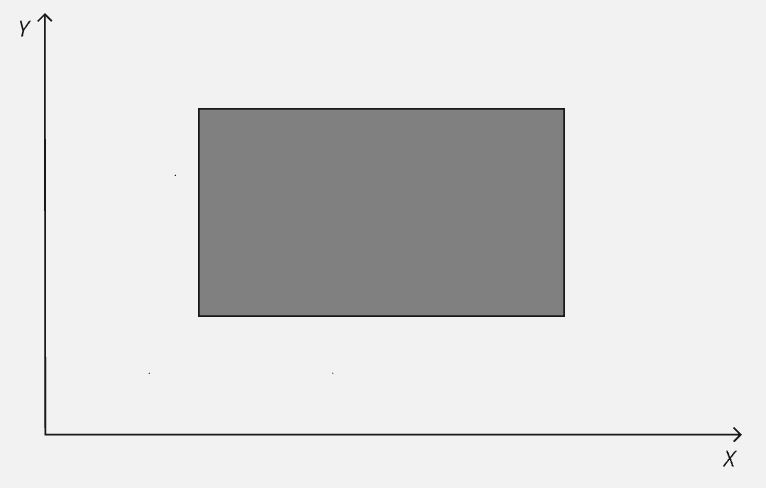
\includegraphics[width=\linewidth]{figures/Conceptos previos/Multi-intervalos/denso.png}
    \caption{Multi-intervalo denso — línea continua}
  \end{subfigure}
  \hfill
  \begin{subfigure}[b]{0.48\textwidth}
    \centering
    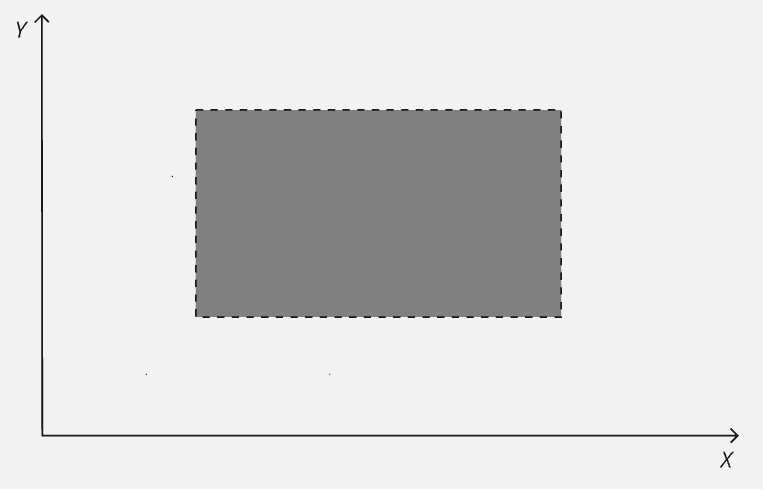
\includegraphics[width=\linewidth]{figures/Conceptos previos/Multi-intervalos/no-denso.png}
    \caption{Multi-intervalo no denso — línea discontinua}
  \end{subfigure}
  \caption{Representación de multi-intervalos bidimensionales}
  \label{fig:multiintervalos}
\end{figure}

Adicionalmente, se incluirá una representación gráfica que resalta el elemento mínimo y máximo de un multi-intervalo. Para ello, se utilizará un punto verde para indicar el mínimo y un punto rojo para el máximo. En la Figura~\ref{fig:multi} se muestra esta representación de manera ilustrativa.

\begin{figure}[ht]
  \centering
  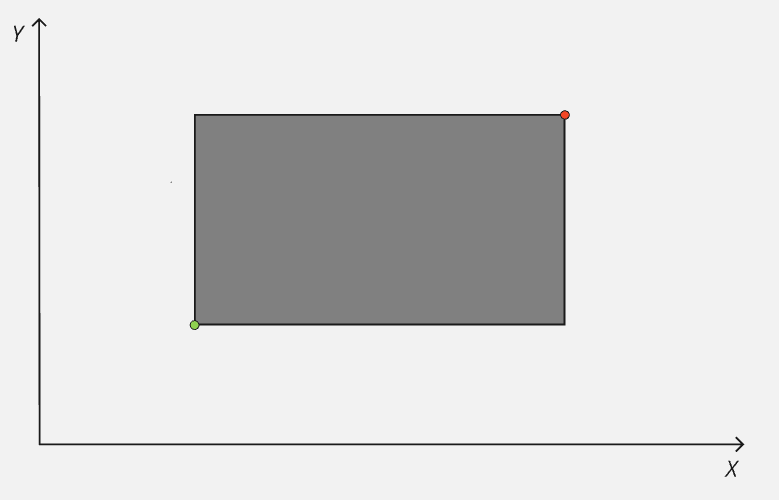
\includegraphics[width=0.6\textwidth]{figures/Conceptos previos/Multi-intervalos/minmax.png}
  \caption{Representación de un multi-intervalo con su mínimo (verde) y máximo (rojo).}
  \label{fig:multi}
\end{figure}


\section{Conjuntos}

\begin{center}
    \textit{Se modela un conjunto como una familia o colección de multi-intervalos no vacíos de igual cantidad de dimensiones y disjuntos dos a dos, es decir, no comparten ningún valor multi-dimensional d entre ellos.}
\end{center}

En consecuencia, la dimensión de un conjunto no está determinada por la cantidad total de multi-intervalos que lo componen, sino que corresponde a la dimensión de cualquiera de ellos.

La notación que se le dará a los conjuntos será la siguiente:

\begin{center}


    $\{i_{00} \times i_{01} \ \ldots \ \times i_{0(k-1)},\ i_{10} \times i_{11} \ \ldots \ \times i_{1(k-1)}\, \ldots,\ i_{(i-1)0} \times i_{(i-1)1} \ \ldots \ \times i_{(i-1)(k-1)}\}$
    
    Omitiendo los multi-intervalos:
    
    $\{mdi_0,\ mdi_1\ \ldots,\ mdi_{i-1}\}$

    donde $i$ es la cantidad de multi-intervalos del conjunto y $k$ es la cantidad de dimensiones que tendrán los mismos.
\end{center}

En particular, el conjunto vacío se representará de la siguiente manera: $\{\}$. Y en particular se utilizara la notación $\kappa(A)$ para representar la cantidad de multi-intervalos del conjunto $A$.


En primera instancia se verán todas las funciones relevantes que los conjuntos tienen disponibles en términos generales, ya que en el proyecto se disponen de múltiples implementaciones de conjuntos.

\subsection{Conjuntos generales}


La estructura \texttt{SetDelegate} representa un tipo base abstracto que define una interfaz común para manipulación de conjuntos de multi-intervalos. Este tipo se define como parte del conocido patrón de diseño \textit{delegate}, utilizado en este contexto para encapsular distintas implementaciones concretas de conjuntos dentro de una estructura delegadora. Esta estructura delegadora corresponde al tipo \texttt{Set}. De este modo, siempre que se requiera trabajar con conjuntos fuera de su implementación, se empleará una instancia de \texttt{Set}, la cual contendrá una implementación concreta de conjuntos del tipo \texttt{SetDelegate}.


Entre estas implementaciones concretas se encuentran: \texttt{UnorderedSet}, que representa conjuntos desordenados; y \texttt{OrderedDenseSet}, que modela conjuntos ordenados densos, es decir, con una única dimensión y con paso igual a uno. A partir de aquí.


Se han definido las siguientes operaciones sobre los conjuntos en la interfaz propuesta por \texttt{SetDelegate} :

\begin{itemize}
    \begin{comment}
    
    %sacable
    \item \texttt{SetDelegate() (Sin argumentos):}  
    Crea un conjunto vacío, es decir, $\{\}$.
    %sacable
    \item \texttt{SetDelegate(const MD\_NAT \&x):}  
    Crea un conjunto con un único multi-intervalo utilizando a $x$.
%sacable
    \item \texttt{SetDelegate(const Interval \&i):}  
    Crea un conjunto con un único multi-intervalo que solo contiene a $i$.
%sacable
    \item \texttt{SetDelegate(const SetPiece \&mdi):}  
     Crea un conjunto con un único multi-intervalo $mdi$.
    \end{comment}

    \item \texttt{virtual bool operator==(const SetDelegate \&other) const = 0:}  
    Verifica que los dos conjuntos tengan exactamente los mismos elementos.

    \begin{center}
        \textbf{Por ejemplo:} $\{[0: 1: 10] \times [11: 1: 20] \times [21: 1: 21]\}\texttt{==}\{[0: 1: 10] \times [11: 1: 20] \times [21: 1: 21]\}=\texttt{true}$.
    \end{center}

    \item \texttt{virtual bool operator!=(const SetDelegate \&other) const = 0:}  
    Verifica que los dos conjuntos no ten

    \begin{center}
        \textbf{Por ejemplo:} $\{[0: 1: 10] \times [11: 1: 20] \times [21: 1: 21]\}\texttt{!=}\{\}=\texttt{true}$.
    \end{center}

    \item \texttt{virtual std::size\_t size() const = 0:}
     Devuelve la cantidad de multi-intervalos en el conjunto.

    \begin{center}
        \textbf{Por ejemplo:} $size(\{[0: 1: 10] \times [11: 1: 20] \times [21: 1: 21]\})=1$.
    \end{center}
     
     \item \texttt{virtual void emplaceBack(const SetPiece \&mdi) = 0:}
     Agrega un multi-intervalo $mdi$ más al final del conjunto.

    \begin{center}
        \textbf{Por ejemplo:} $emplaceBack(\{[0: 1: 10] \times [11: 1: 20] \times [21: 1: 21]\}, [11: 1: 21] \times [11: 1: 20] \times [21: 1: 21])=\{[0: 1: 10] \times [11: 1: 20] \times [21: 1: 21], [11: 1: 21] \times [11: 1: 20] \times [21: 1: 21]\}$.
    \end{center}

     \item \texttt{virtual void emplace(const SetPiece \&mdi) = 0:}
     Agrega un multi-intervalo $mdi$ en algún lugar, donde corresponda, del conjunto.

     \begin{center}
        \textbf{Por ejemplo:} $emplace(\{[0: 1: 10] \times [11: 1: 20] \times [21: 1: 21]\},$
        
        $ [11: 1: 21] \times [11: 1: 20] \times [21: 1: 21])=$
        
        $\{[0: 1: 10] \times [11: 1: 20] \times [21: 1: 21], [11: 1: 21] \times [11: 1: 20] \times [21: 1: 21]\}$.
    \end{center}
    
    \item \texttt{virtual unsigned int cardinal() const = 0:}  
    Devuelve la cantidad de elementos contenidos en el conjunto. En escancia la suma del cardinal de todos los multi-intervalos que lo conforman.

     \begin{center}
        \textbf{Por ejemplo:} $cardinal(\{[0: 1: 10]\})=11$.
    \end{center}

    \item \texttt{virtual bool isEmpty() const = 0:}  
    Verifica si un conjunto es vacío, es decir, no contiene multi-intervalos.

         \begin{center}
        \textbf{Por ejemplo:} $isEmpty(\{[0: 1: 10]\})=\texttt{false}$.
    \end{center}

    \item \texttt{virtual MD\_NAT minElem() const = 0:}  
    Devuelve el mínimo elemento del conjunto.

    \begin{center}
        \textbf{Por ejemplo:} $minElem(\{[0: 1: 10], [15: 1: 100]\})=0$.
    \end{center}

    \item \texttt{virtual MD\_NAT maxElem() const = 0:}  
    Devuelve el máximo elemento del conjunto.

    \begin{center}
        \textbf{Por ejemplo:} $maxElem(\{[0: 1: 10], [15: 1: 100]\})= 100$.
    \end{center}

    \item \texttt{virtual SetDelegPtr intersection(const SetDelegate \&other) const = 0):}  
    Realiza la intersección entre el conjunto que invoca el método y el conjunto $other$. Si estos no tienen elementos en común, devuelve el conjunto vació.

    \begin{center}
        \textbf{Por ejemplo:} $intersection(\{[0: 1: 100], [500: 1: 1000]\},\{[1000: 1: 10000]\})= \{[1000: 1: 1000]\}$.
    \end{center}

    \item \texttt{virtual SetDelegPtr cup(const SetDelegate \&other) const = 0:}  
    Realiza la union entre el conjunto que invoca el método y el conjunto $other$.

    \begin{center}
        \textbf{Por ejemplo:} $cup(\{[0: 1: 100], [500: 1: 1000]\},\{[500: 1: 1000],[1400: 1: 10000]\})=$
        
        $ \{[0: 1: 100],[500: 1: 1000],[1400: 1: 10000]\}$.
    \end{center}

    \item \texttt{virtual SetDelegPtr complement() const = 0:}  
    Obtiene el complemento del conjunto que invoca el método.

    
    \begin{center}
        \textbf{Por ejemplo:} $complement(\{[10: 1: 100]\})= \{[0: 1: 9],[101: 1: \texttt{Inf}]\}$.
    \end{center}

    \item \texttt{virtual SetDelegPtr difference(const SetDelegate \&other) const = 0:}  
    Realiza la diferencia entre el conjunto que invoca el método y el conjunto $other$, es decir, al invocante se le resta $other$.

    \begin{center}
        \textbf{Por ejemplo:} $difference(\{[1: 1: 2], [3: 1: 100]\},\{[50: 1: 100]\})= \{[1: 1: 2], [3: 1: 49]\}$.
    \end{center}
    
        
    \item \texttt{virtual std::size\_t arity() const = 0}:  
    Devuelve la cantidad de dimensiones que tiene el conjunto, es decir, la aridad de los multi-intervalos que lo componen.

    \begin{center}
        \textbf{Por ejemplo:} $arity(\{[0: 1: 10] \times [11: 1: 20] \times [21: 1: 21]\})=3$.
    \end{center}
    
    \item \texttt{virtual SetDelegPtr disjointCup(const SetDelegate \&other) const = 0:}  
    Realiza la unión disjunta entre el conjunto que invoca el método y el conjunto $other$. Se asume que los argumentos son conjuntos disjuntos.

    \begin{center}
        \textbf{Por ejemplo:} $disjointCup(\{[1: 1: 2], [3: 1: 100]\},\{[0: 1: 0],[1000: 1: 3000]\})=\{[1: 1: 2],$
        
        $ [3: 1: 100],[0: 1: 0],[1000: 1: 3000]\}$.
    \end{center}
    
    \begin{comment}
%sacable
    \item \texttt{virtual SetDelegPtr filterSet(bool (*f)(const SetPiece \&mdi)) const = 0:}  
    Devuelve un conjunto con aquellos multi-intervalos que hayan pasado el predicado $f$.
%sacable
    \item \texttt{virtual SetDelegPtr offset(const MD\_NAT \&off) const = 0:}  
    Devuelve un conjunto con todos los elementos del conjunto que invoco al método desplazados un offset $off$, es decir, se le aplica el método offset con $off$ a cada multi-intervalo.
    \end{comment}
    \item \texttt{virtual SetDelegPtr compact() const = 0:}  
    Devuelve el conjunto resultante de intentar compactar los distintos multi-intervalos del conjunto que invoca el método con el resto de los multi-intervalos.

    \begin{center}
        \textbf{Por ejemplo:} $compact(\{[0: 1: 10] \times [11: 1: 20] \times [21: 1: 21]\})= \{[0: 1: 21]\}$.
    \end{center}

\end{itemize}


Para cumplir con el objetivo de proporcionar una implementación concreta de conjuntos ordenados, se decidió tomar como punto de partida la implementación ya existente de conjuntos desordenados. 

Aunque, como se indicó anteriormente, no es el propósito de este documento detallar dichas implementaciones previas, se explicará con mayor profundidad el funcionamiento de la operación \texttt{complement} en el caso de conjuntos desordenados, ya que se considera útil especialmente para facilitar y modularizar la comprensión de las optimizaciones propuestas.


Asimismo, se incluirá una descripción más breve de otras operaciones relevantes, tales como \texttt{intersection} y \texttt{disjointCup}.

\subsection{Conjuntos desordenados}\label{sec:conjs-des}

Cabe destacar que la estructura \texttt{UnorderedSet} se encuentra compuesta exclusivamente por una colección de multi-intervalos, almacenada en una variable denominada \texttt{pieces\_}. Esta colección se implementa mediante un contenedor de tipo \texttt{vector<SetPiece>}.

\textbf{Pseudocódigo/Notación:} En este capítulo los diferentes multi-intervalos de un conjunto desordenado se indexarán mediante subíndices. En particular, $A_i$ representará el $i$-ésimo multi-intervalo del conjunto desordenado $A$, lo cual corresponde a \texttt{pieces\_[i]} en C++, con $i \in \{0, \ldots, \kappa(A)-1\}$.

\subsubsection{Intersección - \texttt{intersection}}

Como se puede observar en el Algoritmo~\ref{alg:interseccionDes} el pseudocódigo para la operación \texttt{intersection}, la implementación de la intersección entre conjuntos desordenados resulta, en esencia, relativamente simple y directa, si se excluyen los casos especiales que optimizan su ejecución. 

El enfoque central de esta operación consiste en iterar sobre todos los multi-intervalos que conforman el conjunto desordenado $A$ y, para cada uno de ellos, computar su intersección con todos los multi-intervalos del conjunto desordenado $B$. De esta forma, se construye un nuevo conjunto cuyos elementos corresponden a las intersecciones no vacías entre los pares de multi-intervalos provenientes de $A$ y $B$ respectivamente.

\begin{algorithm}
\caption{Intersección entre conjuntos desordenados}\label{alg:interseccionDes}
\begin{algorithmic}[1]
\Require $A$, $B$ son conjuntos desordenados
\Ensure $C$ es un conjunto desordenado que representa $A \cap B$
\Function{intersection}{$A, B$}

\State $C := \{\}$

\If{$\Call{isEmpty}{A}$ \textbf{or} $\Call{isEmpty}{B}$}
    \State \Return $C$
\EndIf

\If{$\Call{maxElem}{A} < \Call{minElem}{B}$ \textbf{or} $\Call{maxElem}{B} < \Call{minElem}{A}$}
    \State \Return $C$
\EndIf

\If{$\Call{maxElem}{A} == \Call{minElem}{B}$}
    \State $C := \{ \Call{maxElem}{A} \}$
    \State \Return $C$
\EndIf

\If{$\Call{maxElem}{B} == \Call{minElem}{A}$}
    \State $C := \{\Call{minElem}{A} \}$
    \State \Return $C$
\EndIf

\If{$A == B$}
    \State \Return $A$
\EndIf

\

\ForAll{$a \in A$}
    \ForAll{$b \in B$}
        \State $mdi := \Call{intersection}{a,b}$
        \If{$i \neq \emptyset$}
            \State $\Call{emplaceBack}{C,mdi}$
        \EndIf
    \EndFor
\EndFor

\State \Return $C$
\EndFunction
\end{algorithmic}
\end{algorithm}

\subsubsection{Complemento - \texttt{complement}}

El cálculo del complemento de conjuntos desordenados se define a partir de dos funciones principales: \texttt{complement} y \texttt{complementAtom}. 

La función \texttt{complement} es la encargada de realizar el cálculo general del complemento para un conjunto arbitrario con ayuda de la operación \texttt{intersection}, mientras que \texttt{complementAtom} se especializa en calcular el complemento de un conjunto que contiene únicamente un multi-intervalo.

A continuación, se detalla el funcionamiento específico de ambas funciones.


\textbf{Complement}

La operación de complemento, denominada \texttt{complement}, permite calcular el complemento de un conjunto desordenado compuesto por una cantidad variable de multi-intervalos. En el pseudocódigo, Algoritmo~\ref{alg:complementDes}, se presenta la operación \texttt{complement}, donde se ilustra su funcionamiento.  

Desde una perspectiva teórica de conjuntos, la operación busca calcular la siguiente expresión:

\[
\bigcap_{i=0}^{ \kappa(A)-1} \overline{\{A_i\}}
\]

La cual se fundamenta en que:

\[
A = \{A_0, A_1, A_2, \ldots, A_{\kappa(A)-1}\} 
    = \bigcup_{i=0}^{\kappa(A)-1} \{A_i\}
\]

y, por lo tanto,

\[
\overline{A} 
    = \overline{\bigcup_{i=0}^{\kappa(A)-1} \{A_i\}}
    = \bigcap_{i=0}^{\kappa(A)-1} \overline{\{A_i\}}.
\]



\begin{comment}
Aquí se describe la operación principal que permite calcular el complemento de un conjunto desordenado con una cantidad variable de multi-intervalos, \texttt{complement}. Seguidamente, se presenta el pseudocódigo de la operación ~\ref{alg:complementDes}, junto con el procedimiento que se lleva a cabo:



\begin{enumerate}
    \item En primer lugar, se calcula el complemento de un conjunto atómico compuesto únicamente por el primer multi-intervalo del conjunto $A$, utilizando la función \textit{complementAtom} y guardándolo como resultado final en $C$. Esta función será explicada más adelante; por ahora, basta con saber que genera un conjunto desordenado que representa el complemento de un conjunto formado por un único multi-intervalo.
    
    \item Luego, se calcula el \textit{complementAtom} del siguiente multi-intervalo del conjunto $A$, en caso de que exista, y se realiza la intersección entre el resultado actual $C$ y el conjunto complemento resultante de dicho multi-intervalo.
    
    \item Finalmente, se guarda el resultado de la intersección y se repite desde el paso anterior hasta que no queden más multi-intervalos por recorrer en $A$. Posteriormente se devuelve $C$, que es el complemento de $A$.
\end{enumerate}

\end{comment}



\begin{algorithm}
\caption{Complemento de un conjunto desordenado}\label{alg:complementDes}
\begin{algorithmic}[1]
\Require $A$ es un conjunto desordenado 
\Ensure $C$ es un conjunto desordenado que representa el complemento de $A$
\Function{complement}{$A$}
\State $C := \{\}$
\State $first\_mdi := A_0$
\State $C :=$  \Call{complementAtom}{$first\_mdi$} 
\For{$i := 1$; $i\neq size(A)$; $i$\!+\!+}
    \State $mdi := A_i$
    \State $atomic\_set :=$ \Call{complementAtom}{$mdi$}
    \State $C :=$ \Call{intersection}{$C$,$atomic\_set$}
\EndFor
\State \textbf{return} $C$
\EndFunction
\end{algorithmic}
\end{algorithm}



En la Figura~\ref{fig:complemento} se muestra gráficamente cómo se va calculando el complemento de un conjunto desordenado. En particular en este ejemplo el conjunto $A$ tiene solo multi-intervalos densos. Se eligieron multi-intervalos densos para que la representación gráfica sea mas sencilla de comprender.

\begin{figure}[H]
    \centering
    
    % Imagen principal grande
    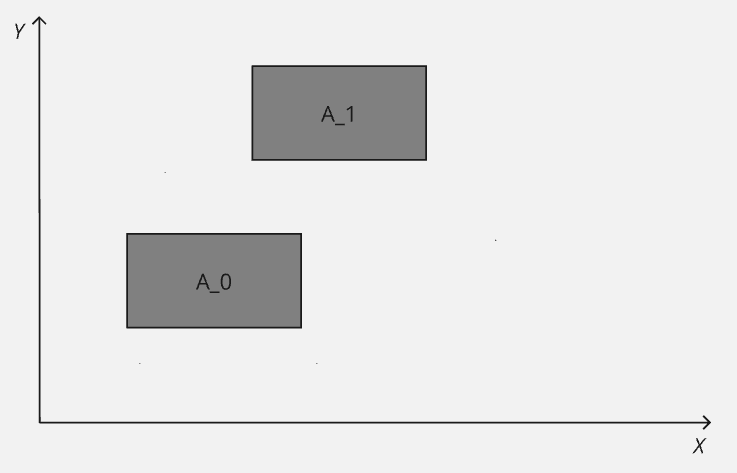
\includegraphics[width=0.6\textwidth]{figures/Conceptos previos/Conjuntos/conjuntoAcomp.png}
    \caption*{(a) Conjunto desordenado $A$}
    
    \vspace{1em}
    
    % Subfiguras en 3 columnas (6 imágenes en total)
    \begin{minipage}{0.31\textwidth}
        \centering
        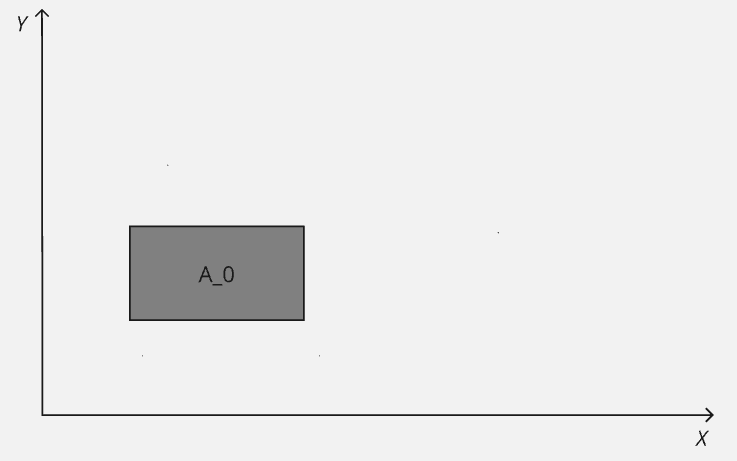
\includegraphics[width=\textwidth]{figures/Conceptos previos/Conjuntos/iter1comp.png}
        \caption*{    \centering (b1) Conjunto atómico con $A_0$}
    \end{minipage}
    \begin{minipage}{0.31\textwidth}
        \centering
        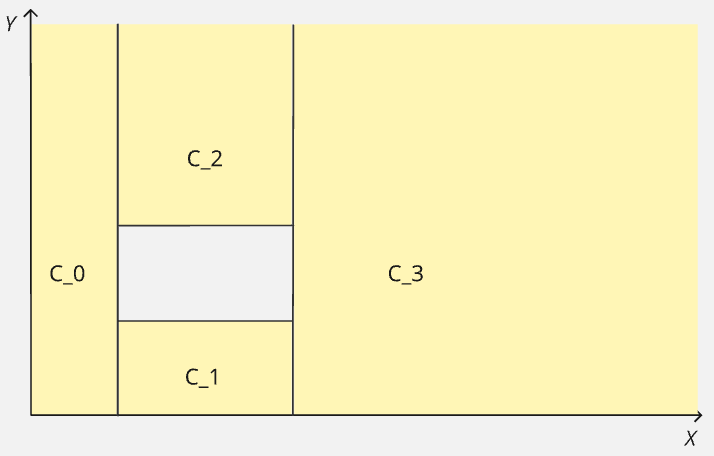
\includegraphics[width=\textwidth]{figures/Conceptos previos/Conjuntos/iter1compA.png}
        
        \caption*{     \centering (b2) Complemento del conjunto atómico}
    \end{minipage}
    \begin{minipage}{0.31\textwidth}
        \centering
        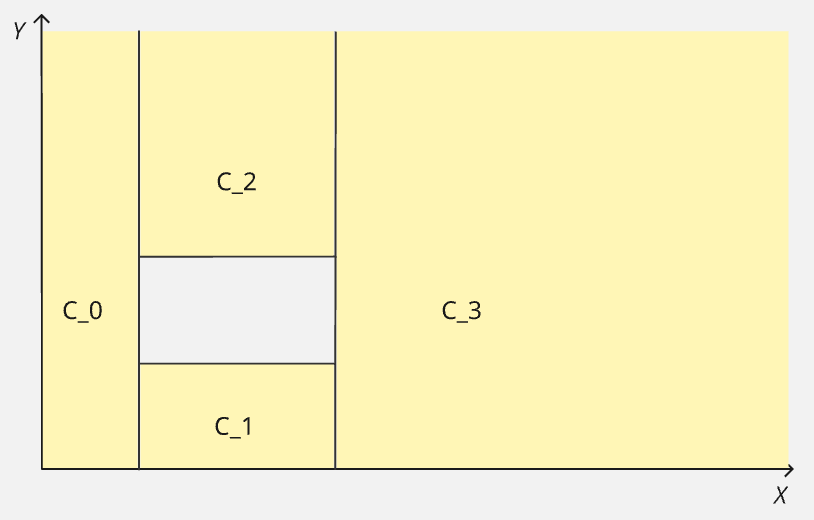
\includegraphics[width=\textwidth]{figures/Conceptos previos/Conjuntos/C1comp.png}
        \caption*{    \centering (b3) Conjunto $C$}
    \end{minipage}
    
    \vspace{1em}
    
    \begin{minipage}{0.31\textwidth}
        \centering
        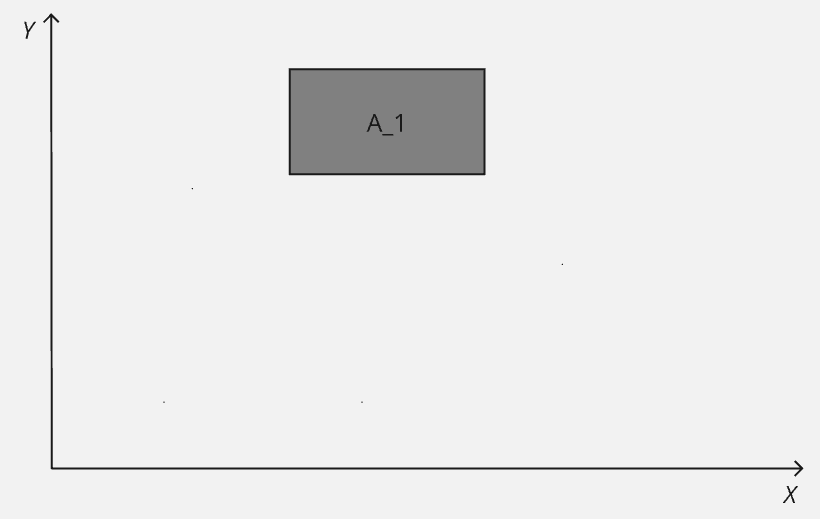
\includegraphics[width=\textwidth]{figures/Conceptos previos/Conjuntos/iter2comp.png}
        \caption*{    \centering (b4) Conjunto atómico con $A_1$}
    \end{minipage}
    \begin{minipage}{0.31\textwidth}
        \centering
        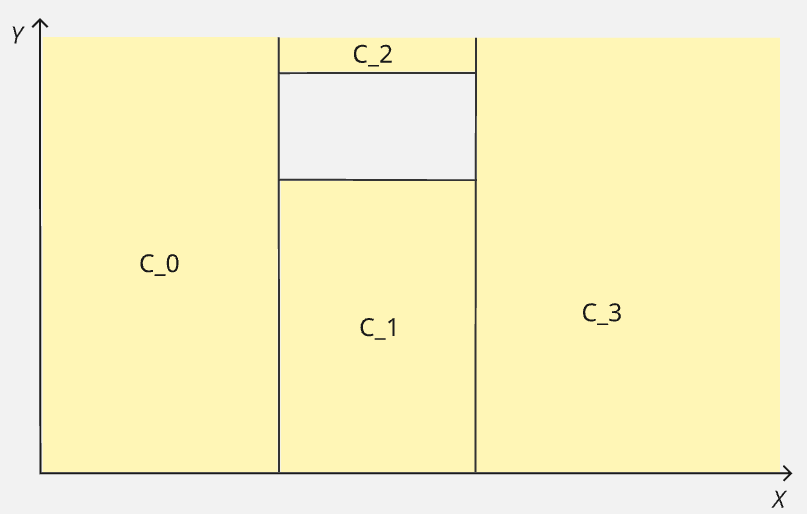
\includegraphics[width=\textwidth]{figures/Conceptos previos/Conjuntos/iter2compA.png}
        \caption*{    \centering (b5) Complemento del conjunto atómico}
    \end{minipage}
    \begin{minipage}{0.31\textwidth}
        \centering
        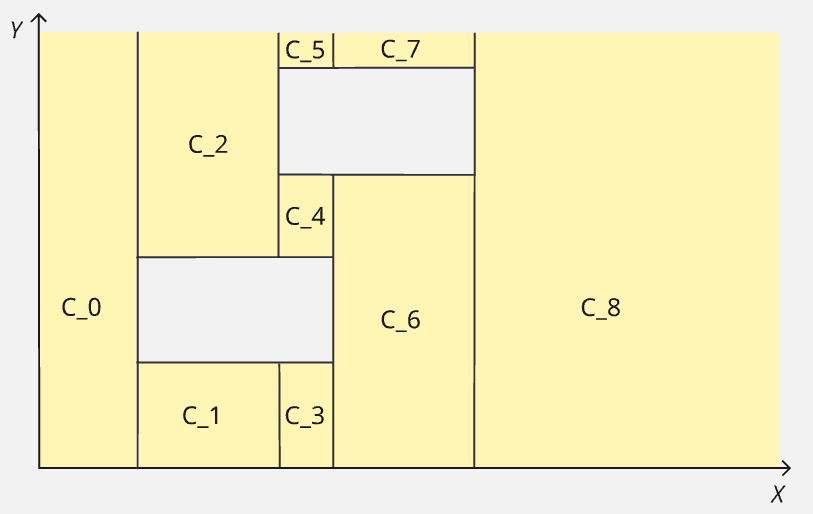
\includegraphics[width=\textwidth]{figures/Conceptos previos/Conjuntos/C2comp.png}
        \caption*{    \centering (b6) Conjunto $C$}
    \end{minipage}
    
    \caption{Visualización del cálculo del complemento de un conjunto desordenado con multi-intervalos densos $A$.}
    \label{fig:complemento}
\end{figure}


\textbf{ComplementAtom}

Una vez descrita la operación \texttt{complement} de conjuntos desordenados, lo único que resta por detallar es cómo se calcula el complemento de un conjunto desordenado que contiene un único multi-intervalo. Esta tarea es realizada por la operación \textit{complementAtom}.  
El procedimiento que dicha operación lleva a cabo se encuentra plasmado en el pseudocódigo de la operación en el Algoritmo~\ref{alg:ComplementAtomDes}, y puede explicarse de la siguiente manera:

\begin{enumerate}
    \item Se inicia el proceso con tres multi-intervalos fundamentales: $dense\_mdi$, que tiene la misma disposición de intervalos que el del conjunto original, pero con paso 1 en todos ellos(representando al multi-intervalo en su versión completamente densa); $during\_mdi$, que inicialmente es una copia de $dense\_mdi$ y $all$, que representa el multi-intervalo universo, con la misma aridad que el multi-intervalo del conjunto.

  \item Ahora bien, para calcular el complemento del conjunto atómico, se tendrán que recorrer una a una las dimensiones del multi-intervalo interno con la siguiente lógica:
  \begin{enumerate}
    \item \textbf{Selección de la dimensión.}  
      Se empieza por la dimensión \(d=0\). Y se extrae en base a ella el intervalo original del multi-intervalo del cual se quiere obtener el complemento: 
      \[
        d = [d_{\mathrm{begin}}:d_{\mathrm{step}}:d_{\mathrm{end}}].
      \]
    \item \textbf{Región “antes” del intervalo.}  
      Si \(d_{\mathrm{begin}}>0\), existe un rango no cubierto entre \(0\) y \(d_{\mathrm{begin}}-1\). Entonces se toma el multi-intervalo universo \(\mathit{all}\) y se lo restringe en la dimensión \(d\) a  
      \[
        [0:1:d_{\mathrm{begin}}-1].
      \]
      dejando los intervalos de las demás dimensiones sin cambios. Esa variación de \(\mathit{all}\) se añade al conjunto parcial de resultados $C$ y luego deshace el cambio.
    \item \textbf{Huecos “durante” el intervalo.}  
      Si el paso \(d_{\mathrm{step}}>1\), el intervalo original salta posiciones; entre cada salto quedan “huecos” que también forman parte del complemento. Para cada \(j=0,\dots,d_{\mathrm{step}}-2\) construimos  
      \[
        [d_{\mathrm{begin}}+j+1:d_{\mathrm{step}}:d_{\mathrm{end}}],
      \]
      y lo insertamos en una copia de nuestro multi-intervalo base, $during\_mdi$, y lo metemos en el conjunto desordenado resultante $C$.
      
    \item \textbf{Región “después” del intervalo.}  
      Si \(d_{\mathrm{end}}<\ \texttt{Inf}\), hay un rango desde \(d_{\mathrm{end}}+1\) hasta \texttt{Inf} de valores no abarcados por $i$. De nuevo se usa \(\mathit{all}\) restringido en \(d\) a  
      \[
        [i_{\mathrm{end}}+1:1: \texttt{Inf}],
      \]
       se lo añade al conjunto de resultados y se revierte el cambio de $all$.
    \item \textbf{Restauración y avance.}  
      Tras procesar el “antes”, “durante” y “después” en la dimensión \(d\), se actualizan \(\mathit{all}\) y $during\_mdi$, colocándoles los valores densos y originales de la dimensión \(d\) del multi-intervalo del cual estamos sacando el complemento respectivamente. Luego se pasa a la siguiente dimensión \(d+1\), y se repite todo el procedimiento.
  \end{enumerate}
\end{enumerate}

En la Figura a siguiente se muestra gráficamente cómo se va calculando el complemento atómico de un conjunto desordenado con un único multi-intervalo. En particular en este ejemplo el conjunto tiene un solo multi-intervalo no denso.
 
\begin{figure}[H]
    \centering
    
    % Imagen principal grande
    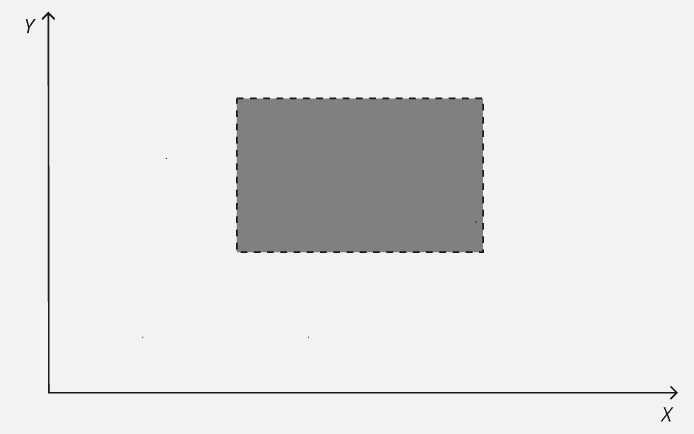
\includegraphics[width=0.6\textwidth]{figures/Conceptos previos/Conjuntos/compAtom1.png}
    \caption*{(a) Conjunto desordenado atómico}
    
    \vspace{1em}
    \begin{minipage}{0.41\textwidth}
        \centering
        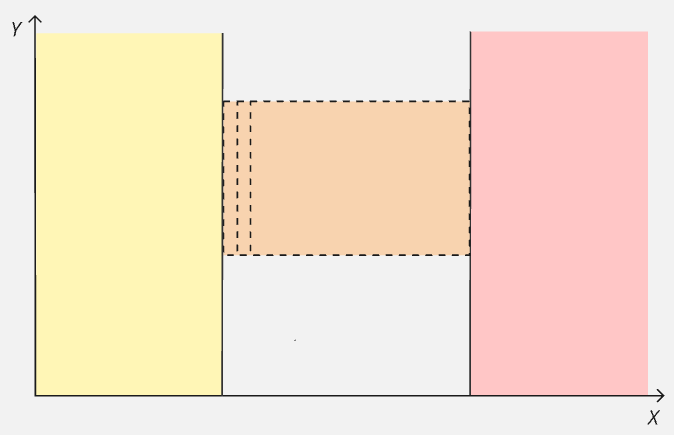
\includegraphics[width=\textwidth]{figures/Conceptos previos/Conjuntos/compAtom2.png}
        
        \caption*{     \centering (b1) Multi-intervalos resultantes del complemento atómico sobre la primera dimensión $x$}
    \end{minipage}
    \begin{minipage}{0.41\textwidth}
        \centering
        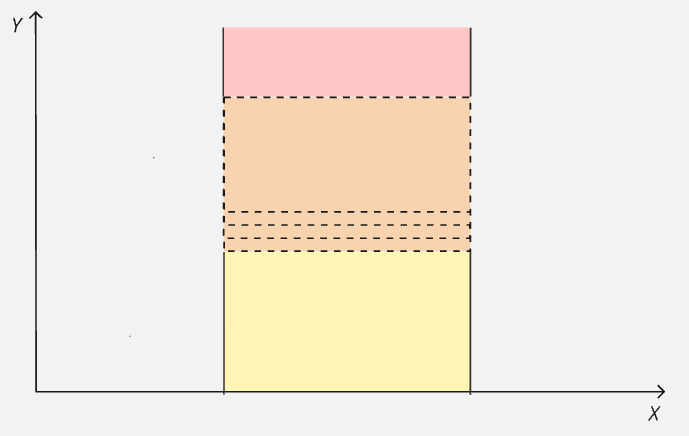
\includegraphics[width=\textwidth]{figures/Conceptos previos/Conjuntos/compAtom3.png}
        \caption*{    \centering (b2) Multi-intervalos resultantes del complemento atómico sobre la segunda dimensión $y$}
    \end{minipage}
    
    \caption{Visualización del cálculo del complemento atómico sobre un conjunto desordenado atómico no denso.}
    \label{fig:complemento}
\end{figure}

\begin{algorithm}
\caption{Complemento atómico de conjunto ordenado atómico}
\label{alg:ComplementAtomDes}
\begin{algorithmic}[1]
\Require $A$ es un conjunto ordenado atómico
\Ensure Un conjunto desordenado $C$, el complemento de $A$
\Function{complementAtom}{$A$}
  \State $C := \emptyset$  
  \State $mdi := A_0$  
  \State $dense\_mdi := ||$
  \ForAll{$interval \in mdi$}
    \State $i := $$[$\Call{begin}{$interval$} $:1:$ \Call{end}{$interval$}$]$
    \State \Call{emplaceBack}{$dense\_mdi,i$}
  \EndFor

  \State $during\_mdi := dense\_mdi$
  \State $univ := [0:1:\texttt{Inf}]$
  \State $all := |univ|^{\Call{arity}{A}}$ \Comment{Representa el universo completo de aridad $\Call{arity}{A}$}

  \State $dim := 0$
  \ForAll{$i \in mdi$}

    \If{\Call{begin}{$i$} $\neq 0$}
      \State $i\_res := [0:1:$ \Call{begin}{$i$}$-1]$
      \If{$\neg \Call{isEmpty}{i\_res}$}
        \State $all[dim] := i\_res$
        \State $C := C \frown \{all\}$
        \State $all[dim] := univ$
      \EndIf
    \EndIf

    \If{\Call{begin}{$i$} $<$ \texttt{Inf}}
        \If{\Call{step}{$i$} $> 1$}
          \For{$j = 0$; $i < size(A)$; $j$\!+\!+}
            \State $h := [$\Call{begin}{$i$}$ + j + 1 : $\Call{step}{$i$} $: $ \Call{end}{$i$}$]$
            \If{$\neg \Call{isEmpty}{h}$}
              \State $during\_mdi[dim] := h$
              \State $C := C \frown during\_mdi$
            \EndIf
          \EndFor
        \EndIf
    \EndIf

    \If{\Call{end}{$i$} $<$ \texttt{Inf}}
      \State $i\_res := [$\Call{end}{$i$}$+1 : 1 : \texttt{Inf}]$
      \If{$\neg \Call{isEmpty}{i\_res}$}
        \State $all[dim] := i\_res$
        \State $C := C \frown \{all\}$
        \State $all[dim] := univ$
      \EndIf
    \EndIf

    \State $all[dim] := dense\_mdi[dim]$
    \State $during\_mdi[dim] := i$
    \State $dim \!+\!+$
  \EndFor
  \State \Return $C$
\EndFunction
\end{algorithmic}
\end{algorithm}


\begin{comment}
\subsubsection{Diferencia - \texttt{defference}}

Al igual que ocurre con la operación de unión (la cual será abordada más adelante), la disponibilidad previa de las operaciones de intersección y complemento permite implementar la diferencia de conjuntos desordenados de manera sencilla. Esta estrategia modular se refleja claramente en la simplicidad de la función \texttt{difference}, cuyo pseudocódigo se presenta en ~\ref{alg:differenceDes} y que constituye precisamente la operación encargada de calcular la diferencia entre conjuntos desordenados.


\begin{algorithm}
\caption{Diferencia de conjuntos desordenados}\label{alg:differenceDes}
\begin{algorithmic}[1]
\Require $A$, $B$ son conjuntos desordenados
\Ensure $C$ es el conjunto $A \setminus B$
\Function{difference}{$A$, $B$}

\If{$A == \emptyset$ \textbf{or} $B == \emptyset$}
    \State \textbf{return} $A$
\EndIf

\State $B' :=$ \Call{complement}{$B$}
\State $C:=$ \Call{intersection}{$A$, $B'$}

\State \textbf{return} $C$
\EndFunction
\end{algorithmic}
\end{algorithm}

    
\end{comment}


\subsubsection{Unión disjunta - \texttt{disjointCup}}

En lo que respecta a la operación correspondiente a la \textit{unión disjunta}(\texttt{disjointCup}), al igual que la intersección, se trata de una operación conceptualmente sencilla. Esta simplicidad se ve reflejada en el pseudocódigo del Algoritmo~\ref{alg:disjointcupDes}. Dado que los conjuntos involucrados son desordenados y, por hipótesis, disjuntos entre sí, la operación no requiere verificaciones adicionales de solapamiento o duplicación de elementos. Basta simplemente con reunir todos los multi-intervalos de ambos conjuntos en una único conjunto desordenado para obtener el resultado deseado.


\begin{algorithm}
\caption{Unión disjunta de dos conjuntos desordenados}\label{alg:disjointcupDes}
\begin{algorithmic}[1]
\Require $A$, $B$ son conjuntos desordenados
\Ensure $R$ es un conjunto desordenado que representa la unión disjunta de $A$ y $B$
\Function{disjointCup}{$A, B$}

\If{$\Call{isEmpty}{A}$}
  \State \Return $B$
\EndIf

\If{$\Call{isEmpty}{B}$ \textbf{or} $A == B$}
  \State \Return $A$
\EndIf

\State $R :=$ $A$
\ForAll{$b \in B$}
  \State $\Call{emplaceBack}{R,b}$
\EndFor

\State \Return $R$
\EndFunction
\end{algorithmic}
\end{algorithm}

\begin{comment}
\subsubsection{Unión - \texttt{cup}}

Como se explicó anteriormente, la operación de unión puede construirse a partir de operaciones ya disponibles, como lo son la diferencia y la unión disjunta. Esta reutilización de funciones básicas permite que el código de la unión resulte especialmente sencillo, ya que basta con aplicar las operaciones de conjuntos que, en conjuntos, son equivalentes a una unión de conjuntos. De esta manera, la implementación de la operación \texttt{cup} es particularmente compacta y clara.

\begin{algorithm}
\caption{Unión de conjuntos desordenados (\texttt{cup})}\label{alg:cup}
\begin{algorithmic}[1]
\Require $A$, $B$: conjuntos desordenados
\Ensure $R$: conjunto desordenado que representa la unión $A \cup B$
\Function{cup}{$A, B$}

\If{$A == \emptyset$}
  \State \Return $B$
\EndIf

\If{$B == \emptyset$  \textbf{or} $A == B$}
  \State \Return $A$
\EndIf

\If{$\max(A) < \min(B)$}
  \State $R := A$
  \ForAll{$\text{mdi} \in B$}
    \State \Call{emplaceBack}{$B, mdi$}
  \EndFor
  \State \Return $R$
\EndIf

\If{$\max(B) < \min(A)$}
  \State $R := B$
  \ForAll{$\text{mdi} \in A$}
    \State \Call{emplaceBack}{$A, mdi$}
  \EndFor
  \State \Return $R$
\EndIf

\State $D :=$ \Call{difference}{$A, B$}
\State \Return \Call{disjointCup}{$B, D$}

\EndFunction
\end{algorithmic}
\end{algorithm}   
\end{comment}


\subsection{Conjuntos ordenados densos}\label{sec:conjs-ord-dense}

A continuación, se presenta una breve descripción de cómo los conjuntos ordenados densos organizan los multi-intervalos de manera interna. Esta explicación resulta relevante dado que, por razones de conveniencia, se ha adoptado el mismo criterio de orden para los multi-intervalos contenidos en un conjunto ordenado.

En particular, los conjuntos ordenados densos emplean una variable miembro llamada \texttt{pieces\_}, de tipo \texttt{MDIOrdSet}, que es un sinónimo de \texttt{vector<SetPiece>}. Esta estructura almacena los multi-intervalos, los cuales se ordenan utilizando la operación $<$ definida para los multi-intervalos (\texttt{SetPiece}).

Internamente, el operador $<$ entre multi-intervalos evalúa si el mínimo del primer multi-intervalo es menor que el del segundo. Dado que los mínimos son de naturales multi-dimensionales(\texttt{MD\_NAT}), esta comparación se realiza mediante el operador $<$ definido para \texttt{MD\_NAT}. En si, el operador $<$ definido para el tipo \texttt{MD\_NAT} compara componente por componente dos \texttt{MD\_NAT}, siguiendo el siguiente criterio que luego se aplica a los mínimos de los multi-intervalos: 

\begin{center}
Sea $x = (x_0, x_1, \dots, x_{n-1})$ y $y = (y_0, y_1, \dots, y_{n-1})$ dos elementos de tipo \texttt{MD\_NAT}. Se define que $x < y$ si y sólo si existe un índice $j \in \{0, \dots, {n-1}\}$ tal que se cumplen simultáneamente las siguientes condiciones:
\end{center}

\begin{itemize}
    \item $x_j < y_j$, es decir, en la componente $j$, $x$ es menor que $y$;
    \item Para todo $i$ tal que $0 \leq i < j$, se cumple que $x_i = y_i$.
\end{itemize}

Ahora bien al trabajar con multi-intervalos de solo una dimensión, este operador de menor queda relegado a solo ser el $<$ tradicional de los naturales. Por ende dados los siguientes multi-intervalos de una dimensión:

\begin{center}
    
    $mdi_1 = |[0:3:9]|$, con mínimo 0.
    
    $mdi_2 = |[4:1:10]|$, con mínimo 4.
    
    $mdi_3 = |[2:2:4]|$, con mínimo 2.
    
\end{center}

Se tiene que el conjunto ordenado denso queda tal que así:

\begin{center}
    $\{mdi_1,\ mdi_3,\ mdi_2\}$
\end{center}

ya que:

\begin{center}
    $0 < 2 < 4$
\end{center}

\subsection{\textit{Abstract factory} para conjuntos}

Adicionalmente, se incorpora el patrón de diseño \textit{abstract factory}, aplicado a la creación de instancias del tipo \texttt{SetDelegate}. Para ello, se define la clase abstracta \texttt{SetAF}, que actúa como una interfaz común para diferentes fábricas concretas, como \texttt{UnordAF}, para conjuntos desordenados y \texttt{OrdDenseAF}, para conjuntos ordenados densos, cada una responsable de construir conjuntos con una representación interna específica.

Esta abstracción cobra especial relevancia en la sección de mapas. Allí, la fábrica de mapas (\texttt{MapAF}) extiende a \texttt{SetAF}, y reutiliza internamente una fábrica concreta de conjuntos para construir tanto dominios como imágenes de los mapas.

\section{Mapas lineales}

\begin{center}
\textit{
Un mapa lineal puede entenderse como una asociación entre un conjunto de multi-intervalos y una colección de expresiones lineales. Formalmente, un mapa lineal de aridad \( j \in \mathbb{N}\) se define como:
\[
\mathit{map} = \{ \mathit{mdi}_0,\ \mathit{mdi}_2,\ \ldots,\ \mathit{mdi}_{k-1} \} \mapsto [e_0,\ e_2,\ \ldots,\ e_{j-1}]
\]
donde cada $mdi_l$ es un multi-intervalo de aridad \( j \), con $l$ entre 0 y $k$ y con $k \in \mathbb{N}$, y cada \( e_i \), con $i$ entre 0 y $j$, es una expresión lineal de la forma \( m*x + h \), con $m,h \in \mathbb{Q}$.}  

\textit{
El dominio del mapa está conformado multi-intervalos, $mdi$, y cada expresión \( e_i \) se evalúa sobre la \( i \)-ésima dimensión de dichos multi-intervalos. En otras palabras, el dominio de \( e_i \) está compuesto por la colección de todos los intervalos que aparecen en la dimensión \( i \) de cada $mdi$ presente en el dominio.
}
\end{center}

Este concepto de mapa lineal coincide con el de función multidimensional cabe recalcar. Para afianzar la idea, véanse ejemplos en una, dos y tres dimensiones:

\medskip

\textbf{Ejemplo 1. Unidimensional}
\[
\mathit{map} = \{[0,1,2],[5,1,7]\}\mapsto[x+1].
\]
Por ejemplo: \((1)\!\mapsto\![2]\) \((6)\!\mapsto\![7]\)

\medskip

\textbf{Ejemplo 2. Bidimensional}
\[
\mathit{map}=\{[0,1,1]\times[0,1,1],[3,1,4]\times[3,1,4]\}
\mapsto[x_0+2,\;2*x_1-1].
\]
Por ejemplo:
\((0,1)\!\mapsto\![2,1],\;(3,4)\!\mapsto\![5,7].\)

\medskip

\textbf{Ejemplo 3. Tridimensional}
\[\;
\mathit{map} = \{[0,1,1]\times[0,1,1]\times[0,1,1],
                 [2,1,3]\times[2,1,3]\times[2,1,3]\}
\mapsto[x_{0},\;x_{1}+1,\;2*x_{2}-1].
\]
Por ejemplo:
\[
(1,0,1)\;\mapsto\;[1,1,1],\quad
(3,2,3)\;\mapsto\;[3,3,5].
\]

La estructura \textbf{Map} se utilizara para representar a los mapas lineales y esta constituida por lo que sigue:

\begin{itemize}
  \item \texttt{dom} (de tipo \textbf{Set}): representa el dominio del mapa.
  \item \texttt{exp} (de tipo \textbf{Exp}): contiene la(s) expresión(es) lineal(es) asociada(s).
    \item \texttt{fact} (de tipo \textbf{SetAF}): contiene una fábrica concreta utilizada para construir cualquier tipo de conjunto relacionado con el mapa
\end{itemize}

Cabe destacar que el tipo \texttt{Exp} representará una colección de expresiones lineales, es un sinónimo para \texttt{vector<LExp>}, donde \texttt{LExp} es tipo de estructura que representa a una única expresión lineal.

A continuación se presentan las operaciones que tienen a disposición los mapas:

\begin{itemize}

   \begin{comment}
       
    \item \texttt{Map(const SetAF \&fact):}
    Crea un mapa vacío, $\{\{\}_{\langle fact\rangle} \mapsto []\}$, a través la fabrica concreta de conjuntos $fact$ como referencia para su dominio.
        
    \item \texttt{Map(const SetAF \&fact, MD\_NAT x, Exp exp):}
    Construye un mapa que contiene un único elemento $x$, una $n$-upla, en su dominio basado en la fabrica concreta de conjuntos $fact$, y cuyas expresiones lineales son $exp$.
    \begin{center}
        \textbf{Por Ejemplo:} con $x = (1,2)$ y $exp = [x_0 + 2,\; x_1 + 3]$, el mapa resultante es $\{\{|[1:1:1]\times[2:1:2]|\}_{\langle fact\rangle} \mapsto [x_0 + 2,\; x_1 + 3]$\}.
       
    \end{center}

    \item \texttt{Map(const SetAF \&fact, Interval i, LExp le):}
    Crea un mapa cuyo dominio es el conjunto, construido a través de $fact$, de elementos del intervalo $i$, y su expresión lineal es $le$.
    \begin{center}
        \textbf{Por Ejemplo:} con $i = [1:1:5]$ y $le = 2*x$, se crea el mapa $\{\{|[1:1:5]|\}_{\langle fact\rangle} \mapsto [2*x]\}$.
    \end{center}

    \item \texttt{Map(const SetAF \&fact, SetPiece mdi, Exp exp):}
    Construye un mapa definido sobre un conjunto construido a partir de la fabrica concreta de conjuntos $fact$, con unicamente el multi-intervalo $mdi$, y con expresión lineal $exp$.
    \begin{center}
        \textbf{Por Ejemplo:} con $mdi = |[1:1:3] \times [0:1:2]|$ y $exp = [x_0 + 2,\; x_1 +3]$, el mapa resultante es $\{|[1:1:3] \times [0:1:2]|\}_{\langle fact\rangle} \mapsto [x_0 + 2,\; x_1 + 3]\}$.
    \end{center}

    \item \texttt{Map(const SetAF \&fact, Set s, Exp exp):}
    Construye un mapa cuyo dominio es el conjunto $s$ y su ley de aplicación es $exp$.
   \end{comment} 

    \item \texttt{bool operator==(const Map \&other) const:} Verifica si dos mapas son iguales, es decir, si sus dominios y expresiones son idénticos, o si sus dominios e imágenes son iguales en caso de que sea un mapa con una único expresión.
    \begin{center}
        \textbf{Por Ejemplo:} $\{[1:1:3]\} \mapsto [x] \,\texttt{==}\, \{[1:1:3]\} \mapsto [x] =  \textit{true}$.
    \end{center}

    \item \texttt{bool operator!=(const Map \&other) const:} Verifica si dos mapas son distintos.
    \begin{center}
        \textbf{Por Ejemplo:} $\{[1:1:3]\} \mapsto [x] \,\texttt{==}\, \{[1:1:3]\} \mapsto [x+1] =  \textit{true}$.
    \end{center}

    \item \texttt{Map operator+(const Map \&other) const:} Suma dos mapas realizando la intersección de sus dominios y sumando sus expresiones.
    \begin{center}
        \textbf{Por Ejemplo:} $\{[1:1:3]\} \mapsto  [x] + \{|[2:1:4]|\} \mapsto [2*x] = \{[2:1:3]\} \mapsto [3*x]$.
    \end{center}


    \item \texttt{std::size\_t arity() const:} Devuelve la aridad del dominio del mapa.
    \begin{center}
        \textbf{Por Ejemplo:} $arity(\{[1:1:5] \times [0:1:2]\} \mapsto [x,x]) = 2$.
    \end{center}

    \item \texttt{bool isEmpty() const:} Devuelve \texttt{true} si el mapa no tiene elementos en su dominio.
    \begin{center}
        \textbf{Por Ejemplo:} $isEmpty(\{\} \mapsto [x]) = \texttt{true}$.
    \end{center}

    \item \texttt{Map restrict(const Set \&subdom) const:} Restringe el dominio del mapa en base $subdom$.
    \begin{center}
        \textbf{Por Ejemplo:} $restrict(\{[0:1:10]\} \mapsto [x],\{[5:1:8]\}) = \{[5:1:8]\} \mapsto [x]$.
    \end{center}

    \item \texttt{Set image() const:} Devuelve el conjunto imagen del mapa.
    \begin{center}
        \textbf{Por Ejemplo:} $image(\{[0:1:3]\} \mapsto [2*x]) = \{[0:2:6]\}$.
    \end{center}

    \item \texttt{Set image(const Set \&subdom) const:} Imagen del mapa restringido por $subdom$.
    \begin{center}
        \textbf{Por Ejemplo:} $image(\{[0:1:3]\} \mapsto [2*x],\{[1:1:1]\}) = \{[2:1:2]\}$.
    \end{center}

    \item \texttt{Set preImage(const Set \&subcodom) const:} Preimagen del subconjunto de la imagen $subcodom$.
    \begin{center}
        \textbf{Por Ejemplo:} $preImage(\{[0:1:3]\} \mapsto [2*x],\{[4:1:4]\}) = \{[2:1:2]\}$.
    \end{center}

    \item \texttt{Map composition(const Map \&other) const:} Composición de mapas.
    \begin{center}
        \textbf{Por Ejemplo:} $composition(\{[0:1:3]\} \mapsto [x+1],\{[0:1:3]\} \mapsto [2*x]) = \{[0:1:3]\} \mapsto [2*x+1]$.
    \end{center}

    \item \texttt{Map minInv() const:} Calcula la inversa o pseudo-inversa de un mapa.
    \begin{center}
                \textbf{Por Ejemplo:}$composition(\{[5:1:10]\} \mapsto [x+1]) = \{[6:1:11]\} \mapsto [x-1]$.
    \end{center}
\begin{comment}
    \item \texttt{bool isId() const:} Verifica si el mapa es identidad.
    \begin{center}
        \textbf{Por Ejemplo:} con el mapa $\{ \{|[0:1:3]|\} \mapsto [x+1]\}$ llamando a la función \texttt{isId}, devuelve \texttt{false}.
    \end{center}
\end{comment}

    \item \texttt{MaybeMap compact(const Map \&other) const:} Compacta dominios si tienen la misma ley.
    \begin{center}

        \textbf{Por Ejemplo:} $composition(\{[0:1:3]\} \mapsto [x],\{[4:1:5]\} \mapsto [x]) = \{[0:1:5]\} \mapsto [x]$.

    \end{center}

\end{itemize}

Nuevamente, si se desea consultar todo el código relacionado con mapas, este se encuentra disponible en la carpeta \textit{sbg} del repositorio, específicamente en los archivos \textit{map.cpp} y \textit{map.hpp}.

\subsection{\textit{Abstract factory} de mapas}

En este caso, el patrón \textit{abstract factory} se aplica nuevamente, pero orientado a la creación de mapas. A diferencia de su uso tradicional, donde suele aplicarse por la existencia de múltiples implementaciones concretas, aquí se emplea con el objetivo de encadenar la elección de la implementación de conjuntos a la de mapas.

Para ello, se define la estructura \texttt{MapAF}, la cual hereda de \texttt{SetAF}, y que contiene una fábrica concreta de conjuntos (\texttt{SetAF}). De esta manera, una vez elegida la implementación deseada para los conjuntos (por ejemplo, \texttt{UnordAF}, \texttt{OrdAF} o \texttt{OrdDenseAF}), basta con crear una instancia de \texttt{MapAF} utilizando dicha fábrica como parámetro. Esto permite que los mapas generados por una instancia de \texttt{MapAF} utilicen internamente conjuntos construidos con la misma implementación seleccionada, asegurando coherencia y compatibilidad estructural. Adicionalmente se sobrescriben los métodos de \texttt{SetAF} para poder también construir conjuntos a través de la fabrica concreta seleccionada.



\section{Piecewise maps}

Por último, se introducen los \textit{piecewise maps}, los cuales pueden describirse de la siguiente manera:

\begin{center}
    \textit{Un \textit{piecewise map} se modela como una familia o colección de mapas disjuntos dos a dos, es decir, cuyos dominios son disjuntos entre sí.}
\end{center}

Al igual que ocurre con los conjuntos, todos los mapas que componen un \textit{piecewise map} deben tener la misma aridad; esto significa que comparten la misma cantidad de dimensiones, tanto en su dominio como en las expresiones lineales que los definen.

Se denotaran a los \textit{piecewise maps} de la siguiente forma:

\begin{center}
    $\ll mp_0,\ mp_2,\ \ldots,\ mp_{k-1}\gg$
\end{center}

donde cada $mp_i$ representa un mapa individual con la misma aridad, para $i = 0,\ldots,k-1$.

Una notación expandida sería la siguiente:

\begin{center}
    $\ll\{[0,1,2],\ [5,1,7]\} \mapsto [x+1],\quad \{[0,1,1],\ [3,1,4]\} \mapsto [x],\quad \ldots,\quad \{[1,1,2],\ [5,1,7]\} \mapsto [x-1]\gg$
\end{center}

\subsection{Piecewise maps generales}

Nuevamente, se emplea el patrón \textit{delegator} con el objetivo de permitir múltiples implementaciones de \textit{piecewise maps}. Para ello, se define la estructura o tipo abstracto denominado \texttt{PWMapDelegate}, la cual especifica la interfaz común que deben seguir las implementaciones concretas, junto con una estructura delegadora llamada \texttt{PWMap}.

Al momento de la realización de esta tesina, solo se contaba con una implementación concreta: los \textit{piecewise maps} desordenados, representados como \texttt{UnordPWMap}.

Cabe destacar que, aunque cada implementación concreta de \textit{piecewise maps} puede definir internamente su comportamiento de manera distinta, todas heredan de \texttt{PWMapDelegate} una variable miembro denominada \texttt{fact\_}, de tipo \texttt{MapAF}. Esta fábrica es utilizada para construir los mapas necesarios durante la ejecución de las operaciones, garantizando que dichos mapas sean coherentes con la implementación concreta de conjuntos seleccionada originalmente.

De este modo, se asegura que todos los mapas del \textit{piecewise map} se construyan utilizando la misma estrategia de representación de conjuntos, preservando la consistencia estructural.

Y al igual que se hizo con conjuntos, se enunciaran las principales operaciones de las cuales van a disponer a través de la interfaz propuesta por \texttt{PWMapDelegate}:

\begin{itemize}
    \begin{comment}
        

    \item \texttt{PWMapDelegate(const MapAF \&fact):}  
    Crea un \textit{piecewise maps} vació con la fabrica \texttt{fact}, es decir, $\ll\gg_{\langle fact\rangle}$.
    \end{comment}
    
    \item \texttt{virtual void emplaceBack(const Map \&m) = 0:} \\
    Agrega un nuevo mapa $m$ a la colección del \textit{piecewise map}.

    \begin{center}
        \textbf{Por ejemplo:} $emplaceBac(\ll\{[0,1,2],\ [5,1,7]\} \mapsto [x+1],\{[0,1,1],\ [3,1,4]\} \mapsto [x]\gg,\{[1,1,2],\ [5,1,7]\} \mapsto [x-1])=\ll\{[0,1,2],\ [5,1,7]\} \mapsto [x+1], \{[0,1,1],\ [3,1,4]\} \mapsto [x],\{[1,1,2],\ [5,1,7]\} \mapsto [x-1]\gg$.
    \end{center}
  
    \item \texttt{virtual bool operator==(const PWMapDelegate \&other) const = 0},\par \texttt{virtual bool operator!=(const PWMapDelegate \&other) const = 0}:
    Compara dos \textit{piecewise maps} en base a dos criterios.

    \begin{center}
        \textbf{Por ejemplo:} 
        
            $\ll\{[0,1,2],\ [5,1,7]\} \mapsto [x+1],\{[0,1,1],\ [3,1,4]\} \mapsto [x]\gg \;$
            \texttt{==}
            $\;\ll\{[0,1,2],\ [5,1,7]\} \mapsto [x+1], \{[0,1,1],\ [3,1,4]\} \mapsto [x]\gg \; =\; \texttt{true}.$
         
        
    \end{center}

    \item \texttt{virtual PWMapDelegPtr operator+(const PWMapDelegate \&other) const = 0:} \\
    Suma dos \textit{piecewise maps}.


    \begin{center}
        \textbf{Por ejemplo:} 
        
            $\ll\{[0:1:10],\ [20:1:30]\} \mapsto [1*x+0],\;\{[40:1:50]\} \mapsto [1*x+1]\gg\;$
            \texttt{+}
            $\;\ll\{[25:1:50]\} \mapsto [2*x+0]\gg$
            $ \;=\; \ll\{[25:1:30]\} \mapsto [3*x+0],\; \{[40:1:50]\} \mapsto [3*x+1]\gg.$
    \end{center}
    

    \item \texttt{virtual PWMapDelegPtr operator-(const PWMapDelegate \&other) const = 0:} \\
    Resta acotada de dos \textit{piecewise maps}.

        \begin{center}
        \textbf{Por ejemplo:} 
        
            $\ll\{[0:1:10],\ [20:1:30]\} \mapsto [1*x+0],\; \{[40:1:50]\} \mapsto [4*x+1]\gg\;$
            \texttt{-}
            $\;\ll\{[25:1:50]\} \mapsto [2*x-1]\gg$
            $\; =\; \ll\{[25:1:30]\} \mapsto [0],\; \{[40:1:50]\} \mapsto [2*x-1]\gg.$
    \end{center}

    \item \texttt{virtual bool isEmpty() const = 0:} \\
    Verifica si el \textit{piecewise map} es vacío, es decir, $\ll\gg$.

    \begin{center}
        \textbf{Por ejemplo:} $isEmpty(\ll\gg)\;=\;\texttt{true}$.
    \end{center}

    \item \texttt{virtual Set dom() const = 0:} \\
    Devuelve el dominio del \textit{piecewise map}, es decir, la unión de los dominios de todos sus componentes.

        \begin{center}
        \textbf{Por ejemplo:} $dom(\ll\{[0:1:10],\ [20:1:30]\} \mapsto [1*x+0],\; \{[40:1:50]\} \mapsto [4*x+1]\gg)\;=\;\{[0:1:10],\ [20:1:30],\ [40:1:50]\}$.
    \end{center}

    \item \texttt{virtual PWMapDelegPtr restrict(const Set \&subdom) const = 0:} \\
    Restringe el dominio del \textit{piecewise map} al subconjunto $subdom$.

    \begin{center}
        \textbf{Por ejemplo:} $restrict(\ll\{[0:1:10],\ [20:1:30]\} \mapsto [1*x+0],\; \{[40:1:50]\} \mapsto [1*x+1]\gg,  \{[25:1:50]\} )\;=\;\ll\{[25:1:30]\} \mapsto [1*x+0],\; \{[40:1:50]\} \mapsto [1*x+1]\gg$.
    \end{center}
    

    \item \texttt{virtual Set image() const = 0}, \par  \texttt{virtual Set image(const Set \&subdom) const = 0}: \\
    Calcula la imagen del \textit{piecewise map}, total o restringida a un dominio.

    \begin{center}
        \textbf{Por ejemplo:} $image(\ll\{[0:1:10],\ [20:1:30]\} \mapsto [1*x+0],\; \{[40:1:50]\} \mapsto [1*x+1]\gg,  \{[0:1:10],\ [20:1:30],\ [40:1:50]\})\;=\;\{[0:1:10],\ [20:1:30],\ [41:1:51]\}.$
    \end{center}

    \item \texttt{virtual Set preImage(const Set \&subcodom) const = 0:} \\
    Calcula la preimagen de un subconjunto de la imagen.

    \begin{center}
        \textbf{Por ejemplo:} $image(\ll\{[0:1:10],\ [20:1:30]\} \mapsto [1*x+0],\; \{[40:1:50]\} \mapsto [1*x+1]\gg, \{[0:1:10],\ [20:1:30],\ [41:1:51]\})\;= \; \{[0:1:10],\ [20:1:30],\ [40:1:50]\}.$
    \end{center}


    \item \texttt{virtual PWMapDelegPtr inverse() const = 0:} \\
    Devuelve la inversa de los mapas del \textit{piecewise map}, si este es biyectivo.

        \begin{center}
        \textbf{Por ejemplo:} $inverse(\ll\{[0:1:10],\ [20:1:30]\} \mapsto [1*x+10],\;$
        
        $ \{[40:1:50]\} \mapsto [1*x+15]\gg)\;=\;\ll\{[10:1:20],\ [30:1:40]\} \mapsto [1*x-10],\; \{[55:1:65]\} \mapsto [1*x-15]\gg.$
    \end{center}

    \item \texttt{virtual PWMapDelegPtr composition(const PWMapDelegate \&pw2) const = 0:} \\
    Devuelve la composición del \textit{piecewise map} actual con otro \textit{piecewise map}.

    \begin{center}
        \textbf{Por ejemplo:} $composition(\ll\{[1:1:10],\ [20:2:30]\} \mapsto [2*x+1],\; $
        
        $\{[15:3:18]\} \mapsto [0*x+0]\gg, \ll\{[1:1:30]\} \mapsto [1*x+1]\gg)\;=\;\ll\{[1:1:9],\ [19:2:29]\} \mapsto [2*x+3],\; \{[14:3:17]\} \mapsto [0*x+0]\gg.$
    \end{center}

    \begin{comment}
    \item \texttt{virtual PWMapDelegPtr mapInf() const = 0)}: \\
    Compone el \textit{piecewise map} consigo mismo hasta hasta que este converja.
    \end{comment}
    
    \item \texttt{virtual PWMapDelegPtr concatenation(const PWMapDelegate \&other) const = 0:} \\
    Concatena dos \textit{piecewise maps} con dominio disjuntos.

    \begin{center}
        \textbf{Por ejemplo:} $concatenation(\ll\{[1:1:10],\ [20:2:30]\} \mapsto [2*x+1],\; $
        
        $\{[15:3:18]\} \mapsto [0*x+0]\gg, \ll\{[50:1:90]\} \mapsto [1*x+1]\gg)\;=$
        
        $\;\ll\{[1:1:10],\ [20:2:30]\} \mapsto [2*x+1],\;\{[15:3:18]\} \mapsto [0*x+0],\ \{[50:1:90]\} \mapsto [1*x+1]\gg.$
    \end{center}

    \item \texttt{virtual PWMapDelegPtr combine(const PWMapDelegate \&other) const = 0:} \\
    Extiende el \textit{piecewise map} con los elementos exclusivos del dominio de $other$.

        \begin{center}
        \textbf{Por ejemplo:} $combine(\ll\{[1:1:10],\ [20:2:30]\} \mapsto [2*x+1],\; \{[40:3:49]\} \mapsto [0*x+0]\gg$
        
        $, \ll\{[1:1:50]\} \mapsto [1*x+1]\gg\;=$
        
        $\;\ll\{[1:1:10],\ [20:2:30]\} \mapsto [2*x+1],\; \{[40:3:49]\} \mapsto [0*x+0],\; \{[11:19],\ [21:2:29],\ $
        
        $[31:39],\ [41:3:47],\ [42:3:48],\ [50:50]\} \mapsto [1*x+1]\gg.$
    \end{center}

    \item \texttt{virtual PWMapDelegPtr reduce(const Interval \&i, const LExp \&e) const = 0},\par \texttt{virtual PWMapDelegPtr reduce(const Map \&sbgmap) const = 0}, \par \texttt{virtual PWMapDelegPtr reduce() const = 0}: \\
    Se encargan de converger un \textit{piecewise map}, sin iterar con respecto a la carnalidad de los conjuntos involucrados.

            \begin{center}
        \textbf{Por ejemplo:} $reduce(\ll\{[100:1:200]\} \mapsto [1*x-1]\gg)\;=$
        
        $\;\ll\{[100:1:200]\} \mapsto [0*x+99] \gg.$
    \end{center}

    \begin{comment}
    \item \texttt{virtual PWMapDelegPtr minMap(const PWMapDelegate \&other) const = 0:}\\
    Para cada punto del dominio compartido entre ambos \textit{piecewise maps}, elige la menor imagen.
    \end{comment}

    \item \texttt{virtual PWMapDelegPtr minAdjMap(const PWMapDelegate \&other) const = 0:}\\
    Realiza un calculo de mínimos en base a los dos \textit{piecewise maps} que recibe como argumentos.

            \begin{center}
        \textbf{Por ejemplo:} $minAdjMap(\ll\{[1:1:4]\} \mapsto [1*x]\gg,$

        $\ll\{[1:1:2]\} \mapsto [0*x+6],\; \{[3:1:4]\} \mapsto [0*x+7]\gg)\; = $

        $ll\{[1:1:2]\} \mapsto [0*x+6],\; \{[3:1:4]\} \mapsto [0*x+7]\gg$
    \end{center}

    \item \texttt{virtual PWMapDelegPtr firstInv(const Set \&subdom) const = 0}, \par \texttt{virtual PWMapDelegPtr firstInv() const = 0}:\\
    Devuelve la inversa de los mapas del \textit{piecewise map}, restringidas o no en base a un conjunto subdominio.

    \begin{center}
        \textbf{Por ejemplo:} $firstInv(\ll\{[1:1:10]\} \mapsto [0*x+10]\gg, \{[1:1:10]\})\;=$
        
        $\;\ll\{[10:1:10]\} \mapsto [0*x+1] \gg.$
    \end{center}

    

    \item \texttt{virtual Set equalImage(const PWMapDelegate \&other) const = 0:} \\
    Retorna los elementos presentes en ambos dominios que tienen la misma imagen en ambos \textit{piecewise maps}.

            \begin{center}
        \textbf{Por ejemplo:} $equalImage(\ll\{[1:1:10]\} \mapsto [x]\gg, \ll\{[5:1:15]\} \mapsto [x],\; \{[35:1:45]\} \mapsto [2*x+10]\gg)\;=$
        
        $\;\ll\{[5:1:10]\} \mapsto [x] \gg.$
    \end{center}
        
    \begin{comment}

    \item \texttt{virtual Set sharedImage() const = 0:}\\
    Devuelve los elementos del dominio que comparten imagen unos con otros puntos del mismo dominio. 
    \end{comment}
    \item \texttt{virtual PWMapDelegPtr offsetDom(const MD\_NAT \&off) const = 0}, \par \texttt{virtual PWMapDelegPtr offsetDom(const PWMapDelegate \&off) const = 0}:\\
    Desplazan todos los elementos del dominio en una constante o los cambia a través de un \textit{piecewise map}, manteniendo la ley.

        \begin{center}
        \textbf{Por ejemplo:} $offsetDom(\ll\{[1:1:10]\} \mapsto [x+10]\gg, \ll\{[1:1:10]\} \mapsto [x+1]\gg)\;=$
        
        $\;\ll\{[2:1:11]\} \mapsto [x+10] \gg.$
    \end{center}

    \begin{comment}

    \item \texttt{virtual PWMapDelegPtr offsetImage(const MD\_NAT \&off) const = 0},\par \texttt{ virtual PWMapDelegPtr offsetImage(const Exp \&off) const = 0}: \\
    Desplazan la imagen de los mapas internos, modificando su ley sin afectar el dominio.        
    \end{comment}

    \item \texttt{virtual PWMapDelegPtr compact() const = 0:} \\
    Compacta en un solo mapa todos los mapas que tengan la misma expresión dentro de un \textit{piecewise map}.

    \begin{center}
        \textbf{Por ejemplo:} $compact(\ll\{[1:1:19],\ [20:1:30]\} \mapsto [x],\; $
        
        $\{[100:3:200]\} \mapsto [x]\gg)\;=\;\ll\{[1:1:30],\ [100:3:200]\} \mapsto [x]\gg.$
    \end{center}

\end{itemize}

Nuevamente se expusieron las operaciones mas relevantes de los \textit{piecewise maps}, en caso de que se desee ver a fondo las demás operaciones, estas se encuentran en el archivo \textit{pw\_map.hpp} en la carpeta \textit{sbg}

\begin{comment}
En este caso, la interfaz expone únicamente el método necesario para construir un \textit{piecewise map} vacío, sin declarar explícitamente otros métodos de creación. Sin embargo, dichas funciones sí están disponibles en las implementaciones concretas, las cuales son utilizadas por el patrón de diseño \textit{Abstract Factory} aplicado a los \textit{piecewise maps} (\texttt{PWMapAF}).
\end{comment}

\subsection{\textit{Abstract factory} de \textit{piecewise maps}}

Al igual que en el caso de los conjuntos, para poder crear una instancia de un \textit{piecewise map} correspondiente a una implementación concreta, la cual será posteriormente compuesta con una instancia del tipo delegador \texttt{PWMap}, se hace uso del patrón de diseño \textit{Abstract Factory}.  
En particular, dicho patrón se encuentra implementado a través de los archivos \texttt{af\_pwmap.cpp} y \texttt{af\_pwmap.hpp}, dentro de la biblioteca SBG, disponible en el repositorio \cite{sbg}.

\subsection{\textit{Piecewise maps} desordenados}\label{sec:pwmaps-des}

A continuación, se presenta la implementación concreta de \textit{piecewise maps} desordenados, que constituye la única implementación disponible definida al momento de la elaboración de esta tesina.

Desde el punto de vista estructural, los \textit{piecewise maps} desordenados están compuestos exclusivamente por una colección de mapas, almacenadas en una variable miembro denominada \texttt{pieces\_}, la cual es de tipo \texttt{vector<Map>}.

\begin{comment}
    

En cuanto a los métodos de construcción disponibles en esta implementación concreta, se incluyen los siguientes:

\begin{itemize}
        \item \texttt{UnordPWMap(MapAF fact):}  
        Crea un \textit{piecewise map} vació que dispone de la fabrica concreta de mapas $fact$.

        \item \texttt{UnordPWMap(const MapAF \&fact, const Set \&s):}  
        Crea un \textit{piecewise map} con la fabrica concreta de mapas $fact$ que contiene un único elemento, un mapa cuyo dominio es $s$ y sus expresiones son todas de la forma $1*x+0$.

        \item \texttt{UnordPWMap(const MapAF \&fact, const Map \&m):}  
        Crea un \textit{piecewise map} con la fabrica concreta de mapas $fact$ que contiene un único elemento, $m$.

        \item \texttt{UnordPWMap(const MapAF \&fact, const UnordMapCollection \&pieces):}  
        Crea un \textit{piecewise map} con la fabrica concreta de mapas $fact$ que contiene un todos los mapas de $pieces$. Donde \texttt{UnordMapCollection} es un sinónimo de \texttt{vector<Map>}.

        \item \texttt{UnordPWMap(const UnordPWMap \&pw):}  
         Crea un \textit{piecewise map} con la fabrica concreta de mapas $fact$ que contiene un todos los mapas de $pw$.
  \end{itemize}
\end{comment}

Al igual que en el caso de los conjuntos desordenados, a continuación se describen en mayor detalle varias de las operaciones definidas para los \textit{piecewise maps} desordenados. Esto se debe a que, para implementar una versión concreta de \textit{piecewise maps} ordenados, se tomó como punto de partida la implementación ya existente desordenada. Y, detallar dichas implementaciones previas facilita la exposición de las distintas optimizaciones que se proponen más adelante.

\subsubsection{Igualdad - \texttt{==}} 

Esta operación tiene como objetivo verificar si dos \textit{piecewise maps} desordenados son iguales. Para ello, se realiza una comparación exhaustiva entre todos los pares de mapas, tomando uno de cada \textit{piecewise map}.

La verificación se basa en dos posibles criterios: por un lado, si los mapas son iguales por el principio de extensionalidad; y por otro, si ambos disponen de la misma colección de expresiones lineales.

El pseudocódigo correspondiente a esta operación se presenta a continuación.

\begin{algorithm}
\caption{Igualdad de \textit{piecewise maps} desordenados}
\label{alg:==}
\begin{algorithmic}[1]
\Require $A$ y $B$ son dos \textit{piecewise maps} desordenados 
\Ensure Devuelve \textbf{true} si los mapas son iguales, \textbf{false} en caso contrario  
\Function{$==$}{$A, B$}

  \If{$\Call{dom}{A} \mathbin{!=} \Call{dom}{B}$}
    \State \Return \textbf{false}
  \EndIf

  \If{$A == B$}
    \State \Return \textbf{true}
  \EndIf

  \ForAll{$a \in A$}
    \ForAll{$b \in B$}
      \State $dom\_a := \Call{dom}{a}$
      \State $dom\_b:= \Call{dom}{b}$
      \State $cap\_dom := \Call{intersection}{dom\_a, dom\_b}$

      \If{$\neg\,\Call{isEmpty}{cap\_dom}$}

        \If{$\Call{cardinal}{cap\_dom} = 1$}
          \State $exp\_a := \Call{exp}{a}$
          \State $exp\_b := \Call{exp}{b}$
          \State $map\_a := cap\_dom \mapsto exp\_a$
          \State $map\_b := cap\_dom \mapsto exp\_b$
          \If{$\Call{image}{map\_b} \neq \Call{image}{map\_b}$}
            \State \Return \textbf{false}
          \EndIf
        \Else
          \If{$\Call{exp}{a} \neq \Call{exp}{b}$}
            \State \Return \textbf{false}
          \EndIf
        \EndIf

      \EndIf

    \EndFor
  \EndFor

  \State \Return \textbf{true}
\EndFunction
\end{algorithmic}
\end{algorithm}

\newpage
\subsubsection{Suma - \texttt{+}}

En lo que respecta a la operación de suma para \textit{piecewise maps} desordenados, esta resulta conceptualmente sencilla. 

El enfoque principal consiste en iterar sobre todos los mapas que componen un \textit{piecewise map} $A$ y, para cada uno de ellos, calcular su suma con todos los mapas de otro \textit{piecewise map} $B$. Como resultado, se construye un nuevo \textit{piecewise map} cuyos elementos corresponden a todas las sumas no vacías entre los pares de mapas tomados de $A$ y $B$, respectivamente.

Este procedimiento se encuentra exhibido en el pseudocódigo mostrado a continuación en el Algoritmo~\ref{alg:suma-des}.


\begin{algorithm}
\caption{Suma de \textit{piecewise maps}  desordenados}\label{alg:suma-des}
\begin{algorithmic}[1]
\Require $A,B$ son \textit{piecewise maps} desordenados  
\Ensure Devuelve un nuevo \textit{piecewise maps} $C$ con la suma mapa a mapa de $A$ y $B$  
\Function{$+$}{$A, B$}

  \State $C := \ll\gg$  

  \ForAll{$a \in A$}
    \ForAll{$b \in B$}
      \State $s := a + b$  
      \State \Call{emplaceBack}{$C$, $s$}
    \EndFor
  \EndFor

  \State \Return $C$
\EndFunction
\end{algorithmic}
\end{algorithm}




\subsubsection{Resta - \texttt{-}}

La operación de resta para \textit{piecewise maps} desordenados presenta una complejidad considerablemente mayor en comparación con la operación de suma. En este caso, la operación realiza una resta acotada entre los mapas que componen los dos \textit{piecewise maps} recibidos como argumentos.

Dicha resta acotada implica que, si el resultado de la operación entre dos mapas es negativo en alguna región de su dominio, se interviene para ajustar el valor de salida en esa sección. En particular, la operación fuerza a que el resultado sea igual a cero en las zonas donde la diferencia es negativa, empleando expresiones del tipo $0*x + 0$.

El pseudocódigo correspondiente a esta operación se encuentra dividido en tres partes, debido a su extensión y complejidad. Puede consultarse en el Algoritmo~\ref{alg:subUnordPWMap_part1},~\ref{alg:subUnordPWMap_part2} y~\ref{alg:subUnordPWMap_part3}. Esta fragmentación responde a la necesidad de cubrir múltiples casos particulares, así como al tratamiento cuidadoso que debe aplicarse al momento de forzar expresiones a cero dentro de los dominios afectados.

\begin{algorithm}
\caption{Resta de \textit{piecewise maps} desordenados: Parte 1: Preparación}
\label{alg:subUnordPWMap_part1}
\begin{algorithmic}[1]
\Require $A$ y $B$ son dos \textit{piecewise maps}  desordenados
\Ensure Devuelve un \textit{piecewise map} desordenado que representa $A - B$ 
\Function{$-$}{$A, B$}

  \State $C := \ll\gg$ 
    \State $dom\_a := \Call{dom}{A}$
    \State $dom\_b := \Call{dom}{B}$ 
  
  \If{$\Call{isEmpty}{dom\_a}$ \textbf{or} $\Call{isEmpty}{dom\_b}$}
    \State \Return $C$
  \EndIf

  \State $d := \Call{arity}{A}$
  \State $all := [0:1:\texttt{Inf}]$
  \State $univ := \{|all|^d\}$

  \ForAll{$a \in A$}
    \ForAll{$b \in B$}
      \State $dom\_a := \Call{dom}{a}$
      \State $dom\_b := \Call{dom}{b}$
      \State $dom := \Call{intersection}{dom\_a, dom\_b}$

      \If{$\neg\,\Call{isEmpty}{dom}$}
        \State $e\_a := \Call{exp}{a}$
        \State $e\_b := \Call{exp}{b}$
        \State $minus\_exp := \Call{minus}{e\_a, e\_b}$
        \State $ith := \ll univ \mapsto [1*x+0]^d $
        \State Parte 2...

         \State $restricted := \Call{restrict}{ith, dom}$ 
        \State $C := \Call{concatenation}{C, restricted}$
      \EndIf
    \EndFor
  \EndFor

  \State \Return $C$
\EndFunction
\end{algorithmic}
\end{algorithm}

% Parte 2: Refinamiento de cada dimensión y concatenación
\begin{algorithm}
\caption{Resta de \textit{piecewise maps} desordenados: Parte 2: Procesamiento}
\label{alg:subUnordPWMap_part2}
\begin{algorithmic}[1]
\Function{$-$}{}

  \For{$j = 0$; $ j < d$; $j$ \!+\!+}
    \State $idx := minus\_exp_j$
    \State $m := \Call{slope}{idx}$
    \State $h := \Call{offset}{idx}$
    \State $(begin\_neg,end\_neg,begin\_pos,end\_pos) := (0,\texttt{Inf},0,\texttt{Inf})$

    \If{$m = 0$}
      \If{$h < 0$}
        \State $(begin\_pos,end\_pos) := (1,0)$
      \Else
        \State $(begin\_neg,end\_neg) := (1,0)$
      \EndIf
    \ElsIf{$m > 0$}
      \State $cross := -h / m$
      \If{$cross \ge 0$}
        \State $bp := \Call{toNat}{cross}$\Comment{\texttt{toNat} trunca el valor racional}
        \If{$bp > 0$}
          \State $end\_neg := bp - 1$
        \Else
          \State $(begin\_neg,begin\_neg) := (1,0)$
        \EndIf
      \EndIf
    \Else
      \State $cross := -h / m$
      \If{$cross \ge 0$}
        \State $ep := \Call{toNat}{cross}$\Comment{\texttt{toNat} trunca el valor racional}
        \If{$ep > 0$}
          \State $begin\_neg := ep + 1$
        \EndIf
      \Else
        \State $(begin\_pos,end\_pos) := (1,0)$
      \EndIf
    \EndIf

    \State Parte 3...
    \EndFor
\EndFunction
\end{algorithmic}
\end{algorithm}


\begin{algorithm}
\caption{Resta de \textit{piecewise maps} desordenados: Parte 3: Análisis y guardado}
\label{alg:subUnordPWMap_part3}
\begin{algorithmic}[1]
\Function{$-$}{}
    \State $jth := \ll\gg$

    \ForAll{$m \in ith$}
      \State $dset := \Call{dom}{m}$
      \State $mdi := dset_0$
      \State $e := \Call{exp}{m}$
      \State $negInterval := [begin\_neg:1:end\_neg]$
      \State $posInterval := [begin\_pos:1:end\_pos]$

      \If{$\neg\,\Call{isEmpty}{negInterval}$}
        \State $mdi_j := negInterval$
        \State $e[j] := 0*x+ 0$
        \State $map := mdi \mapsto e$
        \State $\Call{emplaceBack}{jth, map}$
      \EndIf

      \If{$\neg\,\Call{isEmpty}{posInterval}$}
        \State $mdi_j := posInterval$
        \State $e[j] := minus\_exp_j$
        \State $map := mdi \mapsto e$
        \State $\Call{emplaceBack}{jth, map}$
      \EndIf

    \EndFor
    \State $ith := jth$
\EndFunction
\end{algorithmic}
\end{algorithm}

\newpage
\subsubsection{Restricción de dominio - \texttt{Restrict}}

El funcionamiento de la operación \texttt{Restrict} es sencillo: consiste únicamente en restringir el dominio de cada uno de los mapas que conforman un \textit{piecewise map} desordenado $A$ a partir de un conjunto $S$. 

Como resultado, se conservan únicamente aquellos mapas cuyo dominio tiene una intersección no vacía con $S$.

El funcionamiento puede observarse con claridad en el pseudocódigo mostrado en el Algoritmo~\ref{alg:restrict-des}.


\begin{algorithm}
\caption{Restricción de dominio de \textit{piecewise maps} desordenados}
\label{alg:restrict-des}
\begin{algorithmic}[1]
\Require $A$ es un \textit{piecewise map} desordenado y $S$ es un conjunto.
\Ensure Devuelve un nuevo \textit{piecewise map} desordenado con cada mapa de $A$ restringido en su domino por $S$.
\Function{restrict}{$A, S$}
    \State $C := \ll\gg$
  \ForAll{$a\in A$}
    \State $ar := \Call{restrictMap}{a, S}$ 
    \State \Call{emplaceBack}{$C$,$ar$}
  \EndFor

  \State \Return $C$
\EndFunction
\end{algorithmic}
\end{algorithm}

\subsubsection{Composición - \texttt{composition}}


Esta función implementa la operación de \textbf{composición} entre dos \textit{piecewise maps} desordenados. Su objetivo es construir un nuevo \textit{piecewise map} que represente la composición punto a punto de todos los mapas individuales de ambos operandos, restringiendo previamente el dominio de uno de ellos.

Este procedimiento puede observarse con claridad en el pseudocódigo del Algoritmo~\ref{alg:composition-des}, con los \textit{piecewise maps} desordenados $A$ y $B$ como argumentos.


\begin{algorithm}
\caption{Composición de \texttt{piecewise maps} desordenados}
\label{alg:composition-des}
\begin{algorithmic}[1]
\Require $A$ y $B$ son \textit{piecewise maps} desordenados.
\Ensure Un nuevo \textit{piecewise map} desordenado $C$ que representa la composición de \texttt{A} con \texttt{B}
\Function{composition}{$A,B$}
    \State $C := \ll\gg$
    \State $im :=$ \Call{image}{$B$}
     \State $dom\_a :=$ \Call{dom}{$A$}
    \State $inter :=$ \Call{intersection}{$im$, $dom\_a$} 
    \State $new\_dom :=$ \Call{preImage}{$B$, $inter$}
    \State $B\_restricted :=$ \Call{restrict}{$B$, $new\_dom$}
    \ForAll{$a \in A$}
        \ForAll{$a \in B\_restricted$}
            \State $c := \Call{composition}{a, b}$
            \State \Call{emplaceBack}{$C, c$}
        \EndFor
    \EndFor
    \State \Return $C$
\EndFunction
\end{algorithmic}
\end{algorithm}


\subsubsection{Concatenacion - \texttt{concatenation}}

Esta operación sobre \textit{piecewise maps} es conceptualmente muy similar a la unión disjunta de conjuntos desordenados, ya que, en esencia, realiza la misma tarea. El objetivo consiste simplemente en unir dos \textit{piecewise maps} disjuntos, es decir, aquellos en los que el dominio de cada mapa de uno no tiene intersección con los dominios de los mapas del otro.

Dado que no es necesario aplicar ninguna función sobre los elementos de los conjuntos, la implementación de esta operación resulta particularmente sencilla, como puede observarse en el pseudocódigo del Algoritmo~\ref{alg:concatenation-des}.

\begin{algorithm}
\caption{Concatenación de \texttt{piecewise maps} desordenados}
\label{alg:concatenation-des}
\begin{algorithmic}[1]
\Require $A$ y $B$ son \textit{piecewise maps} desordenados.
\Ensure Un nuevo \textit{piecewise map} desordenado $C$ que representa la concatenación de $A$ con $B$
\Function{concatenation}{$A,B$}
    \State  $C := A$ 
    \ForAll{$b \in B$}
        \State \Call{emplaceBack}{$C, b$}
    \EndFor
    \State \Return $C$
\EndFunction
\end{algorithmic}
\end{algorithm}


\subsubsection{Combinacion - \texttt{combine}}

La operación \texttt{combine} permite unir dos \textit{piecewise maps} desordenados, $A$ y $B$. A diferencia de una concatenación directa, esta operación elimina de $B$ cualquier parte de los dominios de sus mapas que intersequen con el dominio de $A$, garantizando así que el resultado tenga mapas disjuntos dos a dos.

Esta operación es relativamente sencilla, y se puede ver su pseudocódigo en el Algoritmo~\ref{alg:combine-des}

\begin{algorithm}
\caption{Combinación de de \texttt{piecewise maps} desordenados}
\label{alg:combine-des}
\begin{algorithmic}[1]
\Require $A$ y $B$ son \textit{piecewise maps} desordenados. 
\Ensure Devuelve un nuevo \textit{piecewise map} desordenado con los mapas restringidos de $B$ cuyo dominio no interseccione con el dominio de $A$
\Function{combine}{$A, B$}

  \If{$\Call{isEmpty}{A}$}
    \State \Return $B$
  \EndIf

  \If{$\Call{isEmpty}{B}$}
    \State \Return $A$
  \EndIf

  \State $C := A$ 
  \State $dom\_a := \Call{dom}{A}$
  \ForAll{$b \in B$}
    \State $dom\_b := \Call{dom}{b}$
    \State $new\_dom := \Call{difference}{dom\_b, dom\_a}$
    \State $exp\_b := \Call{exp}{b}$
    \State $r := new\_dom \mapsto exp\_b$
    \State \Call{emplaceBack}{$C$,$r$}
  \EndFor

  \State \Return $C$
\EndFunction
\end{algorithmic}
\end{algorithm}

\subsubsection{Mínimo adyacente - \texttt{minAdjMap}}

Ahora bien, se ha llegado a una de las operaciones más abstractas de la librería, dado que su funcionamiento no presenta una relación tan directa con la estructura que representan los \textit{piecewise maps}, como sí ocurre con operaciones como la restricción de dominio o la suma.

En este caso, la operación de mínimo adyacente o \texttt{minAdjMap} para \textit{piecewise maps} desordenados se diseño para realizar cálculos en gafos, cuyas aristas se representan mediante dos \textit{piecewise maps}.

Como el contexto y el uso de la operación se escapan al objetivo de este escrito, no se tratará de explicar su funcionamiento en detalle. No obstante, para quienes deseen indagar más profundamente en su funcionamiento, se recomienda consultar el repositorio \cite{sbg}, mas concretamente el archivo \textit{pwmap.cpp}; y la tesina de Denise Marzorati \cite{sbg}. 

\begin{algorithm}
\caption{Minimo adyacente de \textit{piecewise maps} desordenados}
\label{alg:minAdjMapUnordPWMap}
\begin{algorithmic}[1]
\Require $A$ y $B$ son \textit{piecewise maps} desordenados.
\Ensure Devuelve un \textit{piecewise map} desordenado producto de la búsqueda de mínimos
\Function{minAdjMap}{$A, B$}
  \State $C := \ll\gg$ 
  \State $visited := \{\}$

  \ForAll{$a \in A$}
    \ForAll{$b \in B$}
      \State $dom\_a := \Call{dom}{a}$
      \State $dom\_b := \Call{dom}{b}$
      \State $ith\_dom := \Call{intersection}{dom\_a, dom\_b}$
      \If{$\neg\,\Call{isEmpty}{ith\_dom}$}
        \State $e\_res$ \Comment{Una colección de expresiones lineales}
        \State $dom\_res := \Call{image}{a, ith\_dom}$  
        \State $e\_a := \Call{exp}{a}$
        \State $im\_b := \Call{image}{b, ith\_dom}$

        \If{$\neg\,\Call{isConstant}{e\_a}$}
          \State $e\_b := \Call{exp}{b}$
          \State $inv := \Call{inverse}{e\_a}$
          \State $e\_res := \Call{composition}{e\_b, inv}$
        \Else
          \State $min := \Call{minElem}{im\_b}$
          \State $e\_res := [0*x + min_0,\, 0*x + min_1,\dots, \,0*x + min_{\Call{arity}{min}-1}]$
        \EndIf

        \If{$\neg\,\Call{isEmpty}{dom\_res}$}
          \State $ith := dom\_res \mapsto e\_res$
          \State $pw := \ll\gg$
          \State $again := \Call{intersection}{dom\_res, visited}$

          \If{$\neg\,\Call{isEmpty}{again}$}
            \State $aux := \Call{restrict}{res,dom\_res}$
            \State $min\_map := \Call{minMap}{aux, pw}$
            \State $temp := \Call{combine}{min\_map, pw}$
            \State $new\_res := \Call{combine}{temp, res}$
            \State $C := new\_res$
            \State $visited := \Call{cup}{visited, dom\_res}$
          \Else
            \State $\Call{emplaceBack}{C, ith}$
            \State $visited := \Call{disjointCup}{visited, dom\_res}$
          \EndIf
        \EndIf
      \EndIf
    \EndFor
  \EndFor

  \State \Return $C$
\EndFunction
\end{algorithmic}
\end{algorithm}


\subsubsection{Pseudoinversa - \texttt{firstInv}}

La operación \texttt{firstInv}, que recibe un argumento se encarga de calculo de una pseudoinversa del \textit{piecewise map}, restringido a un conjunto dado. En concreto, esta operación computa la pseudoinversa únicamente sobre el mapa cuya imagen sobre el conjunto argumento no sea vacía al quitarle todos los elementos que hayan formado parte de la imagen de los mapas anteriores.

El pseudocódigo correspondiente puede consultarse en el Algoritmo~\ref{alg:firstInv}.

\begin{algorithm}
\caption{Pseudoinversa - \textit{piecewise maps} desordenados}
\label{alg:firstInv}
\begin{algorithmic}[1]
\Require $A$ es un \textit{piecewise map} desordenado, $S$ es un conjunto
\Ensure Devuelve un \textit{piecewise map} desordenado cuyos mapas son pseudoinversas de los mapas restringidos de $A$ en base a $S$
\Function{firstInv}{$A, S$}
  \State $C :=\ll\gg$
  \State $visited := \{\}$

  \ForAll{$a \in A$}
    \State $img := \Call{image}{a, S}$
    \State $res\_dom := \Call{difference}{img, visited}$
    \If{$\neg\,\Call{isEmpty}{res\_dom}$}
      \State $pre := \Call{preImage}{a, res\_dom}$
      \State $exp := \Call{exp}{a}$
      \State $map := pre \mapsto exp$
      \State $inv\_map := \Call{minInv}{map}$
      \State $\Call{emplaceBack}{C, inv\_map}$
      \State $img\_s := \Call{image}{a, S}$
      \State $visited := \Call{cup}{visited, img\_s}$
    \EndIf
  \EndFor

  \State \Return $C$
\EndFunction
\end{algorithmic}
\end{algorithm}

\subsubsection{Igualdad de imágenes - \texttt{equalImage}}

La operación de igualdad de imágenes es relativamente sencilla, y su pseudocódigo puede consultarse en el Algoritmo~\ref{alg:equalImage-des}. En él se observa que, para cada par de mapas pertenecientes a los \textit{piecewise maps} desordenados que se reciben como argumento, se calcula la intersección de sus dominios. Si, al considerar dicha intersección como dominio, ambos mapas resultan iguales, entonces esa intersección se conserva como parte del resultado.

\begin{algorithm}
\caption{Imagen igual de mapas pieza a pieza desordenados}
\label{alg:equalImage-des}
\begin{algorithmic}[1]
\Require $A$ y $B$ son dos \textit{piecewise maps} desordenados
\Ensure Devuelve un conjunto con las regiones donde $A$ y $B$ tienen la misma imagen en base a su dominio
\Function{equalImage}{$A, B$}
  \State $f := \Call{fact}{A}$
  \State $C := \{\}_{\langle f \rangle}$

  \ForAll{$a \in A$}
    \ForAll{$b \in B$}
      \State $dom\_a := \Call{dom}{a}$
      \State $dom\_b := \Call{dom}{b}$
      \State $cap\_dom := \Call{intersection}{dom_a, dom_b}$
      \If{$\neg\,\Call{isEmpty}{cap\_dom}$}
        \State $m\_a\_cap := cap\_dom \mapsto \Call{exp}{a}$
        \State $m\_b\_cap := cap\_dom \mapsto \Call{exp}{b}$
        \If{$m\_a\_cap = m\_b\_cap$}
          \State $C := \Call{disjointCup}{C, cap\_dom}$
        \EndIf
      \EndIf
    \EndFor
  \EndFor

  \State \Return $C$
\EndFunction
\end{algorithmic}
\end{algorithm}

\subsubsection{Desplazamiento de dominio - \texttt{offsetDom}}

La operación \texttt{offsetDom}, en su variante que recibe dos \textit{piecewise maps} desordenados, realiza un desplazamiento del dominio de los mapas del primero en función del segundo. 

En términos concretos, dados dos \textit{piecewise maps} desordenados $A$ y $B$, la operación aplica la imagen de $B$ como desplazamiento sobre el dominio de cada uno de los mapas en $A$. Es decir, cada dominio de los mapas de $A$ es trasladado según los valores definidos por $B$, produciendo un nuevo \textit{piecewise map} de salida donde cada uno de los mapas es un mapa de $A$ cuyo domino fue desplazado y no resultó vacío.

Este comportamiento se ilustra en el pseudocódigo del Algoritmo~\ref{alg:offsetDom-des}, el cual resulta relativamente simple.


\begin{algorithm}
\caption{Desplazamiento de dominio  de \textit{piecewise maps} desordenados}
\label{alg:offsetDom-des}
\begin{algorithmic}[1]
\Require $A$ y $O$ son dos \textit{piecewise maps} desordenados
\Ensure Devuelve un \textit{piecewise map} desordenado con cada mapa de $A$ cuyo dominio ha sido desplazado por $O$
\Function{offsetDom}{$A, O$}
  \State $C := \ll\gg$ 

  \ForAll{$a \in A$}
    \State $dom\_a := \Call{dom}{a}$
    \State $ith\_dom := \Call{image}{O, dom\_a}$
    \State $exp\_m := \Call{exp}{a}$
    \State $map := ith\_dom \mapsto exp\_a$
    \State $\Call{emplaceBack}{C, map}$
  \EndFor

  \State \Return $C$
\EndFunction
\end{algorithmic}
\end{algorithm}


\subsubsection{Reducción - \texttt{reduce}}

El caso de la operación \texttt{reduce} se mencionará principalmente por una optimización que se analizará en detalle más adelante, pero que no forma parte de las optimizaciones planteadas para las operaciones de los \textit{piecewise maps} ordenados. En esencia, \texttt{reduce} está compuesta por tres funciones, cada una con variaciones en sus argumentos, las cuales se llaman en cadena. En este caso, la versión sin argumentos llama a la versión que recibe un mapa como argumento, la cual a su vez llama a la tercera
versión que recibe un intervalo y una expresión lineal. 

Sin embargo, para este escrito es de interés únicamente la versión sin argumentos, que se presenta en el pseudocódigo del Algoritmo~\ref{alg:reduce}. 

El objetivo de esta operación es ``componer'' hasta converger, aunque no mediante la operación de composición de mapas o de \textit{piecewise maps} desordenados. 

\begin{algorithm}
\caption{Reducción de \textit{piecewise maps} desordenados}
\label{alg:reduce}
\begin{algorithmic}[1]
\Require $A$ es un \textit{piecewise map} desordenado
\Ensure Devuelve un nuevo \textit{piecewise map} desordenado reducido
\Function{reduce}{$A$}
    \State $f := \Call{fact}{A}$
    \State $C := \ll\gg$
    
    \ForAll{$a \in A$}
        \State $ith := \Call{reduce}{A,a}$
        \State $C := \Call{concatenation}{C,ith}$
    \EndFor

    \State \Return $C$
\EndFunction
\end{algorithmic}
\end{algorithm}

\subsubsection{Compactación - \texttt{compact}}

La operación \texttt{compact} tiene un propósito bastante claro: actuar como un mecanismo de reducción en la cantidad de mapas dentro de un \textit{piecewise map} desordenado. Esta reducción se logra unificando los dominios de aquellos mapas que comparten exactamente la misma colección de expresiones lineales. El pseudocódigo correspondiente puede verse en el Algoritmo~\ref{alg:compact}.

\begin{algorithm}
\caption{Compactación de \textit{piecewise maps} desordenados}
\label{alg:compact}
\begin{algorithmic}[1]
\Require $A$ es un \textit{piecewise map} desordenado
\Ensure Devuelve un \textit{piecewise maps} desordenados con los mapas compactados
\Function{compact}{$A$}
  \State $C:= \ll\gg$

  \State $dom := \Call{dom}{A}$
  \If{$\Call{isEmpty}{dom}$}
    \State \Return $C$
  \EndIf

  \State $compacted := \{\}$
  \State $n := \Call{size}{A}$

  \For{$i := 0; \ i < n; \ i := i + 1$}
    \State $m\_i := A_i$
    \State $i := i + 1$
    \State $dom\_i := \Call{dom}{m\_i}$
    \State $ith\_compacted := \Call{intersection}{compacted, dom\_i}$
    \If{$\Call{isEmpty}{ith\_compacted}$}
      \State $comp\_dom := \Call{compact}{dom\_i}$
      \State $exp\_i := \Call{exp}{m\_i}$
      \State $new\_ith := comp\_dom \mapsto exp\_i$

      \For{$j := i+1; \ j < n; \ j := j + 1$}
        \State $m\_j := A_j$
        \State $dom\_j := \Call{dom}{m\_j}$
        \State $next\_compacted := \Call{intersection}{compacted, dom\_j}$
        \If{$\Call{isEmpty}{next\_compacted}$}
          \State $maybe := \Call{compact}{new\_ith, m\_j}$
          \If{$maybe$}
            \State $new\_ith := \Call{value}{maybe}$
            \State $compacted := \Call{cup}{compacted, dom\_j}$
          \EndIf
        \EndIf
      \EndFor

      \State $\Call{emplaceBack}{C, new\_ith}$
    \EndIf
  \EndFor

  \State \Return $C$
\EndFunction
\end{algorithmic}
\end{algorithm}

\chapter{Optimizaciones para el desorden}

Dado que tanto la implementación de los \textit{piecewise maps} como la de los conjuntos ordenados se basan en sus respectivas versiones desordenadas, ambas fueron revisadas y analizadas previamente y durante el desarrollo de las implementaciones ordenadas. Como resultado de este análisis, en la implementación de los \textit{piecewise maps} desordenados se identificaron varias funciones con un alto potencial de optimización, entre ellas: \texttt{composition}, \texttt{firstInv},\texttt{-}, \texttt{reduce} y \texttt{compact}. En contraste, otras funciones solo admitieron mejoras mínimas. Cabe destacar que las optimizaciones mencionadas anteriormente fueron posteriormente incorporadas en la implementación ordenada de los \textit{piecewise maps}, dado que, como se señaló, los \textit{piecewise maps} desordenados constituyeron el punto de partida para su desarrollo.

Nuevamente, toda la notación empleada a lo largo de este capítulo, así como en el pseudocódigo, 
puede consultarse en el \textbf{Apéndice~A}, donde se recopila la notación utilizada en esta tesina 
junto con su correspondiente significado.

\section{Optimización de la inserción de mapas no vacíos}

En muchas de las operaciones disponibles para los \textit{piecewise maps} desordenados se realizan diversos cálculos para obtener los mapas que deben incorporarse en el resultado final. En la mayoría de los casos, dentro de dichas operaciones es necesario verificar que el mapa no sea vacío (es decir, que su dominio no sea vacío). Sin embargo, en un pequeño porcentaje de las operaciones esta verificación resulta innecesaria, ya que, en función de los procesos que lleva a cabo, se puede asegurar que el mapa no será vacío.

A pesar de ello, esta situación no se aprovecha para omitir la verificación, dado que siempre que se inserta un mapa se emplea la operación \texttt{emplaceBack}, la cual comprueba que el dominio del mapa no sea vacío.

Con el fin de mejorar este aspecto, se implementó una operación adicional, \texttt{pushBack}, que inserta mapas sin realizar dicha verificación. Las operaciones modificadas para utilizar \texttt{pushBack} son: \texttt{reduce} en todas sus variantes, \texttt{firstInv} que recibe un conjunto, \texttt{offsetDom} que recibe un natural multi-dimensional offset, \texttt{compact}, \texttt{-} y \texttt{offsetImage} en todas sus versiones.

Es importante señalar que este cambio introduce una optimización prácticamente nula de manera aislada; no obstante, mientras más optimizadas estén las operaciones en su conjunto, mayor será el beneficio acumulado. Finalmente, no se presentará el pseudocódigo de estas operaciones, dado que la modificación es mínima. Las implementaciones correspondientes pueden consultarse en el repositorio de GitHub, en el archivo \textit{pwmap.cpp}, dentro de la carpeta \textit{sbg} \cite{sbg}.


\section{Optimizando \texttt{reduce}}

Esta operación, en particular la variante sin argumentos, fue incluida entre las operaciones que debían ser implementadas por las diferentes versiones de \textit{piecewise maps}. La versión inicial sin optimizaciones de la función puede verse en el pseudocódigo del Algoritmo~\ref{alg:reduce}, mientras que su versión modificada y optimizada se presenta en el Algoritmo~\ref{alg:reduce-opt}.

En particular, se omitió la operación \texttt{concatenation}, ya que, si bien tiene un costo lineal en función de la suma de los tamaños de las \textit{piecewise maps} involucrados, su diseño obliga a copiar todos los elementos constantemente. Esto se debe a que la operación no modifica los \textit{piecewise maps} que recibe como argumentos. Como consecuencia, al repetirse múltiples veces, su costo acumulado resulta muy elevado. Por esta razón, se decidió prescindir de su uso, como puede observarse en el pseudocódigo del Algoritmo~\ref{alg:reduce-opt}.


\begin{algorithm}
\caption{Reducción de \textit{piecewise maps} desordenados optimizada}
\label{alg:reduce-opt}
\begin{algorithmic}[1]
\Require $A$ es un \textit{piecewise map} desordenado
\Ensure Devuelve un nuevo \textit{piecewise map} desordenado reducido
\Function{reduce}{$A$}
    \State $C := \ll\gg$
    
    \ForAll{$a \in A$}
        \State $ith := \Call{reduce}{A,a}$
        \ForAll{$i \in ith$}
            \State $\mathrm{pushBack}(C,i)$
        \EndFor
    \EndFor

    \State \Return $C$
\EndFunction
\end{algorithmic}
\end{algorithm}

\section{Optimizando \texttt{-}}

De manera análoga a la operación \texttt{reduce}, el operador \texttt{-} para los \textit{piecewise maps} desordenados puede optimizarse omitiendo la operación de \texttt{concatenation}. En el pseudocódigo del Algoritmo~\ref{alg:subUnordPWMap_part1_opt} se muestra esta modificación. Cabe aclarar que únicamente se presenta la parte del pseudocódigo que efectivamente cambió, mientras que todas las demás partes permanecen iguales.


\begin{algorithm}
	\caption{Resta de \textit{piecewise maps} desordenados optimizada: Parte 1: Preparación}
	\label{alg:subUnordPWMap_part1_opt}
	\begin{algorithmic}[1]
		\Require $A$ y $B$ son dos \textit{piecewise maps}  desordenados
		\Ensure Devuelve un \textit{piecewise map} desordenado que representa $A - B$ 
		\Function{$-$}{$A, B$}
		
		\State $C := \ll\gg$ 
		\State $dom\_a := \Call{dom}{A}$
		\State $dom\_b := \Call{dom}{B}$ 
		
		\If{$\Call{isEmpty}{dom\_a}$ \textbf{or} $\Call{isEmpty}{dom\_b}$}
		\State \Return $C$
		\EndIf
		
		\State $d := \Call{arity}{A}$
		\State $all := [0:1:\texttt{Inf}]$
		\State $univ := \{|all|^d\}$
		
		\ForAll{$a \in A$}
		\ForAll{$b \in B$}
		\State $dom\_a := \Call{dom}{a}$
		\State $dom\_b := \Call{dom}{b}$
		\State $dom := \Call{intersection}{dom\_a, dom\_b}$
		
		\If{$\neg\,\Call{isEmpty}{dom}$}
		\State $e\_a := \Call{exp}{a}$
		\State $e\_b := \Call{exp}{b}$
		\State $minus\_exp := \Call{minus}{e\_a, e\_b}$
		\State $ith := \ll univ \mapsto [1*x+0]^d $
		\State Parte 2...
		
		\State $restricted := \Call{restrict}{ith, dom}$ 
		\State $C := C \frown restricted$
		\EndIf
		\EndFor
		\EndFor
		
		\State \Return $C$
		\EndFunction
	\end{algorithmic}
\end{algorithm}

\section{Optimizando \texttt{composition}}

Esta operación ya fue tratada en la sub-sección correspondiente a los \textit{piecewise maps} desordenados, y su pseudocódigo puede verse en el Algoritmo~\ref{alg:composition-des}. El problema principal con esta función es que repite dos veces el mismo proceso: calcula una restricción sobre el dominio del segundo argumento, basada en la intersección entre la imagen del segundo argumento y el dominio del primero. Sin embargo, este procedimiento ya se lleva a cabo durante la composición entre los mapas. Esto puede observarse en el archivo \texttt{map.cpp}, dentro del módulo \textit{sbg}, disponible en el repositorio.

Como conclusión, la restricción previa a la composición de mapas resulta innecesaria. Para mejorar la legibilidad y evitar duplicación de procedimientos, se decidió dejar esta responsabilidad en manos de la implementación de mapas, eliminando así la restricción explícita presente en el Algoritmo~\ref{alg:composition-des}, quedando la función tal como se muestra en el Algoritmo~\ref{alg:composition-des-opt}.


\begin{algorithm}
\caption{Composición de \texttt{piecewise maps} desordenados optimizada}
\label{alg:composition-des-opt}
\begin{algorithmic}[1]
\Require $A$ y $B$ son \textit{piecewise maps} desordenados.
\Ensure Un nuevo \textit{piecewise map} desordenado $C$ que representa la composición de \texttt{A} con \texttt{B}
\Function{composition}{$A,B$}
    \State $C := \ll\gg$  
    \ForAll{$a \in A$}
        \ForAll{$b \in B$}
            \State $c := \Call{composition}{a, b}$
            \State \Call{emplaceBack}{$C, c$}
        \EndFor
    \EndFor
    \State \Return $C$
\EndFunction
\end{algorithmic}
\end{algorithm}

\section{Optimizando \texttt{compact}}

Nuevamente se trata de una operación que se desarrolló en el Capítulo~\ref{sec:coseptos}. El pseudocódigo correspondiente se muestra en el Algoritmo~\ref{alg:compact}. La operación, en esencia, busca combinar en un solo mapa todos aquellos que comparten la misma expresión. 

Sin embargo, como puede observarse, los mapas de $A$ vuelven a ser recorridos incluso después de haber sido compactados. Esto, sumado a las operaciones de conjuntos necesarias para evitar rehacer compactaciones (por ejemplo mediante el conjunto \texttt{compacted}), convierte a la operación en una de alto costo computacional.

Como consecuencia, se desarrolló una versión optimizada, presentada en el pseudocódigo del Algoritmo~\ref{alg:compact-opt}. En esta versión se utiliza una lista simplemente enlazada, lo que permite evitar múltiples recorridos sobre los elementos ya compactados, así como descartar de forma eficiente aquellos que ya han sido procesados. Adicionalmente, se elimina una parte significativa de las operaciones de conjuntos, reduciendo considerablemente el costo de la operación.

\begin{algorithm}
\caption{Compactación de \textit{piecewise maps} desordenados optimizada}
\label{alg:compact-opt}
\begin{algorithmic}[1]
\Require $A$ es un \textit{piecewise map} desordenado
\Ensure Devuelve un \textit{piecewise maps} desordenados con los mapas compactados
\Function{compact}{$A$}
    \State $C := \ll\gg$
    \State $dom := \Call{dom}{A}$

    \If{\Call{isEmpty}{$dom$}}
        \State \Return $C$
    \EndIf

    \State $size := \Call{size}{A}$
    \State $indices := []$ \Comment{Es una lista simplemente enlazada}
    \For{$i = 0$; $i < size$; $i := i + 1$}
        \State $indices := indices$  \!+\!+  $[i]$
    \EndFor
        
    \State $i := 0$
                
    \While{$i \neq \Call{length}{indices}$}
        \State $m := A_{indices[i]}$
        \State $dom\_m := \Call{dom}{m}$
        \State $dom\_comp := \Call{compact}{dom\_m}$
        \State $exp\_val := \Call{exp}{m}$
        \State $new\_map := dom\_comp \rightarrow exp\_val$
        \State $indices := indices \triangleleft  i$

        \State $j := i + 1$
        \While{$j \neq \Call{length}{indices}$}
            \State $next := A_{indices[j]}$
            \State $optional := \Call{compact}{new\_map,\;next}$

            \If{$optional$}
                \State $new\_map := \mathrm{value}(optional)$
                \State $indices := indices 	\triangleleft  j$
                \State \textbf{continue}
            \EndIf

            \State $j$ \!+\!+
        \EndWhile

        \State $\mathrm{pushBack}(C,new\_map)$
        \State $i$ \!+\!+
    \EndWhile

    \State \Return $C$
\EndFunction
\end{algorithmic}
\end{algorithm}

\section{Optimizando \texttt{firstInv}}

Ahora es el turno de la operación \texttt{firstInv}.  
Esta se encarga de mantener un conjunto de valores ya visitados, denominado $visited$, como se muestra en el pseudocódigo del Algoritmo~\ref{alg:firstInv}.  
Sin embargo, la forma en que se almacenan los elementos dentro de este conjunto es un aspecto que podría optimizarse.

En la versión original, se vuelve a calcular la imagen del mapa $a$ a partir del conjunto de entrada y luego se combina con $visited$ mediante la operación de unión de conjuntos. Este procedimiento recalcula un conjunto que ya está disponible y obliga a utilizar la operación \texttt{cup}, ya que los conjuntos no son disjuntos.

Una optimización posible consiste en emplear directamente $res\_dom$, que contiene todos los elementos de la imagen que, además, no forman parte de $visited$.  
De este modo, es posible utilizar la operación \texttt{disjointCup} para unir los conjuntos, aprovechando que son disjuntos.

El código modificado y optimizado se presenta en el pseudocódigo del Algoritmo~\ref{alg:firstInv-opt}.




\begin{algorithm}
\caption{Pseudoinversa - \textit{piecewise maps} desordenados}
\label{alg:firstInv-opt}
\begin{algorithmic}[1]
\Require $A$ es un \textit{piecewise map} desordenado, $S$ es un conjunto
\Ensure Devuelve un \textit{piecewise map} desordenado cuyos mapas son pseudoinversas de los mapas restringidos de $A$ en base a $S$
\Function{firstInv}{$A, S$}
  \State $C :=\ll\gg$
  \State $visited := \{\}$

  \ForAll{$a \in A$}
    \State $img := \Call{image}{a, S}$
    \State $res\_dom := \Call{difference}{img, visited}$
    \If{$\neg\,\Call{isEmpty}{res\_dom}$}
      \State $pre := \Call{preImage}{a, res\_dom}$
      \State $exp := \Call{exp}{a}$
      \State $map := pre \rightarrow exp$
      \State $inv\_map := \Call{minInv}{map}$
      \State $\Call{pushBack}{C, inv\_map}$
      \State $visited := \Call{disjointCup}{visited, res\_dom}$
    \EndIf
  \EndFor

  \State \Return $C$
\EndFunction
\end{algorithmic}
\end{algorithm}
\chapter{Conjuntos ordenados}

Una vez establecidos los conceptos necesarios, se introducen a continuación los 
\textbf{conjuntos ordenados}. El propósito de este capítulo es explicar cómo estos 
conjuntos almacenan a los multi-intervalos, presentar las distintas optimizaciones que se 
obtuvieron para estos, denominadas \textit{criterios de optimización} y \textit{criterios de ordenamiento} y, finalmente, detallar cómo dichas 
optimizaciones fueron incorporadas en las operaciones de los conjuntos ordenados.


\section{Estructura y orden}

Como se mencionó previamente en la sub-sección dedicada a los conjuntos ordenados densos, estos utilizaban el operador $<$ definido para los multi-intervalos para dotarse de orden. Los \textbf{conjuntos ordenados} utilizan el mismo criterio. Por lo tanto, la estructura de los conjuntos ordenados, denominados \texttt{OrderedSet}, incluye la siguiente variable miembro:

\begin{itemize}
  \item \texttt{pieces\_} (de tipo \textbf{MDIOrdSet}): Representa el conjunto en sí mismo.
\end{itemize}

Ahora bien, a diferencia de los conjuntos ordenados densos, que operaban sobre una única dimensión, los conjuntos ordenados trabajan sobre múltiples dimensiones. En consecuencia, el operador $<$ definido para el tipo \texttt{MD\_NAT} ya no se limita a una comparación tradicional entre valores numéricos, sino que ya trabaja a nivel dimensional como se mostró en la Sub-sección~\ref{sec:conjs-ord-dense}.

Supóngase que se trabaja con multi-intervalos bidimensionales, donde cada uno posee su correspondiente mínimo. Sean entonces por ejemplo los siguientes tres multi-intervalos:

\begin{itemize}
    \item $mdi_1 =$ $[2:1:2]\times[3:2:9]$, con mínimo $(2,\ 3)$
    \item $mdi_2 =$ $[1:1:2]\times[5:2:9]$, con mínimo $(1,\ 5)$
    \item $mdi_3 =$ $[2:1:2]\times[1:2:9]$, con mínimo $(2,\ 1)$
\end{itemize}

Aplicando el criterio de orden basado en los mínimos, con el operador $<$ definido para los multi-intervalos, se obtiene el siguiente ordenamiento:

\begin{center}
\[
mdi_2 < mdi_3 < mdi_1
\]

ya que:

\[
(1,\ 5) < (2,\ 1) < (2,\ 3)
\]

Por lo tanto, el conjunto ordenado resultante será:

\[
\{mdi_2,\ mdi_3,\ mdi_1\}
\]
\end{center}

\section{\textit{Abstarct factory}}

Al igual que se hizo con los conjuntos desordenados y ordenados densos,
también se definió la fábrica concreta para los conjuntos ordenados, para poder aplicar el patrón \textit{Abstarct factory}. 

En particular, la fábrica concreta de los conjuntos ordenados se denominó 
\texttt{OrdAF}. Esta puede encontrarse en los archivos 
\textit{af\_set}, tanto en su versión 
\textit{.cpp} como \textit{.hpp}, dentro de la carpeta \texttt{sbg} del repositorio.

\section{Criterios de optimización y ordenamiento}\label{sec:opts}

En esta sección se describen en detalle los diferentes \textbf{criterios de optimización}, así como los \textbf{criterios de ordenamiento} empleados en las operaciones para conjuntos ordenados. Ambos conjuntos de criterios se aplicarán posteriormente con el objetivo de mejorar la eficiencia general de las operaciones y reducir significativamente los tiempos de ejecución.

Ahora bien, para que todo este claro, un \textit{criterio de optimización} es, en esencia, un predicado que permite mejorar el rendimiento de una operación, aprovechando una o varias propiedades de una estructura de datos y de los elementos que esta contiene. Mientras un \textit{criterio de ordenamiento} es una regla que define cómo organizar de manera eficiente los elementos dentro de una estructura de datos para que se cumpla un cierto orden.


\textbf{Pseudocódigo y notación:} A partir de este momento, en este capítulo, al igual que se hizo para los conjuntos desordenados, se emplearán subíndices para referirse a los multi-intervalos de un conjunto ordenado. Dado un conjunto ordenado $A$, el elemento ubicado en la posición $i$, lo cual corresponde a \texttt{pieces\_[i]} en C++, se denotará como \textbf{$A_i$}, donde $i$ es un número natural que satisface $0 \leq i < \kappa(A)$, siendo $\kappa(A)$ la aridad del conjunto $A$, es decir, la cantidad total de elementos que contiene. Cabe destacar que, al tratarse de un conjunto ordenado, siempre se cumple que $A_i < A_j$ si y sólo si $i < j$, para todo par de $i$ y $j$ tal que $0  \leq i, j < \kappa(A)$. Adicionalmente se dirá que, en el caso anterior, $A_i$ está \textbf{antes} de $A_j$ en $A$, mientras $A_j$ está \textbf{después} de $A_i$. Toda esta notación, adicionalmente, se puede encontrar dentro del \textbf{Apéndice~A}.

\subsection{Intersección - \texttt{intersection}}\label{sec:opts-int}

La operación \texttt{intersection} constituye un componente central dentro de la batería de operaciones fundamentales para conjuntos. Antes de presentar las optimizaciones específicas y su correspondiente criterio de ordenamiento, es conveniente recordar el funcionamiento general de la intersección de conjuntos:

\begin{center}
\textit{Para intersecar dos conjuntos se debe considerar que cada conjunto está compuesto por multi-intervalos. Por lo tanto, la operación consiste en evaluar todas las posibles intersecciones de los multi-intervalos de uno de los conjuntos con los del otro conjunto participante .}
\end{center}

Esto se puede ver en el pseudocódigo de la operación \texttt{intersección} para conjuntos desordenados, en el Algoritmo~\ref{alg:interseccionDes}.
\subsubsection{Criterios de optimización}

{\bf Criterio de parada}

\begin{center}
    \textit{Supóngase que se lleva a cabo la intersección entre $A$ y $B$, dos conjuntos ordenados, y se están considerando las posibles intersecciones del multi-intervalo \( i \)-ésimo de $A$, \( A_i \), con todos los multi-intervalos de $B$, cuya representación grafica se puede observar en la Figura~\ref{fig:int-graf}.}
\end{center}

\begin{figure}[h]
     \centering
    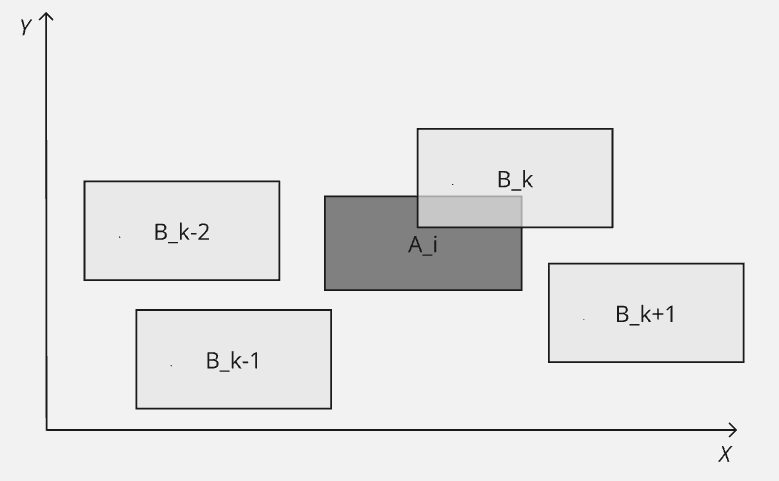
\includegraphics[width=0.75\linewidth]{figures/Optimazaciones/Interseccion/interseccion1a1.png}\par
    \caption{Ejemplificación de una iteración del proceso de intersección sobre dos conjuntos A y B.}
    \label{fig:int-graf}
\end{figure}

En algún punto, puede que se alcance un valor $k$, con $0 \leq k < \kappa(B)$, tal que el elemento mínimo de $B_k$ sea estrictamente mayor, en su primera dimensión (dimensión $0$), que el elemento máximo de $A_i$, tal como se muestra en la Figura~\ref{fig:criterio-parada}. Por ejemplo, si el mínimo de $B_k$ es $(3,5)$ y el máximo de $A_i$ es  $(2,3)$. En este caso, se pueden derivar las siguientes conclusiones:

\begin{itemize}
     \item La intersección entre $A_i$ y $B_k$ resulta vacía, ya que todos los valores de $A_i$ tienen un valor menor o igual que el máximo de $A_i$ en la primera dimensión y todos los valores de $B_k$ tienen un valor mayor o igual que el mínimo de $B_k$ en la primera dimensión.
    
    \item Debido al orden creciente de los conjuntos por el operador $<$ de multi-intervalos, cualquier multi-intervalo $B_{k'}$ con $k < k' < \kappa(B)$ tendrá en la primera dimensión de su mínimo un valor mayor o igual que el mínimo de $B_k$ en dicha dimensión, lo cual garantiza que también será vacía su intersección con $A_i$.
\end{itemize}

\begin{figure}[h]
    \centering
    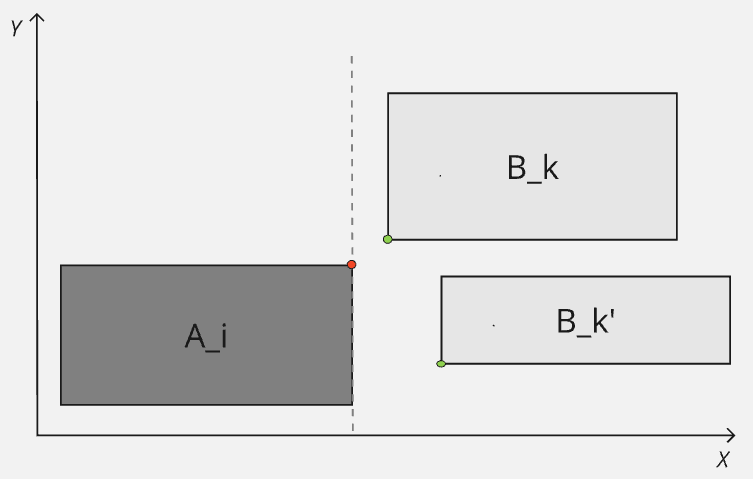
\includegraphics[width=0.75\linewidth]{figures/Optimazaciones/Interseccion/criterio de parada.png}
    \caption{Criterio de parada.}
    \label{fig:criterio-parada}
\end{figure}

En consecuencia, se puede establecer el siguiente criterio fundamental para optimizar la intersección entre conjuntos ordenados:

\begin{center}
    \fbox{
        \parbox{0.92\linewidth}{
            \centering
            \textbf{Criterio de parada} \\[1ex]
            \raggedright
            Sean $A$ y $B$ dos conjuntos ordenados. Supóngase que se está evaluando la intersección entre ambos, y en particular se consideran las posibles intersecciones entre un multi-intervalo $A_i$ de $A$, con $0 \leq i < \kappa(A)$, y los multi-intervalos de $B$. Dado un índice $k$ tal que $0 \leq k < \kappa(B)$, vale lo siguiente:

            \vspace{0,5cm}
     
            \textbf{Si} el máximo de $A_i$ es estrictamente menor que el mínimo de $B_k$ en la primera dimensión, \textbf{entonces}:

            \begin{itemize}
                \item la intersección entre $A_i$ y $B_{k'}$ resulta vacía, $\forall k' \mid k \leq k' < \kappa(B)$,
                \item \textbf{y, entonces} puede continuarse directamente con la evaluación de las intersecciones entre $A_{i+1}$(si existe) y los elementos de $B$.
            \end{itemize}
    
        }
    }
\end{center}

{\bf Criterio de eliminación}

\begin{center}
    \textit{Nuevamente, supóngase que se lleva a cabo la intersección entre $A$ y $B$, dos conjuntos ordenados, y se están considerando las posibles intersecciones del multi-intervalo \( i \)-ésimo de $A$, \( A_i \), con todos los multi-intervalos de $B$.}
\end{center}

En algún punto, puede que se alcance un valor $k$, con $0 \leq k < \kappa(B)$, tal que el elemento máximo de $B_k$ sea estrictamente menor, en su primera dimensión (dimensión $0$), que el elemento mínimo de $A_i$, tal como se muestra en la Figura~\ref{fig:criterio-eliminacion}. Por ejemplo, si el mínimo de $A_i$ es $(3,5)$ y el máximo de $B_k$ es  $(2,3)$. En este caso, se pueden derivar las siguientes conclusiones:

\begin{itemize}
     \item La intersección entre $A_i$ y $B_k$ resulta vacía, ya que todos los valores de $A_i$ tienen un valor mayor o igual que el mínimo de $A_i$ en la primera dimensión y todos los valores de $B_k$ tienen un valor menor o igual que el máximo de $B_k$ en la primera dimensión.

    \item Debido al orden creciente de los conjuntos por el operador $<$ de multi-intervalos, cualquier multi-intervalo $A_{i'}$ con $i < i' < \kappa(A)$ tendrá en la primera dimensión de su mínimo un valor mayor o igual que el mínimo de $A_i$ en dicha dimensión, lo cual garantiza que también será vacía su intersección con $B_k$.
\end{itemize}

\begin{figure}[h]
    \centering
    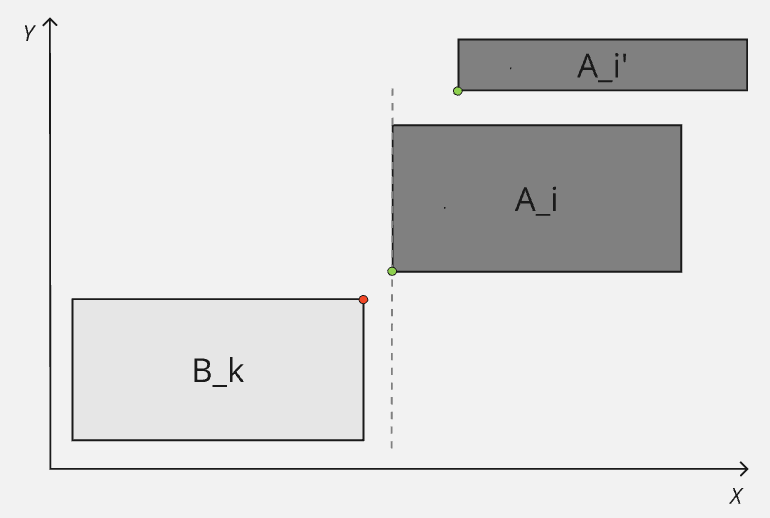
\includegraphics[width=0.75\linewidth]{figures/Optimazaciones/Interseccion/criterio de elim.png}
    \caption{Criterio de eliminación.}
    \label{fig:criterio-eliminacion}
\end{figure}

En consecuencia, se puede establecer el siguiente criterio fundamental para optimizar la intersección entre conjuntos ordenados:


\begin{center}
    \fbox{
        \parbox{0.92\linewidth}{
            \centering
            \textbf{Criterio de eliminación} \\[1ex]
            \raggedright
            Sean $A$ y $B$ dos conjuntos ordenados. Supóngase que se está evaluando la intersección entre ambos, y en particular se consideran las posibles intersecciones entre un multi-intervalo $A_i$ de $A$, con $0 \leq i < \kappa(A)$, y los multi-intervalos de $B$. Dado un índice $k$ tal que $0 \leq k < \kappa(B)$, vale lo siguiente:

            \vspace{0,5cm}
     
            \textbf{Si} el máximo de $B_k$ es estrictamente menor que el mínimo de $A_i$ en la primera dimensión, \textbf{entonces}:

            \begin{itemize}
                \item la intersección entre $A_{i'}$ y $B_{k}$ resulta vacía, $\forall i' \mid i \leq i' < \kappa(A)$,
                
                \item \textbf{y, entonces} puede descartarse $B_k$ para los cálculos de las posibles intersecciones de los multi-intervalos posteriores a $A_i$.
            \end{itemize}
    
        }
    }
\end{center}

Cabe señalar que, tanto para este criterio como para el anterior, no se especifica el tipo de multi-intervalo (si es denso o no), ya que dicha característica no afecta directamente la validez de los mismos.


{\bf Criterio de selección}

Tal como se analizó en el criterio de eliminación, el procedimiento de intersección considera cada multi-intervalo del conjunto $A$ e intenta intersectarlo con todos los multi-intervalos del conjunto $B$. Y donde la idea central del criterio es que, a medida que se avanza en este proceso, ciertos elementos de $B$ pueden ser descartados progresivamente si se determina que ya no podrán intersectar con los siguientes elementos de $A$.

Naturalmente, se puede llegar al punto en el cual todos los elementos de $B$ habrán sido descartados, lo que implica que la operación \texttt{intersection} podrá finalizar directamente ya que no quedan intersecciones posibles a verificar.

Ahora bien, existe una observación importante respecto al tamaño de $B$: cuanto menor sea la cantidad de multi-intervalos en $B$, más rápido podrán descartarse todos ellos posiblemente, y por tanto, terminar la operación.

En base a esta idea, se introduce el \textbf{criterio de selección}, el cual establece lo siguiente:

\begin{center}
    \fbox{
        \parbox{0.9\linewidth}{
            \centering
            \textbf{Criterio de selección} \\[1ex]
            \raggedright
            Sean dos conjuntos ordenados involucrados en la operación de intersección. Se establece lo siguiente:

            \begin{center}
            \textit{
                Se define como $B$ a aquel conjunto que contiene la menor cantidad de multi-intervalos,
                mientras que se denota como $A$ al conjunto restante.
            }
            \end{center}
        }
    }
\end{center}

{\bf Criterio de solapamiento}


Se introduce ahora el \textbf{criterio de solapamiento}, el cual establece lo siguiente:

\begin{center}
    \fbox{
        \parbox{0.93\linewidth}{
            \centering
            \textbf{Criterio de solapamiento} \\[1ex]
            \raggedright
            Sean $A$ y $B$ dos conjuntos, $A_i$ un multi-intervalo del conjunto $A$ y $B_k$ un multi-intervalo del conjunto $B$, con índices tales que:
            \[
            0 \leq i < \kappa(A), \quad 0 \leq k < \kappa(B).
            \]
            Se establece entonces que, en el caso de realizar la intersección entre $A$ y $B$:

            \begin{itemize}
                \item \textbf{Si} existe solapamiento entre $A_i$ y $B_k$, \textbf{entonces}:
                \begin{itemize}
                    \item \textbf{Si} ambos multi-intervalos son \textit{densos}, la intersección entre ellos es necesariamente no vacía y debe proceder.
                    \item \textbf{Si} al menos uno de ellos no es denso, la intersección \textit{puede} ser no vacía, pero no se garantiza de modo que se debe proceder de igual manera.
                \end{itemize}

                \item \textbf{Si} \textbf{no} existe solapamiento entre $A_i$ y $B_k$, \textbf{entonces} la intersección entre ellos es necesariamente vacía, independientemente de si son densos o no, y por ende puede obviarse su cálculo.
            \end{itemize}
        }
    }
\end{center}

Ahora bien, seguiría explicar que es el solapamiento en si:

\begin{center}
    \textit{Sean dos multi-intervalos $mdi_1$ y $mdi_2$. Los multi-intervalos $mdi_1$ y $mdi_2$ se \textbf{solapan} \textbf{si}, \textbf{y sólo si}, todos sus intervalos componentes en cada dimensión se solapan.}

    \textit{Sean $a = [a_{\text{begin}} : a_{\text{step}} : a_{\text{end}}]$ y $b = [b_{\text{begin}} : b_{\text{step}} : b_{\text{end}}]$ dos intervalos. Se dice que se \textbf{solapan} \textbf{si}, \textbf{y sólo si}, se cumple la siguiente condición:}

$\neg (b_{\text{end}} < a_{\text{begin}} \lor a_{\text{end}} < b_{\text{begin}})$

\textit{o bien las siguientes dos condiciones:}

$\bullet \;b_{\text{end}} \geq a_{\text{begin}}$ y $\bullet \;a_{\text{end}} \geq b_{\text{begin}}$

\end{center}

Para ejemplificar mejor la noción de solapamiento en intervalos se proponen los siguientes casos en base al predicado presentado por la definición:

\begin{itemize}
    \item \textbf{Caso $b_{\text{end}} < a_{\text{begin}}$ y $a_{\text{end}} \geq b_{\text{begin}}$:}

    En este caso, no hay solapamiento. Por ejemplo, si $b = [1:1:5]$ y $a = [6:2:10]$, entonces $5 < 6$, por lo tanto, no se solapan. Dicho ejemplo se puede ver en la Figura~\ref{fig:ej1}.

    \begin{figure}[h]
        \centering
        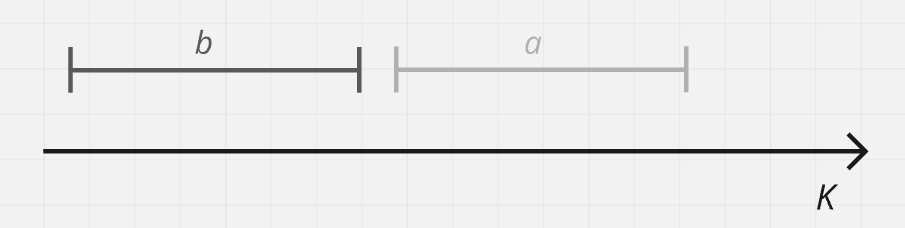
\includegraphics[width=0.75\linewidth]{figures/Optimazaciones/Interseccion/crit sol 10.png}
        \caption{Solapamiento sobre intervalos: \textit{segunda condición verdadera}.}
        \label{fig:ej1}
    \end{figure}

    \item \textbf{Caso $b_{\text{end}} \geq a_{\text{begin}}$ y $a_{\text{end}} < b_{\text{begin}}$:}

    Nuevamente, no hay solapamiento. Por ejemplo, si $b = [8:2:10]$ y $a = [4:2:6]$, entonces $6 < 8$. Este caso se puede observar en la Figura~\ref{fig:ej2}.

    \begin{figure}[h]
        \centering
        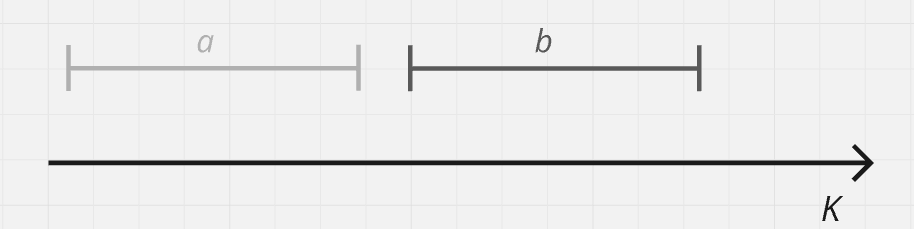
\includegraphics[width=0.75\linewidth]{figures/Optimazaciones/Interseccion/crit sol01.png}
        \caption{Solapamiento sobre intervalos: \textit{primera condición verdadera}.}
        \label{fig:ej2}
    \end{figure}

    \item \textbf{Caso ambas condiciones se cumplen:}

    En este caso resulta que se pueden dar dos situaciones unicamente: $b_{begin}$ o $b_{end}$ se encuentran entre $a_{begin}$ y $a_{end}$ inclusive (Figura~\ref{fig:crit-solapamiento-b}, Figura~\ref{fig:crit-solapamiento-c} y Figura~\ref{fig:crit-solapamiento-d}), ó $b_{begin} < a_{begin}$ y $b_{end}>a_{end}$ (Figura~\ref{fig:crit-solapamiento-a}).

\begin{figure}[H]
    \centering

    \begin{subfigure}{0.75\linewidth}
        \centering
        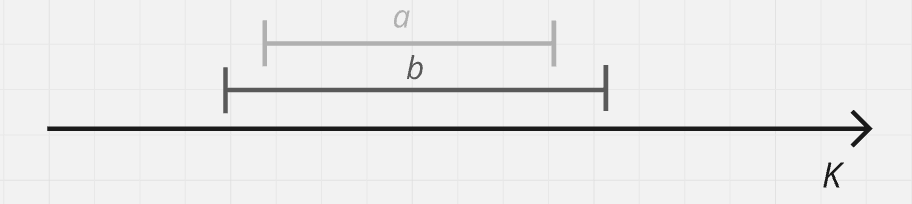
\includegraphics[width=\linewidth]{figures/Optimazaciones/Interseccion/crit sol 11 1.png}
        \caption{}
        \label{fig:crit-solapamiento-a}
    \end{subfigure}
    
    \vspace{0.4cm}

    \begin{subfigure}{0.75\linewidth}
        \centering
        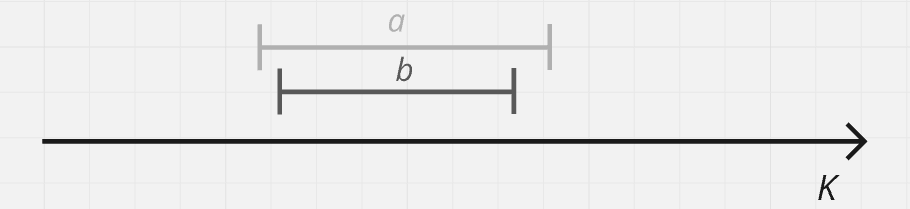
\includegraphics[width=\linewidth]{figures/Optimazaciones/Interseccion/crit sol 11 2.png}
        \caption{}
        \label{fig:crit-solapamiento-b}
    \end{subfigure}
    
    \vspace{0.4cm}

    \begin{subfigure}{0.75\linewidth}
        \centering
        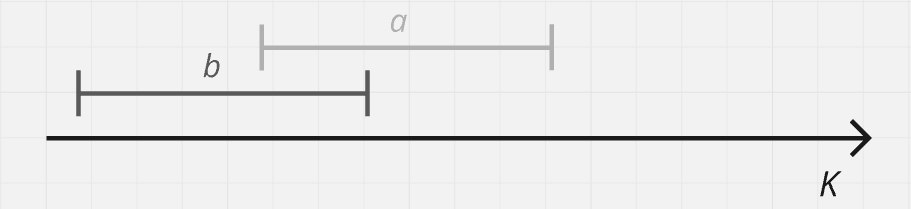
\includegraphics[width=\linewidth]{figures/Optimazaciones/Interseccion/crit sol 11 3.png}
        \caption{}
        \label{fig:crit-solapamiento-c}
    \end{subfigure}
    
    \vspace{0.4cm}

    \begin{subfigure}{0.75\linewidth}
        \centering
        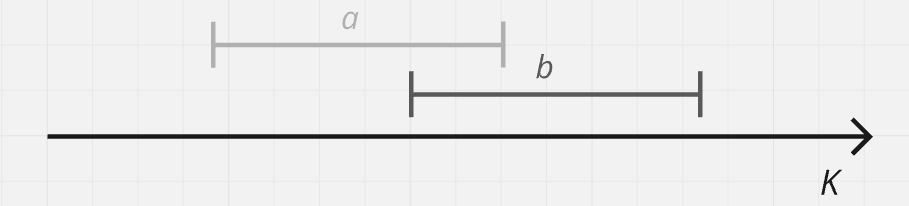
\includegraphics[width=\linewidth]{figures/Optimazaciones/Interseccion/crit sol 11 4.png}
        \caption{}
        \label{fig:crit-solapamiento-d}
    \end{subfigure}

    \caption{Solapamiento sobre intervalos: \textit{ambas condiciones se cumplen}.}
    \label{fig:crit-solapamiento}
\end{figure}
        \item \textbf{Caso ambas condiciones son falsas:}
        
        Cabe destacar que el caso en el cual \textbf{ambas condiciones} sean falsas simultáneamente es imposible. En efecto, si se cumple que:

        \[
        b_{\text{end}} < a_{\text{begin}} \quad \text{y} \quad a_{\text{end}} < b_{\text{begin}},
        \]
        
        entonces, por $a_{\text{begin}} < a_{\text{end}}$ y transitividad de la desigualdad, se deduce que:
        
        \[
        b_{\text{end}} < b_{\text{begin}},
        \]
        
        lo cual implicaría que el intervalo $b$ está mal definido, ya que su extremo final es menor que su extremo inicial. Esto contradice la definición válida de intervalo, por lo tanto, dicho caso \textbf{no} puede ocurrir.
\end{itemize}


Por un lado, se puede observar que si, en al menos una dimensión, los intervalos correspondientes de dos multi-intervalos $mdi$ y $mdi'$, ya sean densos o no, no se solapan, entonces no existe ninguna $n$-upla $(mdi[0], \dots, mdi[n-1]) \in mdi$ y $(mdi'[0], \dots, mdi'[n-1]) \in mdi'$ tal que coincidan en esa dimensión, con $n$ siendo la aridad de $mdi$ y $mdi'$. En consecuencia, esto implica que la intersección entre $mdi$ y $mdi'$ será vacía, independientemente de que en las demás dimensiones sí exista solapamiento.

Por otro lado, si en todas las dimensiones los intervalos correspondientes se solapan y ambos multi-intervalos son densos, entonces se garantiza la existencia de al menos una $n$-upla $(mdi[0], \dots, mdi[n-1])$ perteneciente tanto a $mdi$ como a $mdi'$.

Sin embargo, si uno o ambos multi-intervalos no son densos, esta garantía desaparece. Aunque exista solapamiento en todas las dimensiones, podría no haber ninguna $n$-upla común, ya que en alguna dimensión podría ocurrir que, debido al paso distinto de 1, el intervalo solapamiento puede no tener valores comunes. Por ejemplo, en una dimensión se pueden contar con los intervalos $[5:5:10]$ y $[6:1:9]$, los cuales se solapan, pero cuya intersección es vacía. 

\subsubsection{Criterio de ordenamiento}

Uno de los aspectos fundamentales a considerar al implementar la operación de intersección entre conjuntos ordenados, es cómo construir el conjunto resultado de manera que preserve el orden. En este contexto, el desafío consiste en insertar las intersecciones de los multi-intervalos en el conjunto resultado de la forma más eficiente posible, garantizando siempre que se mantenga la invariante del orden.

\begin{center}
    \fbox{
        \parbox{0.93\linewidth}{
            \centering
            \textbf{Criterio de ordenamiento} \\[1ex]
            \raggedright
            Supóngase que se realiza la intersección entre dos conjuntos ordenados, $A$ y $B$, y que se están evaluando las posibles intersecciones del $i$-ésimo multi-intervalo de $A$, denotado por $A_i$, con todos los multi-intervalos de $B$. Ademas se cuenta con un conjunto resultado $C$.

            \vspace{1ex}

            Todas las intersecciones no vacías generadas con $A_i$ deben insertarse en $C$ \textbf{después} de aquellas intersecciones generadas por los multi-intervalos $A_0, A_1, \dots, A_{i-1}$, cuyos mínimos sean estrictamente menores al de $A_i$, bajo el operador $<$ de naturales multi-dimensionales.
        }
    }
\end{center}


Este criterio se fundamenta en la observación de que la intersección entre dos multi-intervalos está contenida en ambos. Esto implica que el elemento mínimo de la intersección debe ser, necesariamente, un valor que pertenezca a ambos operandos, y por lo tanto debe coincidir con el mínimo de alguno de ellos, o bien ser un valor contenido en ambos.

Al fijar el multi-intervalo $A_i$ como decreta el criterio, se observa que cualquier intersección no vacía con un multi-intervalo $B_k$ del conjunto $B$ tendrá su mínimo dentro de $A_i$, o coincidirá con el mínimo de este. Como resultado, cualquier intersección no vacía generada tendrá un mínimo mayor, bajo el operador $<$ de naturales multi-dimensionales, o igual que el mínimo de $A_i$.

Esto garantiza que tales intersecciones deben insertarse en el conjunto resultado después de aquellas cuyo mínimo sea estrictamente menor, bajo el operador $<$ de naturales multi-dimensionales, al de $A_i$. 

La Figura~\ref{fig:enter-label} ilustra gráficamente esta situación. Como se observa, todas las intersecciones producidas a partir de $A_i$ tienen un mínimo mayor o igual que el de $A_i$, y se insertan a continuación de las intersecciones previamente procesadas cuyo mínimo sea menor al de $A_i$.

\begin{figure}[h]
    \centering
    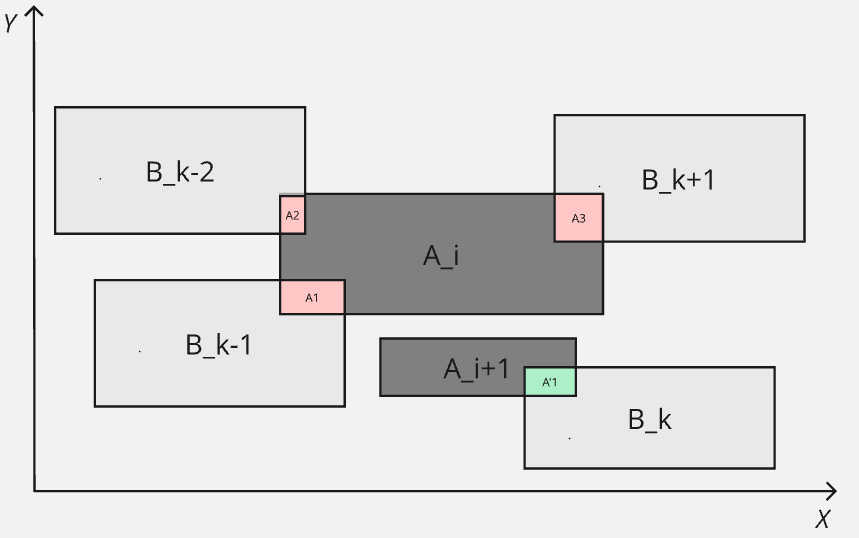
\includegraphics[width=0.7\linewidth]{figures/Optimazaciones/Interseccion/crit ordenamiento.png}
    \caption{Criterio de ordenamiento en la intersección de conjuntos ordenados.}
    \label{fig:enter-label}
\end{figure}

Adicionalmente, no es necesario comenzar a verificar la posición de inserción de las intersecciones en el conjunto resultado desde el principio en cada iteración de los elementos de $A$. Dado el orden intrínseco de los conjuntos involucrados, se cumple que:
\begin{center}
    \textit{El mínimo de $A_i$ es menor, bajo el operador $<$ de naturales multi-dimensionales, al mínimo de $A_{i+1}$}
\end{center}

Esto implica, en conjunto con lo establecido previamente sobre los mínimos de las intersecciones generadas, que todas las intersecciones obtenidas a partir de $A_{i+1}$ con los elementos de $B$ deben insertarse en el conjunto resultado a partir de una posición \textbf{igual o posterior} a aquella en la que comenzaron a insertarse las intersecciones de $A_i$ con $B$.

Por lo tanto, el criterio de ordenamiento puede refinarse del siguiente modo:



\begin{center}
    \fbox{
        \parbox{0.93\linewidth}{
            \centering
            \textbf{Criterio de ordenamiento} \\[1ex]
            \raggedright
            Supóngase que se realiza la intersección entre dos conjuntos ordenados, $A$ y $B$, y que se están evaluando las posibles intersecciones del $i$-ésimo multi-intervalo de $A$, denotado por $A_i$, con todos los multi-intervalos de $B$. Ademas se cuenta con un conjunto resultado $C$.

            \vspace{1ex}

            Todas las intersecciones no vacías generadas con $A_i$ deben insertarse en $C$ \textbf{después} de aquellas intersecciones generadas por los multi-intervalos $A_0, A_1, \dots, A_{i-1}$, cuyos mínimos sean estrictamente menores al de $A_i$, bajo el operador $<$ de naturales multi-dimensionales.
            
            \vspace{1ex}

            Adicionalmente \textbf{si} la posición a partir de la cual se colocan las intersecciones de $A_i$ en el conjunto resultante es $k$, con $0 \leq k < \kappa(C)$, \textbf{entonces} aquellas generadas por $A_{i+1}$ se insertaran a partir de $k'$ tal que $k \leq k' < \kappa(C)$.
        }
    }
\end{center}



Esta optimización reduce significativamente la cantidad de comparaciones necesarias para ubicar cada intersección, manteniendo la eficiencia del proceso y evitando retrocesos innecesarios dentro de la estructura del conjunto ordenado resultante.


\subsection{Unión disjunta - \texttt{disjointCup}}

La operación \texttt{disjointCup} se encarga de realizar la unión disjunta entre dos conjuntos de multi-intervalos que, por hipótesis, son disjuntos. En particular, esta operación simplemente coloca los elementos de ambos conjuntos en uno solo, sin aplicar ningún tipo de transformación adicional, ni sobre los argumentos, ni sobre el contenido de sus elementos. Esto se puede ver muy bien particularmente en el pseudocódigo del Algoritmo \ref{alg:disjointcupDes} de esta para conjuntos desordenados.

Ahora bien, al trabajar con conjuntos ordenados, resulta necesario introducir un criterio de ordenamiento que garantice que el conjunto resultante mantenga el orden. Este criterio de ordenamiento se presenta a continuación.

\subsubsection{Criterio de ordenamiento}

\begin{center}
    \fbox{
        \parbox{0.93\linewidth}{
            \centering
            \textbf{Criterio de ordenamiento}\\[1ex]
            \raggedright
            Sean $A = \{A_0, A_1, \dots, A_{n-1}\}$ y $B = \{B_0, B_1, \dots, B_{m-1}\}$ dos conjuntos no vacíos de multi-intervalos, disjuntos y ordenados. Sea $C$ un conjunto ordenado que contendrá el resultado de la fusión de $A$ y $B$. Y sean $A_i$ un multi-intervalo del conjunto $A$ y $B_k$ un multi-intervalo del conjunto $B$, con índices tales que:
            \[
            0 \leq i < \kappa(A), \quad 0 \leq k < \kappa(B).
            \]
            
            \vspace{1ex}

            Entonces, al realizar la unión disjunta entre $A$ y $B$ vale que:

            \begin{itemize}
                \item \textbf{Si $A_i < B_k$}, entonces $A_i$ debe insertarse en $C$ \textbf{antes} que $B_{k'}$ y $A_{i'}$, $\forall i',k' \mid i < i' < \kappa(A) \land k \leq k' < \kappa(B)$.
                \item \textbf{Si $B_k < A_i$}, entonces $B_k$ debe insertarse en $C$ \textbf{antes} que que $B_{k'}$ y $A_{i'}$, $\forall i',k' \mid i \leq i' < \kappa(A) \land k < k' < \kappa(B)$.
            \end{itemize}

            \vspace{1ex}
        }
    }
\end{center}

Este criterio se fundamente por el orden que disponen los conjuntos ordenados y a su vez por la propiedad transitiva que verifica el operador $<$ de multi-intervalos.

\subsection{Complemento - \texttt{complement / complementAtom}}

Esta sub-sección se dividirá en dos partes, ya que la operación de complemento para conjuntos ordenados, al igual que su contraparte de conjuntos desordenados, se compone de dos etapas: el \textit{complemento atómico} (\texttt{complementAtom}), que calcula el complemento de un conjunto ordenado representado por un único multi-intervalo; y el \textit{complemento general} (\texttt{complement}), la operación principal del complemento, que extiende esta operación tal que sea posible calcular el complemento de conjuntos ordenados compuestos por múltiples multi-intervalos sacando provecho de la operación \texttt{intersection}.

\subsubsection{Complemento atómico(\texttt{complementAtom})}

Dentro de la Sub-sección~\ref{sec:conjs-des} se presentó el funcionamiento y la lógica de la construcción del conjunto complemento de un conjunto atómico, un conjunto compuesto por un único multi-intervalo, mediante la operación \texttt{complementAtom}, en el contexto de los conjuntos desordenados.

Tal como se mencionó, la estructura general de la implementación de las operaciones para conjuntos ordenados se basa en la utilizada para conjuntos desordenados. Por esta razón, correspondería ahora optimizar dicha operación teniendo en cuenta el orden y adaptarla para conjuntos ordenados.

Sin embargo, dado que el conjunto base contiene únicamente un multi-intervalo y solo se cuenta con un único conjunto como argumento de la operación, no hay margen para aplicar ninguna optimización basada en el orden de los argumentos de entrada. 

Por lo tanto, la única tarea pendiente es mantener el orden en el resultado, lo cual implica determinar el \textbf{criterio de ordenamiento}.

{\bf Criterio de ordenamiento}

En \texttt{complementAtom} se trabaja con dos tipos de multi-intervalos: \textit{all} y \textit{during}. Las transformaciones sucesivas de estos intervalos conforman el complemento del conjunto atómico. El uso de cada uno es el siguiente:

Sea $i$ un número natural que hace referencia una dimensión entre $0$ y la cantidad de dimensiones del conjunto atómico procesado.
\begin{itemize}
  \item \textbf{\textit{all}}:  
    Construye el multi-intervalo ($\textit{all}_{i,b}$) que va desde $0$ hasta el inicio del multi-intervalo del conjunto en la dimensión $i$, siempre que exista.

  \item \textbf{\textit{during}}:  
    Cuando el multi-intervalo del conjunto no es denso en la dimensión $i$, es decir, el paso de la $i$-esima dimensión ($\text{paso}_i$) es distinto de $1$, se generan una serie de multi-intervalos intermedios ($\textit{during}_{i,c}$). Cada uno arranca en
    \[
      \bigl(\text{begin}_i\bigr) + c,
      \quad c = 1, 2, \dots, (\text{paso}_i - 1),
    \]
    donde $\text{begin}_i$ es el inicio en la dimensión $i$ del multi-intervalo del conjunto.

  \item \textbf{\textit{all}}:  
    Construye el multi-intervalo ($\textit{all}_{i,e}$) que va desde el final del multi-intervalo del conjunto en la dimensión $i$ hasta \texttt{Inf}, siempre que sea posible.
\end{itemize}

Sin embargo, al realizar el procesamiento secuencial de cada dimensión, es necesario tener en cuenta cómo los inicios de los intervalos correspondientes a las dimensiones ya recorridas del multi-intervalo  se propagan hacia $all$ y $during$. 

Una vez completados los cálculos en la dimensión $i$ (creación de \textit{all}$_{i,b}$, \textit{all}$_{i,e}$ y todos los \textit{during}$_{i,c}$), tanto \textit{during} como \textit{all} se modifican en dicha dimensión. A \textit{all} se le remplaza el intervalo en esa dimensión por el del multi-intervalo del conjunto en la misma dimensión pero con paso 1, y a \textit{during} se le hace lo mismo pero con el intervalo original.

Como consecuencia, todos los multi-intervalos que se generen en la siguiente dimensión $i+1$ tienen el mismo valor de inicio en la dimensión $i$ que tiene el multi-intervalo del conjunto. Por lo tanto los inicios de \textit{all}$_{i,b}$, \textit{all}$_{i,e}$ y de cada \textit{during}$_{i,c}$ coinciden, en las dimensiones $0,1,\ldots,i-1$, con los del multi-intervalo atómico original. Lo que conlleva a que el siguiente conjunto este ordenado:

\[
\{\textit{all}_{i,b},\;\textit{during}_{i,1},\;\textit{during}_{i,2},\;\dots,\;\textit{during}_{i,k},\;\textit{all}_{i,e}\}
\]

Pero ahora queda ver que interacción hay entre los conjuntos de cada dimensión para ver como ordenar la totalidad de los multi-intervalos de todas las dimensiones en un único conjunto.

Al estar en una dimensión $i$ y al haber terminado de generar los multi-intervalos de esa dimensión a través de \textit{during} y \textit{all}, por como son las modificaciones a estos dos multi-intervalos, resulta que todos los multi-intervalos generados en la dimensión $i+1$ van inmediatamente después de $all_{i,b}$(si existe), ya que en la dimensión $i$ tiene un valor de inicio $0$. Ademas, se los debe incluir antes de los \textit{during}$_{i,c}$, cuyo inicio en la dimensión $i$ es el mismo que el de los multi-intervalos generados en $i+1$, adicionando una constante $c$. Como resultado tenemos que se da el siguiente orden:

\begin{align*}
\{ &\textit{all}_{x,b},\ \textit{all}_{y,b},\ \textit{all}_{z,b}, \\
   &\textit{during}_{z,1},\ \textit{during}_{z,2},\ \dots,\ \textit{during}_{z,k}, \\
   &\textit{all}_{z,e},\ \textit{during}_{y,1},\ \textit{during}_{y,2},\ \dots,\ \textit{during}_{y,j}, \\
   &\textit{all}_{y,e},\ \textit{during}_{x,1},\ \textit{during}_{x,2},\ \dots,\ \textit{during}_{x,j}, \\
   &\textit{all}_{x,e} \}
\end{align*}

trabajando con un conjunto atómico de tres dimensiones.

A partir de todo lo analizado previamente, se arriba a la siguiente formulación del criterio de ordenamiento para \texttt{complementAtom}:

\begin{center}
    \fbox{
        \parbox{0.93\linewidth}{
            \centering
            \textbf{Criterio de ordenamiento}\\[1ex]
            \raggedright
            El patrón general de inserción en las estructuras auxiliares $all$ y $during$, al recorrer las dimensiones en orden creciente, responde a la siguiente disposición:

            \begin{align*}
            \{ &\textit{all}_{0,b},\ \textit{all}_{1,b},\ \dots,\ \textit{all}_{k-1,b}, \\
               &\textit{during}_{k-1,1},\ \dots,\ \textit{during}_{k-1,u_{i-1}}, \\
               &\textit{all}_{k-1,e},\ \textit{during}_{k-2,1},\ \dots,\ \textit{during}_{k-2,u_{i-2}}, \\
               &\quad\vdots \\
               &\textit{all}_{1,e},\ \textit{during}_{0,1},\ \dots,\ \textit{during}_{0,u_0}, \\
               &\textit{all}_{0,e} \}
            \end{align*}

            \vspace{1ex}

            donde $k$ representa la aridad del conjunto (es decir, la cantidad de dimensiones), y $u_i$ indica la cantidad de pasos definidos en la dimensión $i$.
        }
    }
\end{center}



\subsubsection{Complemento general}

La operación \texttt{intersection} se utiliza como herramienta para calcular el complemento entre dos conjuntos desordenados en la operación \texttt{complement}: uno que representa el complemento de un conjunto de multi-intervalos desordenados, y otro que representa el complemento de un conjunto con un único multi-intervalo.

Teóricamente, podría utilizarse una única implementación general de \texttt{intersection}, como se hace en el caso de conjuntos desordenados y no modificar \texttt{complement} para el caso de conjuntos ordenados. Sin embargo, al tratarse de conjuntos ordenados, es posible aplicar ciertas optimizaciones adicionales, además de algunas de las ya detalladas en la sub-sección correspondiente a \texttt{intersection}, que permiten mejorar el rendimiento de la operación. Es decir, se utilizará una versión adaptada de la intersección de conjuntos ordenados para el complemento.

{\bf Intersección complementaria}

En esta modificación de la operación de intersección, denominada \texttt{intersectionComp}, se preservan los criterios de \textbf{solapamiento} y \textbf{ordenamiento}. Además de suponer que los conjuntos recibidos están ordenados, esta variante introduce una hipótesis adicional: los argumentos deben respetar un orden específico. El primer conjunto debe representar el complemento de un conjunto de multi-intervalos (posiblemente varios), mientras que el segundo conjunto corresponde al complemento de un único multi-intervalo. 

En otras palabras:
\begin{itemize}
    \item El primer conjunto, $A$, actúa como un \emph{complemento acumulado}.
    \item El segundo conjunto, denotado $B$, funciona como un \emph{complemento unitario}.
\end{itemize}

\textbf{Importante:} Para facilitar la siguiente explicación, se asume que los multi-intervalos involucrados son siempre densos.

Supongase ahora que el conjunto $A$ representa el complemento de un único multi-intervalo, al igual que $B$. Esta situación se ilustra en la Figura~\ref{fig:tra}.

\begin{figure}[htbp]
    \centering
    \begin{minipage}[t]{0.49\textwidth}
        \centering
        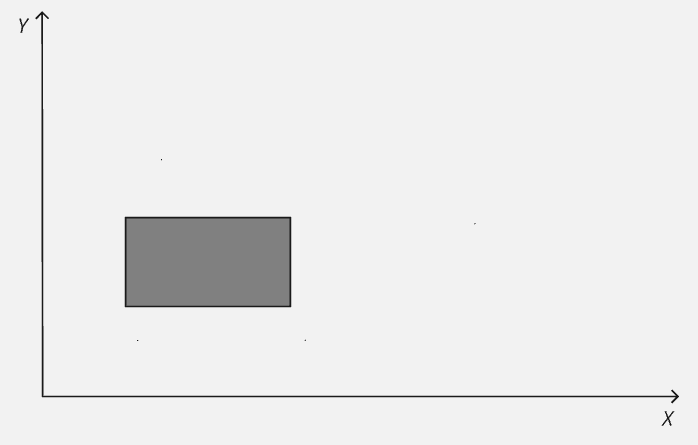
\includegraphics[width=\linewidth]{figures/Optimazaciones/Complement/Aelem.png}
        \caption*{\small Multi-intervalo generador de $A$}
        \vspace{8pt}
        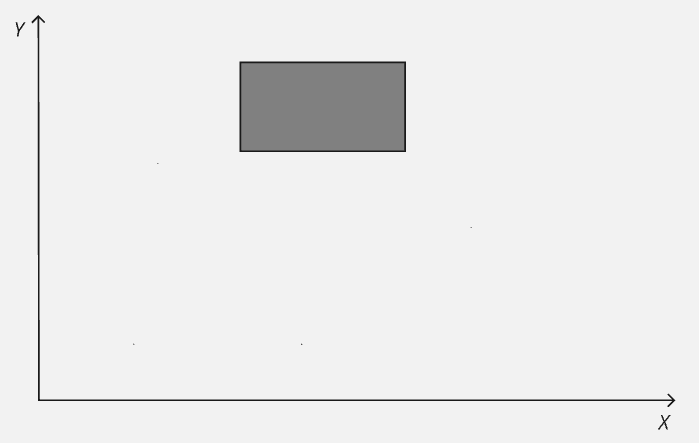
\includegraphics[width=\linewidth]{figures/Optimazaciones/Complement/Belem.png}
        \caption*{\small Multi-intervalo generador de $B$}
    \end{minipage}%
    \hspace{0.01\textwidth}
    \begin{minipage}[t]{0.49\textwidth}
        \centering
        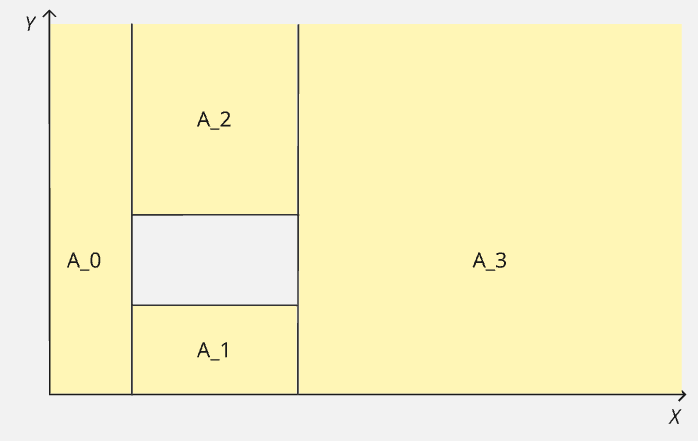
\includegraphics[width=\linewidth]{figures/Optimazaciones/Complement/A.png}
        \caption*{\small Conjunto complemento $A$}
        \vspace{8pt}
        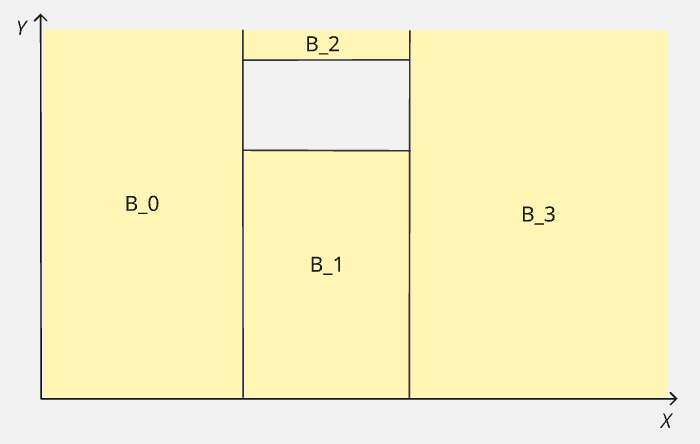
\includegraphics[width=\linewidth]{figures/Optimazaciones/Complement/B.png}
        \caption*{\small Conjunto complemento $B$}
    \end{minipage}
    \caption{Ejemplo gráfico de los conjuntos complemento de $A$ y $B$.}
    \label{fig:tra}
\end{figure}

Si se aplicara directamente la operación \texttt{intersection}, utilizando su versión optimizada para conjuntos ordenados, el resultado obtenido sería el ilustrado en la Figura~\ref{fig:compleAnt}. 

Sin embargo, puede observarse que se produce una partición adicional innecesaria: los multi-intervalos $C\_1$ y $C\_3$ podrían haberse mantenido como un único multi-intervalo. Esta fragmentación/particionamiento es consecuencia del funcionamiento de la operación intersección. No obstante, ambos multi-intervalos no comparten ningún elemento con el multi-intervalo generador de $B$, por lo que no deberían verse afectados ni sufrir ninguna sustracción de elementos al quitar de $A$ los elementos del multi-intervalo generador de $B$ a través de la intersección de $A$ y $B$.


\begin{figure}[htbp]
    \centering
    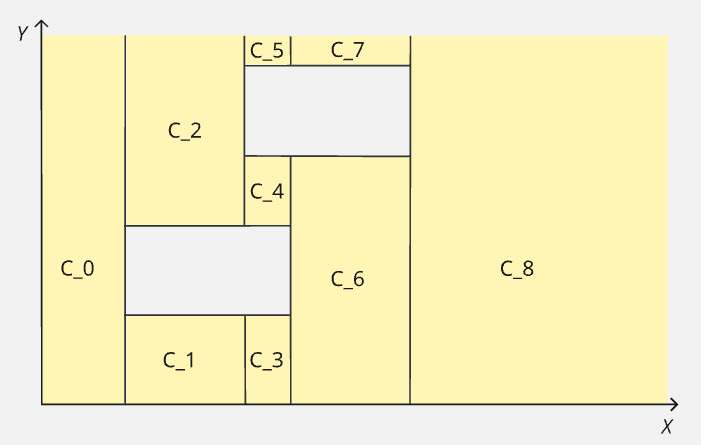
\includegraphics[width=0.8\linewidth]{figures/Optimazaciones/Complement/complAnt.png}
    \caption{Conjunto complemento resultante de la intersección entre $A$ y $B$, sin aplicar optimización.}
    \label{fig:compleAnt}
\end{figure}

Este tipo de fragmentación innecesaria puede evitarse mediante el criterio de optimización denominado \textbf{criterio de anti-particionamiento}, que establece lo siguiente:

\begin{center}
    \fbox{
        \parbox{0.93\linewidth}{
            \centering
            \textbf{Criterio de anti-particionamiento} \\[1ex]
            \raggedright
            Sea $A$ un conjunto complemento y $B$ el complemento de un conjunto compuesto por un único multi-intervalo $mdi$. Al realizar la intersección entre $A$ y $B$ durante el cálculo del complemento de un conjunto, se cumple que:
            
            \vspace{1ex}
            Todo multi-intervalo de $A$ que no se solape con el multi-intervalo $mdi$ generado por $B$ no requiere ser intersectado con los elementos de $B$, y debe copiarse directamente al conjunto resultado.
        }
    }
\end{center}


Aplicando este criterio, el conjunto complemento resultante se muestra en la Figura~\ref{fig:compleNue}, donde se observa una representación más compacta: se evita una partición innecesaria y se obtiene un conjunto más chico.

\begin{figure}[htbp]
    \centering
    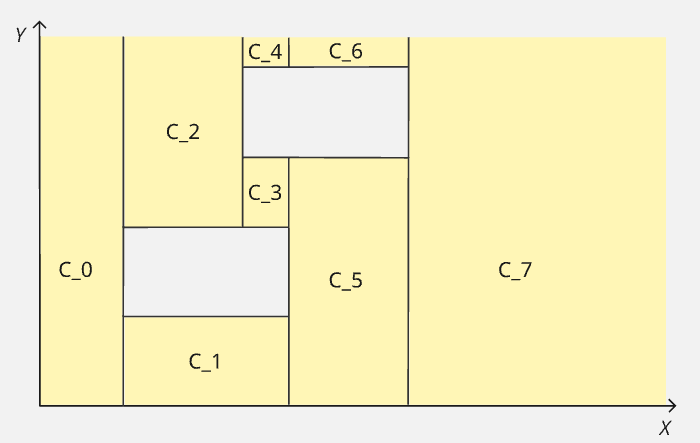
\includegraphics[width=0.8\linewidth]{figures/Optimazaciones/Complement/complNue.png}
    \caption{Conjunto complemento resultante tras aplicar el criterio de anti-particionamiento.}
    \label{fig:compleNue}
\end{figure}

Cabe destacar que este criterio también es válido cuando se trabaja con multi-intervalos no densos, y resulta especialmente útil en esos casos, ya que evita múltiples operaciones de posicionamiento y comparación innecesarias.

Si bien la reducción en el número de multi-intervalos resultantes puede parecer ínfima, es importante tener en cuenta que en la operación \texttt{complement} se aplica de forma acumulativa esta reducción. Por lo tanto, reducir la cantidad de particiones en cada iteración tiene un efecto significativo en el rendimiento total, ya que disminuye la cantidad de elementos a recorrer y comparar en las iteraciones posteriores.

Existe además una mejora adicional que puede aplicarse a la operación de intersección en el contexto del complemento. Esta surge por el modo en que se construye el complemento ordenado de un conjunto atómico, tal como se explicó en la subsección correspondiente del complemento atómico.

En dicha construcción, el primer multi-intervalo del complemento ordenado es $\textit{all}_{x,b}$. Este multi-intervalo es denso y se extiende hasta el infinito en todas sus dimensiones, con excepción de la primera, donde finaliza una posición antes del comienzo del multi-intervalo original que dio lugar al complemento.

Adicionalmente se cumple que la intersección entre cualquier multi-intervalo y uno denso, que lo contiene por completo, es simplemente el multi-intervalo contenido. Es decir, si un multi-intervalo $mdi$ está completamente contenido en otro multi-intervalo denso $mdi'$, entonces la intersección entre $mdi$ y $mdi'$ es igual a $mdi$.

A partir de las observaciones anteriores, puede establecerse el criterio de optimización denominado \textbf{criterio de obviedad}, el cual permite evitar cálculos innecesarios durante la intersección del complemento, y estipula lo siguiente:

\begin{center}
    \fbox{
        \parbox{0.93\linewidth}{
            \centering
            \textbf{Criterio de obviedad} \\[1ex]
            \raggedright
            Sea $A$ un conjunto complemento y $B$ el complemento de un conjunto compuesto por un único multi-intervalo $mdi$. Al realizar la intersección entre $A$ y $B$ durante el cálculo del complemento de un conjunto, se cumple que:

            \vspace{0,5cm}
            
            Todo multi-intervalo del conjunto $A$ cuyo máximo sea estrictamente menor en la primera dimensión que el mínimo multi-intervalo generador de $B$, $mdi$, puede incorporarse directamente al conjunto resultado de la intersección, sin necesidad de ser intersectado con los elementos de $B$.
        }
    }
\end{center}


\begin{comment}
    

\begin{figure}[htbp]
    \centering
    \begin{minipage}[t]{0.49\textwidth}
        \centering
        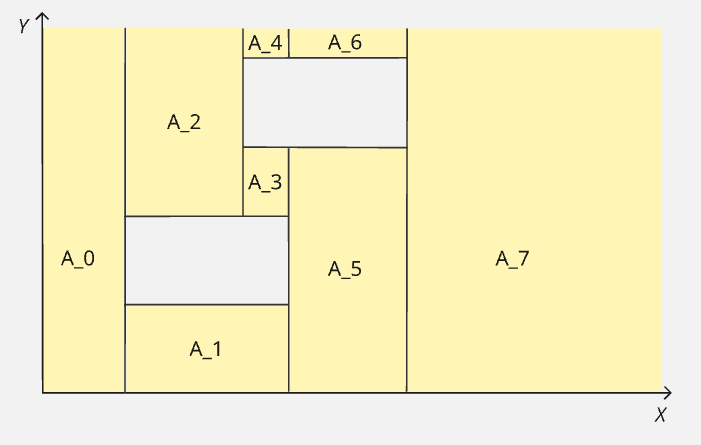
\includegraphics[width=\linewidth]{figures/Optimazaciones/Complement/Ao.png}
        \caption*{\small Conjunto complemento $A$}
    \end{minipage}%
    \hspace{0.01\textwidth}
    \begin{minipage}[t]{0.49\textwidth}
        \centering
        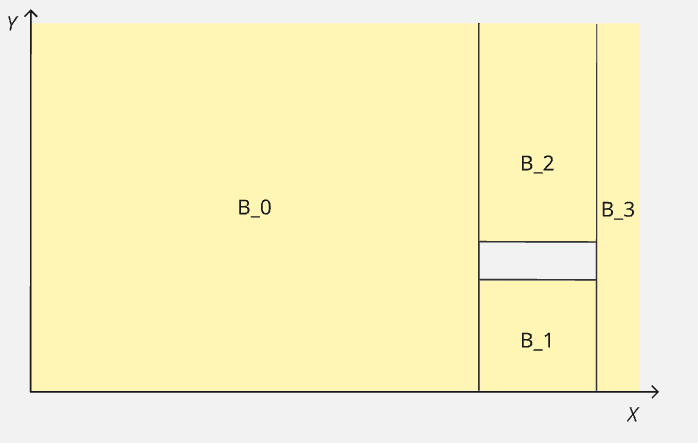
\includegraphics[width=\linewidth]{figures/Optimazaciones/Complement/Bo.png}
        \caption*{\small Conjunto complemento $B$}
    \end{minipage}
    \hspace{0.01\textwidth}
    \begin{minipage}[t]{0.49\textwidth}
        \centering
        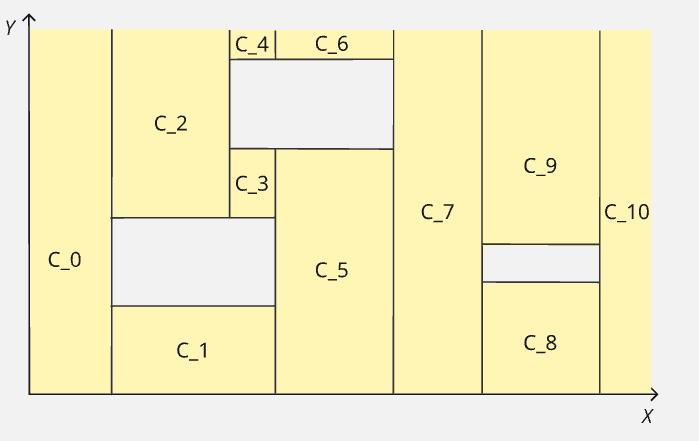
\includegraphics[width=\linewidth]{figures/Optimazaciones/Complement/complO.png}
        \caption*{\small Conjunto complemento resultante de la intersección}
    \end{minipage}
    \caption{Ejemplo gráfico de los conjuntos complemento $A$ y $B$.}
    \label{fig:tra}
\end{figure} 
\end{comment}


Tal como fue planteado, el \textbf{criterio de obviedad} permite evitar las comparaciones e intersecciones entre determinados multi-intervalos del conjunto complemento $A$ y los elementos del conjunto complemento $B$, pero su alcance inicial es limitado: únicamente evita el procesamiento de los multi-intervalos de $A$ que sean estrictamente menores (en la primera dimensión) que el multi-intervalo generador de $B$ en una única invocación de la operación \texttt{intersectionComplement}.

Sin embargo, este criterio puede extenderse de forma significativa durante el proceso iterativo de la operación \texttt{complement}. Esto es posible gracias a la siguiente observación: los multi-intervalos que generan cada conjunto $B$ a lo largo de las distintas iteraciones provienen de un conjunto ordenado, por lo tanto, sus valores iniciales en la primera dimensión son no decrecientes. Dado que estos multi-intervalos se recorren en orden, cada nuevo multi-intervalo generador $B$ tendrá en la primera dimensión un valor de inicio igual o mayor que el anterior. Y, por ende cada nuevo $\textit{all}_{x,b}$ del conjunto $B$ generado por un multi-intervalo contendrá a todos los anteriores $\textit{all}_{x,b}$.

Como consecuencia, una vez que un multi-intervalo de $A$ ha sido descartado por el criterio de obviedad en una iteración, puede descartarse definitivamente para todas las iteraciones subsiguientes, ya que siempre será obviado por el criterio obviedad.

Esto permite trasladar dichos multi-intervalos directamente al resultado final de la operación \texttt{complement}, en lugar de seguirlos incorporando los en el cálculo de las posteriores iteraciones.

Se procede entonces a declarar el \textbf{criterio de obviedad extendido}:

\vspace{10pt}

\begin{center}
    \fbox{
        \parbox{0.93\linewidth}{
            \centering
            \textbf{Criterio de obviedad extendido} \\[1ex]
            \raggedright
            Sea $A$ un conjunto ordenado de multi-intervalos que representa el complemento acumulado en una iteración de la operación \texttt{complement} y $B$ el complemento de un conjunto compuesto por un único multi-intervalo de dicha iteración también.

            \vspace{0,5cm}
            
            Entonces, $A$ puede \textit{descomponerse} en dos subconjuntos disjuntos:
            \begin{itemize}
                \item $A\_o$: el subconjunto de multi-intervalos que son descartados por el criterio de obviedad en base a $B$ en dicha iteración, y que, por lo tanto, pueden ser incorporados directamente al resultado final sin necesidad de ser procesados en iteraciones posteriores;

                
                \item $A\_r$: el subconjunto restante, compuesto por los multi-intervalos que aún pueden ser particionados en iteraciones futuras, es decir, aquellos que no son descartados por el criterio de obviedad en base a $B$. Luego, la intersección se dará entre este conjunto y $B$, y su resultado será el nuevo $A$.
            \end{itemize}
        }
    }
\end{center}

Este criterio permite ahorrar el recorrer los mismos elementos múltiples veces durante el calculo de la intersección e el complemento. Esto permite aumentar en gran medida la eficiencia de la operación.

\section{Implementaciones}

Para llevar a cabo la implementación de los conjuntos ordenados, fue necesario desarrollar una serie de funciones adicionales. A continuación, se describen dichas implementaciones complementarias junto con su correspondiente pseudocódigo.

\subsection{Calculo de solapamiento - \texttt{doInt}}

La operación \texttt{doInt} se utiliza en el contexto de conjuntos ordenados, aunque no forma parte de su interfaz de operaciones. Esta tiene el objetivo de calcular si existe solapamiento entre dos multi-intervalos. Esta operación resulta fundamental tanto para la aplicación del \textbf{criterio de solapamiento} como para el \textbf{criterio de anti-particionamiento}.

El pseudocódigo correspondiente a esta operación se presenta a continuación, y resulta relativamente breve:


\begin{algorithm}
\caption{Cálculo de solapamiento para conjuntos ordenados}
\begin{algorithmic}[1]
\Require $Mdi\_1$ y $Mdi\_2$ son dos multi-intervalos
\Ensure Devuelve \texttt{true} si estos se solapan, \texttt{false} en caso contrario.
\Function{doInt}{$Mdi\_1, Mdi\_2$}

    \
    
    \State $max\_1 :=$ \Call{maxElem}{$Mdi\_1$}
    \State $min\_1 :=$ \Call{minElem}{$Mdi\_1$}
    \State $max\_2 :=$ \Call{maxElem}{$Mdi\_2$}
    \State $min\_2 :=$ \Call{minElem}{$Mdi\_2$}
    \State $a :=$ \Call{arity}{$Mdi\_1$}

    \

    \For{$i = 0$; $i < a-1$ ; $i \!+\!+$}
         \If{$max\_1[i] < min\_2[i]$ \textbf{or} $max\_2[i] < min\_1[i]$}
            \State \Return \texttt{false} 
        \EndIf
    \EndFor

    \
    
    \State \Return \texttt{true} 

\EndFunction
\end{algorithmic}
\end{algorithm}

\subsection{Inserción con pista - \texttt{emplaceHint}}

La función \texttt{emplaceHint} se propone también como una herramienta auxiliar externa a la estructura principal de conjuntos ordenados. Su tarea consiste en insertar un multi-intervalo en un conjunto ordenado, siguiendo el mismo criterio de ordenamiento utilizado por los mismos. Para hacerlo, utiliza una posición pista (\textit{hint}), es un número natural y una posición sugerida y que sirve como punto de inicio para encontrar eficientemente la ubicación correcta del multi-intervalo.

El pseudocódigo de esta función es corto, ya que su implementación es simple, y se encuentra en el Algoritmo \ref{alg:emplaceHint-conj}.

\begin{algorithm}
\caption{Inserción con pista para conjuntos ordenados}
\label{alg:emplaceHint-conj}
\begin{algorithmic}[1]
\Require $A$ es una conjunto ordenado, $Mdi$ en un multi-intervalo y $Hint$ es un numero natural y una posición sugerida.
\Ensure Inserta el $Mdi$ dentro del conjunto ordenado, manteniendo el orden y empezando a buscar la posición de inserción a partir de $Hint$.
\Function{emplaceHint}{$A,Mdi,Hint$}
     \State $n :=$ \Call{size}{$A$}
    \State $it := Hint$ 
    \While{$it < n$}
        \If{$A_{it} < mdi$}
            \State $it$ \!+\!+
        \Else
            \State \textbf{break}
        \EndIf
    \EndWhile

      \State $A :=$ $A_{0:it-1} \frown \{mdi\} \frown A_{it:\Call{size}{A}-1}$
\EndFunction
\end{algorithmic}
\end{algorithm}


\subsection{Avance con pista - \texttt{advanceHint}}

La función \texttt{advanceHint} se propone también como una herramienta auxiliar externa a la estructura principal de conjuntos ordenados. El objetivo de esta función es avanzar la posición de la pista (hint) que viene como argumento en función de los elementos presentes en un conjunto ordenado, utilizando un multi-intervalo como criterio de parada.

El pseudocódigo de esta función auxiliar se presenta a continuación.


\begin{algorithm}
\caption{Avance con pista para conjuntos ordenados}
\label{alg:advanceHint}
\begin{algorithmic}[1]
\Require $A$ es un conjunto ordenado, $Mdi$ en un multi-intervalo y $Hint$ es un número natural.
\Ensure Avanza la pista $Hint$ en base a los elementos del conjunto y el $Mdi$.
\Function{advanceHint}{$A,Mdi,Hint$}
    \State $n :=$ \Call{size}{$A$}
    
    \While{$Hint < n$}
        \If{$A_{Hint} < Mdi$}
            \State $Hint$ \!+\!+
        \Else
            \State \textbf{break}
        \EndIf
    \EndWhile
\EndFunction
\end{algorithmic}
\end{algorithm}



\section{Implementaciones}

Llegado este punto, es momento de abordar las implementaciones concretas de las distintas operaciones sobre conjuntos ordenados. 

Esta seccion se organiza en tres sub-secciones principales: una dedicada a aquellas operaciones cuya implementación no requirió modificaciones, una sub-sección que aborda las operaciones adaptadas para poder funcionar correctamente en el contexto de conjuntos ordenados, y finalmente otra correspondiente a las operaciones que fueron optimizadas.

\subsection{Operaciones sin cambios}

Al implementar los conjuntos ordenados utilizando como base la versión desordenada, se observó que ciertas operaciones no podían beneficiarse del orden para su optimización o no se podían optimizar en si, pero tampoco alteraban dicho orden. Esto se debe, principalmente, a dos razones: o bien son operaciones que no devuelven un conjunto ordenado, o bien el conjunto resultante ya se encuentra ordenado.

Dentro del primer conjunto de operaciones se incluyen, por ejemplo: \texttt{cardinal}, que devuelve el número de elementos que contiene el conjunto; \texttt{arity}, que informa la aridad del mismo; entre otras.

Dado que estas operaciones son numerosas y su comportamiento no resulta central para los objetivos de esta tesina, además de que sus implementaciones se mantuvieron sin modificaciones, no se detallarán aquí. Todas ellas pueden consultarse en el archivo \textit{set.cpp}, disponible en el repositorio dentro de la carpeta \textit{sbg}.

En el segundo conjunto se incluyen operaciones como \texttt{compact}, cuyo algoritmo no elimina el orden del conjunto resultante, o \texttt{cup}, cuya lógica interna se basa exclusivamente en operaciones que preservan dicho orden.

Al igual que en el caso anterior, se omite un desarrollo mas amplio de estas operaciones. Si se desea consultarlas en profundidad puede dirigirse al archivo \textit{set.cpp}, disponible en el repositorio dentro de la carpeta \textit{sbg}.

\subsection{Operaciones adaptadas al orden}

Este grupo de operaciones fueron adaptadas para funcionar en el contexto de conjuntos ordenados, pero no pudieron ser optimizadas. Dentro de estas operaciones se encuentran:

\begin{itemize}
    \item \texttt{emplace}: Que se encarga de ubicar un multi-intervalo dentro de un conjunto.
    \item \texttt{emplaceBack}: Que se encarga de ubicar un multi-intervalo al final de un conjunto, como su último elemento, aquel con mayor mínimo.
    \item \texttt{minElem}: Busca el mínimo mínimo de todos los multi-intervalos de un conjunto
\end{itemize}

Si se desea ver cuales fueron sus modificaciones con respecto a sus versiones de conjuntos desordenados, puede verifica el archivo \textit{set.cpp} dentro de la carpeta \textit{sbg}, disponible en el repositorio.

\subsection{Operaciones optimizadas}

En esta sub-sección se presentan aquellas operaciones que pudieron ser optimizadas aprovechando el orden de los conjuntos. Cada una de ellas será descripta minuciosamente y explicada en detalle, destacando los criterios de optimización y ordenamiento en cada caso.

\subsubsection{Intersección - \texttt{intersection}}
Como se puede observar a continuación, la operación \texttt{intersection} resultó ser considerablemente más extensa que su homóloga para conjuntos desordenados.

No obstante, teniendo en cuenta lo expuesto en la Sub-sección~\ref{sec:opts-int}, se tiene lo siguiente:

\begin{itemize}
    \item Para implementar el \textbf{criterio de selección}, se realiza la verificación correspondiente según lo establecido por dicho criterio: se analiza la cantidad de multi-intervalos presentes en los conjuntos $C$ y $D$. A partir de esta comparación, se determina cuál es el conjunto largo, $A$, y cuál el corto, $B$, tal como se muestra en el Algoritmo \ref{alg:int-ord-1}, líneas 12 a 17.

    \item En relación con el \textbf{criterio de eliminación}, dado que su cumplimiento implica la remoción de un elemento de uno de los conjuntos, en este caso del conjunto $B$, y dado que no es posible eliminar elementos directamente del mismo, se utiliza una lista enlazada que contiene los índices que referencian a los multi-intervalos de $B$. Esto permite llevar a cabo la eliminación de los índices en vez de los multi-intervalos. La preparación de dicha lista se observa en el Algoritmo \ref{alg:int-ord-1}, líneas 18 a 21, y la implementación del criterio se detalla en el Algoritmo \ref{alg:int-ord-2}, líneas 7 a 10.

    \item En cuanto el \textbf{criterio de parada} este se implementa de la linea 11 a 13 en el Algoritmo \ref{alg:int-ord-2}, donde lo único que se hace es forzar la salida del segundo bucle a través de un \texttt{break}.

    \item Para la aplicación del \textbf{criterio de solapamiento}, se emplea la función auxiliar \texttt{doInt}, encargada de verificar si dos multi-intervalos se solapan. Esto se encuentra en el Algoritmo \ref{alg:int-ord-2}, línea 14.

    \item Finalmente, el \textbf{criterio de ordenamiento} se implementa mediante las funciones auxiliares \texttt{advanceHint} y \texttt{emplaceHint}, permitiendo que al aplicar el criterio, el conjunto resultado se mantenga ordenado a lo largo de la ejecución. Esto puede observarse en el Algoritmo \ref{alg:int-ord-2}, líneas 3 y 17.
\end{itemize}

\begin{algorithm}
\caption{Intersección de conjuntos ordenados — Parte 1: Preparación}\label{alg:int-ord-1}
\begin{algorithmic}[1]
\Require $C$ y $D$ son conjuntos ordenados
\Ensure $R$ es la intersección ordenada de $C$ y $D$
\Function{intersection}{$C, D$}
    \State $R := \{\}$

    \If{$\Call{isEmpty}{C}$ \textbf{or} $\Call{isEmpty}{D}$}
        \State \Return{$R$}
    \EndIf

    \If{$C == D$}
        \State \Return{$C$}
    \EndIf
 
    
    \If{ \Call{maxElem}{$C$} $<$ \Call{minElem}{$D$} $ $\textbf{or}$ $ \Call{maxElem}{$C$} $<$ \Call{minElem}{$D$} }
        \State \Return{$R$}
    \EndIf

    
    \State $B := C$
    \State $A := D$

    \If{\Call{size}{$D$} $<$ \Call{size}{$C$}}
        \State $B := D$
        \State $A := C$
    \EndIf

    \State $indices := []$ \Comment{Es una lista simplemente enlazada}
    \For{$i = 0$; $i < \Call{size}{B}$; $i$ \!+\!+ }
        \State $indices := indices$  \!+\!+  $[i]$ \Comment{Se concatenan las listas enlazadas}
    \EndFor

    
    \State $r\_pos := 0$
\EndFunction
\end{algorithmic}
\end{algorithm}


\begin{algorithm}
\caption{Intersección de conjuntos ordenados — Parte 2: Construcción del resultado}\label{alg:int-ord-2}
\begin{algorithmic}[1]
\Function{intersection}{}
    \ForAll{$a \in A$}
        \State $\Call{advanceHint}{R,a,r\_pos}$

        \State $i := 0$
                
        \While{$i \neq \Call{length}{indices}$}
                
            \State $b := B_{indices[i]}$
            \If{\Call{maxElem}{$a$}[0] $<$ \Call{minElem}{$b$}[0]}
                \State $indices := indices 	\triangleleft  i$
                \State \textbf{continue}
            \EndIf

            \If{\Call{maxElem}{$a$}[0] $<$ \Call{minElem}{$b$}[0]}
                \State \textbf{break}
            \EndIf
            \If{\Call{doInt}{$b$,$a$}}
                \State $inter :=$ \Call{intersection}{$a, b$}
                \If{$\neg \Call{isEmpty}{inter}$}
                    \State $\Call{emplaceHint}{R,inter,r\_pos}$
                \EndIf
            \EndIf
    
            \State $i$ \!+\!+ 
        \EndWhile
        
        \If{$indices == []$}
            \State \textbf{break}
        \EndIf
    \EndFor
    \State \Return{$R$}
\EndFunction
\end{algorithmic}
\end{algorithm}



\newpage
\subsubsection{Unión disjunta - \textit{disjointCup}}

A continuación se presenta el pseudocódigo correspondiente a la implementación de la operación \texttt{disjointCup}, encargada de llevar a cabo la unión disjunta de conjuntos ordenados. 

El algoritmo de fusión que implementa la unión disjunta debe recorre entonces ambos conjuntos en paralelo: tomando el indice $i\_a$ para $A$ y $i\_b$ para $B$, comenzando ambos en 0. En cada iteración de la operación se aplica el \textbf{criterio de ordenamiento}. El procedimiento distingue los siguientes casos:

\begin{itemize}
    \item \textbf{Si $A_{i\_a} < B_{i\_b}$}: se agrega $A_{i\_a}$ al final de $C$ y se incrementa el índice ${i\_a}$ (i.e., $i\_a$\!+\!+ ).
    \item \textbf{En caso contrario} (es decir, $A_i \geq B_{i\_b}$): se agrega $B_{i\_b}$ al final de $C$ y se incrementa el índice $i\_b$ (i.e., $i\_b$\!+\!+ ).
\end{itemize}

Este proceso se repite hasta que al menos uno de los dos conjuntos ($A$ o $B$) haya sido recorrido completamente. Una vez alcanzado ese punto, se agregan al final de $C$ todos los elementos restantes del conjunto que aún no se haya agotado, preservando su orden original.

La Figura~\ref{fig:unionDis-ejemplo} ejemplifica el proceso de ejecución de la función \texttt{disjointCup}. En ella, los multi-intervalos de los conjuntos $A$ y $B$ están representados respectivamente en rojo y verde cuando son sometidos al criterio de ordenamiento. Estos elementos pasan a través del criterio de ordenamiento definido, determinando su incorporación al conjunto resultante $C$, cuyos elementos se muestran en amarillo a medida que se insertan.


\begin{figure}[htbp]
\hspace{-0.06\textwidth} % Desplaza toda la figura hacia la izquierda
\begin{minipage}{0.49\textwidth}
    \centering
    \subgraphics{figures/Optimazaciones/traverse/crir ordenameitno (1).png}{}%
    \vspace{4pt}

    \subgraphics{figures/Optimazaciones/traverse/crir ordenameitno (2).png}{}%
    \vspace{4pt}

    \subgraphics{figures/Optimazaciones/traverse/crir ordenameitno (3).png}{}%
    \vspace{4pt}

    \subgraphics{figures/Optimazaciones/traverse/crir ordenameitno (4).png}{}
\end{minipage}%
\hspace{0.01\textwidth} % Ajusta el espacio entre las columnas
\begin{minipage}{0.49\textwidth}
    \centering
    \subgraphics{figures/Optimazaciones/traverse/crir ordenameitno (5).png}{}%
    \vspace{4pt}

    \subgraphics{figures/Optimazaciones/traverse/crir ordenameitno (6).png}{}%
    \vspace{4pt}

    \subgraphics{figures/Optimazaciones/traverse/crir ordenameitno (7).png}{}%
    \vspace{4pt}

    \subgraphics{figures/Optimazaciones/traverse/crir ordenameitno (8).png}{}
\end{minipage}
\caption{Ilustración del criterio de ordenamiento aplicado en la fusión \texttt{disjointCup} dado un conjunto $A$ y $B$ ordenados y disjuntos.}
\label{fig:unionDis-ejemplo}
\end{figure}







\begin{algorithm}
\caption{Unión de conjuntos ordenados disjuntos}\label{alg:two}
\begin{algorithmic}[1]
\Require $A$ y $B$ son conjuntos ordenados
\Ensure $C$ es la unión disjunta ordenada de $A$ y $B$
\Function{disjointCup}{$A,B$}

\If{$\Call{isEmpty}{A}$}
    \State \Return $B$
\EndIf
\If{$\Call{isEmpty}{B}$}
    \State \Return $A$
\EndIf

\State $C  := \{\}$
\State $i\_a  := 0$
\State $i\_b  := 0$
\State $end\_a :=$ \Call{size}{$A$}
\State $end\_b :=$ \Call{size}{$B$}


\If{\Call{minElem}{$A_{end\_a - 1}$} $<$ \Call{minElem}{$B_0$}}
    \State \Return $A \frown B$
\EndIf

\If{\Call{minElem}{$B_{end\_b - 1}$} $<$ \Call{minElem}{$A_0$}}
    \State \Return $B \frown A$
\EndIf

\For{;$i\_a \neq end\_a$ \textbf{and} $i\_b \neq end\_b$;}
  \If{$A_{i\_a} < B_{i\_b}$} 
    \State \Call{emplaceBack}{$C$, $A_{i\_a}$}
    \State $i\_a$ \!+\!+
  \Else 
    \State \Call{emplaceBack}{$C$, $B_{i\_b}$}
    \State $i\_b$ \!+\!+
  \EndIf   
\EndFor


\State $C := C \frown A_{i\_a:end\_a - 1}$
\State $C := C \frown B_{i\_b:end\_b - 1}$

\State \Return $C$
\EndFunction
\end{algorithmic}
\end{algorithm}

\newpage

\begin{comment}
    

\section{OrderedSets - cup}

En el caso de la operación \texttt{cup}, puede observarse que no se han introducido cambios con respecto a su versión homóloga utilizada para conjuntos desordenados. Esta coincidencia no es casual, sino que responde directamente a la forma en que dicha operación ha sido definida. Este diseño permite reutilizar la lógica sin necesidad de adaptaciones adicionales, lo cual representa una ventaja en términos de simplicidad y consistencia del código.

\begin{algorithm}
\caption{Unión de conjuntos ordenados (posible intersección)}\label{alg:unionGeneral}
\begin{algorithmic}[1]
\Require $A$ y $B$ son conjuntos ordenados
\Ensure El resultado es la unión ordenada de $A$ y $B$
\Function{cup}{$A,B$}

\

\If{$A == \emptyset$}
    \State \Return $B$
\EndIf
\If{$B == \emptyset$ \textbf{or} $A == B$}
    \State \Return $A$
\EndIf

\

\If{\Call{maxElem}{$A$} $<$ \Call{minElem}{$B$}}
    \State \Return $A \frown B$
\EndIf

\If{\Call{maxElem}{$B$} $<$ \Call{minElem}{$A$}}
    \State \Return $B \frown A$
\EndIf

\

\State $D :=$ \Call{difference}{$B$, $A$} 
\State \Return \Call{disjointCup}{$B$, $D$}
\EndFunction
\end{algorithmic}
\end{algorithm}


\newpage
\section{OrderedSets - difference}

Al igual que la operación \texttt{cup}, la operación \texttt{difference} no presenta modificaciones específicas respecto a su versión implementada con conjuntos desordenados. Por este motivo, cualquier mejora en su rendimiento proviene exclusivamente de las optimizaciones aplicadas a las operaciones subyacentes que utiliza.


\begin{algorithm}
\caption{Diferencia de conjuntos ordenados}\label{alg:two}
\begin{algorithmic}[1]
\Require $A$ y $B$ son conjuntos ordenados
\Ensure El resultado es la diferencia ordenada de $A$ con $B$
\Function{difference}{$A,B$}

\ 

\If{$A == \emptyset$ \textbf{or} $B == \emptyset$}
    \State \Return $\emptyset$
\EndIf

\

\If{\Call{maxElem}{$A$} $<$ \Call{minElem}{$B$}}
    \State \Return $A$
\EndIf

\If{\Call{maxElem}{$B$} $<$ \Call{minElem}{$A$}}
    \State \Return $A$
\EndIf

\

\State $D :=$ \Call{complement}{$B$}
\State \Return \Call{intersection}{$A$, $D$}
\EndFunction
\end{algorithmic}
\end{algorithm}

\newpage
\end{comment}


\subsubsection{Complemento - \texttt{complement}}

A continuación se presenta el pseudocódigo correspondiente a la implementación de la operación \texttt{complement} en el Algoritmo \ref{alg:complement-conj-ord}, la cual es similar a su homóloga para conjuntos desordenados. 

La única diferencia significativa radica en la incorporación parcial del \textbf{criterio de obviedad extendido}, generando un conjunto ordenado de multi-intervalos obviados $R$, que se pasa como argumento a la operación \texttt{intersectionComp}. En esta es donde se realizará la división de $A$ en los dos subconjuntos disjuntos que se mencionan en el criterio. 

Este proceso puede observarse en las líneas 6 y 16, respectivamente.


\begin{algorithm}
\caption{Complemento de conjuntos ordenados}\label{alg:complement-conj-ord}
\begin{algorithmic}[1]
\Require $A$ es un conjunto ordenado
\Ensure El resultado es el complemento ordenado de $A$
\Function{complement}{$C$}

\If{$\Call{isEmpty}{C}$}
    \State \Return $ \{\}$
\EndIf

\State $A :=  \{\}$
\State $R :=  \{\}$

\State $first\_mdi := A_0$
\State $A :=$ \Call{complementAtom}{$\{first\_mdi\}$}

\For{$i=1$; $i \neq \Call{size}{C}$ ; $i$ \!+\!+}
    \State $mdi := C_i$
    \State $atomic\_set :=$ \Call{complementAtom}{$\{mdi\}$}
    \State $A :=$ \Call{intersectionComp}{$A, atomic\_set,R,mdi$}
\EndFor

\State \Return \Call{disjointCup}{$R$, $A$}
\EndFunction
\end{algorithmic}
\end{algorithm}


\newpage
\subsubsection{Complemento atómico - \texttt{complementAtom}}

En lo que respecta a la operación \texttt{complementAtom}, esta debía mantenerse equivalente a su contraparte para conjuntos desordenados, pero incorporando el \textbf{criterio de ordenamiento} definido específicamente para esta operación.

Como se puede observar en el pseudocódigo a continuación, dicho criterio se implementa mediante el uso de las variables numéricas $pos\_global$ y $pos\_local$ (línea 15 en el Algoritmo~\ref{alg:complementAtom-part1} y línea 3 en el Algoritmo~\ref{alg:complementAtom-part2}), así como a través de la colocación ordenada de los elementos dentro del conjunto de salida $C$, en las líneas 10, 24 y 35 en el Algoritmo~\ref{alg:complementAtom-part2}.

\begin{algorithm}
\caption{Complemento atómico para conjuntos ordenados — Parte 1: Preparación}\label{alg:complementAtom-part1}
\begin{algorithmic}[1]
\Require $A$ es un conjunto ordenado atómico
\Ensure $D$ es el complemento ordenado de $A$
\Function{complementAtom}{$A$}

  \State $C := \{\}$  
  \State $mdi := A_0$  
  \State $dense\_mdi := []$

  \ForAll{$interval \in mdi$}
    \State $b :=$ \Call{begin}{$interval$}
    \State $e :=$ \Call{end}{$interval$}
    \State \Call{emplaceBack}{$dense\_mdi, [b : 1 : e]$}
  \EndFor

  \State $during\_mdi := dense\_mdi$
  \State $univ := [0:1:\texttt{Inf}]$
  \State $a :=$ \Call{arity}{$A$}
  \State $all := univ^a$ \Comment{Universo de dimensión $a$}

  \State $dim := 0$
  \State $pos\_global := 0$
\EndFunction
\end{algorithmic}
\end{algorithm}

\begin{algorithm}
\caption{Complemento atómico para conjuntos ordenados— Parte 2: Construcción y retorno}\label{alg:complementAtom-part2}
\begin{algorithmic}[1]
\Function{complementAtom}{}
  \ForAll{$i \in mdi$}
    \State $pos\_local := pos\_global$
    \State $b :=$ \Call{begin}{$i$}


    \If{\Call{begin}{$i$} $\neq 0$}
      \State $i\_res := [0:1:$ \Call{begin}{$i$}$-1]$
      \If{$\neg \Call{isEmpty}{i\_res}$}
        \State $all[dim] := i\_res$
        \State $n :=$ \Call{size}{$C$}
        \State $C := C_{0:pos\_local - 1} \frown \{all\} \frown C_{pos\_local:n - 1}$
        \State $pos\_local$ \!+\!+, \, $pos\_global$ \!+\!+
        \State $all[dim] := univ$
      \EndIf
    \EndIf

    \If{\Call{begin}{$i$} $<$ \texttt{Inf}}
        \If{\Call{step}{$i$} $> 1$}
          \For{$j = 0$; $j < size(A)$; $j$\!+\!+}
            \State $h := [$\Call{begin}{$i$}$ + j + 1 : $\Call{step}{$i$} $: $ \Call{end}{$i$}$]$
            \If{$\neg \Call{isEmpty}{h}$}
              \State $during\_mdi[dim] := h$
              \State $n :=$ \Call{size}{$C$}
              \State $C := C_{0: pos\_local - 1} \frown \{during\_mdi\} \frown C_{pos\_local:n - 1}$
              \State $pos\_local$ \!+\!+
            \EndIf
          \EndFor
        \EndIf
    \EndIf

    \If{\Call{end}{$i$} $<$ \texttt{Inf}}
      \State $i\_res := [$\Call{end}{$i$}$+1 : 1 : \texttt{inf}]$
      \If{$\neg \Call{isEmpty}{i\_res}$}
        \State $all[dim] := i\_res$
        \State $n :=$ \Call{size}{$C$}
        \State $C := C_{0:pos\_local - 1} \frown \{all\} \frown C_{pos\_local:n - 1}$
        \State $pos\_local \!+\!+$
        \State $all_{dim} := univ$
      \EndIf
    \EndIf

    \State $all[dim] := dense\_mdi[dim]$
    \State $during\_mdi[dim] := i$
    \State $dim$ \!+\!+
  \EndFor

  \State \Return $C$
\EndFunction
\end{algorithmic}
\end{algorithm}


\newpage
\subsubsection{Intersección complementaria - \texttt{intersectionComp}}

Por último, se presenta la operación adicional \texttt{intersectionComp}, la cual permite calcular una intersección optimizada cuando se ejecuta la operación \texttt{complement}.

Cabe recordar que esta operación es una variante de la operación \texttt{intersection} presentada anteriormente. Sin embargo, a diferencia de aquella, \texttt{intersectionComp} solo implementa el \textbf{criterio de solapamiento} y el \textbf{criterio de ordenamiento}, y, ademas, incorpora los tres criterios de optimización adicionales vistos con anterioridad:

\begin{itemize}
    \item Se implementa el \textbf{criterio de obviedad} y la parte faltante del \textbf{criterio de obviedad extendido}, ambos utilizando el multi-intervalo $Mdi$ . Esto puede observarse en el Algoritmo~\ref{alg:int-comp-1}, líneas 10 a 13 del pseudocódigo, donde se subdivide a $A$ en $Remnant$ y $A_{pos:\Call{size}{A}}$, que tienen los elementos que ya forman parte del resultado final del complemento y los elementos restantes a interseccionar, respectivamente.

    \item En cuanto al \textbf{criterio de anti-particionamiento} en el Algoritmo~\ref{alg:int-comp-2}, se lleva a cabo mediante el uso de la función auxiliar \texttt{doInt}, que permite realizar un chequeo de solapamiento entre los multi-intervalos de $A$, y los de $B$. En función de este resultado, se decide si realizar el recorrido por los elementos de $B$, o bien guardar directamente los multi-intervalos de $A$ en el conjunto resultado.
\end{itemize}

\begin{algorithm}
\caption{Intersección complementaria para conjuntos ordenados — Parte 1: Preparación}
\label{alg:int-comp-1}
\begin{algorithmic}[1]
\Require $A$ y $B$ son conjuntos ordenados, $Remnant$ un conjunto ordenado, y $Mdi$ un multi-intervalo
\Ensure $C$ es la intersección ordenada de los elementos necesarios $A$ y $B$
\Function{intersectionComp}{$A, B, Remnant, Mdi$}
    \State $C := \{\}$
    
    \If{\Call{isEmpty}{$A$} \textbf{or} \Call{isEmpty}{$B$}}
        \State \Return $C$
    \EndIf

    \If{$A == B$}
        \State \Return $A$
    \EndIf

    \ 
    
    \State $pos := 0$
    
    \While{$pos <$ \text{\Call{size}{$A$}} \textbf{and} \Call{maxElem}{$A_{pos}$}[0] $<$ \Call{minElem}{$Mdi$}[0]}
        \State \Call{emplaceBack}{$Remnant, A_{pos}$}
        \State $pos$ \!+\!+
    \EndWhile

    
    \ 
    
    \State $c\_pos := 0$
\EndFunction
\end{algorithmic}
\end{algorithm}


\begin{algorithm}
\caption{Intersección complementaria para conjuntos ordenados — Parte 2: Construcción del resultado}
\label{alg:int-comp-2}
\begin{algorithmic}[1]
\Function{intersectionComp}{}
\State $endA :=$ \text{\Call{size}{$A$}}
    \ForAll{$a \in  A_{pos:endA-1}$}
        \State $do\_int :=$ \Call{doInt}{$a, mdi$}
        \State $\Call{advanceHint}{C, a, c\_pos}$
    

    \ 
    
        \If{$do\_int$}
            \ForAll{$b \in B$}        
            \If{\Call{doInt}{$b$,$a$}}
                \State $inter :=$ \Call{intersection}{$a, b$}
                \If{$\neg$ \Call{isEmpty}{$inter$}}
                    \State \Call{emplaceHint}{$C$,$inter$,$c\_pos$}
                \EndIf
            \EndIf
        
    
            \EndFor
   \
        
        \Else
            \State \Call{emplaceHint}{$C, a, c\_pos$}
        \EndIf
        
    \
    

    \EndFor
            
    \
    
    \State \Return{$C$}
\EndFunction
\end{algorithmic}
\end{algorithm}
\chapter{\textit{Piecewise maps} ordenados}

De manera análoga a lo realizado con los \textbf{conjuntos ordenados}, 
se introducen ahora los \textbf{\textit{Piecewise maps} ordenados}. 
El objetivo de este capítulo es explicar cómo estos almacenan los mapas, 
presentar las optimizaciones obtenidas, \textit{criterios de optimización} y criterios de ordenamiento, y finalmente, detallar la forma en que 
dichas optimizaciones fueron incorporadas en las operaciones de los \textit{Piecewise maps} ordenados.

\section{Estructura y orden}

Ahora es el turno de los \textbf{\textit{piecewise maps} ordenados}. A diferencia de los conjuntos ordenados, no se disponía de una implementación previa que ofreciera una estructura ordenada de ninguna índole, capaz de brindar pistas de cómo desarrollar el criterio de orden. En consecuencia, fue necesario desarrollar dicho criterio desde cero.

Inicialmente, los piecewise maps ordenados deben contar con una variable miembro que contenga los mapas que se desean almacenar. Esta variable se denominará \texttt{pieces\_}, aunque por el momento no se le asignará un tipo concreto, ya que primero es necesario definir el criterio de orden.

El objetivo es construir un criterio de orden que permita reutilizar y aprovechar los conceptos desarrollados para optimizar los conjuntos ordenados, aun cuando ahora se trabaja con mapas. Recordemos que un \texttt{Map} está definido por las siguientes dos componentes:

\begin{itemize}
  \item Un conjunto dominio;
  \item Una colección de expresiones lineales.
\end{itemize}

Se decidió tomar como base del criterio de orden a los conjuntos dominio, ya que estos están definidos en base a los multi-intervalos, y pueden ayudar a cumplir el objetivo planteado anteriormente. En cambio, las expresiones lineales no aportan ninguna ventaja aparente, por lo cual son descartadas para gestionar el orden dentro de los \textit{piecewise maps} ordenados.

Definido el elemento sobre el cual se va a basar el orden, corresponde establecer cuándo un mapa se considera estrictamente menor que otro:

\begin{center}
Sean $m_1 = dom_1 \longmapsto exps_1$ y $m_2 = dom_2 \longmapsto exps_2$ dos mapas arbitrarios, es decir, objetos de tipo \texttt{Map}. \\
Entonces, se define que $m_1 < m_2$ si y solo si $minPer_1 < minPer_2$, \\
donde la comparación se realiza con el operador $<$ de los naturales multi-dimensionales o \texttt{MD\_NAT}, y $minPer_1$ y $minPer_2$ son los mínimos perimetrales de $dom_1$ y $dom_2$, respectivamente.
\end{center}

Ahora bien, el mínimo perimetral se define de la siguiente manera:

\begin{center}
Sea $x = (x_0, x_1, \dots, x_{n-1})$ un natural multi-dimensional o \texttt{MD\_NAT}, y sea $C$ un conjunto. \\
Entonces, $m$ es el \textbf{mínimo perimetral} de $C$ si para todo $j \in \{0, \dots, k-1\}$ se cumple que $x_j$ es el mínimo valor en la $j$-ésima dimensión entre todos los elementos de $C$.

\textbf{Por ejemplo:} Considerando el conjunto $C = \{mdi_1,mdi_2,mdi_3\}$, siendo $mdi_1 =$ $[2:1:2]\times[3:2:9]$, $mdi_2 =$ $[1:1:2]\times[5:2:9]$ y $mdi_3 =$ $[2:1:2]\times[1:2:9]$, el mínimo perimetral seria $(1,1)$. 
\end{center}

Teniendo todo esto presente, y dado que los conjuntos no implementan ningún método que permita calcular el mínimo perimetral, la idea será generar una operación adicional para calcular dicho mínimo, realizar esa operación una única vez (ya que implica recorrer todos los mínimos de un conjunto), y almacenarlo junto con su mapa correspondiente. 

En consecuencia, la variable \texttt{pieces\_} tendrá la siguiente forma:

\[
\texttt{pieces\_} = \ll (m_0,\ minPer_0),\ (m_1,\ minPer_1),\ \dots,\ (m_{k-1},\ minPer_{k-1}) \gg
\]

donde para todo $i, j \in \{0,\dots,k-1\}$ con $i < j$, se cumple que $m_i < m_j$, es decir, $minPer_i < minPer_j$.

Con esto, el orden dentro de un \textit{piecewise map} ordenado queda definido. Sin embargo, esto no es suficiente para aprovechar por completo los conceptos utilizados para optimizar los conjuntos ordenados. Para ello, es necesario definir también el concepto de \textbf{máximo perimetral}:

\begin{center}
Sea $x = (x_0, x_1, \dots, x_{n-1})$ un natural multi-dimensional o \texttt{MD\_NAT}, y sea $C$ un conjunto. \\
Entonces, $m$ es el \textbf{máximo perimetral} de $C$ si para todo $j \in \{0, \dots, k-1\}$ se cumple que $x_j$ es el máximo valor en la $j$-ésima dimensión entre todos los elementos de $C$.

\textbf{Por ejemplo:} Considerando el conjunto $C = \{mdi_1,mdi_2,mdi_3\}$, siendo $mdi_1$, $mdi_2$ y $mdi_3$ los dados en el ejemplo anterior, el máximo perimetral seria $(2,9)$. 
\end{center}

Esta información también debe ser almacenada, tal como se hizo con el mínimo perimetral. Por lo tanto, la variable \texttt{pieces\_} tendrá ahora la siguiente estructura extendida:


\begin{align*}
\texttt{pieces} = \ll \, 
  & (m_0,\ (\texttt{minPer}_0,\ \texttt{maxPer}_0)), \\
  & (m_1,\ (\texttt{minPer}_1,\ \texttt{maxPer}_1)), \\
  & \dots, \\
  & (m_{k-1},\ (\texttt{minPer}_{k-1},\ \texttt{maxPer}_{k-1})) \,\gg
\end{align*}



Este concepto funciona como contraparte del mínimo perimetral y permite interpretar el conjunto dominio de un mapa como si fuera un único multi-intervalo definido por su mínimo y su máximo perimetral. En la Figura~\ref{fig:minmaxPer1} se muestra un ejemplo de esta interpretación de manera gráfica, donde dicho multi-intervalo está marcado en línea punteada.

\begin{figure}[ht]
  \centering
  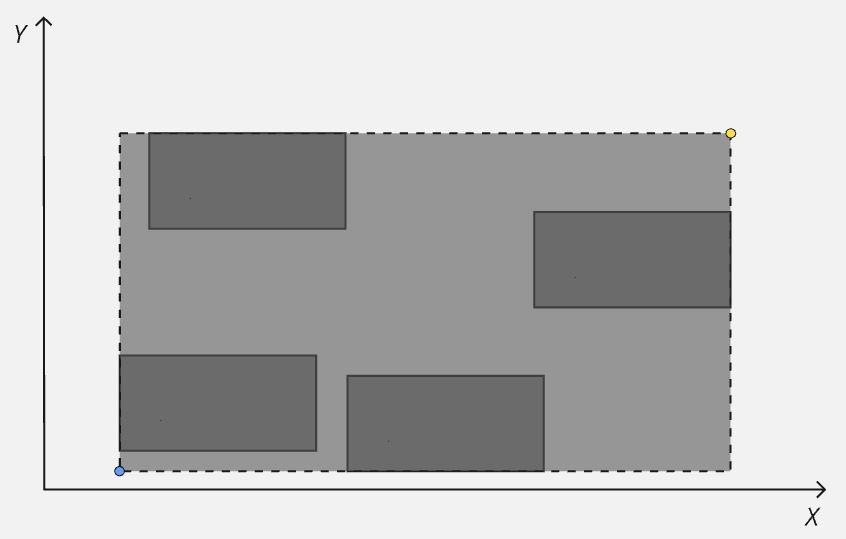
\includegraphics[width=0.6\textwidth]{figures/Orden/image.png}
  \caption{Representación gráfica del conjunto dominio de un mapa con 4 multi-intervalos, más el marcado del mínimo y máximo perimetral en azul y amarillo respectivamente.}
  \label{fig:minmaxPer1}
\end{figure}


Con toda esta información ya se puede declarar formalmente cómo está constituida la variable \texttt{pieces\_} para los \textit{piecewise maps} ordenados, denominados como \texttt{OrdPWMap}:

\begin{itemize}
  \item \texttt{pieces\_} (de tipo \textbf{OrdMapCollection}): 
  representa la colección ordenada de mapas junto con la información perimetral 
  de sus dominios.  
  En este contexto:
  \begin{itemize}
    \item \texttt{OrdMapCollection} es sinónimo de \texttt{vector<MapEntry>}.
    \item \texttt{MapEntry}, cuyas instancias denominaremos en adelante \textit{entradas de mapa}, es sinónimo de \texttt{pair<Map, SetPerimeter>}.
    \item \texttt{SetPerimeter}, cuyas instancias denominaremos en adelante \textit{perímetros}, es sinónimo de \texttt{pair<MD\_NAT, MD\_NAT>}.
  \end{itemize}
\end{itemize}


Y por último se presenta el siguiente ejemplo. Sean se los siguientes conjuntos dominio de los mapas $m_1$, $m_2$, y $m_3$ respectivamente:

\begin{itemize}
    \item $c_1 = \{[10:1:15]\times[10:1:11],[16:1:20]\times[15:1:20]\}$, con mínimo perimetral $(10,10)$
    \item $c_2 = \{[15:1:20]\times[15:1:25],[21:1:25]\times[15:1:20]\}$, con mínimo perimetral $(15,15)$
    \item $c_3 = \{[30:1:35]\times[15:1:20],[36:1:40]\times[10:1:11]\}$, con mínimo perimetral $(30,10)$
\end{itemize}

Aplicando el criterio de orden basado en los mínimos perimetrales, junto con el operador $<$ definido para la naturales multi-dimensionales, se obtiene el siguiente ordenamiento:

\begin{center}
\[
c_1 < c_2 < c_3
\]

ya que:

\[
(10,10) < (15, 15) < (30, 10)
\]

Por lo tanto, el conjunto ordenado resultante será:

\[
\ll (m_1,(minPer_1, maxPer1)),\ (m_2,(minPer_2, maxPer2)),\ (m_3, (minPer_3, maxPer3))\gg
\]
\end{center}

\section{\textit{Abstarct factory}}

Al igual que se hizo con los \textit{piecewise maps} desordenados,
también se definió la fábrica concreta para los \textit{Piecewise maps} ordenados, para poder aplicar el patrón \textit{Abstarct factory}. 

En particular, la fábrica concreta de los \textit{Piecewise maps} ordenados se denominó 
\texttt{PWMapAF}. Esta puede encontrarse en los archivos 
\textit{af\_pwmap}, tanto en su versión 
\textit{.cpp} como \textit{.hpp}, dentro de la carpeta \texttt{sbg} del repositorio.

\section{Criterios de optimización y ordenamiento}\label{sec:pwmap-opts}

En esta sección se describen en detalle los distintos \textbf{criterios de optimización} y \textbf{ordenamiento} utilizados en las operaciones sobre \textit{piecewise maps} ordenados. Ambos conjuntos de criterios serán aplicados con el propósito de mejorar la eficiencia general de dichas operaciones y reducir significativamente los tiempos de ejecución.

\textbf{Pseudocódigo y notación:} En esta sección, al igual que se hizo para los \textit{piecewise maps} desordenados, se emplearán subíndices para referirse a los mapas de un \textit{piecewise map} ordenado con el fin de aliviar la notación. Dado un \textit{piecewise map} ordenado $A$, el elemento ubicado en la posición $i$, lo cual corresponde a \texttt{pieces\_[i].first} en C++, se denotará como \textbf{$A_i$}, donde $i$ es un número natural que satisface $0 \leq i < \kappa(A)$, siendo $\kappa(A)$ la cantidad de mapas de $A$. Cabe destacar que, al tratarse de un \textit{piecewise map} ordenado, siempre se cumple que $A_i < A_j$ si y sólo si $i < j$, para todo par de $i$ y $j$ tal que $0  \leq i, j < \kappa(A)$. Adicionalmente se dirá que, en el caso anterior, $A_i$ está \textbf{antes} de $A_j$ en $A$, mientras $A_j$ está \textbf{después} de $A_i$.

\subsection{Operaciones estructuralmente similares}

Como se puede ver en la Sub-sección \ref{sec:pwmaps-des} existen muchas operaciones que presentan una estructura muy similar a la de la intersección entre conjuntos desordenados. Entre estas operaciones se encuentran: la \textbf{igualdad}, la \textbf{suma}, la i\textbf{gualdad de imágenes}, la \textbf{resta} y el \textbf{mínimo adyacente}.

Todas estas operaciones, junto con la intersección de conjuntos ordenados, comparten una estructura común que se puede dividir en dos partes: 
\begin{enumerate}
    \item Una\textbf{ fase de comparación}, donde cada elemento de uno de los argumentos es comparado con todos los del otro argumento.
    \item Un \textbf{núcleo de la operación}, donde se ejecuta la lógica específica de la operación sobre aquellos pares de elementos cuya comparación fue satisfactoria.
\end{enumerate}

Esta estructura puede observarse gráficamente en el pseudocódigo presentado en ~\ref{alg:operaciones-simil}.

En el caso de la intersección de conjuntos desordenados, la comparación consiste en verificar si la intersección entre dos multi-intervalos, uno de cada conjunto, es vacía, y el núcleo de la operación se encarga de guardar dicha intersección en el conjunto resultante.

En cambio, para las otras operaciones mencionadas, la comparación consiste en verificar si la intersección entre los dominios de dos mapas, uno de cada \textit{piecewise map} desordenado argumento, es no vacía. El núcleo depende de la operación específica: por ejemplo, en el caso de la suma, se calcula la suma de los mapas y se almacena el resultado en el \textit{piecewise map} desordenado de salida.


\begin{algorithm}
\caption{Estructura de las operaciones similares a la intersección de conjuntos desordenados}\label{alg:operaciones-simil}
\begin{algorithmic}[1]
\Require $A$, $B$ son conjuntos desordenados o dos \textit{piecewise maps} desordenados
\Function{operación}{$A, B$}

\State ... \Comment{Casos base y definiciones necesarias de la operación}

\ForAll{$a \in A$} \Comment{Fase de comparación de la operación.}
    \ForAll{$b \in B$}
        \State $I$ \Comment{Elemento a comparar proveniente de una o varias operaciones entre los elementos $a$ y $b$}
        \If{$\Call{isEmpty}{I}$}
            \State ...  \Comment{Núcleo de la operación.}
        \EndIf
    \EndFor
\EndFor

\State \Return ...
\EndFunction
\end{algorithmic}
\end{algorithm}

Por lo tanto, dado que las operaciones sobre \textit{piecewise maps} desordenados mencionadas anteriormente comparten esta misma estructura, y considerando todas las definiciones introducidas para los \textit{piecewise maps} ordenados, es posible adaptar los criterios de optimización desarrollados para la intersección de conjuntos ordenados a las operaciones mencionadas de  \textit{piecewise maps} ordenados.

\subsubsection{Criterios de optimización}

\begin{center}
    \fbox{
        \parbox{0.92\linewidth}{
            \centering
            \textbf{Criterio de parada} \\[1ex]
            \raggedright
            Sean $A$ y $B$ dos \textit{piecewise maps} ordenados. Supóngase que se está evaluando una de las operaciones mencionadas entre ambos, y en particular se consideran los posibles cálculos del núcleo de la operación entre mapa $A_i$ de $A$, con $0 \leq i < \kappa(A)$, y los mapas de $B$. Dado un índice $j$ tal que $0 \leq j < \kappa(B)$, vale lo siguiente:

            \vspace{0,5cm}
     
            \textbf{Si} el máximo perimetral del dominio de $A_i$ es estrictamente menor que el mínimo perimetral del dominio de $B_j$ en la primera dimensión, \textbf{entonces}:

            \begin{itemize}
                \item la intersección entre el dominio de $A_i$ y el de $B_{j'}$ resulta vacía \textbf{y} no se calcula el núcleo de la operación para $A_i$ y $B_{j'}$, $\forall j' \mid j \leq j' < |B|$;
                \item \textbf{y, entonces,} puede continuarse directamente con la fase de comparación entre $A_{i+1}$(si existe) y los mapas de $B$ para validar el calculo del núcleo de la operación.
            \end{itemize}
    
        }
    }
\end{center}



\begin{center}
    \fbox{
        \parbox{0.92\linewidth}{
            \centering
            \textbf{Criterio de eliminación} \\[1ex]
            \raggedright
            Sean $A$ y $B$ dos \textit{piecewise maps} ordenados. Supóngase que se está evaluando una de las operaciones mencionadas entre ambos, y en particular se consideran los posibles cálculos del núcleo de la operación entre mapa $A_i$ de $A$, con $0 \leq i < \kappa(A)$, y los mapas de $B$. Dado un índice $j$ tal que $0 \leq j < \kappa(B)$, vale lo siguiente:

            \vspace{0,5cm}
     
            \textbf{Si} el máximo perimetral del dominio de $(B_{j}$ es estrictamente menor que al mínimo perimetral del conjunto $A_{i}$ en la primera dimensión, \textbf{entonces}:

            \begin{itemize}
                \item la intersección entre $A_{i'}$ y $B_{j}$ resulta vacía \textbf{y} no se calcula el núcleo de la operación para $A_{i'}$ y $B_{j}$, $\forall i' \mid i \leq i' < \kappa(A)$;
                
                \item \textbf{y, entonces,} puede descartarse $B_j$ para las fases de comparación de los mapas posteriores a $A_i$ y así descartar completamente el calculo del núcleo de la operación $B_j$ con estos.
            \end{itemize}
                
    
        }
    }
\end{center}



\begin{center}
    \fbox{
        \parbox{0.9\linewidth}{
            \centering
            \textbf{Criterio de selección} \\[1ex]
            \raggedright
            Sean dos piecewise maps ordenados involucrados en alguna de las operaciones mencionadas. Se establece lo siguiente:

            \begin{center}
            \textit{
                Se define como $B$ a aquel piecewise map que contiene la menor cantidad de mapas,
                mientras que se denota como $A$ al piecewise map restante.
            }
            \end{center}
        }
    }
\end{center}


\begin{center}
    \fbox{
        \parbox{0.93\linewidth}{
            \centering
            \textbf{Criterio de solapamiento} \\[1ex]
            \raggedright
            Sean $A$ y $B$ dos \textit{piecewise maps}, $A_i$ un mapa de $A$ y $B_j$ uno de $B$, con índices tales que:
            \[
            0 \leq i < \kappa(A), \quad 0 \leq j < \kappa(B).
            \]
            Se establece entonces que, en el caso de realizar una de las operaciones entre $A$ y $B$, y querer calcular el núcleo de la operación entre $A_i$ y 
            $B_j$:

            \begin{itemize}
                \item \textbf{Si} existe solapamiento entre los conjuntos dominio de $A_i$ y $B_j$, \textbf{entonces}:
                \begin{itemize}
                    \item \textbf{Si} ambos conjuntos son \textit{densos}, la intersección entre ellos es necesariamente no vacía y se puede proceder con el calculo del núcleo de la operación.
                    \item \textbf{Si} al menos uno de ellos no es denso, la intersección \textit{puede} ser no vacía, pero no se garantiza de modo que se debe proceder de igual manera.
                \end{itemize}

                \item \textbf{Si} \textbf{no} existe solapamiento entre los conjuntos dominio de $A_i$ y $B_j$, \textbf{entonces} la intersección entre ellos es necesariamente vacía, independientemente de si son densos o no, y por ende puede obviarse el calculo del núcleo de la operación.
            \end{itemize}
        }
    }
\end{center}


En este último caso faltaría definir qué es el solapamiento entre conjuntos y cuándo un conjunto es denso para poder completar el criterio anterior:

        \begin{center}
            Sean $C$ y $D$ dos conjuntos. Entonces se dice que $C$ y $D$ se solapan o están solapados si y solo si los multi-intervalos definidos a través de sus mínimos y máximos perimetrales se solapan bajo la definición de solapamiento de multi-intervalos ya vista.
        \end{center}

        \begin{figure}[h]
    \centering
    \begin{subfigure}[b]{0.48\linewidth}
        \centering
        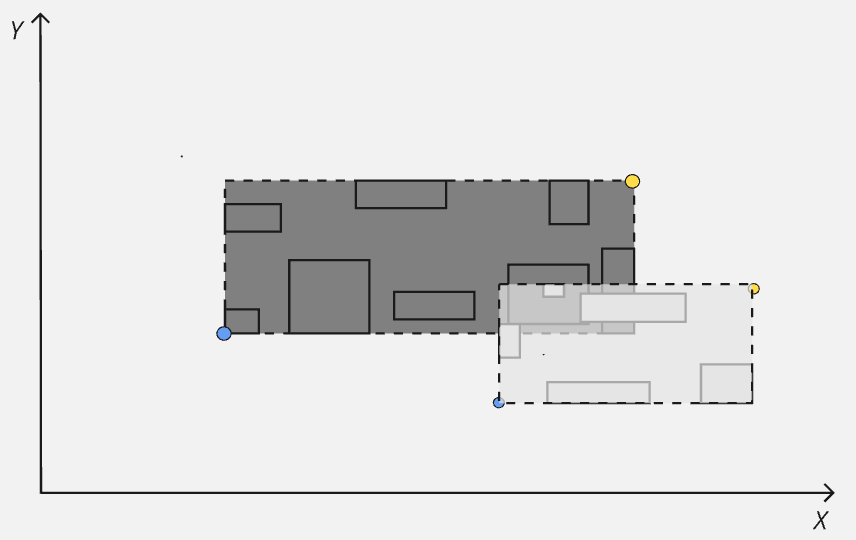
\includegraphics[width=\linewidth]{figures/optimizaciones pwmap/op simils/mi1.png}
        \caption{Conjuntos con sus multi-intervalos definidos con sus máximos y mínimos perimetrales.}
        \label{fig:crit-suma-dominio}
    \end{subfigure}
    \hfill
    \begin{subfigure}[b]{0.48\linewidth}
        \centering
        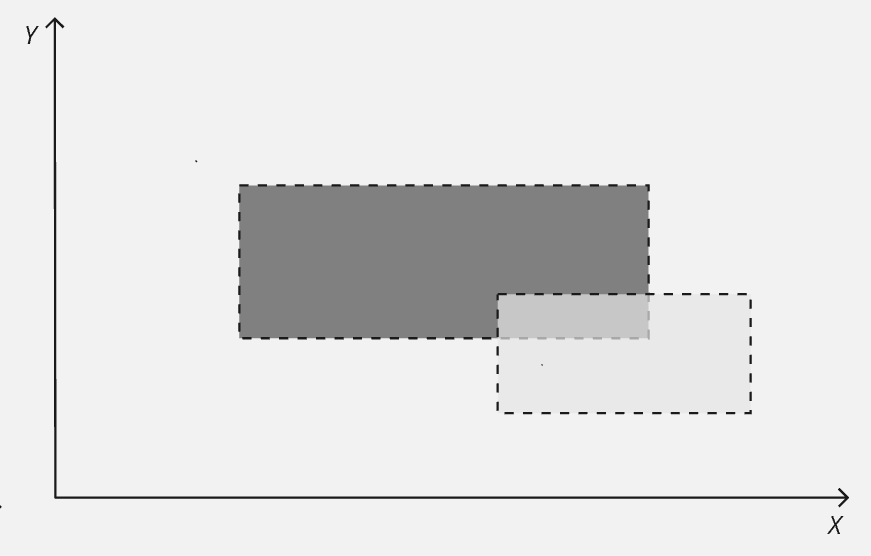
\includegraphics[width=\linewidth]{figures/optimizaciones pwmap/op simils/mi2.png}
        \caption{Solapamiento entre los multi-intervalos definidos.}
        \label{fig:crit-suma-extremos}
    \end{subfigure}
    \caption{Criterios de solapamiento para \textit{piecewise maps} ordenados.}
    \label{fig:crit-suma}
\end{figure}

        \begin{center}
            Sea $C$ el conjunto, y sean $minPer_C$ y $maxPer_C$ el mínimo y máximo perimetral, respectivamente. Entonces se dice que el conjunto es \textbf{denso} si y solo si, si se define un multi-intervalo denso $mdi$ donde su mínimo y máximo sean $minPer_C$ y $maxPer_C$ respectivamente, entonces:
                \[
                    \{mdi\} - C = C - \{mdi\} = \emptyset
                \]
        \end{center}
\begin{figure}[h]
    \centering
    \begin{subfigure}[b]{0.42\linewidth}
        \centering
        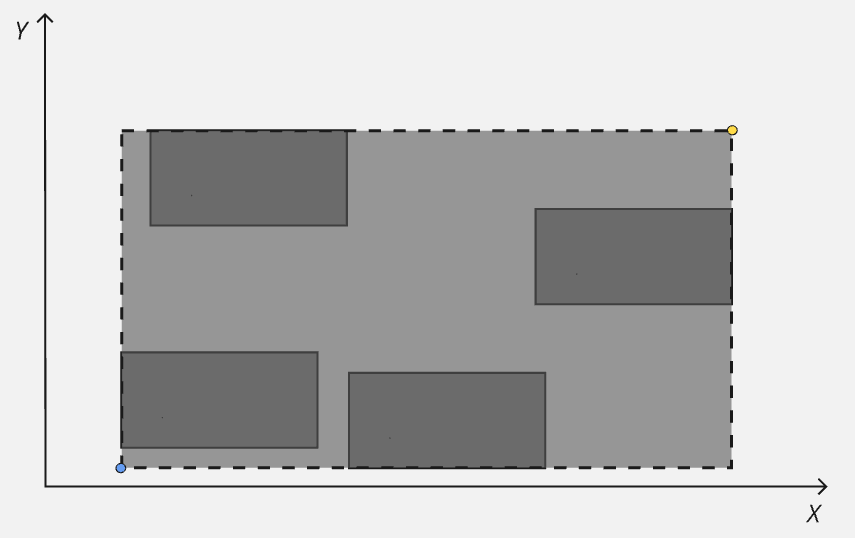
\includegraphics[width=\linewidth]{figures/optimizaciones pwmap/op simils/denso1.png}
        \caption{Conjunto no denso.}
        \label{fig:crit-suma-dominio}
    \end{subfigure}
    \hfill
    \begin{subfigure}[b]{0.42\linewidth}
        \centering
        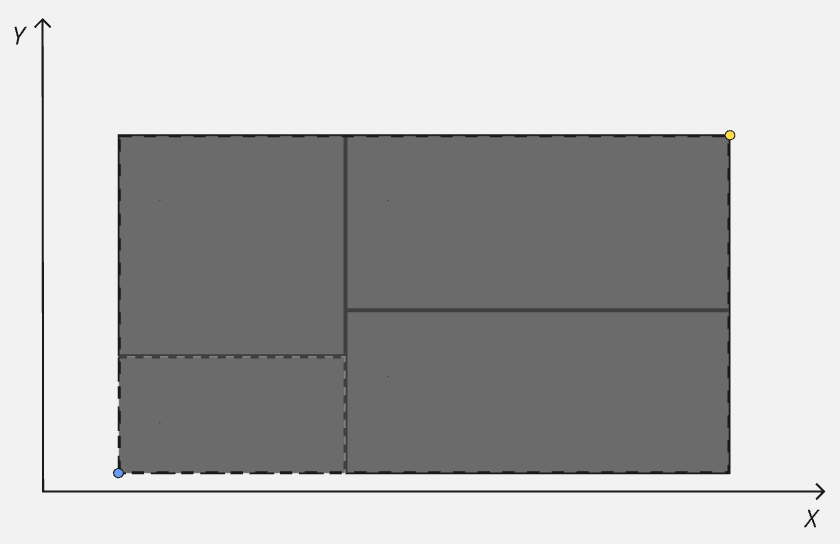
\includegraphics[width=\linewidth]{figures/optimizaciones pwmap/op simils/denso2.png}
        \caption{Conjunto no denso.}
        \label{fig:crit-suma-max}
    \end{subfigure}
    \hfill
    \vspace{0,5cm}
    \begin{subfigure}[b]{0.42\linewidth}
        \centering
        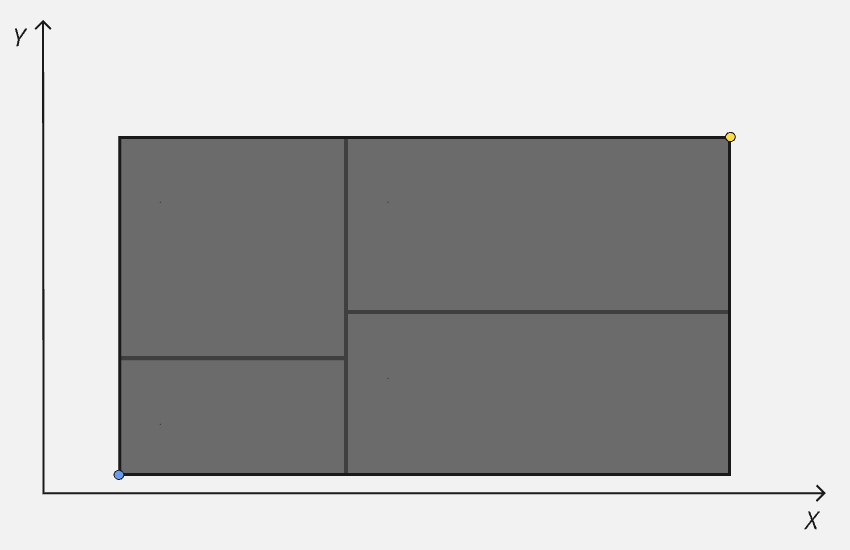
\includegraphics[width=\linewidth]{figures/optimizaciones pwmap/op simils/denso3.png}
        \caption{Conjunto denso.}
        \label{fig:crit-suma-min}
    \end{subfigure}
    \caption{Densidad de conjuntos.}
    \label{fig:crit-suma}
\end{figure}





\subsubsection{Criterios validos por operación}

Ahora bien, el núcleo de la operación puede variar significativamente dependiendo de la naturaleza de la operación considerada. En consecuencia, el criterio de ordenamiento utilizado también puede diferir considerablemente entre una operación y otra. 

Por esta razón, los criterios específicos serán mencionados y analizados individualmente, operación por operación. 

Además, no todas las operaciones admitirán todos los criterios de optimización previamente definidos. La aplicabilidad de cada criterio dependerá de las particularidades del núcleo de la operación y del comportamiento esperado.


\textbf{Igualdad - \texttt{==}}

Para el caso de la igualdad, se pueden aplicar todos los criterios de optimización previamente definidos. 

En cuanto a su \textbf{criterio de ordenamiento}, esta operación no requiere de uno, ya que no produce como resultado un \textit{piecewise map} ordenado. En consecuencia, no dispone de un criterio de ordenamiento asociado.

\textbf{suma - \texttt{+}}

En el caso de la suma, vuelven a aplicarse todos los criterios de optimización mencionados. Y, en cuanto a su criterio de ordenamiento, este resulta muy similar al propuesto para la intersección de conjuntos ordenados, con las modificaciones y adaptaciones necesarias claro esta.


\begin{center}
    \fbox{
        \parbox{0.93\linewidth}{
            \centering
            \textbf{Criterio de ordenamiento} \\[1ex]
            \raggedright
            Supóngase que se realiza la suma entre dos \textit{piecewise maps} ordenados, $A$ y $B$, y que se están evaluando las posibles sumas del $i$-ésimo mapa de $A$, denotado por $A_i$, con todos los mapas de $B$. Ademas se cuenta con un \textit{piecewise map} resultado $C$.

            \vspace{1ex}

            Todas las sumas no vacías generadas con $A_i$ deben insertarse en $C$ \textbf{después} de aquellas sumas generadas por los mapas $A_0, A_1, \dots, A_{i-1}$, cuyos mínimos perimetrales sean estrictamente menores al mínimo perimetral de $A_i$, bajo el operador $<$ de naturales multi-dimensionales.
        }
    }
\end{center}

Este criterio se basa nuevamente en la observación de que, al realizar la \textit{suma}, 
su dominio corresponde a la intersección de los dominios de los mapas participantes. 
Dicha intersección entre dos dominios está contenida en ambos, lo que implica que su mínimo perimetral 
se encuentra dentro de los multi-intervalos definidos por el mínimo y el máximo perimetral de los operandos.  

Al fijar \(A_i\), todas sus sumas posibles con mapas de \(B\) tendrán su mínimo perimetral dentro del multi-intervalo definido por el mínimo y el máximo perimetral de \(A_i\). 
Como consecuencia, cualquier suma con dominio no vacío generada tendrá un mínimo perimetral mayor o igual 
que el mínimo perimetral de \(A_i\), bajo el operador $<$ de los naturales multi-dimensionales.


Esto garantiza que tales sumas deben insertarse en el \textit{piecewise map} resultado después de aquellas cuyo 
 dominio tenga un mínimo perimetral que sea estrictamente menor,bajo el operador $<$ de los naturales multi-dimensionales, al de $A_i$, es decir, las generadas por los mapas anteriores de $A$. Una vez procesado $A_i$, se avanza hacia $A_{i+1}$ y se continúa la construcción del \textit{piecewise map} resultado de la misma manera.

La Figura~\ref{fig:crit-suma} ilustra gráficamente esta situación. Allí se observa todas las intersecciones de los dominios de las sumas producidas a partir del mapa $A_i$ con los mapas de $B$. En particular los dominios tienen el mismo nombre que los mapas a los que pertenecen. Y como se ve, estas sumas que realizan la intersección de sus dominios tienen un mínimo perimetral mayor o igual que el del dominio de $A_i$, y se insertan a continuación de los mapas previamente procesadas cuyo mínimo perimetral sea menor al de $A_i$. Esto mismo ocurre con las de $A_{i+1}$ cuya suma con $B_k$ se debe insertar después de los mapas con $A1$ y  $A2$ como dominio.

\begin{figure}[h]
    \centering
    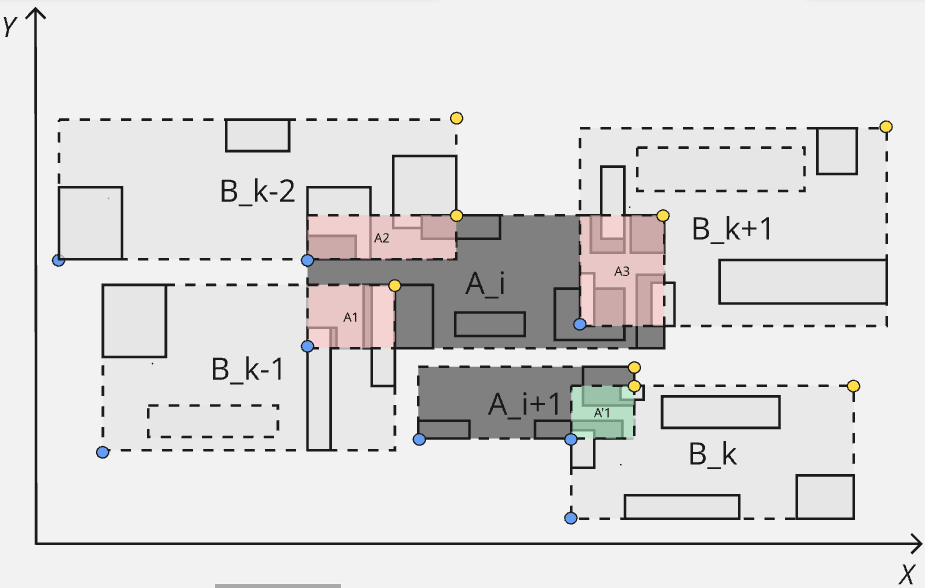
\includegraphics[width=0.8\linewidth]{figures/optimizaciones pwmap/op simils/crit suma.png}
    \caption{Criterio de ordenamiento de la suma para \textit{piecewise map} ordenados de las sumas en función de su dominio y, en particular, de sus mínimos perimetrales.}
    \label{fig:crit-suma}
\end{figure}

Adicionalmente, no es necesario comenzar a verificar la posición de inserción de las sumas en el \textit{piecewise map} resultado desde el principio en cada iteración de los elementos de $A$. Dado el orden intrínseco de los \textit{piecewise map} involucrados, se cumple que
\[
minPer_{i} \leq minPer_{i+1}
\]
 donde $minPer_i$ y $minPer_{i+1}$ son los minimos perimetrales de $A_i$ y $A_{i+1}$ respectivamente.
 
Esto implica que las sumas generadas por $A_{i+1}$ necesariamente deben insertarse a partir de una posición igual o posterior a aquella donde comenzaron a colocarse las sumas de $A_i$ con los elementos de $B$.

Esto desencadena la siguiente modificación del criterio de ordenamiento: 
\begin{center}
    \fbox{
        \parbox{0.93\linewidth}{
            \centering
            \textbf{Criterio de ordenamiento} \\[1ex]
            \raggedright
            Supóngase que se realiza la suma entre dos \textit{piecewise maps} ordenados, $A$ y $B$, y que se están evaluando las posibles sumas del $i$-ésimo mapa de $A$, denotado por $A_i$, con todos los mapas de $B$. Ademas se cuenta con un \textit{piecewise map} resultado $C$.

            \vspace{1ex}

            Todas las sumas no vacías generadas con $A_i$ deben insertarse en $C$ \textbf{después} de aquellas sumas generadas por los mapas $A_0, A_1, \dots, A_{i-1}$, cuyos mínimos perimetrales sean estrictamente menores al mínimo perimetral $A_i$, bajo el operador $<$ de naturales multi-dimensionales.
            
            \vspace{1ex}

            Adicionalmente \textbf{si} la posición a partir de la cual se colocan las sumas de $A_i$ en el \textit{piecewise map} resultante es $j$, con $0 \leq j < \kappa(C)$, \textbf{entonces} aquellas generadas por $A_{i+1}$ se insertaran a partir de $j'$ tal que $j \leq j' < \kappa(C)$.
        }
    }
\end{center}

\textbf{Igualdad de imágenes - \texttt{equalImage}}

El caso de esta operación es muy similar al de la operación de igualdad: admite todos los criterios de optimización y tampoco requiere un criterio de ordenamiento. Esta última característica, a diferencia del caso de la igualdad, no se debe a que la operación devuelva un valor de verdad, sino a que su resultado es un conjunto en sí mismo, el cual tiene su implementación propia y no se debe alterar.


\textbf{Mínimo adyacente - \texttt{minAdjMap}}

Ahora es el turno de la operación \texttt{minAdjMap}, la cual puede utilizar todos los criterios de optimización, salvo el de selección, ya que nuevamente el orden de los argumentos tiene relevancia. 

En cuanto al criterio de ordenamiento, aparece un problema que se repite tanto aquí como en varias operaciones sobre \textit{piecewise maps} ordenados: la imagen. La imagen de un mapa, aunque es un conjunto, posee una cohesión que depende tanto del conjunto dominio como de la colección de expresiones lineales del mapa. Por ejemplo, dos mapas pueden tener un mismo dominio, pero basta con que alguna de sus expresiones varíe para que sus imágenes sean distintas. Algo similar ocurre si varía el dominio.

Entonces, ordenar mapas cuyo dominio corresponde a la imagen resulta una tarea particularmente compleja. En estos casos, el orden del \textit{piecewise map} original aporta escasa o nula información útil para ordenar los mapas derivados, cuyos dominios provienen de una imagen. 

Una alternativa es realizar un ordenamiento estrictamente lineal, lo cual implica un costo computacional elevado, especialmente cuando el \textit{piecewise map} resultante contiene un gran número de mapas.


En conclusión, para poder brindar un orden a un \textit{piecewise map} cuyo contenido son mapas con dominios derivados de imágenes, sería necesario tener en cuenta no solo el dominio, sino también las expresiones y la forma de dichas expresiones. Por esta razón, se concluyó que lo más óptimo es utilizar un algoritmo de ordenamiento preexistente, lo cual simplifica el entendimiento de esta y de las demás operaciones de \textit{piecewise maps} ordenados. Así se evita la necesidad de escribir y mantener código de criterios de ordenamiento que, probablemente, tendría un rendimiento inferior.


\textbf{Resta - \texttt{-}}

Por ultimo se encuentra la operación \texttt{-}, la cual admite todos los criterios de optimización, con excepción del criterio de selección, ya que se trata de una operación donde el orden de los argumentos es relevante y, por lo tanto, no puede alterarse. En cuanto al orden de la salida, ocurre algo particular. 

En el núcleo de la operación desordenada, cuando se calcula la resta entre dos mapas, el proceso genera un resultado parcial únicamente para los dos mapas involucrados. El tamaño de este resultado parcial, o la cantidad de mapas que contiene, depende exclusivamente de la cantidad de dimensiones con las que se esté trabajando. Luego, este resultado parcial se incorpora al \textit{piecewise map} resultado de la operación.

Ahora bien, para garantizar que la salida se encuentre correctamente ordenada, se optó por emplear un algoritmo de ordenamiento preexistente. De este modo, se evita mantener la invariante de orden durante la operación en el \textit{piecewise map} resultante y en el resultado parcial, y en su lugar, antes de devolver el \textit{piecewise map} resultante, se procede a ordenarlo utilizando dicho algoritmo.

De esta forma, se evita recurrir a estrategias ineficientes, como ordenar cada resultado parcial para luego aplicar la operación \texttt{concatenation}.

\subsection{Restricción de dominio - \texttt{restrict}}

El caso de la operación \texttt{restrict} es diferente al de las operaciones vistas anteriormente. Sin embargo, esto no significa que no puedan adaptarse los criterios definidos previamente para esta operación.

En particular, la operación \texttt{restrict} aplicada a un \textit{piecewise map} desordenado, como ya se vio, consiste en restringir el dominio de cada uno de sus mapas individuales en base a un conjunto, siendo ambos argumentos de la operación, y quedando como parte del resultado solo aquellos mapas del \textit{piecewise map} desordenado cuyos dominios restringidos son no vacíos.

Ahora bien, al dotar de orden al \textit{piecewise map} argumento y requerir que el resultado también esté ordenado, la operación puede beneficiarse de los siguientes criterios de optimización y ordenamiento:

\subsubsection{Criterios de optimización}


\begin{center}
    \fbox{
        \parbox{0.92\linewidth}{
            \centering
            \textbf{Criterio de parada} \\[1ex]
            \raggedright
            Sean $A$ un \textit{piecewise map} ordenado y $S$ un conjunto. Supóngase que se evalúa la restricción de dominio entre ambos, y en particular se considera la posible restricción de domino del dominio de un mapa $A_i$ de $A$, con $0 \leq i < \kappa(A)$, con respecto a $S$. Entonces vale lo siguiente:

            \vspace{0,5cm}
     
            \textbf{Si} el máximo perimetral de $S$ es estrictamente menor que el mínimo perimetral del conjunto dominio de $A_i$ en la primera dimensión, \textbf{entonces}:

            \begin{itemize}
                \item la intersección entre el dominio de $A_i$ y $S$ resulta vacía \textbf{y} no se calcula la restricción de dominio para $A_{i'}$ con respecto a $S$, $\forall i' \mid i \leq i' < \kappa(A)$;
                \item \textbf{y, entonces,} puede terminarse directamente con la operación \texttt{restrict}.
            \end{itemize}
    
        }
    }
\end{center}


\begin{center}
    \fbox{
        \parbox{0.93\linewidth}{
            \centering
            \textbf{Criterio de solapamiento} \\[1ex]
            \raggedright
            Sean $A$ un \textit{piecewise map}, $S$ un conjunto y $A_i$ un mapa de $A$ tal que:
            \[
            0 \leq i < \kappa(A).
            \]
            Se establece entonces que, en el caso de realizar la restricción de dominio de $A$ sobre $S$ y querer calcular la restricción de $A_i$ con respecto a $S$:

            \begin{itemize}
                \item \textbf{Si} existe solapamiento entre el conjunto dominio de $A_i$ y $S$, \textbf{entonces}:
                \begin{itemize}
                    \item \textbf{Si} ambos conjuntos son \textit{densos}, la intersección entre ellos es necesariamente no vacía y se puede proceder con el calculo de la restricción del dominio de $A_i$ en base a $S$.
                    \item \textbf{Si} al menos uno de ellos no es denso, la intersección \textit{puede} ser no vacía, pero no se garantiza de modo que se debe proceder de igual manera.
                \end{itemize}

                \item \textbf{Si} \textbf{no} existe solapamiento entre el conjunto dominio de $A_i$ y $S$, \textbf{entonces} la intersección entre ellos es necesariamente vacía, independientemente de si son densos o no, y por ende puede obviarse el calculo de la restricción del dominio de $A_i$ en base a $S$.
            \end{itemize}
        }
    }
\end{center}

\subsubsection{Criterio de ordenamiento}

En este caso, lo que debe mantenerse ordenado en el \textit{piecewise map} resultante son todas las restricciones de dominio no vacías de los mapas del \textit{piecewise map} ordenado argumento. La restricción de dominio de un mapa consiste únicamente en reemplazar su dominio original por la intersección entre dicho dominio y el conjunto que también llega como argumento.

Ahora bien, como se discutió en el criterio de ordenamiento para la suma, el mínimo perimetral del dominio restringido está contenido dentro de alguno de los multi-intervalos definidos por los máximos y mínimos perimetrales del dominio del mapa a restringir y del conjunto que restringe. Ademas aquí también vale que no es necesario buscar la posición de inserción desde el comienzo del \textit{piecewise map} resultado. Esto permite redefinir el criterio de ordenamiento de la siguiente manera:

\begin{center}
    \fbox{
        \parbox{0.93\linewidth}{
            \centering
            \textbf{Criterio de ordenamiento} \\[1ex]
            \raggedright
            Supóngase que se realiza la restricon de dominio entre un \textit{piecewise map} ordenado $A$ y un conjunto $S$, y que se están evaluando la restricción de dominio del $i$-ésimo mapa de $A$, denotado por $A_i$, con respecto a $S$. Ademas se cuenta con un \textit{piecewise map} resultado $C$.

            \vspace{1ex}

            La restricción no vacía generada con $A_i$ deben insertarse en $C$ \textbf{después} de aquellas restricciones no vacías generadas por los mapas $A_0, A_1, \dots, A_{i-1}$, cuyos mínimos perimetrales sean estrictamente menores al mínimo perimetral de $A_i$, bajo el operador $<$ de naturales multi-dimensionales.

            \vspace{1ex}

            Adicionalmente \textbf{si} la posición a partir de la cual se colocan las sumas de $A_i$ en el \textit{piecewise map} resultante es $j$, con $0 \leq j < \kappa(C)$, \textbf{entonces} aquellas generadas por $A_{i+1}$ se insertaran a partir de $j'$ tal que $j \leq j' < \kappa(C)$.
        }
    }
\end{center}


\subsection{Combinación - \texttt{combine}}

El siguiente caso que se analizará es el de la operación \texttt{combine}, una de las ya introducidas previamente en el capítulo de conceptos preliminares.

Esta operación, como ya se vio, aplicada sobre \textit{piecewise maps} desordenados, toma dos de ellos y realiza una suerte de unión, devolviendo un único \textit{piecewise map} desordenado. Este contiene todos los mapas del primero, junto con aquellos mapas del segundo cuyos dominios son una restricción, conteniendo ahora solo aquellos valores no presentes en el dominio total del primer \textit{piecewise map}. 

Debido a la naturaleza de su funcionamiento y requerir preservar el orden en el resultado, esta operación emplea únicamente un criterio de optimización y un criterio de ordenamiento, ambos reformulados de los vistos para las \textit{operaciones estructuralmente similares}.

\subsubsection{Criterio de optimización}

Trabajando con dos \textit{piecewise maps} $A$ y $B$, los únicos mapas de $B$ que pueden formar parte del resultado son aquellos donde la diferencia de su domino con el dominio total de $A$ sea no vacía. El dominio modificado resultante para cada uno de los mapas de $B$ será precisamente dicha diferencia. Por lo tanto, lo único que se puede hacer es omitir la diferencia cuando se sabe que no es necesaria, y de esta observación se deriva el siguiente criterio de solapamiento:

\begin{center}
    \fbox{
        \parbox{0.93\linewidth}{
            \centering
            \textbf{Criterio de solapamiento} \\[1ex]
            \raggedright
            Sean $A$ y $B$ dos \textit{piecewise maps}, $B_j$ un mapa de $B$, tal que:
            \[
            0 \leq j < \kappa(B).
            \]
            y sea $S$ el dominio de $A$. Se establece entonces que, en el caso de realizar la combinación entre $A$ y $B$ y al estar considerando $B_j$ :

            \begin{itemize}
                \item \textbf{Si} existe solapamiento entre el conjunto dominio de $B_j$ y $S$, \textbf{entonces}:
                \begin{itemize}
                    \item \textbf{Si} ambos conjuntos son \textit{densos}, la intersección entre ellos es necesariamente no vacía y se debe proceder con el calculo de la diferencia para obtener el nuevo dominio de $B_j$.
                    \item \textbf{Si} al menos uno de ellos no es denso, la intersección \textit{puede} ser no vacía, pero no se garantiza de modo que se debe proceder de igual manera.
                \end{itemize}

                \item \textbf{Si} \textbf{no} existe solapamiento entre el conjunto dominio de $B_j$ y $S$, \textbf{entonces} la intersección entre ellos es necesariamente vacía, independientemente de si son densos o no, y por ende puede obviarse el calculo de la diferencia,la cual devolvería el mismo dominio de $B_j$, y el dominio de $B_k$ queda intacto.
            \end{itemize}
        }
    }
\end{center}

\subsubsection{Criterio de ordenamiento}

En cuanto al orden, al realizar la diferencia entre dos conjuntos, por ejemplo, entre dos conjuntos $C$ y $D$, el nuevo mínimo perimetral del conjunto resultante $C - D$ debe encontrarse contenido dentro del multi-intervalo definido por el mínimo y el máximo perimetral del conjunto original $C$. 

Esto se debe a que la operación de diferencia remueve elementos de $C$, sin añadir otros nuevos. Esta observación es casi análoga a lo que ocurría en el caso de la operación de suma, discutido en en este capitulo con respecto a la suma de \textit{piecewise map} ordenados. Análogamente a lo visto también en la suma, gracias a lo anterior y al orden de los \textit{piecewise maps}, ocurre que si $B_j$ con su dominio modificado se debería insertar a partir de una posición $i$, con $0 \leq i < \kappa(C)$, en el \textit{piecewise map} resultado, entonces $B_j$ con su dominio modificado debería ubicarse en $i'$ tal que $i \leq i' < \kappa(C)$

En consecuencia, se postula el siguiente criterio de ordenamiento derivado del visto para el operador \texttt{+}:

\begin{center}
    \fbox{
        \parbox{0.93\linewidth}{
            \centering
            \textbf{Criterio de ordenamiento} \\[1ex]
            \raggedright
            Supóngase que se realiza la combinación entre dos \textit{piecewise maps} ordenados, $A$ y $B$, y que se deba calcular el nuevo dominio para el mapa $j$-ésimo de $B$, denotado por $B_j$, con respecto al dominio de $A$, $S$. Ademas se cuenta con un \textit{piecewise map} resultado $C$.

            \vspace{1ex}

            \textbf{Si} el nuevo dominio de $B_j$ no es vacío, es decir, la resta entre el conjunto dominio de $B_j$ y $S$ es no vacía; \textbf{entonces} el mapa $B_j$ con dominio restringido por $S$ estará ubicado en el \textit{piecewise map} resultante después de todos aquellos mapas cuyo mínimo perimetral sea menor que el minino perimetral del dominio original de $B_j$, bajo el operador $<$ de naturales multi-dimensionales.
            
            \vspace{1ex}

            Adicionalmente \textbf{si} la posición a partir de la cual se coloca de $B_j$ con dominio modificado en el \textit{piecewise map} resultante es $i$, con $0 \leq i < \kappa(C)$, \textbf{entonces} el mapa modificado de $B_{j+1}$ se insertaría, si su dominio no es vacío, a partir de $i'$ tal que $i \leq i' < \kappa(C)$.
        }
    }
\end{center}


\subsection{Concatenación - \texttt{concatenation}}

El caso de la operación concatenación, es básicamente homólogo al del la unión disjunta de conjuntos, y por ende haciendo las respectivas modificaciones, se puede reutilizar lo visto para la unión disjunta de conjuntos ordenados aquí.

\subsubsection{Criterio de ordenamiento}

\begin{center}
    \fbox{
        \parbox{0.93\linewidth}{
            \centering
            \textbf{Criterio de ordenamiento}\\[1ex]
            \raggedright
           Sean $A = \{A_0, A_1, \dots, A_{n-1}\}$ y $B = \{B_0, B_1, \dots, B_{m-1}\}$ dos \textit{piecewise maps} no vacíos, disjuntos y ordenados. Sea $C$ un \textit{piecewise map} inicialmente vacío que contendrá el resultado de la fusión ordenada de $A$ y $B$. Y sean $A_i$ un mapa de $A$ y $B_j$ un mapa de $B$, con índices tales que:
            \[
            0 \leq i < \kappa(A), \quad 0 \leq j < \kappa(B).
            \]
            
            \vspace{1ex}

            Entonces, al realizar la unión disjunta entre $A$ y $B$ vale que:

            \begin{itemize}
                \item \textbf{Si} el mínimo perimetral de  $A_i$ es menor, bajo el operador $<$ definido para naturales multi-dimensionales, que el mínimo perimetral de  $B_j$, entonces $A_i$ debe aparecer \textbf{antes} que $B_j$ en el \textit{piecewise map} $C$.
                \item\textbf{Si} el mínimo perimetral de  $A_i$ no es menor, bajo el operador $<$ definido para naturales multi-dimensionales, que el mínimo perimetral de $B_j$, entonces $B_j$ debe aparecer \textbf{antes} que $A_i$ en el \textit{piecewise map} $C$.
            \end{itemize}

            \vspace{1ex}
        }
    }
\end{center}

\subsection{Desplazamiento de dominio - \texttt{offsetDom}}

Al buscar optimizar y ordenar la salida en la operación \texttt{offsetDom}, cuando esta recibe como argumentos dos \textit{piecewise maps} ordenados, es posible adaptar y reutilizar los criterios previamente establecidos para la operación \texttt{restrict}.

Como se observa en su versión desordenada, para que un mapa de $A$ sea incluido en el resultado, debe existir un desplazamiento no vacío generado por la imagen de $O$ en base al dominio del mapa. Ahora bien, al trabajar con \textit{piecewise maps} ordenados, es posible anticipar si dicho desplazamiento será vacío o no. Para ello, pueden aplicarse criterios de optimización derivados, y adaptados, de aquellos utilizados en la restricción de dominio.

Cabe destacar que, al trabajar con la imagen de un \textit{piecewise map} para generar la salida, 
nuevamente se hará uso de un algoritmo de ordenamiento en lugar de diseñar un criterio de ordenamiento específico, como se hizo para \textit{minAdjMap}.


\subsubsection{Criterios de optimización}


\begin{center}
    \fbox{
        \parbox{0.92\linewidth}{
            \centering
            \textbf{Criterio de parada} \\[1ex]
            \raggedright
            Sean $A$ y $O$ \textit{piecewise maps} ordenados y $S$ el conjunto dominio de $O$. Supóngase que se evalúa el desplazamiento de dominio entre $A$ y $O$, y en particular se considera el posible desplazamiento de dominio del dominio de un mapa $A_i$ de $A$, con $0 \leq i < \kappa(A)$, con respecto a $O$. Entonces vale lo siguiente:

            \vspace{0,5cm}
     
            \textbf{Si} el máximo perimetral de $S$ es estrictamente menor que el mínimo perimetral del conjunto dominio de $A_i$ en la primera dimensión, \textbf{entonces}:

            \begin{itemize}
                \item la intersección entre el dominio de $A_i$ y $S$ resulta vacía \textbf{y} no se calcula el desplazamiento de dominio para $A_{i'}$ con respecto a $S$, $\forall i' \mid i \leq i' < \kappa(A)$;
                \item \textbf{y, entonces,} puede terminarse directamente con la operación \texttt{offsetDom}.
            \end{itemize}
    
        }
    }
\end{center}


\begin{center}
    \fbox{
        \parbox{0.93\linewidth}{
            \centering
            \textbf{Criterio de solapamiento} \\[1ex]
            \raggedright
            Sean $A$ y $O$ \textit{piecewise maps} ordenados, $S$ el conjunto dominio de $O$ y $A_i$ un mapa de $A$ tal que:
            \[
            0 \leq i < \kappa(A).
            \]
            Se establece entonces que, en el caso de realizar el desplazamiento de dominio de $A$ en base a $O$, y querer desplazar el dominio de $A_i$ en base a $O$:

            \begin{itemize}
                \item \textbf{Si} existe solapamiento entre el conjunto dominio de $A_i$ y $S$, \textbf{entonces}:
                \begin{itemize}
                    \item \textbf{Si} ambos conjuntos son \textit{densos}, la intersección entre ellos es necesariamente no vacía y se puede proceder con el calculo del desplazamiento de dominio de $A_i$ en base a $O$.
                    \item \textbf{Si} al menos uno de ellos no es denso, la intersección \textit{puede} ser no vacía, pero no se garantiza de modo que se debe proceder de igual manera.
                \end{itemize}

                \item \textbf{Si} \textbf{no} existe solapamiento entre el conjunto dominio de $A_i$ y $S$, \textbf{entonces} la intersección entre ellos es necesariamente vacía, independientemente de si son densos o no, y por ende puede obviarse el calculo del desplazamiento de dominio de $A_i$ en base a $O$.
            \end{itemize}
        }
    }
\end{center}


\subsection{Composición - \texttt{composition}}

Al intentar optimizar y ordenar el \textit{piecewise map} resultante en la operación \texttt{composition}, cuando esta recibe como argumentos dos \textit{piecewise maps} ordenados, es posible adaptar y reutilizar los criterios previamente establecidos para la operación suma y para las \textit{operaciones estructuralmente similares}.

Como se observa en su versión desordenada optimizada ~\ref{alg:composition-des-opt}, para que el resultado de componer un mapa de $A$, $a$, con uno de $B$, $b$, sea incluido en el resultado final, debe tener un dominio no vacío. Es decir, la intersección del domino $a$ con la imagen de $b$ debe ser no vacía. Teniendo esto último presente se pueden redefinir los criterios de optimización para las \textit{operaciones estructuralmente similares} y el criterio de ordenamiento que se le dio a la suma. 

\subsubsection{Criterios de optimización}


\begin{center}
    \fbox{
        \parbox{0.92\linewidth}{
            \centering
            \textbf{Criterio de parada} \\[1ex]
            \raggedright
            Sean $A$ y $B$ dos \textit{piecewise maps} ordenados. Supóngase que se está evaluando la composición entre ambos, y en particular se consideran las posibles composiciones entre un mapa $B_j$ de $B$, con $0 \leq j < \kappa(B)$, y los mapas de $A$. Dado un índice $i$ tal que $0 \leq i < \kappa(A)$, vale lo siguiente:

            \vspace{0,5cm}
     
            \textbf{Si} el máximo perimetral del dominio de $A_i$ es estrictamente menor que el mínimo perimetral del conjunto imagen de $B_j$ en la primera dimensión, \textbf{entonces}:

            \begin{itemize}
                \item la intersección entre el dominio de $A_{i'}$ y la imagen de $B_{j}$ resulta vacía \textbf{y} no se calcula la composición entre $A_{i'}$ y $B_{j}$, $\forall i' \mid i \leq i' < \kappa(A)$;
                \item \textbf{y, entonces,} puede continuarse directamente con verificando las posibles composiciones de $B_{j+1}$(si existe) con los mapas de $A$.
            \end{itemize}
    
        }
    }
\end{center}

\begin{center}
    \fbox{
        \parbox{0.93\linewidth}{
            \centering
            \textbf{Criterio de solapamiento} \\[1ex]
            \raggedright
            Sean $A$ y $B$ dos \textit{piecewise maps}, $A_i$ un mapa de $A$ y $B_j$ uno de $B$, con índices tales que:
            \[
            0 \leq i < \kappa(A), \quad 0 \leq j < \kappa(b).
            \]
            Se establece entonces que, en el caso de realizar la composición entre $A$ y $B$, y querer calcular la composición de $A_i$ y $B_j$:

            \begin{itemize}
                \item \textbf{Si} existe solapamiento entre los conjuntos dominio de $A_i$ e imagen de $B_j$, \textbf{entonces}:
                \begin{itemize}
                    \item \textbf{Si} ambos conjuntos son \textit{densos}, la intersección entre ellos es necesariamente no vacía y se puede proceder con el calculo de la composición entre $A_i$ y $B_j$.
                    \item \textbf{Si} al menos uno de ellos no es denso, la intersección \textit{puede} ser no vacía, pero no se garantiza de modo que se debe proceder de igual manera.
                \end{itemize}

                \item \textbf{Si} \textbf{no} existe solapamiento entre los conjuntos dominio de $A_i$ e imagen de $B_j$, \textbf{entonces} la intersección entre ellos es necesariamente vacía, independientemente de si son densos o no, y por ende puede obviarse el calculo de la composición entre $A_i$ y $B_j$.
            \end{itemize}
        }
    }
\end{center}

\subsubsection{Criterio de ordenamiento}

En este caso tenemos que al realizar la composición entre dos mapas, su dominio es un subconjunto del dominio original del primer mapa a componer. Por ende, al fijar el primer mapa, todos sus composiciones no vacías con otros mapas, tendrán un domino con un mínimo perimetral igual o menor que el del dominio del mapa fijado, bajo el operador $<$ de naturales multi-dimensionales. Esto es muy similar a lo que ocurría en la operación \textit{restrict}. Ademas aquí también vale que no es necesario buscar la posición de inserción desde el comienzo del \textit{piecewise map} resultado como se vio para las restricción de dominio.

  
\begin{center}
    \fbox{
        \parbox{0.93\linewidth}{
            \centering
            \textbf{Criterio de ordenamiento} \\[1ex]
            \raggedright
            Supóngase que se realiza la composición entre dos \textit{piecewise maps} ordenados, $A$ y $B$, y que se están evaluando las posibles composiciones del $j$-ésimo mapa de $B$, denotado por $B_j$, con todos los mapas de $A$. Ademas se cuenta con un \textit{piecewise map} resultado $C$.

            \vspace{1ex}

            Todas las composiciones no vacías generadas con $B_j$ deben insertarse en $C$ \textbf{después} de aquellas composiciones generadas por los mapas $B_0, B_1, \dots, B_{k-1}$, cuyos mínimos perimetrales sean estrictamente menores al mínimo perimetral de $B_j$, bajo el operador $<$ de naturales multi-dimensionales.

            \vspace{1ex}

            Adicionalmente \textbf{si} la posición a partir de la cual se colocan las composiciones de $B_j$ en el \textit{piecewise map} resultante es $i$, con $0 \leq i < |C|$, \textbf{entonces} aquellas generadas por $B_{j+1}$ se insertaran a partir de $i'$ tal que $i \leq i' < \kappa(C)$.
        }
    }
\end{center}


\subsection{Pseudoinversa - \texttt{firstInv}}

El caso de la operación \texttt{firstInv} resulta particularmente interesante, ya que permite aplicar criterios de optimización tanto entre los elementos de la entrada, como en elementos del propio algoritmo interno de la misma operación.

Tal como se observa en su versión desordenada y optimizada, para que un mapa $A$ sea considerado para el cálculo interno de la operación, la diferencia entre la imagen del mapa restringida al subdominio $S$ y el conjunto de elementos ya visitados, denotado como $visited$, debe ser no vacía. Esto puede suceder si, y solo si, se cumplen simultáneamente las siguientes condiciones:
\begin{itemize}
    \item La imagen de $A$ restringida al subdominio $S$ es no vacía.
    \item La diferencia entre dicha imagen y el conjunto $visited$ es también no vacía.
\end{itemize}

Esto permite aplicar entonces dos conjuntos de criterios de optimización: uno entre los mapas del \textit{piecewise map} y el conjunto que llegan como argumento y otro entre los mapas del \textit{piecewise map} y el conjunto de valores visitados $visited$.

Dado que aquí también se trabaja sobre la imagen en la generación de la salida, el ordenamiento de la misma queda delegado a un algoritmo de ordenamiento preexistente nuevamente. No obstante, los criterios de optimización aplicables serán presentados a continuación.

\subsubsection{Criterios de optimización}


\begin{center}
    \fbox{
        \parbox{0.92\linewidth}{
            \centering
            \textbf{Criterio de parada} \\[1ex]
            \raggedright
            Sean $A$ un \textit{piecewise map} ordenado y $S$ un conjunto. Supóngase que se evalúa la pseudoinversa entre ambos, y en particular se considera la posible pseudoinversión de un mapa $A_i$ de $A$, con $0 \leq i < \kappa(A)$, con respecto a $S$. Entonces vale lo siguiente:

            \vspace{0,5cm}
     
            \textbf{Si} el máximo perimetral de $S$ es estrictamente menor que el mínimo perimetral del conjunto dominio de $A_i$ en la primera dimensión, \textbf{entonces}:

            \begin{itemize}
                \item la intersección entre el dominio de $A_i$ y $S$ resulta vacía \textbf{y} no se calcula la pseudoinversión de $A_{i'}$ con respecto a $S$, $\forall i' \mid i \leq i' < \kappa(A)$;
                \item \textbf{y, entonces,} puede terminarse directamente con la operación \texttt{firstInv}.
            \end{itemize}
    
        }
    }
\end{center}


\begin{center}
    \fbox{
        \parbox{0.93\linewidth}{
            \centering
            \textbf{Criterio de solapamiento} \\[1ex]
            \raggedright
            Sean $A$ un \textit{piecewise map}, $S$ un conjunto y $A_i$ un mapa de $A$ tal que:
            \[
            0 \leq i < \kappa(A).
            \]
            Se establece entonces que, en el caso de realizar la pseudoinversa de $A$ en base a $S$ y querer calcular la pseudoinversión de $A_i$ con respecto a $S$:

            \begin{itemize}
                \item \textbf{Si} existe solapamiento entre el conjunto dominio de $A_i$ y $S$, \textbf{entonces}:
                \begin{itemize}
                    \item \textbf{Si} ambos conjuntos son \textit{densos}, la intersección entre ellos es necesariamente no vacía y se puede proceder con el calculo de la imagen de $A_i$ en base a $S$ para el calculo de la pseudoinversión de $A_i$ en base a $S$.
                    \item \textbf{Si} al menos uno de ellos no es denso, la intersección \textit{puede} ser no vacía, pero no se garantiza de modo que se debe proceder de igual manera.
                \end{itemize}

                \item \textbf{Si} \textbf{no} existe solapamiento entre el conjunto dominio de $A_i$ y $S$, \textbf{entonces} la intersección entre ellos es necesariamente vacía, independientemente de si son densos o no, y por ende puede obviar el calculo de la imagen de $A_i$ en base a $S$ y el calculo de la pseudoinversión de $A_i$ en base a $S$.
            \end{itemize}
        }
    }
\end{center}

\begin{center}
    \fbox{
        \parbox{0.93\linewidth}{
            \centering
            \textbf{Criterio de solapamiento para $visited$} \\[1ex]
            \raggedright
            Sean $A$ un \textit{piecewise map}, $S$ un conjunto y $A_i$ un mapa de $A$ tal que:
            \[
            0 \leq i < \kappa(A),
            \]
            sea $I$ la imagen no vacia de $A_i$ en base a $S$ y $visited$ el conjunto de valores ya visitados por las pseudoinversas de los mapas anteriores a $A_i$.
            Se establece entonces que, en el caso de realizar la pseudoinversa de $A$ en base a $S$ y querer calcular la pseudoinversión de $A_i$ con respecto a $S$:

            \begin{itemize}
                \item \textbf{Si} existe solapamiento entre el conjunto $I$ y $visited$, \textbf{entonces}:
                \begin{itemize}
                    \item \textbf{Si} ambos conjuntos son \textit{densos}, la intersección entre ellos es necesariamente no vacía y se puede proceder con el calculo de la pseudoinversión de $A_i$ en base a $S$ y utilizando $I-visited$ de no ser vacía.
                    \item \textbf{Si} al menos uno de ellos no es denso, la intersección \textit{puede} ser no vacía, pero no se garantiza de modo que se debe proceder de igual manera.
                \end{itemize}

                \item \textbf{Si} \textbf{no} existe solapamiento entre el conjunto dominio de $A_i$ y $S$, \textbf{entonces} la intersección entre ellos es necesariamente vacía, independientemente de si son densos o no, y por ende se puede proceder con el calculo de la pseudoinversión de $A_i$ en base a $S$ y utilizando $I$.
            \end{itemize}
        }
    }
\end{center}


\section{Implementaciones adicionales}


Al igual que en el caso de los conjuntos ordenados, aquí también se definieron ciertas operaciones adicionales que resultan útiles para la implementación de los \textit{piecewise maps} ordenados, pero que no pueden formar parte de la interfaz de los \textit{piecewise maps}.

\textbf{Pseudocódigo y notación}: A partir de este capitulo en adelante se utilizara la siguiente notación para simplificar lo mas posible el pseudocódigo:

\begin{itemize}
    \item Se utilizara la notación $\llcorner \urcorner$ para hacer referencia a una entrada de mapa (\texttt{MapEntry}).

    \item Se utilizara la notación $\lfloor\rceil$ para hacer referencia a un perímetro (\texttt{SetPerimeter}).

    \item Ahora $A_i$ representa la $i$-esima entrada de mapa o \texttt{MapEntry} de $A$ siendo $A$ un \textit{piecewise map} ordenado y con $0 \leq i < \kappa(A)$. Es el equivalente a \texttt{A.pieces\_[$i$]} en C++.

    \item Dada $a$ una entrada de mapa (\texttt{MapEntry}) de un \textit{piecewise map} ordenado $A$:
    \begin{itemize}
        \item $\mathrm{maxPer}(a)$: en C++ es equivalente a \texttt{a.second.second}, 
        lo que permite acceder al máximo perimetral asociado al conjunto dominio 
        del mapa contenido en la entrada de mapa.
        
        \item $\mathrm{minPer}(a)$: en C++ es equivalente a \texttt{a.second.first}, 
        lo que permite acceder al mínimo perimetral asociado al conjunto dominio 
        del mapa contenido en la entrada de mapa $a$.

        \item $\mathrm{map}(a)$: es equivalente a, en C++, \texttt{a.first} que permite acceder al mapa que está contenido en la entrada de mapa $a$.

        \item $\mathrm{setPer}(a)$: es equivalente a, en C++, \texttt{a.second} que permite acceder al perímetro  del mapa que está contenido en la entrada de mapa $a$.
    \end{itemize}

    \item Dado $p$ un perímetro (\texttt{SetPerimeter}) de un entrada de mapa:
    \begin{itemize}
        \item $\mathrm{maxPer}(p)$: es equivalente a, en C++, \texttt{p.second} que permite acceder al máximo perimetral que tiene asociado el perímetro $p$.
        \item $\mathrm{minPer}(p)$: es equivalente a, en C++, \texttt{a.first} que permite acceder al mínimo perimetral que tiene asociado el perímetro $p$.
    \end{itemize}

\end{itemize}




\subsection{Calculo de perímetro - \texttt{calculatePerimeter}}

Esta operación adicional permite calcular el perímetro de un conjunto, es decir, determinar su mínimo y máximo perimetral.

La función \texttt{calculatePerimeter} resulta fundamental, ya que proporciona estos dos valores clave que son utilizados tanto para establecer el orden de los mapas dentro de un \textit{piecewise map} ordenado, así como también para habilitar todas las optimizaciones descritas en la Sección \ref{sec:pwmap-opts}.


\begin{algorithm}
\caption{Cálculo del perímetro de un conjunto}
\label{alg:calculatePerimeter}
\begin{algorithmic}[1]
\Require $S$ es un conjunto de multi-intervalos.
\Ensure Devuelve un perímetro.
\Function{calculatePerimeter}{$S$}
    \State $d :=$ \Call{arity}{$S$}
    \State $max\_per := (0)^d$ \Comment{\texttt{MD\_NAT} de ceros de longitud $d$}
    \State $min\_per := (\texttt{Inf})^d$ \Comment{\texttt{MD\_NAT} de valores Inf de longitud $d$}
    \ForAll{$s \in S$}
        \State $candidate\_max :=$ \Call{maxElem}{$s$}
        \State $candidate\_min :=$ \Call{minElem}{$s$}
        \For{$i = 0$ \textbf{to} $d-1$}
            \State $max\_per[i] := \max(max\_per[i],\,candidate\_max[i])$
            \State $min\_per[i] := \min(min\_per[i],\,candidate\_min[i])$
        \EndFor
    \EndFor
    \State \Return $\llcorner\mathit{min\_per},\,\mathit{max\_per}\urcorner$ \Comment{Perímetro resultante}
\EndFunction
\end{algorithmic}
\end{algorithm}

\subsection{Cálculo de solapamiento - \texttt{doInt}}

Esta operación funciona como análoga a su homónima definida para conjuntos ordenados, que manejaba solapamiento entre multi-intervalos. Su propósito es verificar si existe solapamiento entre dos conjuntos, utilizando únicamente sus valores mínimos y máximos perimetrales de los conjuntos.

Para ello, se analizan los perímetros de los conjuntos y se evalúa si existe solapamiento entre ellos.

El pseudocódigo correspondiente puede verse a continuación en el Algoritmo~\ref{alg:doIntPerimeter}.


\begin{algorithm}
\caption{Calculo de solapamiento de conjuntos}
\label{alg:doIntPerimeter}
\begin{algorithmic}[1]
\Require $P\_1$ y $P\_2$ son dos perímetros.
\Ensure Devuelve \texttt{true} si los conjuntos de los perímetros se solapan, \texttt{false} en caso contrario.
\Function{doInt}{$P\_1, P\_2$}
    \State $max\_1 := \mathrm{maxPer}(P\_1)$
    \State $min\_1 := \mathrm{minPer}(P\_1)$
    \State $max\_2 := \mathrm{maxPer}(P\_2)$
    \State $min\_2 := \mathrm{minPer}(P\_2)$
    \State $d :=$ \Call{arity}{$max\_1$}
    \For{$j = 0$ \textbf{to} $d-1$}
        \If{$max\_1[j] < min\_2[j]$ \textbf{or} $max\_2[j] < min\_1[j]$}
            \State \Return \texttt{false} \Comment{No hay solapamiento}
        \EndIf
    \EndFor
    \State \Return \texttt{true}  \Comment{Solapamiento detectado}
\EndFunction
\end{algorithmic}
\end{algorithm}


\subsection{Creación de entradas de mapas - \texttt{createMapEntry}}

Esta operación se encarga simplemente de gestionar la creación de una entrada de mapa, \textit{MapEntry}, a partir de un mapa dado como argumento. Durante este proceso, se calcula su perímetro con el fin de completar la información faltante y construir correctamente la entrada de mapa.

El pseudocódigo correspondiente puede verse en el Algoritmo~\ref{alg:createMapEntry}.


\begin{algorithm}
\caption{Función de creación de entradas para mapas}
\label{alg:createMapEntry}
\begin{algorithmic}[1]
\Require $M$ es un mapa.
\Ensure Devuelve una entrada de mapa.
\Function{createMapEntry}{$M$}
    \State $sp :=  \mathrm{calculatePerimeter}(\Call{dom}{M})$
    \State \Return $\lfloor\,M,\;sp\rceil$ \Comment{Entrada de mapa resultante}
\EndFunction
\end{algorithmic}
\end{algorithm}

\subsection{Comparación de entradas de mapas - \texttt{mapEntryComp}}

Esta operación actúa únicamente como un predicado, tomando dos entradas de mapa (\texttt{MapEntry}) y comparando cuál de ellas tiene un mapa menor, basándose exclusivamente en los mínimos perimetrales que ambas entradas contienen dentro sus correspondientes perímetros.

En particular, esta función tiene un único uso dentro de toda la implementación de \textit{piecewise map} ordenados: se utiliza como operador de comparación en el algoritmo de ordenamiento preexistente que se menciono en las secciones anteriores.

El pseudocódigo correspondiente a esta operación es sumamente simple y puede verse en el Algoritmo~\ref{alg:mapEntryComp}.


\begin{algorithm}
\caption{Comparación de mínimos perimetrales de dos entradas de mapas}
\label{alg:mapEntryComp}
\begin{algorithmic}[1]
\Require $E\_1$ y $E\_2$ son dos entradas de mapas
\Ensure Devuelve \texttt{true} si el mínimo perimetral de $E\_1$ es menor que el de $E\_2$
\Function{mapEntryComp}{$E\_1, E\_2$}
    \State $min\_1 := \mathrm{minPer}(E\_1)$
    \State $min\_2 := \mathrm{minPer}(E\_2)$
    \State \Return $min\_1 < min\_2$
\EndFunction
\end{algorithmic}
\end{algorithm}

\subsection{Agregar entrada al final - \texttt{pushBack}}

Esta operación permite insertar una entrada de mapa al final de un \textit{piecewise map} ordenado, asumiendo que su dominio no esté vacío. Su propósito principal es facilitar la incorporación de nuevas entradas sin necesidad de realizar un ordenamiento lineal completo, en los casos en que no se desea o no sea necesario verificar nuevamente si el dominio del mapa a insertar es vacío.

El pseudocódigo correspondiente se muestra en el Algoritmo~\ref{alg:pushBack}.

\begin{algorithm}
\caption{Agregar entrada al final para \textit{piecewise maps} ordenados}
\label{alg:pushBack}
\begin{algorithmic}[1]
\Require $A$ es un \textit{piecewise map} ordenado y $E$ es una entrada para mapa cuyo mapa tiene un dominio no vacío.
\Ensure Agrega $E$ al final de $A$
\Function{pushBack}{$A,E$}
    \State $A := A \frown \ll E \gg$
\EndFunction
\end{algorithmic}
\end{algorithm}


\subsection{Agregar mapa al final - \texttt{pushBack}}

Esta operación permite insertar un mapa al final de un \textit{piecewise map} ordenado, asumiendo que su dominio no esté vacío. Es básicamente análoga a la operación adicional anterior.

El pseudocódigo correspondiente se muestra en la figura~\ref{alg:pushBack2}.

\begin{algorithm}
\caption{Agregar mapa al final para \textit{piecewise maps} ordenados}
\label{alg:pushBack2}
\begin{algorithmic}[1]
\Require $A$ es un \textit{piecewise map} ordenado y $M$ es un mapa con dominio no vació.
\Ensure Agrega $E$ al final de $A$
\Function{pushBack}{$A,M$}
    \State $A := A \frown \ll \Call{createMapEntry}{M} \gg$
\EndFunction
\end{algorithmic}
\end{algorithm}

\subsection{Inserción con pista - \texttt{emplaceHint}}

Esta operación inserta un nuevo mapa en un \textit{piecewise map} ordenado utilizando una posición sugerida (\textit{hint}), que es un número positivo. A partir de dicha pista, se avanza hasta encontrar la ubicación adecuada según el valor mínimo perimetral del mapa a insertar en comparación con los mínimos perimetrales de las entradas existentes en el \textit{piecewise map}. Esto permite mantener el orden sin necesidad de recorrer toda la estructura.

El pseudocódigo correspondiente se muestra en el Algoritmo~\ref{alg:emplaceHint-ord-map}.

\begin{algorithm}
\caption{Inserción ordenada de mapas con pista para \textit{piecewise maps} ordenados}
\label{alg:emplaceHint-ord-map}
\begin{algorithmic}[1]
\Require $A$ es un \textit{piecewise map} ordenado, $M$ es un mapa y $Hint$ es un natural y una posición sugerida
\Ensure Inserta la entrada correspondiente a $M$ en posición ordenada a partir del $Hint$ en $A$
\Function{emplaceHint}{$A,\;M,\;hint$}
  \State $end := \Call{size}{A}$ 
  \State $it := Hint$ 
  \State $mpe := \mathrm{createMapEntry}(M)$
  \While{$it \ne end$}
    \If{$\mathrm{minPer}(A_{it}) < \mathrm{minPer}(mpe)$}
      \State $it$ \!+\!+
    \Else
      \State \textbf{break}
    \EndIf
  \EndWhile
  \State $A:= A_{0:it-1} \frown \ll mdi\gg \frown A_{it:end-1}$
\EndFunction
\end{algorithmic}
\end{algorithm}


\subsection{Avance de pista - \texttt{advanceHint}}

Esta función ajusta el valor de una pista (\textit{hint}), es un número positivo, avanzando posiciones después de esta, mientras los mapas de un \textit{piecewise map} ordenado presenten un mínimo perimetral menor que un valor de referencia dado. La lógica es similar a la utilizada en la operación anterior, aunque con algunas diferencias clave que pueden observarse en el pseudocódigo del Algoritmo~\ref{alg:advanceHint-ord-map}.

\begin{algorithm}
\caption{Avance de pista para \textit{piecewise maps} ordenados}
\label{alg:advanceHint-ord-map}
\begin{algorithmic}[1]
\Require $A$ es un \textit{piecewise map} ordenado, $Crit$ es un mínimo perimetral y $Hint$ es un natural y una posición sugerida
\Ensure Avanza el $Hint$ mientras los mínimos perimetrales sean menores que $Crit$
\Function{advanceHint}{$A,\;Crit,\;Hint$}
  \State $end := \Call{size}{A}$ 
  \While{$Hint \ne end$}
    \If{$\mathrm{minPer}(A_{Hint}) < Crit$}
      \State $Hint$ \!+\!+
    \Else
      \State \textbf{break}
    \EndIf
  \EndWhile
\EndFunction
\end{algorithmic}
\end{algorithm}


\section{Implementaciones}

Llegado este punto, es momento de abordar las implementaciones concretas de las distintas operaciones sobre \textit{piecewise maps} ordenados. 

Este capítulo se organiza en cuatro secciones principales: una dedicada a aquellas operaciones cuya implementación no requirió modificaciones, una que aborda las operaciones adaptadas para poder funcionar correctamente en el contexto de \textit{piecewise maps} ordenados, y finalmente otra correspondiente a las operaciones que fueron optimizadas.

Cabe destacar que, debido al cambio estructural de la variable \texttt{pieces\_} en los \textit{piecewise maps} ordenados con respecto a su contraparte desordenada, todas las operaciones debieron ser adaptadas para poder funcionar correctamente con esta nueva estructura interna.

Sin embargo, esta adaptación estructural no será considerada como una modificación en sí misma dentro del análisis, ya que responde únicamente a un requisito de compatibilidad con la representación de datos, y no a un cambio en la lógica o el comportamiento de las operaciones.


\subsection{Operaciones sin cambios}

Al implementar los \textit{piecewise maps} ordenados sobre la base de la versión desordenada, se observó que ciertas operaciones no podían beneficiarse del orden para su optimización, pero tampoco alteraban dicho orden en la salida. Esto se debe, principalmente, a dos razones: o bien son operaciones que no devuelven un \textit{piecewise map}, o bien el \textit{piecewise map} resultante ya se encuentra ordenado.

Dentro del primer conjunto de operaciones se incluyen, por ejemplo: \texttt{dom}, que devuelve el dominio total de un \textit{piecewise map}; \texttt{arity}, que informa la aridad del mismo; \texttt{image}, que retorna su imagen; entre otras.

Dado que estas operaciones son numerosas y su comportamiento no resulta central para los objetivos de esta tesina, además de que sus implementaciones se mantuvieron sin modificaciones, no se detallarán aquí. Todas ellas pueden consultarse en el archivo \textit{pw\_map.cpp}, disponible en el repositorio de GitHub.

En el segundo conjunto se incluyen operaciones como \texttt{compact}, cuyo algoritmo no elimina el orden del \textit{piecewise map} resultante, o \texttt{mapInf}, cuya lógica interna se basa exclusivamente en operaciones que preservan dicho orden.

Al igual que en el caso anterior, dado que este conjunto tampoco es reducido y que las implementaciones no presentan particularidades relevantes para los objetivos de este escrito, se omite un desarrollo mas detallado aquí. Si se desea consultarlas en profundidad puede dirigirse al archivo correspondiente disponible en el repositorio.

\subsection{Operaciones adaptadas al orden}

Este conjunto de operaciones puede dividirse, a su vez, en dos subgrupos: por un lado, aquellas que debieron ser forzosamente sometidas a un algoritmo de ordenamiento, y por otro, aquellas que fueron adaptadas específicamente para preservar el orden a medida que se calcula el resultado.

Dentro del primer grupo se encuentra, por ejemplo, la operación \texttt{inverse}, la cual trabaja sobre el inverso de los mapas. Esta particularidad dificulta considerablemente la preservación del orden durante la construcción del resultado, ya que ordenar mapas invertidos resulta complejo si no se realiza de forma estrictamente lineal, tal como se discutió en el capítulo dedicado a las optimizaciones para los \textit{piecewise maps} ordenados. Por este motivo, la operación \texttt{inverse} mantiene los mapas sin ordenar durante su ejecución y, únicamente antes de devolver el resultado, aplica un algoritmo de ordenamiento empleando la operación \texttt{mapEntryComp} como criterio de comparación.


Otra operación en este grupo es la operación \texttt{reduce}, en su versión sin argumentos. Como se analizó en el capítulo de conceptos preliminares, esta operación tiene un comportamiento particular. Internamente, invoca a una versión intermedia que recibe un mapa como argumento, la cual a su vez llama a una tercera implementación que recibe un intervalo y una expresión lineal. La cuestión radica en que esta última sí devuelve un \textit{piecewise map} ordenado, pero la versión intermedia no, lo que provoca que al llegar a la versión sin argumentos, los resultados intermedios no estén ordenados.

En lugar de diseñar un criterio de ordenamiento específico para la versión de \texttt{reduce} que recibe mapas, o de realizar un ordenamiento estrictamente lineal, y además de incorporar la operación \texttt{concatenation}, se optó por una alternativa más simple y eficiente: aplicar directamente un algoritmo de ordenamiento sobre el resultado final, utilizando nuevamente \texttt{mapEntryComp} como criterio de comparación.


En cuanto al algoritmo de ordenamiento utilizado se aprovechó la operación \texttt{sort} disponible en la librería estándar.

Dentro del segundo grupo se encuentra la operación \texttt{emplaceBack}, que en esta nueva versión requiere realizar verificaciones adicionales. En particular, si el nuevo mapa no debe insertarse estrictamente al final del \textit{piecewise map}, la operación recurre a un procedimiento de búsqueda lineal para encontrar su posición óptima mediante el uso de \texttt{emplaceHint}.

Para profundizar en estos dos grupos de operaciones, puede consultarse el archivo \textit{pw\_map.cpp}, disponible en el repositorio. Allí se presentan las adaptaciones de las distintas operaciones en función de sus homólogas para \textit{piecewise maps} desordenados.



\subsection{Operaciones optimizadas}

En esta sub-sección se presentarán todas aquellas operaciones que sí pudieron ser optimizadas mediante el aprovechamiento del orden en los \textit{piecewise maps}.

\subsubsection{Operaciones estructuralmente similares}

Como se analizó en la Sub-sección~\ref{sec:opts-int}, varias de estas operaciones comparten una estructura común, dividida en dos fases principales: una fase de comparación y un núcleo de operación. Para ejemplificar esta organización estructural se presentó, en su momento, un pseudocódigo bastante abstracto que capturaba dicho patrón estructural.

Basándose en ese esquema general, se desarrolló una operación concreta que implementa esta estructura de forma reutilizable. Dicha implementación puede observarse en el Algoritmo ~\ref{alg:processOrdMaps1} y \ref{alg:processOrdMaps2}, donde se incorporan todos los criterios de optimización previamente definidos y válidos para las diferentes operaciones vistas y analizadas, de manera análoga a como se hizo en la operación de intersección entre conjuntos ordenados. De esta manera cada operación puede utilizar esta operación de esqueleto, haciendo los cambios correspondientes a través de sus argumentos.

Cabe destacar además tres aspectos complementarios. En primer lugar, se incorporó un argumento adicional, $order\_mts$, a la operación general, el cual permite evitar la inversión del orden de los \textit{piecewise maps} argumentos debido al criterio de selección. Esta funcionalidad es necesaria para aquellas operaciones, como \texttt{-} y \texttt{minAdjMap}, que no admiten el criterio de selección y requieren mantener el orden original de los \textit{piecewise maps}.

En segundo lugar, se introdujo la variable \texttt{r\_pos}, como en la intersección de  conjuntos ordenados, la cual es utilizada específicamente en la suma \textit{piecewise maps} ordenados.

Por último, los argumentos $Set\_in$, $Set\_out$ y $Ord\_map$ están presentes debido a que las distintas operaciones utilizan, tanto internamente como en sus resultados, diferentes tipos de datos. Por ejemplo, la operación de suma (\texttt{+}) utiliza únicamente un \textit{piecewise map} ordenado como resultado, mientras que \texttt{equalImage} devuelve un conjunto. La función de cada uno de estos argumentos es la siguiente:
\begin{itemize}
    \item $Set\_in$: conjunto utilizado internamente durante la operación, pero que no se devuelve como resultado.
    \item $Set\_out$: conjunto que se genera como resultado de la operación.
    \item $Ord\_map$: \textit{piecewise map} ordenado que se genera como resultado de la operación.
\end{itemize}

En consecuencia, cada operación hará uso de los argumentos en función de lo que requieran, tanto en el núcleo de la operación, como en cuanto la salida que necesiten.


\begin{algorithm}
\caption{Procesado de \textit{piecewise maps} ordenados — Parte 1: Preparación}
\label{alg:processOrdMaps1}
\begin{algorithmic}[1]
\Require $C$ y $D$ son \textit{piecewise maps} ordenados
\Function{processOrdMaps}{$C, D\;Set\_in,\;Set\_out,\;Ord\_map,\;Process,\;Order\_mts$}

    \State $B := C$
    \State $A := D$

     \If{$\neg \, Order\_mts$ \textbf{and} $\Call{size}{D} < \Call{size}{C}$}
         \State $B := D$
         \State $A := C$
    \EndIf
          
    \
    
    \State $indices := []$ \Comment{Es una lista simplemente enlazada}
    \For{$i = 0$; $i < \Call{size}{B}$; $i := i + 1$}
        \State $indices := indices$  \!+\!+  $[i]$
    \EndFor
        
    \
    
    \State $r\_pos := 0$
\EndFunction
\end{algorithmic}
\end{algorithm}

\begin{algorithm}
\caption{Procesado de \textit{piecewise maps} ordenados — Parte 2: verificación}
\label{alg:processOrdMaps2}
\begin{algorithmic}[1]
\Function{processOrdMaps(continuación)}{}
    \ForAll{$a \in A$}
        \State  $map\_a := \mathrm{map}(a)$
        \State  $p\_a := \mathrm{setPer}(a)$
    \

        \State $i := 0$
                
    \
    
        \While{$i \neq \Call{length}{indices}$}
                
    \
    
            \State $b := B_{indices[i]}$
            \State  $map\_b := \mathrm{map}(b)$
            \State  $p\_b := \mathrm{setPer}(b)$
    \
    
            \If{$\mathrm{maxPer}(p\_b)[0] < \mathrm{minPer}(p\_a)[0]$}
                \State $indices := indices 	\triangleleft  i$
                \State \textbf{continue}
            \EndIf

            \If{$\mathrm{maxPer}(p\_a)[0] < \mathrm{minPer}(p\_b)[0]$}
                \State \textbf{break}
            \EndIf

\
            
            \If{\Call{doInt}{$p\_b$,$p\_a$}}
                \State \Call{Process}{$C,\;map\_b,\;map\_a,\;Set\_in,\;Set\_out,\;Ord\_map,\;r\_pos$}
            \EndIf
        
    \
    
            \State $i$ \!+\!+ 
        \EndWhile
        
    \
    
        \If{$indices == []$}
            \State \textbf{break}
        \EndIf
    \EndFor
        
\EndFunction
\end{algorithmic}
\end{algorithm}


Ahora bien, tanto en el caso de la suma como en el de las demás operaciones que seguían la estructura mencionada anteriormente, se realizaron las siguientes modificaciones: por un lado, se adaptó cada operación para que utilice a \texttt{processMapsOrd} como esqueleto estructural, encargándose de preparar todos los argumentos necesarios para su ejecución. Por otro lado, se separó el núcleo de cada una de las operaciones en una nueva función, la cual puede ser pasada como argumento al parámetro $Process$ de \texttt{processMapsOrd}. Para esto último, se definió un tipo específico para representar este tipo de funciones núcleo, denominado \textbf{ProcessFunc}, el cual puede encontrarse en el archivo \textit{pw\_map.hpp} de \cite{sbg}.

A continuación, se presentará cada una de ellas en detalle.

{\bf Suma - \texttt{+}}

En el caso de la operación de suma, como se mencionó anteriormente, se adaptó para el uso de la operación esqueleto \texttt{processMapsOrd}, y se separo su núcleo de la operación en una función denominada \texttt{processAdd}. Ambas tienen sus pseudocódigos en los Algoritmos~\ref{alg:suma-ord} y ~\ref{alg:suma-ord-nucleo}, respectivamente.

En particular, el \textbf{criterio de ordenamiento} definido para la suma se aplica íntegramente en la función que contiene el núcleo de la operación (ver Algoritmo~\ref{alg:suma-ord-nucleo}), específicamente entre las líneas 9 y 10.  
Cabe destacar que este criterio no se ejecuta de la misma forma que en la operación de intersección entre conjuntos ordenados.  
Dado que todas las operaciones comparten el mismo esqueleto mediante la función \texttt{processMapsOrd}, incluir la operación \texttt{advanceHint} dentro de \texttt{processMapsOrd} añadiría un costo adicional innecesario a las demás operaciones, ya que su uso forma parte únicamente del criterio de ordenamiento de la suma.  
Por lo tanto, la operación \texttt{advanceHint} se utiliza directamente en la función que implementa el núcleo de la suma.

\begin{algorithm}
\caption{Suma de \textit{piecewise maps} ordenados — Parte 1: Preparación}
\label{alg:suma-ord}
\begin{algorithmic}[1]
\Require $A$ y $B$ son \textit{piecewise maps} ordenados
\Ensure Devuelve un nuevo \textit{piecewise map} ordenado resultado de todas las sumas no vacías entre los mapas de $A$ como los de $B$
\Function{$+$}{$A, B$}
    \State $set\_in := \{\}$
    \State $set\_out := \{\}$
    \State $Ord\_pwmap := \ll\gg$
    \State \Call{processOrdMaps}{$A,\;B,\;set\_in,\;set\_out,\;Ord\_pwmap,\;\text{processAdd},\;\texttt{false}$}
    \State \Return $Ord\_pwmap$
\EndFunction
\end{algorithmic}
\end{algorithm}

\begin{algorithm}
\caption{Suma de \textit{piecewise maps} ordenados — Parte 2: Procesamiento del núcleo de la suma}
\label{alg:suma-ord-nucleo}
\begin{algorithmic}[1]
\Require $M\_1$ y $M\_2$ son dos mapas, $Set\_in$ y $Set\_out$ son conjuntos, $Ord\_pwmap$ es un \textit{piecewise map} ordenado, $O\_pos$ es un valor positivo y $C$ es un \textit{piecewise map} ordenado que llama la operación
\Function{processAdd}{$C,\;M\_1,\;M\_2,\;Set\_in,\;Set\_out,\;Ord\_pwmap,\;O\_pos$}
    \State $res\_add := M\_1 + M\_2$
    \State $dom\_add := \Call{dom}{res\_add}$
    \State $empty := \Call{isEmpty}{dom\_add}$

    \If{$\neg\,\Call{isEmpty}{empty}$}
        \State $dom\_m\_2 := \Call{dom}{M\_2}$
        \State $per := \Call{calculatePerimeter}{dom\_m\_2}$
        \State $hintCrit := \mathrm{minPer}(per)$
        \State $\Call{advanceHint}{Ord\_pwmap,\;hintCrit,\;O\_pos}$
        \State \Call{emplaceHint}{$Ord\_pwmap,\;res\_add,\;O\_pos$}
    \EndIf
    \State \Return
\EndFunction
\end{algorithmic}
\end{algorithm}

{\bf Igualdad de imágenes - \texttt{equalImage}}

Para el caso de la igualdad de imágenes, o \texttt{equalImage}, esta fue modificada y, adicionalmente, se definió la función \texttt{processEqualImage}, que actúa como el núcleo de la operación. Ambas pueden verse en los Algoritmos~\ref{alg:equalImage-ord} y ~\ref{alg:equalImage-ord-nucleo}, respectivamente.

Dado que esta operación no requiere un criterio de ordenamiento, su núcleo fue trasladado prácticamente sin modificaciones a \texttt{processEqualImage}.

\begin{algorithm}
\caption{Igualdad de imagines de \textit{piecewise maps} ordenados — Parte 1: Preparación}
\label{alg:equalImage-ord}
\begin{algorithmic}[1]
\Require $A$ y $B$ son dos \textit{piecewise maps} ordenados
\Ensure Devuelve el conjunto \texttt{Set} donde $A$ y $B$ son iguales en sus imágenes
\Function{equalImage}{$A, B$}
    \State $set\_in := \{\}$
    \State $Set\_out := \{\}$
    \State $ord\_pwmap := \ll\gg$
    \State \Call{processOrdMaps}{$A, B, set\_in, Set\_out, ord\_pwmap, \text{processEqualImage}, \texttt{false}$}
    \State \Return $Set\_out$
\EndFunction
\end{algorithmic}
\end{algorithm}

\begin{algorithm}
\caption{Igualdad de imagines de \textit{piecewise maps} ordenados — Parte 2: Procesamiento del núcleo de la igualdad de imagenes}
\label{alg:equalImage-ord-nucleo}
\begin{algorithmic}[1]
\Require $M\_1$ y $M\_2$ son dos mapas, $Set\_in$ y $Set\_out$ son conjuntos, $Ord\_pwmap$ es un \textit{piecewise map} ordenado, $O\_pos$ es un valor positivo y $C$ es un \textit{piecewise map} ordenado que llama la operación
\Function{processEqualImage}{$C,\;M\_1,\;M\_2,\;Set\_in,\;Set\_out,\;Ord\_pwmap,\;O\_pos$}

    \State $dom\_m\_1 := \Call{dom}{M\_1}$
    \State $dom\_m\_2 := \Call{dom}{M\_2}$
    \State $cap\_dom := \Call{intersection}{dom\_m\_1, dom\_m\_2}$
    \State $empty := \Call{isEmpty}{cap\_dom}$
    \If{$\neg\,\Call{isEmpty}{empty}$}
        \State $m\_1\_cap := cap\_dom \mapsto \Call{exp}{M\_1}$
        \State $m\_2\_cap := cap\_dom \mapsto \Call{exp}{M\_2}$
        \If{$m\_1\_cap == m\_2\_cap$}
            \State $Set\_out := \Call{disjointCup}{Set\_out, cap\_dom}$
        \EndIf
    \EndIf
    \State \Return
\EndFunction
\end{algorithmic}
\end{algorithm}

{Resta - \texttt{-}}

La resta para \textit{piecewise maps} ordenados se modificó para funcionar utilizando la operación \texttt{processOrdMaps}, tal como se había planteado, cuyo pseudocódigo se presenta en el Algoritmo~\ref{alg:resta-ord}.  
El núcleo de la operación se implementó en la función \texttt{processMinus}, cuyo pseudocódigo se muestra en los Algoritmos~\ref{alg:resta-nuecleo-ord1}, \ref{alg:resta-nuecleo-ord2} y \ref{alg:resta-nuecleo-ord3}, debido a su gran extensión.


En el pseudocódigo del Algoritmo~\ref{alg:resta-ord} se observa el uso de un algoritmo de ordenamiento preexistente, empleado para garantizar que el \textit{piecewise map} resultante quede correctamente ordenado.


\begin{algorithm}
\caption{Resta de \textit{piecewise maps} ordenados — Parte 1: Preparación}
\label{alg:resta-ord}
\begin{algorithmic}[1]
\Require $A$ y $B$ son \textit{piecewise maps} ordenados
\Ensure Devuelve un nuevo \textit{piecewise maps} ordenados que contiene todas las restas no vacías de los mapas de $A$ menos los de $B$
\Function{$-$}{$A, B$}
    \State $Ord\_map := \ll\gg$
    \State $emptyA := \Call{isEmpty}{A}$
    \State $emptyB := \Call{isEmpty}{B}$
    \If{$emptyA$ \textbf{or} $emptyB$}
        \State \Return $Ord\_map$
    \EndIf

    \State $all := [0: 1: \texttt{Inf}]$ \Comment{Intervalo completo}
    \State$d := \Call{arity}{A}$
    \State $set\_in := \{all^{d}\}$
    \State $set\_out := \{\}$
    \State \Call{processOrdMaps}{$A, B, set\_in, set\_out, Ord\_map, \text{processMinus}, \texttt{true}$}
    \State $\Call{sort}{Ord\_map, \mathrm{mapEntryComp}}$
    \State \Return $Ord\_map$
\EndFunction
\end{algorithmic}
\end{algorithm}

\begin{algorithm}
\caption{Resta de \textit{piecewise maps} ordenados — Parte 2-1: Procesamiento del núcleo de la resta}
\label{alg:resta-nuecleo-ord1}
\begin{algorithmic}[1]
\Require $M\_1$ y $M\_2$ son dos mapas, $Set\_in$ y $Set\_out$ son conjuntos, $Ord\_pwmap$ es un \textit{piecewise map} ordenado, $O\_pos$ es un valor positivo y $C$ es un \textit{piecewise map} ordenado que llama la operación
\Function{processMinus}{$C,\;M\_1,\;M\_2,\;Set\_in,\;Set\_out,\;Ord\_pwmap,\;O\_pos$}
     \State $dom\_1 :=\Call{dom}{M\_1}$
     \State $dom\_2 :=\Call{dom}{M\_2}$
    \State $dom := \Call{intersection}{dom\_1,dom\_2}$
    \If{$\Call{isEmpty}{dom}$}
        \State \Return
    \EndIf

    \State $minus\_exp := \Call{exp}{M\_1} - \Call{exp}{M\_2}$
     \State$d := \Call{arity}{Set\_in}$
    \State $ith := \ll Set\_in \mapsto [1*x+0]^d \gg$

    \State Parte 2-2...

    \State $restriction :=  \Call{restrict}{ith, dom}$
    \State $Ord\_pwmap := Ord\_pwmap \frown restriction $
    \State \Return
\EndFunction
\end{algorithmic}
\end{algorithm}

\begin{algorithm}
\caption{Resta de \textit{piecewise maps} ordenados — Parte 2-2: Procesamiento del núcleo de la resta}
\label{alg:resta-nuecleo-ord2}
\begin{algorithmic}[1]
\Require $M\_1$ y $M\_2$ son dos mapas, $Set\_in$ y $Set\_out$ son conjuntos, $Ord\_pwmap$ es un \textit{piecewise map} ordenado, $O\_pos$ es un valor positivo
\Function{processMinus}{}
    \For{$j := 0$ \textbf{to} $\Call{arity}{M\_1} - 1$}
        \State $m := \Call{slope}{minus\_exp_j}$
        \State $h := \Call{offset}{minus\_exp_j}$

        \State $(begin\_neg,end\_neg,begin\_pos,end\_pos) := (0,\texttt{Inf},0,\texttt{Inf})$

    \If{$m = 0$}
      \If{$h < 0$}
        \State $(begin\_pos,end\_pos) := (1,0)$
      \Else
        \State $(begin\_neg,end\_neg) := (1,0)$
      \EndIf
    \ElsIf{$m > 0$}
      \State $cross := -h / m$
      \If{$cross \ge 0$}
        \State $bp := \Call{toNat}{cross}$ \Comment{\texttt{toNat} trunca el valor racional}
        \If{$bp > 0$}
          \State $end\_neg := bp - 1$
        \Else
          \State $(begin\_neg,begin\_neg) := (1,0)$
        \EndIf
      \EndIf
    \Else
      \State $cross := -h / m$
      \If{$cross \ge 0$}
        \State $ep := \Call{toNat}{cross}$\Comment{\texttt{toNat} trunca el valor racional}
        \If{$ep > 0$}
          \State $begin\_neg := ep + 1$
        \EndIf
      \Else
        \State $(begin\_pos,end\_pos) := (1,0)$
      \EndIf
    \EndIf

       \State Parte 2-3...
    \EndFor

\EndFunction
\end{algorithmic}
\end{algorithm}




\begin{algorithm}
\caption{Resta de \textit{piecewise maps} ordenados — Parte 2-3: Procesamiento del núcleo de la resta y guardado de resultados parciales}
\label{alg:resta-nuecleo-ord3}
\begin{algorithmic}[1]
\Require $M\_1$ y $M\_2$ son dos mapas, $Set\_in$ y $Set\_out$ son conjuntos, $Ord\_pwmap$ es un \textit{piecewise map} ordenado, $O\_pos$ es un valor positivo
\Function{processMinus}{}
 \State $jth := \ll\gg$
        \State $neg := [begin\_neg: 1: end\_neg]$
        \State $pos := [begin\_pos: 1: end\_pos]$

        \ForAll{$mpe \in ith$}
            \State $m := \mathrm{map}(mpe)$
            \State $mdi := \Call{dom}{m}[0]$
            \State $e := \Call{exp}{m}$

            \If{$\neg \Call{isEmpty}{neg}$}
                \State $mdi_j := neg$
                \State $e_j := 0$
                \State $new\_map := mdi \mapsto e$
                \State $\mathrm{pushBack}(jth, new\_map)$
            \EndIf

            \If{$\neg \Call{isEmpty}{pos}$}
                \State $mdi_j := pos$
                \State $e_j := minus\_exp_j$
                \State $new\_map := mdi \mapsto e$
                \State $\mathrm{pushBack}(jth, new\_map)$
            \EndIf
        \EndFor

        \State $ith := jth$
\EndFunction
\end{algorithmic}
\end{algorithm}

{\bf Mínimo adyacente - \texttt{minAdjMap}}

Al igual que en los casos anteriores, la operación se descompone en dos partes:  
la operación \textit{minAdjMap}, que emplea la operación esqueleto \texttt{processOrdMaps}, cuyo pseudocódigo se presenta en el Algoritmo~\ref{alg:minadj-ord};  
y la operación \texttt{processMinAdjMap}, que implementa el núcleo de la operación propiamente dicha, 
cuyo pseudocódigo puede observarse en el Algoritmo\ref{alg:minadj-ord-proc}.

Adicionalmente, en ambos operaciones se emplea un algoritmo de ordenamiento 
basado en la operación \texttt{compMapEntry}.  
En el caso de la operación presentada en el Algoritmo~\ref{alg:minadj-ord}, dicho ordenamiento 
se aplica en la línea~8 para ordenar el resultado final.  
En el segundo caso, el ordenamiento se realiza antes de utilizar el resultado 
en las operaciones de \textit{piecewise maps} ordenados, en la línea~29.

\begin{algorithm}
\caption{Mínimo adyacente — Parte 1: Preparación}
\label{alg:minadj-ord}
\begin{algorithmic}[1]
\Require $A$ y $B$ son \textit{piecewise maps} ordenados
\Ensure Devuelve un nuevo \textit{piecewise maps} ordenado 
\Function{minAdjMap}{$A, B$}
    \State $R := \ll\gg$
    \State $set\_in := \{\}$
    \State $set\_out := \{\}$
    \State \Call{processOrdMaps}{$A, B, set\_in, set\_out, R, \text{processMinAdjMap}, \texttt{true}$}
    \State $\Call{sort}{R, \mathrm{mapEntryComp}}$
    \State \Return $R$
\EndFunction
\end{algorithmic}
\end{algorithm}

\begin{algorithm}
\caption{Mapa mínimo adyacente — Parte 2: Procesamiento del núcleo del mínimo adyacente}
\label{alg:minadj-ord-proc}
\begin{algorithmic}[1]
\Require $M\_1$ y $M\_2$ son dos mapas, $Set\_in$ y $Set\_out$ son conjuntos, $Ord\_pwmap$ es un \textit{piecewise map} ordenado, $O\_pos$ es un valor positivo y $C$ es un \textit{piecewise map} ordenado que llama la operación
\Function{processMinAdjMap}{$C,\;M\_1,\;M\_2,\;Set\_in,\;Set\_out,\;Ord\_pwmap,\;O\_pos$}
    \State $dom\_1 := \Call{dom}{M\_1}$
    \State $dom\_2 := \Call{dom}{M\_2}$
    \State $dom\_int := \Call{intersection}{dom\_1, dom\_2}$
    \If{$\Call{isEmpty}{dom\_int}$}
        \State \Return $\ll\gg$
    \EndIf

    \State $dom\_res := \Call{image}{M\_1, dom\_int}$
    \State $exp\_1 := \Call{exp}{M\_1}$
    \State $im\_2 := \Call{image}{M\_2, dom\_int}$

    \If{$\neg \Call{isConstant}{exp\_1}$}
        \State $exp\_2 := \Call{exp}{m_2}$
        \State $exp\_1\_i := \Call{inverse}{exp\_1}$
        \State $e\_res := \Call{composition}{exp\_2, exp\_1\_i}$
    \Else
        \State $min\_elem := \Call{minElem}{im\_2}$
        \State $d := \Call{arity}{im\_2}$
        \State $e\_res := [0*x+min\_elem[0],\dots,0*x+min\_elem[d]]$
    \EndIf

    \State $empty\_res := \Call{isEmpty}{dom\_res}$
    \If{$\neg \Call{isEmpty}{dom\_res}$}
        \State $ith := dom\_res \mapsto e\_res$
        \State $ith\_pw := \ll ith\gg$
        \State $again := \Call{intersection}{dom\_res, set\_in}$
        \State $empty\_again := \Call{isEmpty}{again}$

        \If{$\neg\Call{isEmpty}{again}$}
            \State $ord\_pwmap\_aux := Ord\_pwmap$
            \State $\Call{sort}{ord\_pwmap\_aux, \mathrm{mapEntryComp}}$
            \State $aux\_res := \Call{restrict}{ord\_pwmap\_aux, dom\_res}$
            \State $min\_map := \Call{minMap}{aux\_res, ith\_pw}$
            \State $comb := \Call{combine}{min\_map, ith\_pw}$
            \State $new\_res := \Call{combine}{comb, ord\_pwmap\_aux}$
            \State $new\_res := \Call{staticCast}{new\_resPtr}$
            \State $Ord\_pwmap := ord\_pwmap\_aux$
            \State $dom\_i := \Call{dom}{ith\_pw}$
            \State $set\_in := \Call{cup}{set\_in, dom\_i}$
        \Else
            \State $\mathrm{pushBack}(ord\_pwmap, ith)$
            \State $set\_in := \Call{disjointCup}{set\_in, dom\_res}$
        \EndIf
    \EndIf
\EndFunction
\end{algorithmic}
\end{algorithm}



{\bf Igualdad - \texttt{==}}

El caso de la operación de igualdad para \textit{piecewise maps} ordenados resulta particularmente peculiar. Esta operación comparte una estructura muy similar con la intersección de conjuntos desordenados. Sin embargo, se diferencia en que el núcleo de la operación, ya que debe retornar el valor de verdad \texttt{false} en caso de que los operandos no sean iguales. Este requerimiento introduce una complicación adicional, ya que implicaría incluir chequeos en la operación esqueleto, \texttt{processMapsOrd} si se desea utilizar, lo cual no es deseable porque afectaría a todas las demás operaciones que reutilizan dicha estructura.

Por esta razón, y con el objetivo de preservar una reducción tangible en los tiempos de ejecución, se optó por realizar una copia casi directa de la operación \texttt{processMapsOrd} dentro de la operación de igualdad, sin separar su núcleo de la operación como se hizo en los casos anteriores. Y como se puede ver en el pseudocódigo expuesto en los Algoritmos \ref{alg:igualdad-ord1} y \ref{alg:igualdad-ord2}, la operación quedo prácticamente igual a la intersección de conjuntos ordenados, salvo por el núcleo de la operación y el hecho de no tener criterio de ordenamiento.

\begin{algorithm}
\caption{Igualdad de \textit{piecewise maps} ordenados — Parte 1: Preparación}
\label{alg:igualdad-ord1}
\begin{algorithmic}[1]
\Require $C$ y $D$ son \textit{piecewise maps} ordenados
\Ensure Devuelve \texttt{true} sin los \textit{piecewise maps} son iguales. En caso contrario, devuelve \texttt{false}
\Function{==}{$C, D$}
    \State $R := \ll\gg_{\langle f \rangle}$

    \If{$\Call{dom}{C} \neq \Call{dom}{D}$}
        \State \Return{\texttt{false}}
    \EndIf

    \If{$C == D$}
        \State \Return{\texttt{true}}
    \EndIf
          
    \
    
    \State $B := C$
    \State $A := D$

    \If{$\Call{size}{D}$ $<$ $\Call{size}{C}$}
        \State $B := D$
        \State $A := C$
    \EndIf
        
    \
    
    \State $indices := []$ \Comment{Es una lista simplemente enlazada}
    \For{$i = 0$; $i < \Call{size}{B}$; $i := i + 1$}
        \State $indices := indices$  \!+\!+  $[i]$
    \EndFor
        
    \

    \State Parte 2...
\EndFunction
\end{algorithmic}
\end{algorithm}

\begin{algorithm}
\caption{Igualdad de \textit{piecewise maps} ordenados — Parte 2: verificación}
\label{alg:igualdad-ord2}
\begin{algorithmic}[1]
\Function{==(continuación)}{}
    \ForAll{$a \in A$}
        \State  $map\_a := \mathrm{map}(a)$
        \State  $p\_a := \mathrm{setPer}(a)$
    \

        \State $i := 0$
                
    \
    
        \While{$i \neq \Call{length}{indices}$}
                
    \
    
            \State $b := B_{indices[i]}$
            \State  $map\_b := \mathrm{map}(b)$
            \State  $p\_b := \mathrm{setPer}(b)$
    \
    
            \If{$\mathrm{maxPer}(p\_b)[0] < \mathrm{minPer}(p\_a)[0]$}
                \State $indices := indices 	\triangleleft  i$
                \State \textbf{continue}
            \EndIf

            \If{$\mathrm{maxPer}(p\_a)[0] < \mathrm{minPer}(p\_b)[0]$}
                \State \textbf{break}
            \EndIf

\
            
            \If{\Call{doInt}{$p\_b$,$p\_a$}}
                \State $dom\_a := \Call{dom}{map\_a}$
                \State $dom\_b := \Call{dom}{map\_b}$
                 \State $cap\_dom := \Call{dom}{dom\_a, dom\_b}$
                \If{$\neg\,\Call{isEmpty}{cap\_dom}$}
                    \If{$\Call{cardinal}{cap\_dom} == 1$}
                        \State $m\_1 := cap\_dom \mapsto \Call{exp}{map\_a}$
                        \State $m\_2 := cap\_dom \mapsto \Call{exp}{map\_b}$
                        \If{$\Call{image}{m\_1} \neq\Call{image}{m\_2}$}
                            \State \Return{\texttt{false}}
                        \EndIf
                    \Else
                        \If{$\Call{exp}{map\_a} \neq \Call{exp}{map\_b}$}
                            \State \Return{\texttt{false}}
                        \EndIf
                    \EndIf
                \EndIf
            \EndIf
            
        
    \
    
            \State $i$ \!+\!+ 
        \EndWhile
        
    \
    
        \If{$indices == []$}
            \State \textbf{break}
        \EndIf
    \EndFor
            
    \
    
    \State \Return{\texttt{true}}
\EndFunction
\end{algorithmic}
\end{algorithm}


\subsubsection{Restricción de dominio - \texttt{restrict}}

La operación \texttt{restrict}, como se analizó en la Sub-sección~\ref{sec:pwmap-opts} para esta operación, cuenta con un \textbf{criterio de parada}, un \textbf{criterio de solapamiento} y un \textbf{criterio de ordenamiento}.

En el pseudocódigo del Algoritmo~\ref{alg:restrict-ord} puede verse cómo quedó la operación tras aplicar todos los criterios mencionados:

\begin{itemize}
    \item El \textbf{criterio de parada} se encuentra implementado entre las líneas 22 y 23.
    
    \item El \textbf{criterio de solapamiento} aparece en la línea 14, gracias al uso de la operación adicional \texttt{doInt}.
    
    \item Finalmente, el \textbf{criterio de ordenamiento} se implementa mediante las operaciones auxiliares \texttt{emplaceHint} y \texttt{advanceHint}, ubicadas en las líneas 19 y 20 respectivamente, junto con el uso de la variable $r\_pos$ declarada en la línea 7.
\end{itemize}


\begin{algorithm}
\caption{Restricción de dominio para \textit{piecewise maps} ordenados}
\label{alg:restrict-ord}
\begin{algorithmic}[1]
\Require $A$ es un \textit{piecewise map} ordenado y $S$ es un conjunto
\Ensure Devuelve un nuevo \textit{piecewise map} cuyos mapas están restringidos en su domino por $S$
\Function{restrict}{$A, S$}

    \State $R := \ll\gg$
    \If{\Call{isEmpty}{$S$}}
        \State \Return $R$
    \EndIf

    \State $r\_pos := 0$
    \State $s\_sp :=$ \Call{calculatePerimeter}{$S$}
    \State $s\_max\_per := \mathrm{maxPer}(s\_sp)$

    \ForAll{$a \in A$}
        \State  $a\_map := \mathrm{map}(a)$
        \State  $a\_sp := \mathrm{setPer}(a)$
        \State $a\_min\_per := \mathrm{minPer}(a)$
    

        \If{\Call{doInt}{$a\_sp, s\_sp$}}
            \State $rest\_map := \Call{restrict}{a\_map,S}$
            \If{$\neg\;$\Call{isEmpty}{$rest\_map$}}
                \State \Call{advanceHint}{$R,\;a\_min\_per,\;r\_pos$}
                \State \Call{emplaceHint}{$R,\;rest\_map,\;r\_pos$}
            \EndIf
            \State \textbf{continue}
        \EndIf

        \If{$s\_max\_per[0] < a\_min\_per[0]$}
            \State \textbf{break}
        \EndIf

    \EndFor

    \State \Return $R$
\EndFunction
\end{algorithmic}
\end{algorithm}

\subsubsection{Combinación - \texttt{combine}}

Como se analizó previamente, la operación \texttt{combine} cuenta únicamente con un criterio de optimización, además de su correspondiente criterio de ordenamiento. En el pseudocódigo Algoritmo~\ref{alg:combine-ord} puede observarse el código final de la operación, donde:

\begin{itemize}
    \item El \textbf{criterio de solapamiento} se aplica, como en otros casos, mediante la operación adicional \texttt{doInt}, ubicada en la línea 19.
    \item El \textbf{criterio de ordenamiento} se implementa mediante el uso de las funciones auxiliares \texttt{emplaceHint} y \texttt{advanceHint}, en las líneas 27 y 28 respectivamente, junto con la utilización de la variable $r\_pos$.
\end{itemize}


\begin{algorithm}
\caption{Combinación para \textit{piecewise maps} ordenados}
\label{alg:combine-ord}
\begin{algorithmic}[1]
\Require $A$ y $O$ son \textit{piecewise maps} ordenados
\Ensure Devuelve un nuevo \textit{piecewise map} ordenado que resulta de añadir a $A$ los mapas de $O$ restringidos en su dominio a valores no presentes en el dominio de $A$
\Function{combine}{$A, O$}

    \State $R :=$ $A$            
    \If{\Call{isEmpty}{$A$}}
        \State \Return $O$
    \EndIf
    \If{\Call{isEmpty}{$O$}}
        \State \Return $A$
    \EndIf

    \State $r\_pos := 0$
    \State $dom\_a := \Call{dom}{A}$
    \State $a\_sp :=$ \Call{calculatePerimeter}{$dom\_a$}

    \ForAll{$o \in O$}
        \State $o\_map := \mathrm{map}(o)$
        \State $o\_sp := \mathrm{setPer}(o)$
        \State $dom\_o\_map :=$ \Call{dom}{$o\_map$}
        \State $exp\_o\_map :=$ \Call{exp}{$o\_map$}
        \State $res\_comb := dom\_o\_map \mapsto exp\_o\_map$

        \If{\Call{doInt}{$o\_sp, a\_sp$}}
            \State $new\_dom := \Call{difference}{dom\_o\_map,dom\_a}$
            \If{\Call{isEmpty}{$new\_dom$}}
                \State \textbf{continue}
            \EndIf
            \State $res\_comb := new\_dom \mapsto exp\_o\_map$ 
        \EndIf

        \State $hint\_crit := \mathrm{minPer}(o\_sp)$
        \State \Call{advanceHint}{$R,\;hint\_crit,\;r\_pos$}
        \State \Call{emplaceHint}{$R,\;res\_comb,\;r\_pos$}
    \EndFor

    \State \Return $R$
\EndFunction
\end{algorithmic}
\end{algorithm}


\subsubsection{Concatenación - \texttt{concatenation}}

Esta operación, como ya se analizó, es básicamente análoga a la operación 
de unión disjunta de conjuntos ordenados.  
Por este motivo, su implementación resulta sumamente similar, 
como puede apreciarse en el pseudocódigo del Algoritmo~\ref{alg:concatenation-ord}.


\begin{algorithm}
\caption{Concatenación para \textit{piecewise maps} ordenados}
\label{alg:concatenation-ord}
\begin{algorithmic}[1]
\Require $A$ y $B$ son \textit{piecewise maps} ordenados disjuntos
\Ensure Devuelve un nuevo \textit{piecewise map} ordenado con los mapas de $A$ y de $B$
\Function{concatenation}{$A, B$}
    \State $R := \ll\gg$ 

    \If{\Call{isEmpty}{$A$}}
        \State \Return $B$
    \EndIf
    \If{\Call{isEmpty}{$B$}}
        \State \Return$A$
    \EndIf
    
 \

    \State $end\_a := \Call{size}{A}$
    \State $last\_a := \mathrm{minPer}(A_{end\_a-1})$
    \State $first\_b := \mathrm{minPer}(B_0)$
    \If{$last\_a < first\_b$}
        \State \Return $A \frown B$
    \EndIf

    \State $end\_b := \Call{size}{B}$
    \State $last\_b := \mathrm{minPer}(B_{end\_b-1})$
    \State $first\_a := \mathrm{minPer}(A_0)$
    \If{$last\_b < first\_a$}
       \State \Return $B \frown A$
    \EndIf

 \

    \State $i\_a  := 0$
    \State $i\_b  := 0$

    \For{;$i\_a \neq end\_a$ \textbf{and} $i\_b \neq end\_b$;}
    
 \

        \State $min\_a := \mathrm{minPer}(A_{i\_a})$
        \State $min\_b := \mathrm{minPer}(B_{i\_b})$

 \

      \If{$min\_a < min\_b$} 
        \State $ \mathrm{pushBack} (R, A_{i\_a})$
        \State $i\_a$ \!+\!+
      \Else 
        \State $\mathrm{pushBack} (R, B_{i\_b})$
        \State $i\_b$ \!+\!+
      \EndIf   
    \EndFor
    
    \
    
    \State $R := R \frown A_{i\_a:end\_a - 1}$
    \State $R := R \frown B_{i\_b:end\_b - 1}$
    
    \
    
    \State \Return $R$
\EndFunction
\end{algorithmic}
\end{algorithm}



\subsubsection{Composición - \texttt{composition}}

La operación de composición de \textit{piecewise maps} ordenados, luego de aplicarle todos los criterios de optimización y de ordenamiento que se plantearon para ella, quedó como se puede ver en el pseudocódigo del Algoritmo~\ref{alg:composition-ord}. En este se observa que los criterios quedaron dispuestos de la siguiente manera:

\begin{itemize}
    \item El \textbf{criterio de parada} se encuentra implementado entre las líneas 22 y 23.
    
    \item El \textbf{criterio de solapamiento} aparece en la línea 15, gracias al uso de la operación adicional \texttt{doInt}.
    
    \item Y, por ultimo, el \textbf{criterio de ordenamiento} se implementa mediante las operaciones auxiliares \texttt{emplaceHint} y \texttt{advanceHint}, ubicadas en las líneas 18 y 10 respectivamente, junto con el uso de la variable $r\_pos$ declarada en la línea 4.
\end{itemize}




\begin{algorithm}
\caption{Composición para \textit{piecewise maps} ordenados}
\label{alg:composition-ord}
\begin{algorithmic}[1]
\Require $A$ y $B$ son dos \textit{piecewise maps} ordenados
\Ensure Devuelve un nuevo \textit{piecewise map} cuyos mapas son las composiciones no vacías de los mapas de $A$ con $B$
\Function{composition}{$A, B$}
    \State $R := \ll\gg$   
    \State $r\_pos := 0$

    \ForAll{$b \in b$}
        \State $b\_map := \mathrm{map}(b)$
        \State $img := \mathrm{image}(b_map)$
        \State $i\_sp :=$ \Call{calculatePerimeter}{$img$}
        \State $i\_max\_per := \mathrm{maxPer}(i\_sp)$

        \State \Call{advanceHint}{$R,\,\mathrm{minPer}(b),\,r\_ros$}

        \ForAll{$a \in A$}
            \State $a\_map := \mathrm{map}(a)$
            \State $a\_sp := \mathrm{setPer}(a)$
            \State $a\_min\_per := \mathrm{minPer}(a\_p)$



            \If{\Call{doInt}{$a\_sp,\,i\_sp$}}
                \State $comp\_map := \Call{composition}{a\_map,b\_map}$
                \If{$\neg\,$\Call{isEmpty}{$comp\_map$}}
                    \State \Call{emplaceHint}{$R,\,comp\_map,\,r\_pos$}
                \EndIf
                \State \textbf{continue}
            \EndIf

            \If{$i\_max\_per[0] < a\_min\_per[0]$}
                \State \textbf{break}
            \EndIf
        \EndFor
    \EndFor

    \State \Return $R$
\EndFunction
\end{algorithmic}
\end{algorithm}





\subsubsection{Pseudoinversa - \texttt{firstInv}}

Ahora es el turno de la operación \texttt{firstInv}, la cual presenta la particularidad 
de disponer de dos \textbf{criterios de solapamiento} debido a la forma en que actúa internamente.  
Estos, junto con el \textbf{criterio de parada}, pueden apreciarse con claridad en el pseudocódigo del Algoritmo~\ref{alg:firstInv-ord}.  
En particular, los criterios se distribuyen de la siguiente manera:


\begin{itemize}
    \item El \textbf{criterio de parada} se encuentra implementado entre las líneas 40 y 42.
    
    \item El \textbf{criterio de solapamiento} aparece en la línea 14, gracias al uso de la operación adicional \texttt{doInt} aplicada a el perímetro de $a$ y el de $S$.

    \item Por otro lado, el\textbf{criterio de solapamiento para $visisted$} aparece en la línea 20, gracias al uso de la operación adicional \texttt{doInt} aplicada a el perímetro de $img$ y el de $visited$.
\end{itemize}

Nuevamente en este caso, se hace uso de un algoritmo de ordenamiento para poder acomodar correctamente la salida de la operación.

\begin{algorithm}
\caption{Pseudoinversa para \textit{piecewise maps} ordenandos}
\label{alg:firstInv-ord}
\begin{algorithmic}[1]
\Require $A$ es un \textit{piecewise map} ordenando y $S$ es un conjunto
\Ensure Devuelve las pseudoinversas de los mapas de $A$ restringidas en su dominio para que sean disjuntas dos a dos
\Function{firstInv}{$A, S$}
    \State $R := \ll\gg$                 
    
    \If{$\Call{isEmpty}{A}$ \textbf{or} $\Call{isEmpty}{S}$}
        \State \Return $R$
    \EndIf

    \State $s\_sp := \mathrm{calculatePerimeter}(S)$
    \State $s\_max := \mathrm{maxPer}(s\_sp)$
    \State $visited := \{\}$
    
    \ForAll{$a \in A$}
        \State $a\_sp := \mathrm{setPer}(a)$ 
        \State $a\_m := \Call{map}{a}$
        \State $m\_min := \mathrm{minPer}(a\_sp)$
        
        \If{$\mathrm{doInt}(a\_sp, s\_sp)$}
            \State $img := \Call{image}{a\_m, S}$
    
            \If{$\neg \Call{isEmpty}{img}$}
                
                
                \If{$\neg\Call{isEmpty}{visited}$}
                    \State $i\_sp := \mathrm{calculatePerimeter}(img)$
                    \State $v\_sp := \mathrm{calculatePerimeter}(visited)$
                    \If{$\mathrm{doInt}(i\_sp, v\_sp)$}
                        \State $diff\_dom := \Call{difference}{img, visited}$
    
                        \If{$\Call{isEmpty}{diff\_dom}$}
                            \State \textbf{continue}
                        \Else
                            \State $img := diff\_dom$
                        \EndIf
                    \Else
                    \EndIf
                \Else
                \EndIf

                \State $pre := \Call{preImage}{a\_m, img}$
                \State $exp\_val := \Call{exp}{a\_m}$
                \State $new\_map := pre \mapsto exp\_val$
                \State $inv := \Call{minInv}{new\_map}$
                \State $\mathrm{pushBack}(R,inv)$ 
                \State $visited := \Call{disjointCup}{visited, img}$
            \EndIf
            
            \State \textbf{continue} 
        \EndIf

        

        \If{$s\_max[0] < m\_min[0]$} 
            \State \textbf{break}    
        \EndIf
    \EndFor

    \State $ \mathrm{sort}(R,\mathrm{mapEntryComp})$
    \State \Return $R$
\EndFunction
\end{algorithmic}
\end{algorithm}


\subsubsection{Desplazamiento de dominio - \texttt{offsetDom}}

Finalmente, se concluye con la operación \texttt{offsetDom}, la cual, como se mencionó anteriormente, dispone de un \textbf{criterio de parada} y un \textbf{criterio de solapamiento}. Al igual que en el caso anterior, se emplea un algoritmo de ordenamiento para garantizar que la salida de la operación quede correctamente ordenada.

El pseudocódigo de esta operación se presenta en el Algoritmo~\ref{alg:ooffsetDom-ord}, donde puede observarse que:

\begin{itemize}
    \item El \textbf{criterio de parada} se aplica entre las líneas 19 y 21.
    \item El \textbf{criterio de solapamiento} aparece en la línea 10, a través de la operación auxiliar \texttt{doInt}, aplicada sobre el perímetro de $a$ y el de $O$.
\end{itemize}



\begin{algorithm}
\caption{Desplazamiento de dominio para \textit{piecewise maps} ordenados}
\label{alg:ooffsetDom-ord}
\begin{algorithmic}[1]
\Require $A$ es un \textit{piecewise map} ordenado, $O$ es un \textit{piecewise map} ordenado que actuara de offset
\Ensure Devuelve un \textit{piecewise map} ordenado cada mapa de $A$ desplazado según la imagen de $O$
\Function{offsetDom}{$A, O$}
    \State $R := \ll\gg$
    \State $o\_sp := \mathrm{calculatePerimeter}(\Call{dom}{O})$
    \State $o\_dom\_max := \mathrm{maxPer}(o\_sp)$
    
    \ForAll{$a \in A$}
        \State $a\_m :=\mathrm{map}(a)$
        \State $a\_sp := \mathrm{setPer}{a}$
        \State $m\_min :=\mathrm{minPer}{a\_sp}$

        \If{$\mathrm{doInt}(a\_sp, o\_sp)$}
            \State $a\_m\_dom := \Call{dom}{a\_m}$
            \State $new\_dom := \Call{image}{O, a\_m\_dom}$
            \State $exp\_val := \Call{exp}{a\_m}$

            \If{$\neg\,\Call{isEmpty}{new\_dom}$}
                \State $new\_map := new\_dom \mapsto exp\_val$
                \State $\mathrm{pushBack}(R,new\_map)$ 
            \EndIf
        \EndIf

        \If{$o\_dom\_max[0] < m\_min[0]$} 
            \State \textbf{break} \EndIf
    \EndFor

    \State $\mathrm{sort}(R, \mathrm{mapEntryComp})$
    \State \Return $R$
\EndFunction
\end{algorithmic}
\end{algorithm}
```

%\chapter{Conjuntos y \textit{piecewise maps} ordenados}

Una vez establecidos los conceptos necesarios, a continuación se presenta la estructura de los \textbf{conjuntos ordenados} y de los \textbf{\textit{piecewise maps} ordenados}. El objetivo es mostrar cómo cada una de estas entidades almacena, respectivamente, multi-intervalos y mapas, y de qué manera gestionan la información que permite mantener el orden dentro de cada una.

\section{Estructura y orden de conjunto ordenados}

Como se mencionó previamente en la subsección dedicada a los conjuntos ordenados densos, estos utilizaban el operador $<$ definido para los multi-intervalos para dotarse de orden. Los \textbf{conjuntos ordenados} utilizan el mismo criterio para dotarse de orden. Por lo tanto, la estructura de los conjuntos ordenados, denominados \texttt{OrderedSet}, incluye la siguiente variable miembro:

\begin{itemize}
  \item \texttt{pieces\_} (de tipo \textbf{MDIOrdSet}): representa el conjunto en si mismo.
\end{itemize}

Ahora bien, a diferencia de los conjuntos ordenados densos, que operaban sobre una única dimensión, los conjuntos ordenados trabajan sobre múltiples dimensiones. En consecuencia, el operador $<$ definido para el tipo \texttt{MD\_NAT} que se utiliza por debajo ya no se limita a una comparación tradicional entre valores numéricos, sino que ya trabaja a nivel dimensional como se mostró en el capitulo de conceptos previos.

Supóngase que se trabaja con multi-intervalos bidimensionales, donde cada uno posee su correspondiente mínimo. Sean entonces por ejemplo los siguientes tres multi-intervalos:

\begin{itemize}
    \item $mdi_1 =$ $|[2:1:2]\times[3:2:9]|$, con mínimo $(2,\ 3)$
    \item $mdi_2 =$ $|[1:1:2]\times[5:2:9]|$, con mínimo $(1,\ 5)$
    \item $mdi_3 =$ $|[2:1:2]\times[1:2:9]|$,con mínimo $(2,\ 1)$
\end{itemize}

Aplicando el criterio de orden basado en los mínimos, junto con el operador $<$ definido para los multi-intervalos, se obtiene el siguiente ordenamiento:

\begin{center}
\[
mdi_2 < mdi_3 < mdi_1
\]

ya que:

\[
(1,\ 5) < (2,\ 1) < (2,\ 3)
\]

Por lo tanto, el conjunto ordenado resultante será:

\[
\{mdi_2,\ mdi_3,\ mdi_1\}
\]
\end{center}


\section{Estructura y orden de \textit{piecewise maps} ordenados}

Ahora es el turno de los \textbf{\textit{piecewise maps} ordenados}. A diferencia de los conjuntos ordenados, no se disponía de una implementación previa que ofreciera una estructura ordenada de ninguna índole capaz de brindar pistas de como desarrollar el criterio de orden. En consecuencia, fue necesario desarrollar dicho criterio desde cero.

Inicialmente, los piecewise maps ordenados deben contar con una variable miembro que contenga los mapas que se desean almacenar. Esta variable se denominará \texttt{pieces\_}, aunque por el momento no se le asignará un tipo concreto, ya que primero es necesario definir el criterio de orden.

El objetivo es construir un criterio de orden que permita reutilizar y aprovechar los conceptos desarrollados para optimizar los conjuntos ordenados, aun cuando ahora se trabaja con mapas. Recordemos que un \texttt{Map} está definido por las siguientes dos componentes:

\begin{itemize}
  \item Un conjunto dominio;
  \item Una colección de expresiones lineales.
\end{itemize}

Se decidió tomar como base del criterio de orden a los conjuntos dominio, ya que estos están estrechamente relacionados con los multi-intervalos y puede ayudar a cumplir objetivo planteado anteriormente. En cambio, las expresiones lineales no aportan ninguna ventaja aparente, por lo cual son descartadas para gestionar el orden dentro de los \textit{piecewise maps} ordenados.

Definido el elemento sobre el cual se va a basar el orden, corresponde establecer cuándo un mapa se considera estrictamente menor que otro:

\begin{center}
Sean $m_1 = \{ dom_1 \rightarrow exps_1 \}$ y $m_2 = \{ dom_2 \rightarrow exps_2 \}$ dos mapas arbitrarios, es decir, objetos de tipo \texttt{Map}. \\
Entonces, se define que $m_1 < m_2$ si y solo si $minPer_1 < minPer_2$, \\
donde la comparación se realiza con el operador $<$ de los naturales multi-dimensionales o \texttt{MD\_NAT}, y $minPer_1$ y $minPer_2$ son los mínimos perimetrales de $dom_1$ y $dom_2$, respectivamente.
\end{center}

Ahora bien, el mínimo perimetral se define de la siguiente manera:

\begin{center}
Sea $m = (m_0, m_1, \dots, m_{n-1})$ un natural multi-dimensional o \texttt{MD\_NAT}, y sea $C$ un conjunto. \\
Entonces, $m$ es el \textbf{mínimo perimetral} de $C$ si para todo $j \in \{0, \dots, n-1\}$ se cumple:

\begin{itemize}
    \item $m_j = x_j$, donde $x_j$ es la componente $j$ del mínimo de algún multi-intervalo de $C$;
    \item y $m_j \leq x_j$, donde $x_j$ es la componente $j$ para todos los mínimos de los multi-intervalos de $C$.
\end{itemize}
\end{center}

Teniendo todo esto presente, y dado que los conjuntos no implementan ningún método que permita calcular el mínimo perimetral, ya que no es una operación inherente a su naturaleza, la idea será generar una operación adicional para calcular dicho mínimo, realizar esa operación una única vez (ya que implica recorrer todos los mínimos de un conjunto debido a la definición del mínimo perimetral), y almacenarlo junto con su mapa correspondiente. 

En consecuencia, la variable \texttt{pieces\_} tendrá la siguiente forma:

\[
\texttt{pieces\_} = \ll (m_0,\ minPer_0),\ (m_1,\ minPer_1),\ \dots,\ (m_{k-1},\ minPer_{k-1}) \gg
\]

donde para todo $i, j \in \{0,\dots,k-1\}$ con $i < j$, se cumple que $m_i < m_j$, es decir, $minPer_i < minPer_j$.

Con esto, el orden dentro de un \textit{piecewise map} ordenado queda definido. Sin embargo, esto no es suficiente para aprovechar por completo los conceptos utilizados para optimizar los conjuntos ordenados. Para ello, es necesario definir también el concepto de \textbf{máximo perimetral}:

\begin{center}
Sea $m = (m_0, m_1, \dots, m_{n-1})$ un elemento de tipo \texttt{MD\_NAT}, y sea $C$ un conjunto. \\
Entonces, $m$ es el \textbf{máximo perimetral} de $C$ si para todo $j \in \{0, \dots, n-1\}$ se cumple:

\begin{itemize}
    \item $m_j = x_j$, donde $x_j$ es la componente $j$ del máximo de algún multi-intervalo de $C$;
    \item y $m_j \geq x_j$, donde $x_j$ es la componente $j$ para todos los máximos de los multi-intervalos de $C$.
\end{itemize}
\end{center}

Esta información también debe ser almacenada, tal como se hizo con el mínimo perimetral. Por lo tanto, la variable \texttt{pieces\_} tendrá ahora la siguiente estructura extendida:


\begin{align*}
\texttt{pieces} = \ll \, 
  & (m_0,\ (\texttt{minPer}_0,\ \texttt{maxPer}_0)), \\
  & (m_1,\ (\texttt{minPer}_1,\ \texttt{maxPer}_1)), \\
  & \dots, \\
  & (m_{k-1},\ (\texttt{minPer}_{k-1},\ \texttt{maxPer}_{k-1})) \,\gg
\end{align*}



Este concepto funciona como contraparte del mínimo perimetral y permite interpretar el conjunto dominio de un mapa como si fuera un único multi-intervalo definido por su mínimo y su máximo perimetral. En la Figura~\ref{fig:minmaxPer1} se muestra un ejemplo de esta interpretación de manera gráfica, donde el multi-intervalo que se menciono antes esta marcado en linea punteada. Se hará mucho mas incapie en este concepto al llegar al capitulo de optimizaciones de \textit{piecewise maps} ordenados.

\begin{figure}[ht]
  \centering
  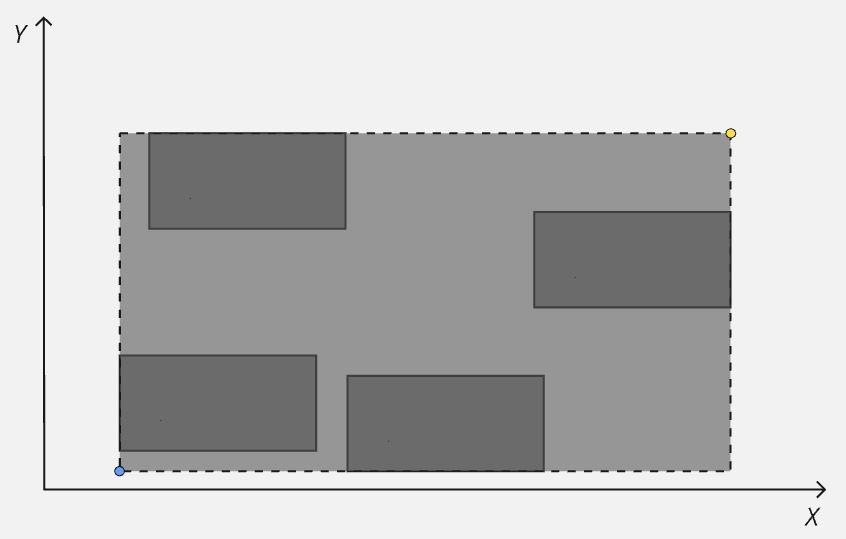
\includegraphics[width=0.6\textwidth]{figures/Orden/image.png}
  \caption{Representación gráfica del conjunto dominio de un mapa con 4 multi-intervalos, mas el marcado del mínimo y máximo perimetral en azul y amarillo resp.}
  \label{fig:minmaxPer1}
\end{figure}


Con toda esta información ya se puede declarar formalmente cómo está constituida la variable \texttt{pieces\_} para los \textit{piecewise maps} ordenados, denominados como \texttt{OrdPWMap}:

\begin{itemize}
  \item \texttt{pieces} (de tipo \textbf{OrdMapCollection}): 
  representa la colección ordenada de mapas junto con la información perimetral 
  de sus dominios.  
  En este contexto:
  \begin{itemize}
    \item \texttt{OrdMapCollection} es sinónimo de \texttt{vector<MapEntry>}.
    \item \texttt{MapEntry}, cuyas instancias denominaremos en adelante \textit{entradas de mapa}, es sinónimo de \texttt{pair<Map, SetPerimeter>}.
    \item \texttt{SetPerimeter}, cuyas instancias denominaremos en adelante \textit{perímetros}, es sinónimo de \texttt{pair<MD\_NAT, MD\_NAT>}.
  \end{itemize}
\end{itemize}


Y por ultimo se presenta el siguiente ejemplo. Sean se los siguientes conjuntos dominio de los mapas $m_1$, $m_2$, y $m_3$ respectivamente:

\begin{itemize}
    \item $c_1 = \{|[10:1:15]\times[10:1:11]|,||[16:1:20]\times[15:1:20]|\}$, con mínimo perimetral $(10,10)$
    \item $c_2 = \{|[15:1:20]\times[15:1:25]|,||[21:1:25]\times[15:1:20]|\}$, con mínimo perimetral $(15,15)$
    \item $c_3 = \{|[30:1:35]\times[15:1:20]|,||[36:1:40]\times[10:1:11]|\}$, con mínimo perimetral $(30,10)$
\end{itemize}

Aplicando el criterio de orden basado en los mínimos perimetrales, junto con el operador $<$ definido para la naturales multi-dimensionales, se obtiene el siguiente ordenamiento:

\begin{center}
\[
c_1 < c_2 < c_3
\]

ya que:

\[
(10,10) < (15, 15) < (30, 10)
\]

Por lo tanto, el conjunto ordenado resultante será:

\[
\ll (m_1,(minPer_1, maxPer1)),\ (m_2,(minPer_2, maxPer2)),\ (m_3, (minPer_3, maxPer3))\gg
\]
\end{center}


\section{\textit{Abstarct factory} para estructuras ordenadas}

Al igual que se hizo con los conjuntos desordenados y ordenados densos, 
así como con los \textit{piecewise maps} desordenados, 
también se definieron las fábricas concretas para los conjuntos ordenados 
y para los \textit{piecewise maps} ordenados, en el marco de las dos 
instancias del patrón de diseño \textit{Abstract Factory}. 

En particular, la fábrica concreta de los conjuntos ordenados se denominó 
\texttt{OrdAF}, mientras que la correspondiente a los 
\textit{piecewise maps} ordenados recibió el nombre de \texttt{OrdPWMapAF}. 
Ambas implementaciones pueden encontrarse en los archivos 
\textit{af\_set} y \textit{af\_pwmap}, tanto en sus versiones 
\textit{.cpp} como \textit{.hpp}, dentro de la carpeta \texttt{sbg} 
del repositorio~\cite{sbg}.

%\chapter{Criterios de optimización y ordenamiento para conjuntos ordenados}

En este capítulo se describen en detalle los diferentes \textbf{criterios de optimización}, así como los \textbf{criterios de ordenamiento} empleados en las operaciones para conjuntos ordenados. Ambos conjuntos de criterios se aplicarán posteriormente con el objetivo de mejorar la eficiencia general de las operaciones y reducir significativamente los tiempos de ejecución.

Ahora bien, para que todo este claro, un criterio de optimización es en esencia un predicado que permite deduci

\textbf{Pseudocódigo y notación:} En este capítulo, al igual que se hizo para los conjuntos desordenados, se emplearán subíndices para referirse a los multi-intervalos de un conjunto ordenado. Dado un conjunto ordenado $A$, el elemento ubicado en la posición $i$, lo cual corresponde a \texttt{pieces\_[i]} en C++, se denotará como \textbf{$A_i$}, donde $i$ es un número natural que satisface $0 \leq i < |A|$, siendo $|A|$ el cardinal del conjunto $A$, es decir, la cantidad total de elementos que contiene. Cabe destacar que, al tratarse de un conjunto ordenado, siempre se cumple que $A_i < A_j$ si y sólo si $i < j$, para todo par de $i$ y $j$ tal que $0  \leq i, j < |A|$. Adicionalmente se dirá que, en el caso anterior $A_i$ esta \textbf{antes} de $A_j$ en $A$, mientras $A_j$ esta \textbf{después} de $A_i$

\section{Intersección - \texttt{intersection}}

La operación \texttt{intersection} constituye un componente central dentro de la batería de operaciones fundamentales para conjuntos. Antes de presentar las optimizaciones específicas y su correspondiente criterio de ordenamiento, es conveniente recordar el funcionamiento general de la intersección de conjuntos:

\begin{center}
\textit{Para intersecar dos conjuntos se debe considerar que cada conjunto está compuesto por multi-intervalos. Por lo tanto, la operación consiste en evaluar todas las posibles intersecciones de los multi-intervalos de uno de los conjunto con los del otro conjunto participante .}
\end{center}

Esto se puede ver en el pseudocódigo de la operación \texttt{intersección} para conjuntos desordenados ~\ref{alg:interseccionDes}.
\subsection{Criterios de optimización}

\subsubsection{Criterio de parada}

\begin{center}
    \textit{Supongase que se lleva a cabo la intersección entre $A$ y $B$, dos conjuntos ordenados, y se están considerando las posibles intersecciones del multi-intervalo \( i \)-ésimo de $A$, \( A_i \), con todos los multi-intervalos de $B$.}
\end{center}

\begin{figure}[h]
     \centering
    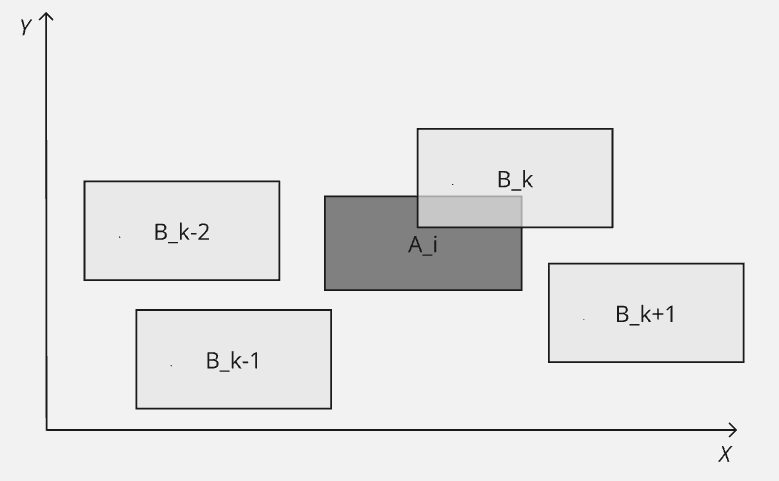
\includegraphics[width=0.75\linewidth]{figures/Optimazaciones/Interseccion/interseccion1a1.png}\par
    \caption{Ejemplificación de una iteración del proceso de intersección sobre dos conjuntos A y B.}
    \label{fig:enter-label}
\end{figure}

En algún punto, puede que se alcance un valor $k$, con $0 \leq k < |B|$, tal que el elemento mínimo de $B_k$ sea estrictamente mayor, en su primera dimensión (dimensión $x$ o $0$), que el elemento máximo de $A_i$. Por ejemplo, si el mínimo de $B_k$ es $(3,5)$ y el máximo de $A_i$ es  $(2,3)$. En este caso, se pueden derivar las siguientes conclusiones:

\begin{itemize}
     \item La intersección entre $A_i$ y $B_k$ resulta vacía, ya que como todos los valores de $A_i$ tienen un valor menor o igual que el máximo de $A_i$ en la primera dimensión, todos los valores de $B_k$ tienen un valor mayor o igual que el mínimo de $B_k$ en la primera dimensión y, como se vio, el elemento mínimo de $B_k$ sea estrictamente mayor en su primera dimensión que el elemento máximo de $A_i$, entonces ningún elemento de $A_i$ esta en $B_k$
    
    \item Debido al orden creciente de los conjuntos por el operador $<$ de multi-intervalos, cualquier multi-intervalo $B_{k'}$ con $k < k' < |B|$ tendrá en la primera dimensión de su mínimo un valor mayor o igual que el mínimo de $B_k$ en dicha dimensión, lo cual garantiza que también será vacía su intersección con $A_i$.
\end{itemize}

\begin{figure}[h]
    \centering
    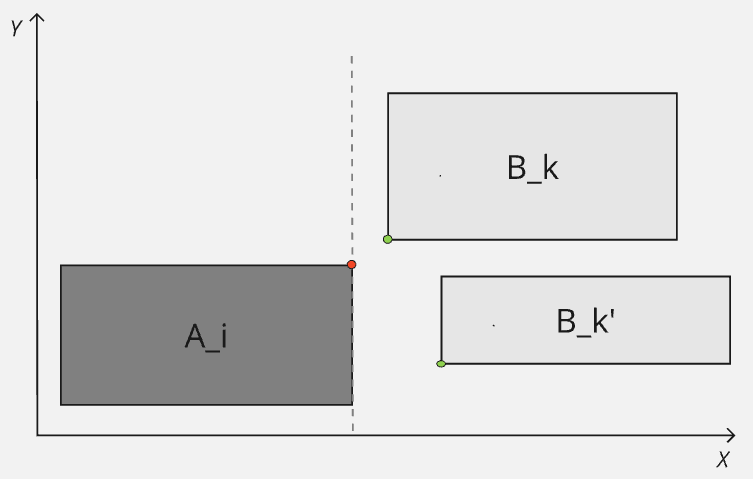
\includegraphics[width=0.75\linewidth]{figures/Optimazaciones/Interseccion/criterio de parada.png}
    \caption{Criterio de parada.}
    \label{fig:criterio-parada}
\end{figure}

En consecuencia, se puede establecer el siguiente criterio fundamental para optimizar la intersección entre conjuntos ordenados:

\begin{center}
    \fbox{
        \parbox{0.92\linewidth}{
            \centering
            \textbf{Criterio de parada} \\[1ex]
            \raggedright
            Sean $A$ y $B$ dos conjuntos ordenados. Supóngase que se está evaluando la intersección entre ambos, y en particular se consideran las posibles intersecciones entre un multi-intervalo $A_i$ de $A$, con $0 \leq i < |A|$, y los multi-intervalos de $B$. Dado un índice $k$ tal que $0 \leq k < |B|$, vale lo siguiente:

            \vspace{0,5cm}
     
            \textbf{Si} el máximo de $A_i$ es estrictamente menor que el mínimo de $B_k$ en la primera dimensión, \textbf{entonces}:

            \begin{itemize}
                \item la intersección entre $A_i$ y $B_{k'}$ resulta vacía, $\forall k' \mid k \leq k' < |B|$,
                \item \textbf{y, entonces} puede continuarse directamente con la evaluación de las intersecciones entre $A_{i+1}$(si existe) y los elementos de $B$ al no aceptar los conjuntos multi-intervalos vacíos.
            \end{itemize}
    
        }
    }
\end{center}

\subsubsection{Criterio de eliminación}

\begin{center}
    \textit{Nuevamente, supongase que se lleva a cabo la intersección entre $A$ y $B$, dos conjuntos ordenados, y se están considerando las posibles intersecciones del multi-intervalo \( i \)-ésimo de $A$, \( A_i \), con todos los multi-intervalos de $B$.}
\end{center}

En algún punto, puede que se alcance un valor $k$, con $0 \leq k < |B|$, tal que el elemento máximo de $B_k$ sea estrictamente menor, en su primera dimensión (dimensión $x$ o $0$), que el elemento mínimo de $A_i$. Por ejemplo, si el mínimo de $A_i$ es $(3,5)$ y el máximo de $B_k$ es  $(2,3)$. En este caso, se pueden derivar las siguientes conclusiones:

\begin{itemize}
     \item La intersección entre $A_i$ y $B_k$ resulta vacía, ya que como todos los valores de $A_i$ tienen un valor mayor o igual que el mínimo de $A_i$ en la primera dimensión, todos los valores de $B_k$ tienen un valor menor o igual que el máximo de $B_k$ en la primera dimensión y, como se vio, el elemento máximo de $B_k$ sea estrictamente menor en su primera dimensión que el elemento mínimo de $A_i$, entonces ningún elemento de $A_i$ esta en $B_k$

    \item Debido al orden creciente de los conjuntos por el operador $<$ de multi-intervalos, cualquier multi-intervalo $A_{i'}$ con $i < i' < |A|$ tendrá en la primera dimensión de su mínimo un valor mayor o igual que el mínimo de $A_i$ en dicha dimensión, lo cual garantiza que también será vacía su intersección con $B_k$.
\end{itemize}

\begin{figure}[h]
    \centering
    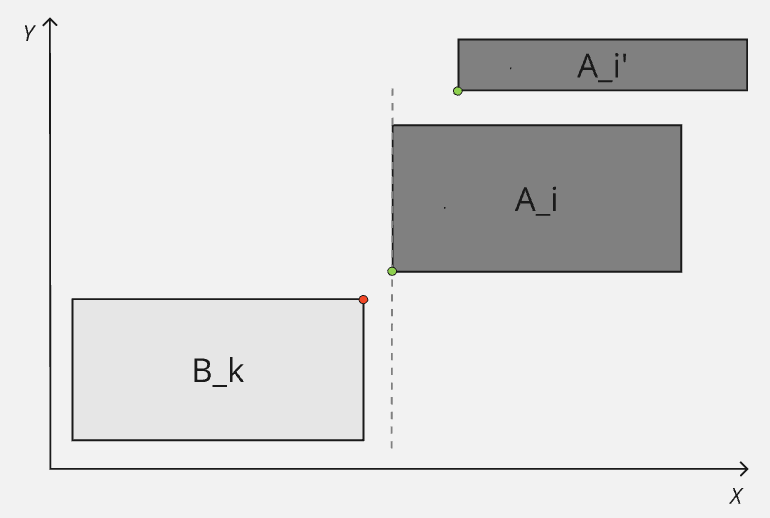
\includegraphics[width=0.75\linewidth]{figures/Optimazaciones/Interseccion/criterio de elim.png}
    \caption{Criterio de eliminación.}
    \label{fig:criterio-eliminacion}
\end{figure}

En consecuencia, se puede establecer el siguiente criterio fundamental para optimizar la intersección entre conjuntos ordenados:


\begin{center}
    \fbox{
        \parbox{0.92\linewidth}{
            \centering
            \textbf{Criterio de eliminación} \\[1ex]
            \raggedright
            Sean $A$ y $B$ dos conjuntos ordenados. Supóngase que se está evaluando la intersección entre ambos, y en particular se consideran las posibles intersecciones entre un multi-intervalo $A_i$ de $A$, con $0 \leq i < |A|$, y los multi-intervalos de $B$. Dado un índice $k$ tal que $0 \leq k < |B|$, vale lo siguiente:

            \vspace{0,5cm}
     
            \textbf{Si} el máximo de $B_k$ es estrictamente menor que el mínimo de $A_i$ en la primera dimensión, \textbf{entonces}:

            \begin{itemize}
                \item la intersección entre $A_{i'}$ y $B_{k}$ resulta vacía, $\forall i' \mid i \leq i' < |A|$,
                
                \item \textbf{y, entonces} puede descartarse $B_k$ para los cálculos de las posibles intersecciones de los multi-intervalos posteriores a $A_i$ al no aceptar los conjuntos multi-intervalos vacíos.
            \end{itemize}
    
        }
    }
\end{center}

Cabe señalar que, tanto para este criterio como para el anterior, no se especifica el tipo de multi-intervalo (si es denso o no), ya que dicha característica no afecta directamente la validez de los mismos.


\subsubsection{Criterio de selección}

Como se analizó en el criterio de eliminación, el procedimiento de intersección considera cada multi-intervalo del conjunto $A$ e intenta intersectarlo con todos los multi-intervalos del conjunto $B$. Y donde la idea central del criterio es que, a medida que se avanza en este proceso, ciertos elementos de $B$ pueden ser descartados progresivamente si se determina que ya no podrán intersectar con los siguientes elementos de $A$.

Naturalmente, se puede llegar al punto en el cual todos los elementos de $B$ habrán sido descartados, lo que implica que la operación \texttt{intersection} podrá finalizar directamente ya que no quedan intersecciones posibles a verificar.

Ahora bien, existe una observación importante respecto al tamaño de $B$: cuanto menor sea la cantidad de multi-intervalos en $B$, más rápido podrán descartarse todos ellos posiblemente, y por tanto, terminar la operación.

En base a esta idea, se introduce el \textbf{criterio de selección}, el cual establece lo siguiente:

\begin{center}
    \fbox{
        \parbox{0.9\linewidth}{
            \centering
            \textbf{Criterio de selección} \\[1ex]
            \raggedright
            Sean dos conjuntos ordenados involucrados en la operación de intersección. Se establece lo siguiente:

            \begin{center}
            \textit{
                Se define como $B$ a aquel conjunto que contiene la menor cantidad de multi-intervalos,
                mientras que se denota como $A$ al conjunto restante.
            }
            \end{center}
        }
    }
\end{center}

\subsubsection{Criterio de solapamiento}


Se introduce ahora el \textbf{criterio de solapamiento}, el cual establece lo siguiente:

\begin{center}
    \fbox{
        \parbox{0.93\linewidth}{
            \centering
            \textbf{Criterio de solapamiento} \\[1ex]
            \raggedright
            Sean $A$ y $B$ dos conjuntos, $A_i$ un multi-intervalo del conjunto $A$ y $B_k$ un multi-intervalo del conjunto $B$, con índices tales que:
            \[
            0 \leq i < |A|, \quad 0 \leq k < |B|.
            \]
            Se establece entonces que, en el caso de realizar la intersección entre $A$ y $B$:

            \begin{itemize}
                \item \textbf{Si} existe solapamiento entre $A_i$ y $B_k$, \textbf{entonces}:
                \begin{itemize}
                    \item \textbf{Si} ambos multi-intervalos son \textit{densos}, la intersección entre ellos es necesariamente no vacía y debe proceder.
                    \item \textbf{Si} al menos uno de ellos no es denso, la intersección \textit{puede} ser no vacía, pero no se garantiza de modo que se debe proceder de igual manera.
                \end{itemize}

                \item \textbf{Si} \textbf{no} existe solapamiento entre $A_i$ y $B_k$, \textbf{entonces} la intersección entre ellos es necesariamente vacía, independientemente de si son densos o no, y por ende puede obviarse su calculo.
            \end{itemize}
        }
    }
\end{center}

Ahora bien, seguiría explicar que es el solapamiento en si:

\begin{center}
    \textit{Sean dos multi-intervalos $m_1$ y $m_2$. Los multi-intervalos $m_1$ y $m_2$ se \textbf{solapan} \textbf{si}, \textbf{y sólo si}, todos sus intervalos componentes en cada dimensión se solapan.}

    \textit{Sean $a = [a_{\text{begin}} : a_{\text{step}} : a_{\text{end}}]$ y $b = [b_{\text{begin}} : b_{\text{step}} : b_{\text{end}}]$ dos intervalos. Se dice que se \textbf{solapan} \textbf{si}, \textbf{y sólo si}, se cumple alguna de las siguientes condiciones:}

$\neg (b_{\text{end}} < a_{\text{begin}} \lor a_{\text{end}} < b_{\text{begin}})$
\end{center}

Para ejemplificar mejor la noción de solapamiento en intervalos se proponen los siguientes casos en base a la predicado presentado por la definición:

\begin{itemize}
    \item \textbf{Primer caso:} Se cumple que $b_{\text{end}} < a_{\text{begin}}$ y $a_{\text{end}} < b_{\text{begin}}$ no.

    En este caso, no hay solapamiento. Por ejemplo, si $b = [1:1:5]$ y $a = [6:2:10]$, entonces $5 < 6$, por lo tanto, no se solapan.

    \begin{figure}[h]
        \centering
        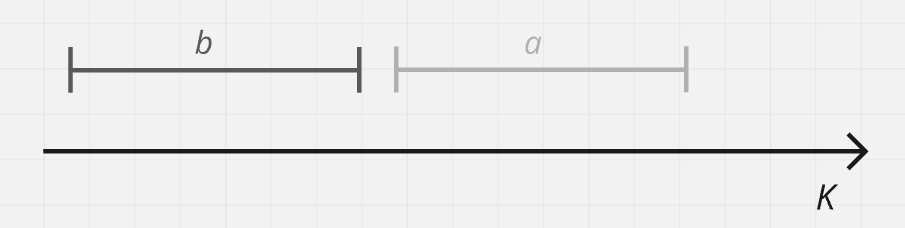
\includegraphics[width=0.75\linewidth]{figures/Optimazaciones/Interseccion/crit sol 10.png}
        \caption{Solapamiento sobre intervalos: \textit{primera condición verdadera}.}
    \end{figure}

    \item \textbf{Segundo caso:} No se cumple que $b_{\text{end}} < a_{\text{begin}}$ pero $a_{\text{end}} < b_{\text{begin}}$ si.

    Nuevamente, no hay solapamiento. Por ejemplo, si $b = [8:2:10]$ y $a = [4:2:6]$, entonces $6 < 8$.

    \begin{figure}[h]
        \centering
        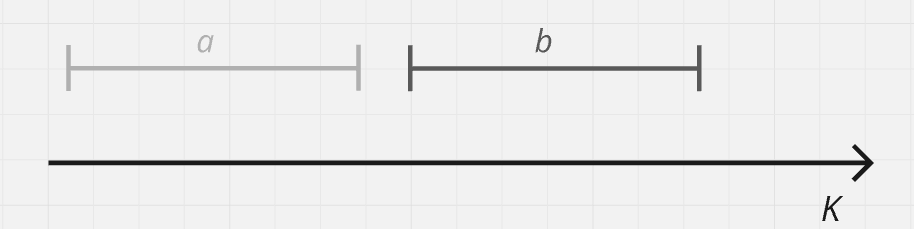
\includegraphics[width=0.75\linewidth]{figures/Optimazaciones/Interseccion/crit sol01.png}
        \caption{Solapamiento sobre intervalos: \textit{segunda condición verdadera}.}
    \end{figure}

    \item \textbf{Tercer caso:} Ninguna de las dos condiciones se cumple.

    En este caso resulta que se pueden dar dos situaciones unicamente: $b_{begin}$ o $b_{end}$ se encuentran entre $a_{begin}$ y $a_{end}$ inclusive(Figura~\ref{fig:crit-solapamiento-b}, Figura~\ref{fig:crit-solapamiento-c} y Figura~\ref{fig:crit-solapamiento-d}), ó $b_{begin} < a_{begin}$ y $b_{end}>a_{end}$(Figura~\ref{fig:crit-solapamiento-a}).

\begin{figure}[H]
    \centering

    \begin{subfigure}{0.75\linewidth}
        \centering
        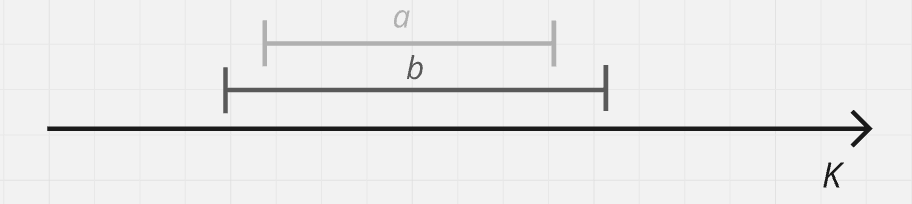
\includegraphics[width=\linewidth]{figures/Optimazaciones/Interseccion/crit sol 11 1.png}
        \caption{}
        \label{fig:crit-solapamiento-a}
    \end{subfigure}
    
    \vspace{0.4cm}

    \begin{subfigure}{0.75\linewidth}
        \centering
        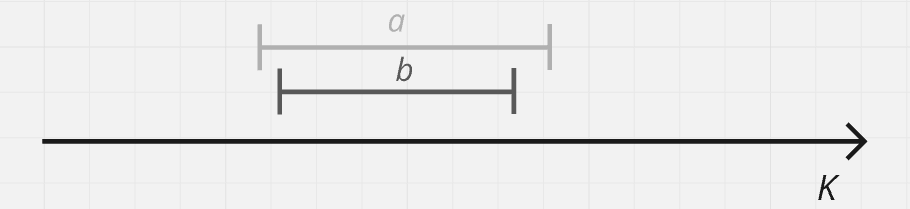
\includegraphics[width=\linewidth]{figures/Optimazaciones/Interseccion/crit sol 11 2.png}
        \caption{}
        \label{fig:crit-solapamiento-b}
    \end{subfigure}
    
    \vspace{0.4cm}

    \begin{subfigure}{0.75\linewidth}
        \centering
        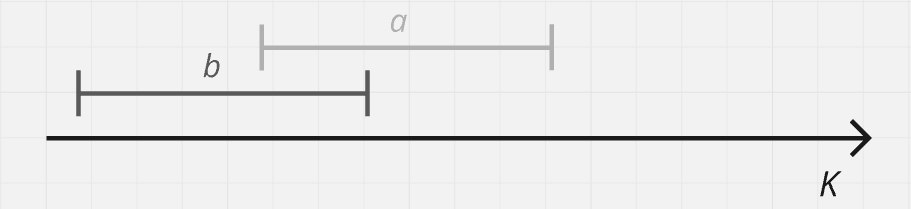
\includegraphics[width=\linewidth]{figures/Optimazaciones/Interseccion/crit sol 11 3.png}
        \caption{}
        \label{fig:crit-solapamiento-c}
    \end{subfigure}
    
    \vspace{0.4cm}

    \begin{subfigure}{0.75\linewidth}
        \centering
        \includegraphics[width=\linewidth]{figures/Optimazaciones/Interseccion/crit sol 11 4.png}
        \caption{}
        \label{fig:crit-solapamiento-d}
    \end{subfigure}

    \caption{Solapamiento sobre intervalos: \textit{el predicado entero es falso}.}
    \label{fig:crit-solapamiento}
\end{figure}
        \item \textbf{Cuarto caso:} Las dos condiciones se cumplen.
        
        Cabe destacar que el caso en el cual \textbf{ambas condiciones} sean verdaderas simultáneamente es imposible. En efecto, si se cumple que:

        \[
        b_{\text{end}} < a_{\text{begin}} \quad \text{y} \quad a_{\text{end}} < b_{\text{begin}},
        \]
        
        entonces, por $a_{\text{begin}} < a_{\text{end}}$ y transitividad de la desigualdad, se deduce que:
        
        \[
        b_{\text{end}} < b_{\text{begin}},
        \]
        
        lo cual implicaría que el intervalo $b$ está mal definido, ya que su extremo final es menor que su extremo inicial. Esto contradice la definición válida de intervalo, por lo tanto, dicho caso \textbf{no} puede ocurrir.
\end{itemize}


Por un lado, se puede observar que si, en al menos una dimensión, los intervalos correspondientes de dos multi-intervalos $m$ y $p$, ya sean densos o no, no se solapan, entonces no existe ninguna $n$-upla $(m_0, \dots, m_{n-1}) \in m$ y $(p_0, \dots, p_{n-1}) \in p$ tal que coincidan en esa dimensión, con $n$ siendo la aridad de $m$ y $p$. En consecuencia, esto implica que la intersección entre $m$ y $p$ será vacía, independientemente de que en las demás dimensiones sí exista solapamiento.

Por otro lado, si en todas las dimensiones los intervalos correspondientes se solapan y ambos multi-intervalos son densos, entonces se garantiza la existencia de al menos una $n$-upla $(m_0, \dots, m_{n-1})$ perteneciente tanto a $m$ como a $p$. En efecto, basta con elegir un valor dentro del intervalo intersección para cada dimensión, lo cual es posible precisamente porque los intervalos son densos y contienen todos los valores posibles del $begin$ al $end$.

Sin embargo, si uno o ambos multi-intervalos no son densos, esta garantía desaparece. Aunque exista solapamiento en todas las dimensiones, podría no haber ninguna $n$-upla común, ya que en alguna dimensión podría ocurrir que, debido al paso distinto de 1, el intervalo solapamiento puede no tener valores a partir de los cuales elegir. Por ejemplo, en una dimensión se pueden contar con los intervalos $[5:5:10]$ y $[6:1:9]$, los cuales se solapan pero cuyo intervalo intersección es vació. 

\subsection{Criterio de ordenamiento}

Uno de los aspectos fundamentales a considerar al implementar la operación de intersección entre conjuntos ordenados es cómo construir el conjunto resultado de manera que conserve su orden intrínseco. En este contexto, el desafío consiste en insertar las intersecciones de los multi-intervalos en el conjunto resultado de la forma más eficiente posible, garantizando siempre que se mantenga la invariante del orden.

\begin{center}
    \fbox{
        \parbox{0.93\linewidth}{
            \centering
            \textbf{Criterio de ordenamiento} \\[1ex]
            \raggedright
            Supóngase que se realiza la intersección entre dos conjuntos ordenados, $A$ y $B$, y que se están evaluando las posibles intersecciones del $i$-ésimo multi-intervalo de $A$, denotado por $A_i$, con todos los multi-intervalos de $B$. Ademas se cuenta con un conjunto resultado $C$.

            \vspace{1ex}

            Todas las intersecciones no vacías generadas con $A_i$ deben insertarse en $C$ \textbf{después} de aquellas intersecciones generadas por los multi-intervalos $A_0, A_1, \dots, A_{i-1}$, cuyos mínimos sean estrictamente menores al de $A_i$, bajo el operador $<$ de naturales multi-dimensionales.
        }
    }
\end{center}


Este criterio se fundamenta en la observación de que la intersección entre dos multi-intervalos está contenida en ambos. Esto implica que el elemento mínimo de la intersección debe ser, necesariamente, un valor que pertenezca a ambos operandos, y por lo tanto debe coincidir con el mínimo de alguno de ellos, o bien ser un valor contenido en ambos.

Al fijar el multi-intervalo $A_i$ como decreta el criterio, se observa que cualquier intersección no vacía con un multi-intervalo $B_k$ del conjunto $B$ tendrá su mínimo dentro de $A_i$, o coincidirá con el mínimo de este. Como resultado, cualquier intersección no vacía generada tendrá un mínimo mayor, bajo el operador $<$ de naturales multi-dimensionales, o igual que el mínimo de $A_i$.

Esto garantiza que tales intersecciones deben insertarse en el conjunto resultado después de aquellas cuyo mínimo sea estrictamente menor, bajo el operador $<$ de naturales multi-dimensionales, al de $A_i$. 

La Figura~\ref{fig:enter-label} ilustra gráficamente esta situación. Como se observa, todas las intersecciones producidas a partir de $A_i$ tienen un mínimo mayor o igual que el de $A_i$, y se insertan a continuación de las intersecciones previamente procesadas cuyo mínimo sea menor al de $A_i$. Esto mismo ocurre con las de $A_{i+1}$

\begin{figure}[h]
    \centering
    \includegraphics[width=0.7\linewidth]{figures/Optimazaciones/Interseccion/crit ordenamiento.png}
    \caption{Criterio de ordenamiento en la intersección de conjuntos ordenados.}
    \label{fig:enter-label}
\end{figure}

Adicionalmente, no es necesario comenzar a verificar la posición de inserción de las intersecciones en el conjunto resultado desde el principio en cada iteración de los elementos de $A$. Dado el orden intrínseco de los conjuntos involucrados, se cumple que:
\begin{center}
    \textit{El mínimo de $A_i$ es menor, bajo el operador $<$ de naturales multi-dimensionales, al mínimo de $A_{i+1}$}
\end{center}

Esto implica, en conjunto con lo establecido previamente sobre los mínimos de las intersecciones generadas, que todas las intersecciones obtenidas a partir de $A_{i+1}$ con los elementos de $B$ deben insertarse en el conjunto resultado a partir de una posición \textbf{igual o posterior} a aquella en la que comenzaron a insertarse las intersecciones de $A_i$ con $B$.

Por lo tanto, el criterio de ordenamiento puede refinarse del siguiente modo:



\begin{center}
    \fbox{
        \parbox{0.93\linewidth}{
            \centering
            \textbf{Criterio de ordenamiento} \\[1ex]
            \raggedright
            Supóngase que se realiza la intersección entre dos conjuntos ordenados, $A$ y $B$, y que se están evaluando las posibles intersecciones del $i$-ésimo multi-intervalo de $A$, denotado por $A_i$, con todos los multi-intervalos de $B$. Ademas se cuenta con un conjunto resultado $C$.

            \vspace{1ex}

            Todas las intersecciones no vacías generadas con $A_i$ deben insertarse en $C$ \textbf{después} de aquellas intersecciones generadas por los multi-intervalos $A_0, A_1, \dots, A_{i-1}$, cuyos mínimos sean estrictamente menores al de $A_i$, bajo el operador $<$ de naturales multi-dimensionales.
            
            \vspace{1ex}

            Adicionalmente \textbf{si} la posición a partir de la cual se colocan las intersecciones de $A_i$ en el conjunto resultante es $k$, con $0 \leq k < |C|$, \textbf{entonces} aquellas generadas por $A_{i+1}$ se insertaran a partir de $k'$ tal que $k \leq k' < |C|$.
        }
    }
\end{center}



Esta optimización reduce significativamente la cantidad de comparaciones necesarias para ubicar cada intersección, manteniendo la eficiencia del proceso y evitando retrocesos innecesarios dentro de la estructura del conjunto ordenado resultante.


\section{Unión disjunta - \texttt{disjointCup}}

La operación \texttt{disjointCup} se encarga de realizar la unión disjunta entre dos conjuntos de multi-intervalos que, por hipótesis, son disjuntos. En particular, esta operación simplemente coloca los elementos de ambos conjuntos en uno solo, sin aplicar ningún tipo de transformación adicional ni sobre los argumentos ni sobre el contenido de sus elementos. Esto se puede ver muy bien particularmente en el pseudocódigo de esta para conjuntos desordenados \ref{alg:disjointcupDes}.

Ahora bien, al trabajar con conjuntos \textit{ordenados}, resulta necesario introducir un criterio de ordenamiento que garantice que el conjunto resultante mantenga el orden. Este criterio de ordenamiento se presenta a continuación.

\subsection{Criterio de ordenamiento}

Dado que la función \texttt{disjointCup} se encarga de realizar la fusión de dos conjuntos ordenados en esta ocasión, es fundamental establecer con claridad el \textbf{criterio de ordenamiento}.

\begin{center}
    \fbox{
        \parbox{0.93\linewidth}{
            \centering
            \textbf{Criterio de ordenamiento}\\[1ex]
            \raggedright
            Sean $A = \{A_0, A_1, \dots, A_{n-1}\}$ y $B = \{B_0, B_1, \dots, B_{m-1}\}$ dos conjuntos no vacíos de multi-intervalos, disjuntos y ordenados. Sea $C$ un conjunto ordenado que contendrá el resultado de la fusión de $A$ y $B$. Y sean $A_i$ un multi-intervalo del conjunto $A$ y $B_k$ un multi-intervalo del conjunto $B$, con índices tales que:
            \[
            0 \leq i < |A|, \quad 0 \leq k < |B|.
            \]
            
            \vspace{1ex}

            Entonces, al realizar la unión disjunta entre $A$ y $B$ vale que:

            \begin{itemize}
                \item \textbf{Si $A_i < B_k$}, entonces $A_i$ debe insertarse en $C$ \textbf{antes} que $B_k$.
                \item \textbf{Si $B_k < A_i$}, entonces $B_k$ debe insertarse en $C$ \textbf{antes} que $A_i$.
            \end{itemize}

            \vspace{1ex}
        }
    }
\end{center}

Como se puede ver, el criterio unicamente se basa en el orden intrínseco de los conjuntos y no es para nada complejo o enrevesado.

\section{Complemento - \texttt{complement / complementAtom}}

Esta sección se dividirá en dos partes, ya que la operación de complemento para conjuntos ordenados, al igual que su contraparte de conjuntos desordenados, se compone de dos etapas: el \textit{complemento atómico} (\texttt{complementAtom}), que calcula el complemento de un conjunto ordenado representado por un único multi-intervalo; y el \textit{complemento general} (\texttt{complement}), la operación principal del complemento, que extiende esta operación tal que sea posible calcular el complemento de conjuntos ordenados compuestos por múltiples multi-intervalos a través de la operación \texttt{intersection}.

\subsection{Complemento atómico(\texttt{complementAtom})}

En el capítulo de conceptos previos se presentó el funcionamiento y la lógica de la construcción del conjunto complemento de un conjunto atómico, un conjunto compuesto por un único multi-intervalo, mediante la operación \texttt{complementAtom}, en el contexto de los conjuntos desordenados.

Tal como se mencionó, la estructura general de la implementación de las operaciones para conjuntos ordenados se basa en la utilizada para conjuntos desordenados. Por esta razón, correspondería ahora optimizar dicha operación teniendo en cuenta el orden y adaptarla para conjuntos ordenados.

Sin embargo, dado que el conjunto base contiene únicamente un multi-intervalo y solo contamos con un único conjunto como argumento de la operación, no hay margen para aplicar ninguna optimización basada en el orden de los argumentos de entrada. 

Por lo tanto, la única tarea pendiente es poder construir un conjunto ordenado resultado, lo cual implica determinar el \textbf{criterio de ordenamiento}.

\subsubsection{Criterio de ordenamiento}

En \texttt{complementAtom} se trabaja con dos tipos de multi-intervalos: \textit{all} y \textit{during}. Las transformaciones sucesivas de estos intervalos conforman el complemento del conjunto atómico. El uso de cada uno es el siguiente:

Sea $i$ un numero natural que hace referencia una dimensión entre $0$ y la cantidad de dimensiones del conjunto atómico procesado.
\begin{itemize}
  \item \textbf{\textit{all}}:  
    Construye el multi-intervalo ($\textit{all}_{i,b}$) que va desde $0$ hasta el inicio del multi-intervalo del conjunto en la dimensión $i$, siempre que exista.

  \item \textbf{\textit{during}} :  
    Cuando el multi-intervalo del conjunto no es denso en la dimensión $i$, es decir, el paso de la $i$-esima dimensión ($\text{paso}_i$) es distinto de $1$, se generan una serie de multi-intervalos intermedios ($\textit{during}_{i,c}$). Cada uno arranca en
    \[
      \bigl(\text{begin}_i\bigr) + c,
      \quad c = 1, 2, \dots, (\text{paso}_i - 1),
    \]
    donde $\text{begin}_i$ es el inicio en la dimensión $i$ del multi-intervalo del conjunto.

  \item \textbf{\textit{all}} :  
    Construye el multi-intervalo ($\textit{all}_{i,e}$) que va desde el final del multi-intervalo del conjunto en la dimensión $i$ hasta \texttt{Inf}, siempre que sea posible.
\end{itemize}

Sin embargo, al realizar el procesamiento secuencial de cada dimensión, es necesario tener en cuenta cómo los inicios de los intervalos correspondientes a las dimensiones ya recorridas del multi-intervalo  se propagan hacia $all$ y $during$. 

Una vez completados los cálculos en la dimensión $j$ (creación de \textit{all}$_{j,b}$, \textit{all}$_{j,e}$ y todos los \textit{during}$_{j,c}$), tanto \textit{during} como \textit{all} se modifican en dicha dimensión. A \textit{all} se le remplaza el intervalo en esa dimensión por el del multi-intervalo del conjunto en la misma dimensión pero con paso 1, y a \textit{during} se le hace lo mismo pero con el intervalo original.

Como consecuencia, todos los multi-intervalos que se generen en la siguiente dimensión $j+1$ tienen el mismo valor de inicio en la dimensión $j$ que tiene el multi-intervalo del conjunto. Por lo tanto los inicios de \textit{all}$_{i,b}$, \textit{all}$_{i,e}$ y de cada \textit{during}$_{i,c}$ coinciden, en las dimensiones $0,1,\ldots,i-1$, con los del multi-intervalo atómico original. Lo que conlleva a que el siguiente conjunto este ordenado:

\[
\{\textit{all}_{i,b},\;\textit{during}_{i,1},\;\textit{during}_{i,2},\;\dots,\;\textit{during}_{i,k},\;\textit{all}_{i,e}\}
\]

Pero ahora queda ver que interacción hay entre los conjuntos de cada dimensión para ver como ordenar la totalidad de los multi-intervalos de todas las dimensiones en un único conjunto.

Al estar en una dimensión $i$ y al haber terminado de generar los multi-intervalos de esa dimensión a través de \textit{during} y \textit{all}, por como son las modificaciones a estos dos multi-intervalos, resulta que todos los multi-intervalos generados en la dimensión $i+1$ van inmediatamente después de $all_{i,b}$(si existe), ya que en la dimensión $i$ tiene un valor de inicio $0$; y antes de los \textit{during}$_{i,c}$, cuyo inicio en la dimensión $i$ es el mismo que el de los multi-intervalos generados en $i+1$ pero mas una constante $c$. Como resultado tenemos que se da el siguiente orden:

\begin{align*}
\{ &\textit{all}_{x,b},\ \textit{all}_{y,b},\ \textit{all}_{z,b}, \\
   &\textit{during}_{z,1},\ \textit{during}_{z,2},\ \dots,\ \textit{during}_{z,k}, \\
   &\textit{all}_{z,e},\ \textit{during}_{y,1},\ \textit{during}_{y,2},\ \dots,\ \textit{during}_{y,j}, \\
   &\textit{all}_{y,e},\ \textit{during}_{x,1},\ \textit{during}_{x,2},\ \dots,\ \textit{during}_{x,j}, \\
   &\textit{all}_{x,e} \}
\end{align*}

trabajando con un conjunto atómico de tres dimensiones.

A partir de todo lo analizado previamente, se arriba a la siguiente formulación del criterio de ordenamiento para \texttt{complementAtom}:

\begin{center}
    \fbox{
        \parbox{0.93\linewidth}{
            \centering
            \textbf{Criterio de ordenamiento}\\[1ex]
            \raggedright
            El patrón general de inserción en las estructuras auxiliares $all$ y $during$, al recorrer las dimensiones en orden creciente, responde a la siguiente disposición:

            \begin{align*}
            \{ &\textit{all}_{0,b},\ \textit{all}_{1,b},\ \dots,\ \textit{all}_{d-1,b}, \\
               &\textit{during}_{d-1,1},\ \dots,\ \textit{during}_{d-1,k_{d-1}}, \\
               &\textit{all}_{d-1,e},\ \textit{during}_{d-2,1},\ \dots,\ \textit{during}_{d-2,k_{d-2}}, \\
               &\quad\vdots \\
               &\textit{all}_{1,e},\ \textit{during}_{0,1},\ \dots,\ \textit{during}_{0,k_0}, \\
               &\textit{all}_{0,e} \}
            \end{align*}

            \vspace{1ex}

            donde $d$ representa la aridad del conjunto (es decir, la cantidad de dimensiones), y $k_i$ indica la cantidad de pasos definidos en la dimensión $i$.
        }
    }
\end{center}



\subsection{Complemento general}

La operación \texttt{intersection} se utiliza como herramienta para calcular el complemento entre dos conjuntos desordenados en la operación \texttt{complement}: uno que representa el complemento de un conjunto de multi-intervalos desordenados, y otro que representa el complemento de un conjunto con un único multi-intervalo.

Teóricamente, podría utilizarse una única implementación general de \texttt{intersection}, como se hace en el caso de conjuntos desordenados y no modificar \texttt{complement} para el caso de conjuntos ordenados. Sin embargo, al tratarse de conjuntos ordenados, es posible aplicar ciertas optimizaciones adicionales, además de las ya detalladas en la sección correspondiente a \texttt{intersection}, que permiten mejorar el rendimiento de la operación. Es decir, se utilizara una versión adaptada de la intersección de conjuntos para el complemento.

\subsubsection{Intersección complementaria}

En esta modificación de la operación de intersección, denominada \texttt{intersectionComp}, se preservan los criterios de \textbf{parada}, \textbf{eliminación}, \textbf{solapamiento} y \textbf{ordenamiento}. Además de suponer que los conjuntos recibidos están ordenados, esta variante introduce una hipótesis adicional: los argumentos deben respetar un orden específico. El primer conjunto debe representar el complemento de un conjunto de multi-intervalos (posiblemente varios), mientras que el segundo conjunto corresponde al complemento de un único multi-intervalo. 

En otras palabras:
\begin{itemize}
    \item El primer conjunto, que denotara $A$, actúa como un \emph{complemento acumulado}.
    \item El segundo conjunto, denotado $B$, funciona como un \emph{complemento unitario}.
\end{itemize}

\textbf{Importante:} Para facilitar la siguiente explicación, se asume que los multi-intervalos involucrados son siempre densos.

Supongase ahora que el conjunto $A$ representa el complemento de un único multi-intervalo, al igual que $B$. Esta situación se ilustra en la Figura~\ref{fig:tra}.

\begin{figure}[htbp]
    \centering
    \begin{minipage}[t]{0.49\textwidth}
        \centering
        \includegraphics[width=\linewidth]{figures/Optimazaciones/Complement/Aelem.png}
        \caption*{\small Multi-intervalo generador de $A$}
        \vspace{8pt}
        \includegraphics[width=\linewidth]{figures/Optimazaciones/Complement/Belem.png}
        \caption*{\small Multi-intervalo generador de $B$}
    \end{minipage}%
    \hspace{0.01\textwidth}
    \begin{minipage}[t]{0.49\textwidth}
        \centering
        \includegraphics[width=\linewidth]{figures/Optimazaciones/Complement/A.png}
        \caption*{\small Conjunto complemento $A$}
        \vspace{8pt}
        \includegraphics[width=\linewidth]{figures/Optimazaciones/Complement/B.png}
        \caption*{\small Conjunto complemento $B$}
    \end{minipage}
    \caption{Ejemplo gráfico de los conjuntos complemento de $A$ y $B$.}
    \label{fig:tra}
\end{figure}

Si se aplicara directamente la operación \texttt{intersection}, utilizando su versión optimizada para conjuntos ordenados, el resultado obtenido sería el ilustrado en la Figura~\ref{fig:compleAnt}. 

Sin embargo, puede observarse que se produce una partición adicional innecesaria: los multi-intervalos $C\_1$ y $C\_3$ podrían haberse mantenido como un único multi-intervalo. Esta fragmentación/particionamiento es consecuencia del funcionamiento de la operación intersección. No obstante, ambos multi-intervalos no comparten ningún elemento con el multi-intervalo generador de $B$, por lo que no deberían verse afectados ni sufrir ninguna sustracción de elementos al quitar de $A$ los elementos del multi-intervalo generador de $B$ a través de la intersección de $A$ y $B$.


\begin{figure}[htbp]
    \centering
    \includegraphics[width=0.8\linewidth]{figures/Optimazaciones/Complement/complAnt.png}
    \caption{Conjunto complemento resultante de la intersección entre $A$ y $B$, sin aplicar optimización.}
    \label{fig:compleAnt}
\end{figure}

Este tipo de fragmentación innecesaria puede evitarse mediante el \textbf{criterio de anti-particionamiento}, que establece lo siguiente:

\begin{center}
    \fbox{
        \parbox{0.93\linewidth}{
            \centering
            \textbf{Criterio de anti-particionamiento} \\[1ex]
            \raggedright
            Sea $A$ un conjunto complemento y $B$ el complemento de un conjunto compuesto por un único multi-intervalo $m$. Al realizar la intersección entre $A$ y $B$ durante el cálculo del complemento de un conjunto, se cumple que:
            
            \vspace{1ex}
            Todo multi-intervalo de $A$ que no se solape con el multi-intervalo $m$ generado por $B$ no requiere ser intersectado con los elementos de $B$, y debe copiarse directamente al conjunto resultado.
        }
    }
\end{center}


Aplicando este criterio, el conjunto complemento resultante se muestra en la Figura~\ref{fig:compleNue}, donde se observa una representación más compacta: se evita una partición innecesaria y se obtiene un conjunto más chico.

\begin{figure}[htbp]
    \centering
    \includegraphics[width=0.8\linewidth]{figures/Optimazaciones/Complement/complNue.png}
    \caption{Conjunto complemento resultante tras aplicar el criterio de anti-particionamiento.}
    \label{fig:compleNue}
\end{figure}

Cabe destacar que este criterio también es válido cuando se trabaja con multi-intervalos no densos, y resulta especialmente útil en esos casos, ya que evita múltiples operaciones de posicionamiento y comparación innecesarias.

Si bien la reducción en el número de multi-intervalos resultantes puede parecer ínfima, es importante tener en cuenta que en la operación \texttt{complement} se aplica de forma acumulativa esta reducción. Por lo tanto, reducir la cantidad de particiones en cada iteración tiene un efecto significativo en el rendimiento total, ya que disminuye la cantidad de elementos a recorrer y comparar en las iteraciones posteriores.

Existe además una mejora adicional que puede aplicarse a la operación de intersección en el contexto del complemento. Esta surge del modo en que se construye el complemento ordenado de un conjunto atómico, tal como se explicó en la subsección correspondiente del complemento atómico.

En dicha construcción, el primer multi-intervalo del complemento ordenado es $\textit{all}_{x,b}$. Este multi-intervalo es denso y se extiende hasta el infinito en todas sus dimensiones, con excepción de la primera, donde finaliza una posición antes del comienzo del multi-intervalo original que dio lugar al complemento.

Adicionalmente se cumple que la intersección entre cualquier multi-intervalo y uno denso, que lo contiene por completo, es simplemente el multi-intervalo contenido. Es decir, si un multi-intervalo $m$ está completamente contenido en otro multi-intervalo denso $n$, entonces la intersección entre $m$ y $n$ es igual a $m$.

A partir de las observaciones anteriores, puede establecerse el \textbf{criterio de obviedad}, el cual permite evitar cálculos innecesarios durante la intersección del complemento, y estipula lo siguiente:

\begin{center}
    \fbox{
        \parbox{0.93\linewidth}{
            \centering
            \textbf{Criterio de obviedad} \\[1ex]
            \raggedright
            Sea $A$ un conjunto complemento y $B$ el complemento de un conjunto compuesto por un único multi-intervalo $m$. Al realizar la intersección entre $A$ y $B$ durante el cálculo del complemento de un conjunto, se cumple que:

            \vspace{0,5cm}
            
            Todo multi-intervalo del conjunto $A$ cuyo máximo sea estrictamente menor en la primera dimensión que el mínimo multi-intervalo generador de $B$, $m$, puede incorporarse directamente al conjunto resultado de la intersección, sin necesidad de ser intersectado con los elementos de $B$.
        }
    }
\end{center}


\begin{comment}
    

\begin{figure}[htbp]
    \centering
    \begin{minipage}[t]{0.49\textwidth}
        \centering
        \includegraphics[width=\linewidth]{figures/Optimazaciones/Complement/Ao.png}
        \caption*{\small Conjunto complemento $A$}
    \end{minipage}%
    \hspace{0.01\textwidth}
    \begin{minipage}[t]{0.49\textwidth}
        \centering
        \includegraphics[width=\linewidth]{figures/Optimazaciones/Complement/Bo.png}
        \caption*{\small Conjunto complemento $B$}
    \end{minipage}
    \hspace{0.01\textwidth}
    \begin{minipage}[t]{0.49\textwidth}
        \centering
        \includegraphics[width=\linewidth]{figures/Optimazaciones/Complement/complO.png}
        \caption*{\small Conjunto complemento resultante de la intersección}
    \end{minipage}
    \caption{Ejemplo gráfico de los conjuntos complemento $A$ y $B$.}
    \label{fig:tra}
\end{figure} 
\end{comment}


Tal como fue planteado, el \textbf{criterio de obviedad} permite evitar las comparaciones e intersecciones entre determinados multi-intervalos del conjunto complemento $A$ y los elementos del conjunto complemento $B$, pero su alcance inicial es limitado: únicamente evita el procesamiento de los multi-intervalos de $A$ que sean estrictamente menores (en la primera dimensión) que el multi-intervalo generador de $B$ en una única invocación de la operación \texttt{intersectionComplement}.

Sin embargo, este criterio puede extenderse de forma significativa durante el proceso iterativo de la operación \texttt{complement}. Esto es posible gracias a la siguiente observación: los multi-intervalos que generan cada conjunto $B$ a lo largo de las distintas iteraciones provienen de un conjunto ordenado, por lo tanto, sus valores iniciales en la primera dimensión son no decrecientes. Dado que estos multi-intervalos se recorren en orden, cada nuevo multi-intervalo generador $B$ tendrá en la primera dimension un valor de inicio igual o mayor que el anterior. Y, por ende cada nuevo $\textit{all}_{x,b}$ del conjunto $B$ generado por un multi-intervalo contendrá a todos los anteriores $\textit{all}_{x,b}$.

Como consecuencia, una vez que un multi-intervalo de $A$ ha sido descartado por el criterio de obviedad en una iteración, puede descartarse definitivamente para todas las iteraciones subsiguientes, ya que siempre sera obviado por el criterio obviedad.

Esto permite trasladar dichos multi-intervalos directamente al resultado final de la operación \texttt{complement}, en lugar de seguirlos incorporando los en el calculo de las posteriores iteraciones.

Se procede entonces a declarar el \textbf{criterio de obviedad extendido}:

\vspace{10pt}

\begin{center}
    \fbox{
        \parbox{0.93\linewidth}{
            Sea $A$ un conjunto ordenado de multi-intervalos que representa el complemento acumulado en una iteración de la operación \texttt{complement} y $B$ el complemento de un conjunto compuesto por un único multi-intervalo de dicha iteración también.

            \vspace{0,5cm}
            
            Entonces, $A$ puede \textit{descomponerse} en dos subconjuntos disjuntos:
            \begin{itemize}
                \item $A\_o$: el subconjunto de multi-intervalos que son descartados por el criterio de obviedad en base a $B$ en dicha iteración, y que, por lo tanto, pueden ser incorporados directamente al resultado final sin necesidad de ser procesados en iteraciones posteriores;

                
                \item $A\_r$: el subconjunto restante, compuesto por los multi-intervalos que aún pueden ser particionados en iteraciones futuras, es decir, aquellos que no son descartados por el criterio de obviedad en base a $B$. Luego, la intersección se dará entre este conjunto y $B$ y su resultado sera el nuevo $A$.
            \end{itemize}
        }
    }
\end{center}

Este criterio permite ahorrar el recorrer los mismos elementos múltiples veces durante el calculo de la intersección e el complemento. Esto permite aumentar en gran medida la eficiencia de la operación.
%\chapter{Criterios de optimización y ordenamiento para \textit{piecewise maps} ordenados}

En este capítulo se describen en detalle los distintos \textbf{criterios de optimización} y \textbf{ordenamiento} utilizados en las operaciones sobre \textit{piecewise maps} ordenados. Ambos conjuntos de criterios serán aplicados con el propósito de mejorar la eficiencia general de dichas operaciones y reducir significativamente los tiempos de ejecución.

\textbf{Pseudocódigo y notación:} En este capítulo, al igual que se hizo para los \textit{piecewise maps} desordenados, se emplearán subíndices para referirse a los mapas de un \textit{piecewise map} ordenado con ele fin de alivianar la notación. Dado un \textit{piecewise map} ordenado $A$, el elemento ubicado en la posición $i$, lo cual corresponde a \texttt{pieces\_[i].first} en C++, se denotará como \textbf{$A_i$}, donde $i$ es un número natural que satisface $0 \leq i < |A|$, siendo $|A|$ la cantidad de mapas de $A$.

\section{Operaciones estructuralmente similares}

Como se puede ver en la sección de conceptos previos correspondiente a los \textit{piecewise maps} desordenados, existen muchas operaciones que presentan una estructura muy similar a la de la intersección entre conjuntos desordenados. Entre estas operaciones se encuentran: la \textbf{igualdad}, la \textbf{suma}, la i\textbf{gualdad de imágenes}, la \textbf{resta} y el \textbf{mínimo adyacente}.

Todas estas operaciones, junto con la intersección de conjuntos ordenados, comparten una estructura común que se puede dividir en dos partes: 
\begin{enumerate}
    \item Una\textbf{ fase de comparación}, donde cada elemento de uno de los argumentos es comparado con todos los del otro argumento.
    \item Un \textbf{núcleo de la operación}, donde se ejecuta la lógica específica de la operación sobre aquellos pares de elementos cuya comparación fue satisfactoria.
\end{enumerate}

Esta estructura puede observarse gráficamente en el pseudocódigo presentado en ~\ref{alg:operaciones-simil}.

En el caso de la intersección de conjuntos desordenados, la comparación consiste en verificar si la intersección entre dos multi-intervalos, uno de cada conjunto, es vacía, y el núcleo de la operación se encarga de guardar dicha intersección en el conjunto resultante.

En cambio, para las otras operaciones mencionadas, la comparación consiste en verificar si la intersección entre los dominios de dos mapas, uno de cada \textit{piecewise map} desordenado argumento, es no vacía. El núcleo depende de la operación específica: por ejemplo, en el caso de la suma, se calcula la suma de los mapas y se almacena el resultado en el \textit{piecewise map} desordenado de salida.


\begin{algorithm}
\caption{Estructura de las operaciones similares a la intersección de conjuntos desordenados}\label{alg:operaciones-simil}
\begin{algorithmic}[1]
\Require $A$, $B$ son conjuntos desordenados o dos \textit{piecewise maps} desordenados
\Function{operación}{$A, B$}

\State ... \Comment{Casos base y definiciones necesarias de la operación}

\ForAll{$a \in A$} \Comment{Fase de comparación de la operación.}
    \ForAll{$b \in B$}
        \State $I$ \Comment{Elemento a comparar proveniente de una o varias operaciones entre los elementos $a$ y $b$}
        \If{$\Call{isEmpty}{I}$}
            \State ...  \Comment{Núcleo de la operación.}
        \EndIf
    \EndFor
\EndFor

\State \Return ...
\EndFunction
\end{algorithmic}
\end{algorithm}

Por lo tanto, dado que las operaciones sobre \textit{piecewise maps} desordenados mencionadas anteriormente comparten esta misma estructura, y considerando todas las definiciones introducidas para los \textit{piecewise maps} ordenados, es posible adaptar los criterios de optimización desarrollados para la intersección de conjuntos ordenados a las operaciones mencionadas.

\subsection{Criterios de optimización}

\begin{center}
    \fbox{
        \parbox{0.92\linewidth}{
            \centering
            \textbf{Criterio de parada} \\[1ex]
            \raggedright
            Sean $A$ y $B$ dos \textit{piecewise maps} ordenados. Supóngase que se está evaluando una de las operaciones mencionadas entre ambos, y en particular se consideran los posibles cálculos del núcleo de la operación entre mapa $A_i$ de $A$, con $0 \leq i < |A|$, y los mapas de $B$. Dado un índice $k$ tal que $0 \leq k < |B|$, vale lo siguiente:

            \vspace{0,5cm}
     
            \textbf{Si} el máximo perimetral del dominio de $A_i$ es estrictamente menor que el mínimo perimetral del dominio de $B_k$ en la primera dimensión, \textbf{entonces}:

            \begin{itemize}
                \item la intersección entre el dominio de $A_i$ y el de $B_{k'}$ resulta vacía \textbf{y} no se calcula el núcleo de la operación para $A_i$ y $B_{k'}$, $\forall k' \mid k \leq k' < |B|$;
                \item \textbf{y, entonces,} puede continuarse directamente con la fase de comparación entre $A_{i+1}$(si existe) y los mapas de $B$ para validar el calculo del núcleo de la operación.
            \end{itemize}
    
        }
    }
\end{center}



\begin{center}
    \fbox{
        \parbox{0.92\linewidth}{
            \centering
            \textbf{Criterio de eliminación} \\[1ex]
            \raggedright
            Sean $A$ y $B$ dos \textit{piecewise maps} ordenados. Supóngase que se está evaluando una de las operaciones mencionadas entre ambos, y en particular se consideran los posibles cálculos del núcleo de la operación entre mapa $A_i$ de $A$, con $0 \leq i < |A|$, y los mapas de $B$. Dado un índice $k$ tal que $0 \leq k < |B|$, vale lo siguiente:

            \vspace{0,5cm}
     
            \textbf{Si} el máximo perimetral del dominio de $(B_{k}$ es estrictamente menor que al mínimo perimetral del conjunto $A_{i}$ en la primera dimensión, \textbf{entonces}:

            \begin{itemize}
                \item la intersección entre $A_{i'}$ y $B_{k}$ resulta vacía \textbf{y} no se calcula el núcleo de la operación para $A_{i'}$ y $B_{k}$, $\forall i' \mid i \leq i' < |A|$;
                
                \item \textbf{y, entonces,} puede descartarse $B_k$ para las fases de comparación de los mapas posteriores a $A_i$ y así descartar completamente el calculo del núcleo de la operación $B_k$ con estos.
            \end{itemize}
                
    
        }
    }
\end{center}



\begin{center}
    \fbox{
        \parbox{0.9\linewidth}{
            \centering
            \textbf{Criterio de selección} \\[1ex]
            \raggedright
            Sean dos piecewise maps ordenados involucrados en alguna de las operaciones mencionadas. Se establece lo siguiente:

            \begin{center}
            \textit{
                Se define como $B$ a aquel piecewise map que contiene la menor cantidad de mapas,
                mientras que se denota como $A$ al piecewise map restante.
            }
            \end{center}
        }
    }
\end{center}


\begin{center}
    \fbox{
        \parbox{0.93\linewidth}{
            \centering
            \textbf{Criterio de solapamiento} \\[1ex]
            \raggedright
            Sean $A$ y $B$ dos \textit{piecewise maps}, $A_i$ un mapa de $A$ y $B_k$ uno de $B$, con índices tales que:
            \[
            0 \leq i < |A|, \quad 0 \leq k < |B|.
            \]
            Se establece entonces que, en el caso de realizar una de las operaciones entre $A$ y $B$, y querer calcular el núcleo de la operación entre $A_i$ y 
            $B_k$:

            \begin{itemize}
                \item \textbf{Si} existe solapamiento entre los conjuntos dominio de $A_i$ y $B_k$, \textbf{entonces}:
                \begin{itemize}
                    \item \textbf{Si} ambos conjuntos son \textit{densos}, la intersección entre ellos es necesariamente no vacía y se puede proceder con el calculo del núcleo de la operación.
                    \item \textbf{Si} al menos uno de ellos no es denso, la intersección \textit{puede} ser no vacía, pero no se garantiza de modo que se debe proceder de igual manera.
                \end{itemize}

                \item \textbf{Si} \textbf{no} existe solapamiento entre los conjuntos dominio de $A_i$ y $B_k$, \textbf{entonces} la intersección entre ellos es necesariamente vacía, independientemente de si son densos o no, y por ende puede obviarse el calculo del núcleo de la operación.
            \end{itemize}
        }
    }
\end{center}


En este ultimo caso faltaría definir que es el solapamiento entre conjuntos y cuando un conjunto es denso para poder completar el criterio anterior:

        \begin{center}
            Sean $C$ y $D$ dos conjuntos. Entonces se dice que $C$ y $D$ se solapan o están solapados si y solo si los multi-intervalos definidos a través de sus mínimos y máximos perimetrales se solapan bajo la definición de solapamiento de multi-intervalos ya vista.
        \end{center}

        \begin{figure}[h]
    \centering
    \begin{subfigure}[b]{0.48\linewidth}
        \centering
        \includegraphics[width=\linewidth]{figures/optimizaciones pwmap/op simils/mi1.png}
        \caption{Conjuntos con sus multi-intervalos definidos con sus máximos y mínimos perimetrales.}
        \label{fig:crit-suma-dominio}
    \end{subfigure}
    \hfill
    \begin{subfigure}[b]{0.48\linewidth}
        \centering
        \includegraphics[width=\linewidth]{figures/optimizaciones pwmap/op simils/mi2.png}
        \caption{Solapamiento entre los multi-intervalos definidos.}
        \label{fig:crit-suma-extremos}
    \end{subfigure}
    \caption{Criterios de solapamiento para \textit{piecewise maps} ordenados.}
    \label{fig:crit-suma}
\end{figure}

        \begin{center}
            Sea $C$ el conjunto, y sean $minPer_C$ y $maxPer_C$ el mínimo y máximo perimetral, respectivamente. Entonces se dice que el conjunto es \textbf{denso} si y solo si, si se define un multi-intervalo denso $m$ donde su mínimo y máximo sean $minPer_C$ y $maxPer_C$ respectivamente, entonces:
                \[
                    \{m\} - C = C - \{m\} = \emptyset
                \]
        \end{center}
\begin{figure}[h]
    \centering
    \begin{subfigure}[b]{0.42\linewidth}
        \centering
        \includegraphics[width=\linewidth]{figures/optimizaciones pwmap/op simils/denso1.png}
        \caption{Conjunto no denso.}
        \label{fig:crit-suma-dominio}
    \end{subfigure}
    \hfill
    \begin{subfigure}[b]{0.42\linewidth}
        \centering
        \includegraphics[width=\linewidth]{figures/optimizaciones pwmap/op simils/denso2.png}
        \caption{Conjunto no denso.}
        \label{fig:crit-suma-max}
    \end{subfigure}
    \hfill
    \vspace{0,5cm}
    \begin{subfigure}[b]{0.42\linewidth}
        \centering
        \includegraphics[width=\linewidth]{figures/optimizaciones pwmap/op simils/denso3.png}
        \caption{Conjunto denso.}
        \label{fig:crit-suma-min}
    \end{subfigure}
    \caption{Densidad de conjuntos.}
    \label{fig:crit-suma}
\end{figure}





\subsection{Criterios validos por operación}

Ahora bien, el núcleo de la operación puede variar significativamente dependiendo de la naturaleza de la operación considerada. En consecuencia, el criterio de ordenamiento utilizado también puede diferir considerablemente entre una operación y otra. 

Por esta razón, los criterios específicos serán mencionados y analizados individualmente, operación por operación. 

Además, no todas las operaciones admitirán todos los criterios de optimización previamente definidos. La aplicabilidad de cada criterio dependerá de las particularidades del núcleo de la operación y del comportamiento esperado.


\subsubsection{Igualdad - \texttt{==}}

Para el caso de la igualdad, se pueden aplicar todos los criterios de optimización previamente definidos. 

En cuanto a su \textbf{criterio de ordenamiento}, esta operación no requiere de uno, ya que no produce como resultado un \textit{piecewise map} ordenado. En consecuencia, no dispone de un criterio de ordenamiento asociado.

\subsubsection{suma - \texttt{+}}

En el caso de la suma, vuelven a aplicarse todos los criterios de optimización mencionados. Y, en cuanto a su criterio de ordenamiento, este resulta muy similar al propuesto para la intersección de conjuntos ordenados, con las modificaciones y adaptaciones necesarias claro esta.


\begin{center}
    \fbox{
        \parbox{0.93\linewidth}{
            \centering
            \textbf{Criterio de ordenamiento} \\[1ex]
            \raggedright
            Supóngase que se realiza la suma entre dos \textit{piecewise maps} ordenados, $A$ y $B$, y que se están evaluando las posibles sumas del $i$-ésimo mapa de $A$, denotado por $A_i$, con todos los mapas de $B$. Ademas se cuenta con un \textit{piecewise map} resultado $C$.

            \vspace{1ex}

            Todas las sumas no vacías generadas con $A_i$ deben insertarse en $C$ \textbf{después} de aquellas sumas generadas por los mapas $A_0, A_1, \dots, A_{i-1}$, cuyos mínimos perimetrales sean estrictamente menores al mínimo perimetral de $A_i$, bajo el operador $<$ de naturales multi-dimensionales.
        }
    }
\end{center}


Básicamente es homologo al definido para la intersección de conjuntos ordenados y se fundamenta de la misma manera.

Este criterio se basa nuevamente en la observación de que, al realizar la \textit{suma}, 
su dominio corresponde a la intersección de los dominios de los mapas participantes. 
Dicha intersección entre dos dominios está contenida en ambos, lo que implica que su mínimo perimetral 
se encuentra dentro de los multi-intervalos definidos por el mínimo y el máximo perimetral de los operandos, 
o bien que coincide con el mínimo perimetral de alguno de ellos.  

Al fijar \(A_i\), todas sus sumas posibles con mapas de \(B\) tendran su minimo perimetral dentro del multi-intervalo definido por el mínimo y el máximo perimetral de \(A_i\). 
Como consecuencia, cualquier suma con dominio no vacío generada tendrá un mínimo perimetral mayor o igual 
que el mínimo perimetral de \(A_i\).


Esto garantiza que tales sumas deben insertarse en el \textit{piecewise map} resultado después de aquellas cuyo 
 dominio tenga un mínimo perimetral que sea estrictamente menor al de $A_i$, es decir, las generadas por los mapas anteriores de $A$. Una vez procesado $A_i$, se avanza hacia $A_{i+1}$ y se continúa la construcción del \textit{piecewise map} resultado de la misma manera.

La Figura~\ref{fig:crit-suma} ilustra gráficamente esta situación. Se observa, todas las intersecciones de los dominios de las sumas producidas a partir del mapa $A_i$ con los mapas de $B$. En particular los dominios tienen el mismo nombre que los mapas a los que pertenecen. Y como se ve, estas sumas que realizan la intersección de sus dominios tienen un mínimo perimetral mayor o igual que el del dominio de $A_i$, y se insertan a continuación de los mapas previamente procesadas cuyo mínimo perimetral sea menor al de $A_i$. Esto mismo ocurre con las de $A_{i+1}$ cuya suma con $B_k$ se debe insertar después de los mapas con $A1$ y  $A2$ como dominio.

\begin{figure}[h]
    \centering
    \includegraphics[width=0.8\linewidth]{figures/optimizaciones pwmap/op simils/crit suma.png}
    \caption{Criterio de ordenamiento de la suma para \textit{piecewise map} ordenados de las sumas en función de su dominio y, en particular, de sus mínimos perimetrales.}
    \label{fig:crit-suma}
\end{figure}

Adicionalmente, no es necesario comenzar a verificar la posición de inserción de las sumas en el \textit{piecewise map} resultado desde el principio en cada iteración de los elementos de $A$. Dado el orden intrínseco de los \textit{piecewise map} involucrados, se cumple que
\[
minPer_{i} \leq minPer_{i+1}
\]
 donde $minPer_i$ y $minPer_{i+1}$ son los minimos perimetrales de $A_i$ y $A_{i+1}$ respectivamente.
 
Esto implica que las sumas generadas por $A_{i+1}$ necesariamente deben insertarse a partir de una posición igual o posterior a aquella donde comenzaron a colocarse las sumas de $A_i$ con los elementos de $B$.

Esto desencadena la siguiente modificación del criterio de ordenamiento: 
\begin{center}
    \fbox{
        \parbox{0.93\linewidth}{
            \centering
            \textbf{Criterio de ordenamiento} \\[1ex]
            \raggedright
            Supóngase que se realiza la suma entre dos \textit{piecewise maps} ordenados, $A$ y $B$, y que se están evaluando las posibles sumas del $i$-ésimo mapa de $A$, denotado por $A_i$, con todos los mapas de $B$. Ademas se cuenta con un \textit{piecewise map} resultado $C$.

            \vspace{1ex}

            Todas las sumas no vacías generadas con $A_i$ deben insertarse en $C$ \textbf{después} de aquellas sumas generadas por los mapas $A_0, A_1, \dots, A_{i-1}$, cuyos mínimos perimetrales sean estrictamente menores al mínimo perimetral $A_i$, bajo el operador $<$ de naturales multi-dimensionales.
            
            \vspace{1ex}

            Adicionalmente \textbf{si} la posición a partir de la cual se colocan las sumas de $A_i$ en el \textit{piecewise map} resultante es $k$, con $0 \leq k < |C|$, \textbf{entonces} aquellas generadas por $A_{i+1}$ se insertaran a partir de $k'$ tal que $k \leq k' < |C|$.
        }
    }
\end{center}

\subsubsection{Igualdad de imágenes - \texttt{iqualImage}}

El caso de esta operación es muy similar al de la operación de igualdad: admite todos los criterios de optimización y tampoco requiere un criterio de ordenamiento. Esta última característica, a diferencia del caso de la igualdad, no se debe a que la operación devuelva un valor de verdad, sino a que su resultado es un conjunto en sí mismo, el cual tiene su implementación propia y no se debe alterar.

\subsubsection{Resta - \texttt{-}}

Ahora es el momento de analizar la resta, o el operador \texttt{-}. Esta operación admite todos los criterios de optimización, con excepción del criterio de selección, ya que se trata de una operación donde el orden de los argumentos es relevante y, por lo tanto, no puede alterarse. En cuanto al criterio de ordenamiento, ocurre algo particular.

En el núcleo de la operación desordenada, cuando se calcula la resta entre dos mapas, el proceso genera un resultado parcial únicamente para los dos mapas involucrados. El tamaño de este resultado parcial, o la cantidad de mapas que contiene, depende exclusivamente de la cantidad de dimensiones con las que se esté trabajando. Luego, este resultado parcial se incorpora al \textit{piecewise map} resultado de la operación mediante la operación \texttt{concatenation}.

Ahora bien, con esto presente, el criterio de ordenamiento queda relegado a un esquema muy básico:

\begin{center}
    \fbox{
        \parbox{0.93\linewidth}{
            \centering
            \textbf{Criterio de ordenamiento} \\[1ex]
            \raggedright
            Supóngase que se realiza la resta entre dos \textit{piecewise maps} ordenados, $A$ y $B$. Ademas se cuenta con un \textit{piecewise map} resultado $C$.
            
            \vspace{1ex}
            
            Todos los mapas del resultado parcial obtenido al procesar la resta de un mapa de $A$ y uno de $B$ se ordenan linealmente, salvo que el mapa que se incorpora deba ir al final. Es decir, cada vez que se agrega un mapa al resultado parcial, primero se verifica si este debe colocarse directamente al final; en tal caso, se inserta en esa posición. En caso contrario, se recorren desde el inicio los mapas ya existentes para encontrar su posición, de modo que el resultado parcial se mantenga ordenado.

            \vspace{1ex}
            
            Y, el resultado final, se mantiene ordenado mediante la operación \texttt{concatenation} cada vez que se guarda un resultado parcial.
        }
    }
\end{center}

\subsubsection{Mínimo adyacente - \texttt{minAdjMap}}

Por último, está la operación \texttt{minAdjMap}, la cual puede utilizar todos los criterios de optimización, salvo el de selección, ya que nuevamente el orden de los argumentos tiene relevancia. 

En cuanto al criterio de ordenamiento, aparece un problema que se repite tanto aquí como en varias operaciones sobre \textit{piecewise maps} ordenados: la imagen. La imagen de un mapa, aunque es un conjunto, posee una cohesión que depende tanto del conjunto dominio como de la colección de expresiones lineales del mapa. Por ejemplo, dos mapas pueden tener un mismo dominio, pero basta con que alguna de sus expresiones varíe para que sus imágenes sean distintas. Algo similar ocurre si varía el dominio.

Entonces, ordenar mapas cuyo dominio corresponde a la imagen, o a alguna transformación derivada, de otro mapa perteneciente a un \textit{piecewise map} ordenado resulta una tarea particularmente compleja. En estos casos, el orden del \textit{piecewise map} original aporta escasa o nula información útil para ordenar los mapas derivados, cuyos dominios provienen de dichas imágenes o transformaciones. 

Una alternativa es realizar un ordenamiento estrictamente lineal, lo cual implica un costo computacional elevado, especialmente cuando el \textit{piecewise map} resultante contiene un gran número de mapas.


En conclusión, para poder brindar un orden a un \textit{piecewise map} cuyo contenido son mapas con dominios derivados de imágenes, sería necesario tener en cuenta no solo el dominio, sino también las expresiones y la forma de dichas expresiones. Por esta razón, se concluyó que lo más óptimo es utilizar directamente un algoritmo de ordenamiento, lo cual simplifica el entendimiento de la esta y de las demás operaciones de \textit{piecewise maps} ordenados ya que evita la necesidad de escribir y mantener código de criterios de ordenamiento que, probablemente, tendría un rendimiento inferior.


\section{Restricción de dominio - \texttt{restrict}}

El caso de la operación \texttt{restrict} es diferente al de las operaciones vistas anteriormente. Sin embargo, esto no significa que no puedan adaptarse los criterios definidos previamente para esta operación.

En particular, la operación \texttt{restrict} aplicada a un \textit{piecewise map} desordenado, como ya se vio, consiste en restringir el dominio de cada uno de sus mapas individuales en base a un conjunto, siendo ambos argumentos de la operación, y quedando como parte del resultado solo aquellos mapas del \textit{piecewise map} desordenado cuyos dominios restringidos son no vacíos.

Ahora bien, al dotar de orden al \textit{piecewise map} argumento y requerir que el resultado también esté ordenado, la operación puede beneficiarse de los siguientes criterios de optimización y ordenamiento:

\subsection{Criterios de optimización}


\begin{center}
    \fbox{
        \parbox{0.92\linewidth}{
            \centering
            \textbf{Criterio de parada} \\[1ex]
            \raggedright
            Sean $A$ un \textit{piecewise map} ordenado y $S$ un conjunto. Supóngase que se evalúa la restricción de dominio entre ambos, y en particular se considera la posible restricción de domino del dominio de un mapa $A_i$ de $A$, con $0 \leq i < |A|$, con respecto a $S$. Entonces vale lo siguiente:

            \vspace{0,5cm}
     
            \textbf{Si} el máximo perimetral de $S$ es estrictamente menor que el mínimo perimetral del conjunto dominio de $A_i$ en la primera dimensión, \textbf{entonces}:

            \begin{itemize}
                \item la intersección entre el dominio de $A_i$ y $S$ resulta vacía \textbf{y} no se calcula la restricción de dominio para $A_{i'}$ con respecto a $S$, $\forall i' \mid i \leq i' < |A|$;
                \item \textbf{y, entonces,} puede terminarse directamente con la operación \texttt{restrict}.
            \end{itemize}
    
        }
    }
\end{center}


\begin{center}
    \fbox{
        \parbox{0.93\linewidth}{
            \centering
            \textbf{Criterio de solapamiento} \\[1ex]
            \raggedright
            Sean $A$ un \textit{piecewise map}, $S$ un conjunto y $A_i$ un mapa de $A$ tal que:
            \[
            0 \leq i < |A|.
            \]
            Se establece entonces que, en el caso de realizar la restricción de dominio de $A$ sobre $S$ y querer calcular la restricción de $A_i$ con respecto a $S$:

            \begin{itemize}
                \item \textbf{Si} existe solapamiento entre el conjunto dominio de $A_i$ y $S$, \textbf{entonces}:
                \begin{itemize}
                    \item \textbf{Si} ambos conjuntos son \textit{densos}, la intersección entre ellos es necesariamente no vacía y se puede proceder con el calculo de la restricción del dominio de $A_i$ en base a $S$.
                    \item \textbf{Si} al menos uno de ellos no es denso, la intersección \textit{puede} ser no vacía, pero no se garantiza de modo que se debe proceder de igual manera.
                \end{itemize}

                \item \textbf{Si} \textbf{no} existe solapamiento entre el conjunto dominio de $A_i$ y $S$, \textbf{entonces} la intersección entre ellos es necesariamente vacía, independientemente de si son densos o no, y por ende puede obviarse el calculo de la restricción del dominio de $A_i$ en base a $S$.
            \end{itemize}
        }
    }
\end{center}

\subsection{Criterio de ordenamiento}

En este caso, lo que debe mantenerse ordenado en el \textit{piecewise map} resultante son todas las restricciones de dominio no vacías de los mapas del \textit{piecewise map} ordenado argumento. La restricción de dominio de un mapa consiste únicamente en reemplazar su dominio original por la intersección entre dicho dominio y el conjunto que también llega como argumento.

Ahora bien, como se discutió en el criterio de ordenamiento para la suma, el mínimo perimetral del dominio restringido está contenido dentro de alguno de los multi-intervalos definidos por los máximos y mínimos perimetrales del dominio del mapa a restringir y del conjunto que restringe. Ademas aquí también vale que no es necesario buscar la posición de inserción desde el comienzo del \textit{piecewise map} resultado. Esto permite redefinir el criterio de ordenamiento de la siguiente manera:

\begin{center}
    \fbox{
        \parbox{0.93\linewidth}{
            \centering
            \textbf{Criterio de ordenamiento} \\[1ex]
            \raggedright
            Supóngase que se realiza la restricon de dominio entre un \textit{piecewise map} ordenado $A$ y un conjunto $S$, y que se están evaluando la restricción de dominio del $i$-ésimo mapa de $A$, denotado por $A_i$, con respecto a $S$. Ademas se cuenta con un \textit{piecewise map} resultado $C$.

            \vspace{1ex}

            La restricción no vacía generada con $A_i$ deben insertarse en $C$ \textbf{después} de aquellas restricciones no vacías generadas por los mapas $A_0, A_1, \dots, A_{i-1}$, cuyos mínimos perimetrales sean estrictamente menores al mínimo perimetral de $A_i$, bajo el operador $<$ de naturales multi-dimensionales.

            \vspace{1ex}

            Adicionalmente \textbf{si} la posición a partir de la cual se colocan las sumas de $A_i$ en el \textit{piecewise map} resultante es $k$, con $0 \leq k < |C|$, \textbf{entonces} aquellas generadas por $A_{i+1}$ se insertaran a partir de $k'$ tal que $k \leq k' < |C|$.
        }
    }
\end{center}


\section{Combinación - \texttt{combine}}

El siguiente caso que se analizará es el de la operación \texttt{combine}, una de las ya introducidas previamente en el capítulo de conceptos previos.

Esta operación, como ya se vio, aplicada sobre \textit{piecewise maps} desordenados, toma dos de ellos y realiza una suerte de "unión", devolviendo un único \textit{piecewise map} desordenado. Este contiene todos los mapas del primero, junto con aquellos mapas del segundo cuyos dominios son una reducción, conteniendo ahora solo aquellos valores no presentes en el dominio total del primer \textit{piecewise map}. 

Debido a la naturaleza de su funcionamiento y requerir preservar el orden en el resultado, esta operación emplea únicamente un criterio de optimización y un criterio de ordenamiento, ambos reformulados de los vistos para las \textit{operaciones estructuralmente similares}.

\subsection{Criterio de optimización}

Trabajando con dos \textit{piecewise maps} $A$ y $B$, los únicos mapas de $B$ que pueden formar parte del resultado son aquellos donde la diferencia de su domino con el dominio total de $A$ sea no vacía. El dominio modificado resultante para cada uno de los mapas de $B$ será precisamente dicha diferencia. Por lo tanto, lo único que se puede hacer es omitir la diferencia cuando se sabe que no es necesaria, y de esta observación se deriva el siguiente criterio de solapamiento:

\begin{center}
    \fbox{
        \parbox{0.93\linewidth}{
            \centering
            \textbf{Criterio de solapamiento} \\[1ex]
            \raggedright
            Sean $A$ y $B$ dos \textit{piecewise maps}, $B_k$ un mapa de $B$, tal que:
            \[
            0 \leq k < |B|.
            \]
            y sea $S$ el dominio de $A$. Se establece entonces que, en el caso de realizar la combinación entre $A$ y $B$ y al estar considerando $B_k$ :

            \begin{itemize}
                \item \textbf{Si} existe solapamiento entre el conjunto dominio de $B_k$ y $S$, \textbf{entonces}:
                \begin{itemize}
                    \item \textbf{Si} ambos conjuntos son \textit{densos}, la intersección entre ellos es necesariamente no vacía y se debe proceder con el calculo de la diferencia para obtener el nuevo dominio de $B_k$.
                    \item \textbf{Si} al menos uno de ellos no es denso, la intersección \textit{puede} ser no vacía, pero no se garantiza de modo que se debe proceder de igual manera.
                \end{itemize}

                \item \textbf{Si} \textbf{no} existe solapamiento entre el conjunto dominio de $B_k$ y $S$, \textbf{entonces} la intersección entre ellos es necesariamente vacía, independientemente de si son densos o no, y por ende puede obviarse el calculo de la diferencia,la cual devolvería el mismo dominio de $B_k$, y el dominio de $B_k$ queda intacto.
            \end{itemize}
        }
    }
\end{center}

\subsection{Criterio de ordenamiento}

En cuanto al orden, al realizar la diferencia entre dos conjuntos, por ejemplo, entre dos conjuntos $C$ y $D$, el nuevo mínimo perimetral del conjunto resultante $C - D$ debe encontrarse contenido dentro del multi-intervalo definido por el mínimo y el máximo perimetral del conjunto original $C$. 

Esto se debe a que la operación de diferencia remueve elementos de $C$, sin añadir otros nuevos. Esta observación es casi análoga a lo que ocurría en el caso de la operación de suma, discutido en sección correspondiente a la suma de \textit{piecewise map} ordenados. Análogamente a lo visto tamien en la suma, gracias a lo anterior y al orden de los \textit{piecewise maps}, ocurre que si $B_k$ con su dominio modificado se debería insertar a partir de una posición $i$, con $0 \leq i < |C|$, en el \textit{piecewise map} resultado, entonces $B_k$ con su dominio modificado debería ubicarse en $i'$ tal que $i \leq i' < |C|$

En consecuencia, se postula el siguiente criterio de ordenamiento derivado del visto para el operador \texttt{+}:

\begin{center}
    \fbox{
        \parbox{0.93\linewidth}{
            \centering
            \textbf{Criterio de ordenamiento} \\[1ex]
            \raggedright
            Supóngase que se realiza la combinación entre dos \textit{piecewise maps} ordenados, $A$ y $B$, y que se deba calcular el nuevo dominio para el mapa $k$-ésimo de $B$, denotado por $B_k$, con respecto al dominio de $A$, $S$. Ademas se cuenta con un \textit{piecewise map} resultado $C$.

            \vspace{1ex}

            \textbf{Si} el nuevo dominio de $B_K$ no es vacío, es decir, la resta entre el conjunto dominio de $B_k$ y $S$ es no vacía; \textbf{entonces} el mapa $B_k$ con dominio restringido por $S$ estará ubicado en el \textit{piecewise map} resultante después de todos aquellos mapas cuyo mínimo perimetral sea menor que el minino perimetral del dominio original de $B_k$, bajo el operador $<$ de naturales multi-dimensionales.
            
            \vspace{1ex}

            Adicionalmente \textbf{si} la posición a partir de la cual se coloca de $B_k$ con dominio modificado en el \textit{piecewise map} resultante es $i$, con $0 \leq i < |C|$, \textbf{entonces} el mapa modificado de $B_{k+1}$ se insertaría, si su dominio no es vacio, a partir de $i'$ tal que $i \leq i' < |C|$.
        }
    }
\end{center}


\section{Concatenación - \texttt{concatenation}}

El caso de la operación concatenación, es básicamente homologo al del la unión disjunta de conjuntos, y por ende haciendo las respectivas modificaciones, se puede reutilizar lo visto para la unión disjunta de conjuntos ordenados aquí.

\subsection{Criterio de ordenamiento}

\begin{center}
    \fbox{
        \parbox{0.93\linewidth}{
            \centering
            \textbf{Criterio de ordenamiento}\\[1ex]
            \raggedright
           Sean $A = \{A_0, A_1, \dots, A_{n-1}\}$ y $B = \{B_0, B_1, \dots, B_{m-1}\}$ dos \textit{piecewise maps} no vacíos, disjuntos y ordenados. Sea $C$ un \textit{piecewise map} inicialmente vacío que contendrá el resultado de la fusión ordenada de $A$ y $B$. Y sean $A_i$ un mapa de $A$ y $B_k$ un mapa de $B$, con índices tales que:
            \[
            0 \leq i < |A|, \quad 0 \leq k < |B|.
            \]
            
            \vspace{1ex}

            Entonces, al realizar la unión disjunta entre $A$ y $B$ vale que:

            \begin{itemize}
                \item \textbf{Si} el mínimo perimetral de  $A_i$ es menor, bajo el operador $<$ definido para naturales multi-dimensionales, que el mínimo perimetral de  $B_k$, entonces $A_i$ debe aparecer \textbf{antes} que $B_k$ en el \textit{piecewise map} $C$.
                \item\textbf{Si} el mínimo perimetral de  $A_i$ no es menor, bajo el operador $<$ definido para naturales multi-dimensionales, que el mínimo perimetral de $B_k$, entonces $B_k$ debe aparecer \textbf{antes} que $A_i$ en el \textit{piecewise map} $C$.
            \end{itemize}

            \vspace{1ex}
        }
    }
\end{center}

\section{Desplazamiento de dominio - \texttt{offsetDom}}

Al buscar optimizar y ordenar la salida en la operación \texttt{offsetDom}, cuando esta recibe como argumentos dos \textit{piecewise maps} ordenados, es posible adaptar y reutilizar los criterios previamente establecidos para la operación \texttt{restrict}.

Como se observa en su versión desordenada, para que un mapa de $A$ sea incluido en el resultado, debe existir un desplazamiento no vacío generado por la imagen de $O$ en base al dominio del mapa. Ahora bien, al trabajar con \textit{piecewise maps} ordenados, es posible anticipar si dicho desplazamiento será vacío o no. Para ello, pueden aplicarse criterios de optimización derivados, y adaptados, de aquellos utilizados en la restricción de dominio.

Cabe destacar que, al trabajar con la imagen de un \textit{piecewise map} para generar la salida, 
nuevamente se hará uso de un algoritmo de ordenamiento en lugar de diseñar un criterio de ordenamiento específico, como se hizo para \textit{minAdjMap}.


\subsection{Criterios de optimización}


\begin{center}
    \fbox{
        \parbox{0.92\linewidth}{
            \centering
            \textbf{Criterio de parada} \\[1ex]
            \raggedright
            Sean $A$ y $O$ \textit{piecewise maps} ordenados y $S$ el conjunto dominio de $O$. Supóngase que se evalúa el desplazamiento de dominio entre $A$ y $O$, y en particular se considera el posible desplazamiento de dominio del dominio de un mapa $A_i$ de $A$, con $0 \leq i < |A|$, con respecto a $O$. Entonces vale lo siguiente:

            \vspace{0,5cm}
     
            \textbf{Si} el máximo perimetral de $S$ es estrictamente menor que el mínimo perimetral del conjunto dominio de $A_i$ en la primera dimensión, \textbf{entonces}:

            \begin{itemize}
                \item la intersección entre el dominio de $A_i$ y $S$ resulta vacía \textbf{y} no se calcula el desplazamiento de dominio para $A_{i'}$ con respecto a $S$, $\forall i' \mid i \leq i' < |A|$;
                \item \textbf{y, entonces,} puede terminarse directamente con la operación \texttt{offsetDom}.
            \end{itemize}
    
        }
    }
\end{center}


\begin{center}
    \fbox{
        \parbox{0.93\linewidth}{
            \centering
            \textbf{Criterio de solapamiento} \\[1ex]
            \raggedright
            Sean $A$ y $O$ \textit{piecewise maps} ordenados, $S$ el conjunto dominio de $O$ y $A_i$ un mapa de $A$ tal que:
            \[
            0 \leq i < |A|.
            \]
            Se establece entonces que, en el caso de realizar el desplazamiento de dominio de $A$ en base a $O$, y querer desplazar el dominio de $A_i$ en base a $O$:

            \begin{itemize}
                \item \textbf{Si} existe solapamiento entre el conjunto dominio de $A_i$ y $S$, \textbf{entonces}:
                \begin{itemize}
                    \item \textbf{Si} ambos conjuntos son \textit{densos}, la intersección entre ellos es necesariamente no vacía y se puede proceder con el calculo del desplazamiento de dominio de $A_i$ en base a $O$.
                    \item \textbf{Si} al menos uno de ellos no es denso, la intersección \textit{puede} ser no vacía, pero no se garantiza de modo que se debe proceder de igual manera.
                \end{itemize}

                \item \textbf{Si} \textbf{no} existe solapamiento entre el conjunto dominio de $A_i$ y $S$, \textbf{entonces} la intersección entre ellos es necesariamente vacía, independientemente de si son densos o no, y por ende puede obviarse el calculo del desplazamiento de dominio de $A_i$ en base a $O$.
            \end{itemize}
        }
    }
\end{center}


\section{Composición - \texttt{composition}}

Al intentar optimizar y ordenar el \textit{piecewise map} resultante en la operación \texttt{composition}, cuando esta recibe como argumentos dos \textit{piecewise maps} ordenados, es posible adaptar y reutilizar los criterios previamente establecidos para la operación suma y para las \textit{operaciones estructuralmente similares}.

Como se observa en su versión desordenada optimizada ~\ref{alg:composition-des-opt}, para que el resultado de componer un mapa $A$, $a$, con uno de $B$, $b$, sea incluido en el resultado final, debe tener un dominio no vació. Es decir, la intersección del domino $a$ con la imagen de $b$ debe ser no vacía. Teniendo esto ultimo presente se pueden redefinir los criterios de optimización para las \textit{operaciones estructuralmente similares} y el criterio de ordenamiento que se le dio a la suma. 

\subsection{Criterios de optimización}


\begin{center}
    \fbox{
        \parbox{0.92\linewidth}{
            \centering
            \textbf{Criterio de parada} \\[1ex]
            \raggedright
            Sean $A$ y $B$ dos \textit{piecewise maps} ordenados. Supóngase que se está evaluando la composición entre ambos, y en particular se consideran las posibles composiciones entre un mapa $B_k$ de $B$, con $0 \leq k < |B|$, y los mapas de $A$. Dado un índice $i$ tal que $0 \leq i < |A|$, vale lo siguiente:

            \vspace{0,5cm}
     
            \textbf{Si} el máximo perimetral del dominio de $A_i$ es estrictamente menor que el mínimo perimetral del conjunto imagen de $B_k$ en la primera dimensión, \textbf{entonces}:

            \begin{itemize}
                \item la intersección entre el dominio de $A_{i'}$ y la imagen de $B_{k}$ resulta vacía \textbf{y} no se calcula la composición entre $A_{i'}$ y $B_{k}$, $\forall i' \mid i \leq i' < |A|$;
                \item \textbf{y, entonces,} puede continuarse directamente con verificando las posibles composiciones de $B_{k+1}$(si existe) con los mapas de $A$.
            \end{itemize}
    
        }
    }
\end{center}

\begin{center}
    \fbox{
        \parbox{0.93\linewidth}{
            \centering
            \textbf{Criterio de solapamiento} \\[1ex]
            \raggedright
            Sean $A$ y $B$ dos \textit{piecewise maps}, $A_i$ un mapa de $A$ y $B_k$ uno de $B$, con índices tales que:
            \[
            0 \leq i < |A|, \quad 0 \leq k < |B|.
            \]
            Se establece entonces que, en el caso de realizar la composición entre $A$ y $B$, y querer calcular la composición de $A_i$ y $B_k$:

            \begin{itemize}
                \item \textbf{Si} existe solapamiento entre los conjuntos dominio de $A_i$ e imagen de $B_k$, \textbf{entonces}:
                \begin{itemize}
                    \item \textbf{Si} ambos conjuntos son \textit{densos}, la intersección entre ellos es necesariamente no vacía y se puede proceder con el calculo de la composición entre $A_i$ y $B_k$.
                    \item \textbf{Si} al menos uno de ellos no es denso, la intersección \textit{puede} ser no vacía, pero no se garantiza de modo que se debe proceder de igual manera.
                \end{itemize}

                \item \textbf{Si} \textbf{no} existe solapamiento entre los conjuntos dominio de $A_i$ e imagen de $B_k$, \textbf{entonces} la intersección entre ellos es necesariamente vacía, independientemente de si son densos o no, y por ende puede obviarse el calculo de la composición entre $A_i$ y $B_k$.
            \end{itemize}
        }
    }
\end{center}

\subsection*{Criterio de ordenamiento}

En este caso tenemos que al realizar la composición entre dos mapas, su dominio es un subconjunto del dominio original del primer mapa a componer. Por ende, al fijar el primer mapa, todos sus composiciones no vacías con otros mapas, tendrán un domino con un mínimo perimetral igual o menor que el del dominio del mapa fijado, bajo el operador $<$ de naturales multi-dimensionales. Esto es muy similar a lo que ocurría en la operación \textit{restrict}. Ademas aquí también vale que no es necesario buscar la posición de inserción desde el comienzo del \textit{piecewise map} resultado como se vio para las restricción de dominio.

  
\begin{center}
    \fbox{
        \parbox{0.93\linewidth}{
            \centering
            \textbf{Criterio de ordenamiento} \\[1ex]
            \raggedright
            Supóngase que se realiza la composición entre dos \textit{piecewise maps} ordenados, $A$ y $B$, y que se están evaluando las posibles composiciones del $k$-ésimo mapa de $B$, denotado por $B_k$, con todos los mapas de $A$. Ademas se cuenta con un \textit{piecewise map} resultado $C$.

            \vspace{1ex}

            Todas las composiciones no vacías generadas con $B_k$ deben insertarse en $C$ \textbf{después} de aquellas composiciones generadas por los mapas $B_0, B_1, \dots, B_{k-1}$, cuyos mínimos perimetrales sean estrictamente menores al mínimo perimetral de $B_k$, bajo el operador $<$ de naturales multi-dimensionales.

            \vspace{1ex}

            Adicionalmente \textbf{si} la posición a partir de la cual se colocan las composiciones de $B_k$ en el \textit{piecewise map} resultante es $i$, con $0 \leq i < |C|$, \textbf{entonces} aquellas generadas por $B_{k+1}$ se insertaran a partir de $i'$ tal que $i \leq i' < |C|$.
        }
    }
\end{center}


\section{Pseudoinversa - \texttt{firstInv}}

El caso de la operación \texttt{firstInv} resulta particularmente interesante, ya que permite aplicar criterios de optimización tanto entre los elementos de la entrada como entre estos y elementos del propio algoritmo interno de la misma operación.

Tal como se observa en su versión desordenada y optimizada, para que un mapa $A$ sea considerado para el cálculo interno de la operación, la diferencia entre la imagen del mapa restringida al subdominio $S$ y el conjunto de elementos ya visitados, denotado como $visited$, debe ser no vacía. Esto puede suceder si, y solo si, se cumplen simultáneamente las siguientes condiciones:
\begin{itemize}
    \item La imagen de $A$ restringida al subdominio $S$ es no vacía.
    \item La diferencia entre dicha imagen y el conjunto $visited$ es también no vacía.
\end{itemize}

Esto permite aplicar entonces dos conjuntos de criterios de optimización: uno entre los mapas del \textit{piecewise map} y el conjunto que llegan como argumento y otro entre los mapas del \textit{piecewise map} y el conjunto de valores visitados $visited$.

Dado que aquí también se trabaja sobre la imagen en la generación de la salida, el ordenamiento de la misma queda delegado a un algoritmo de ordenamiento nuevamente. No obstante, los criterios de optimización aplicables serán presentados a continuación.

\subsection{Criterios de optimización}


\begin{center}
    \fbox{
        \parbox{0.92\linewidth}{
            \centering
            \textbf{Criterio de parada} \\[1ex]
            \raggedright
            Sean $A$ un \textit{piecewise map} ordenado y $S$ un conjunto. Supóngase que se evalúa la pseudoinversa entre ambos, y en particular se considera la posible pseudoinversión de un mapa $A_i$ de $A$, con $0 \leq i < |A|$, con respecto a $S$. Entonces vale lo siguiente:

            \vspace{0,5cm}
     
            \textbf{Si} el máximo perimetral de $S$ es estrictamente menor que el mínimo perimetral del conjunto dominio de $A_i$ en la primera dimensión, \textbf{entonces}:

            \begin{itemize}
                \item la intersección entre el dominio de $A_i$ y $S$ resulta vacía \textbf{y} no se calcula la pseudoinversión de $A_{i'}$ con respecto a $S$, $\forall i' \mid i \leq i' < |A|$;
                \item \textbf{y, entonces,} puede terminarse directamente con la operación \texttt{firstInv}.
            \end{itemize}
    
        }
    }
\end{center}


\begin{center}
    \fbox{
        \parbox{0.93\linewidth}{
            \centering
            \textbf{Criterio de solapamiento} \\[1ex]
            \raggedright
            Sean $A$ un \textit{piecewise map}, $S$ un conjunto y $A_i$ un mapa de $A$ tal que:
            \[
            0 \leq i < |A|.
            \]
            Se establece entonces que, en el caso de realizar la pseudoinversa de $A$ en base a $S$ y querer calcular la pseudoinversión de $A_i$ con respecto a $S$:

            \begin{itemize}
                \item \textbf{Si} existe solapamiento entre el conjunto dominio de $A_i$ y $S$, \textbf{entonces}:
                \begin{itemize}
                    \item \textbf{Si} ambos conjuntos son \textit{densos}, la intersección entre ellos es necesariamente no vacía y se puede proceder con el calculo de la imagen de $A_i$ en base a $S$ para el calculo de la pseudoinversión de $A_i$ en base a $S$.
                    \item \textbf{Si} al menos uno de ellos no es denso, la intersección \textit{puede} ser no vacía, pero no se garantiza de modo que se debe proceder de igual manera.
                \end{itemize}

                \item \textbf{Si} \textbf{no} existe solapamiento entre el conjunto dominio de $A_i$ y $S$, \textbf{entonces} la intersección entre ellos es necesariamente vacía, independientemente de si son densos o no, y por ende puede obviar el calculo de la imagen de $A_i$ en base a $S$ y el calculo de la pseudoinversión de $A_i$ en base a $S$.
            \end{itemize}
        }
    }
\end{center}

\begin{center}
    \fbox{
        \parbox{0.93\linewidth}{
            \centering
            \textbf{Criterio de solapamiento para $visited$} \\[1ex]
            \raggedright
            Sean $A$ un \textit{piecewise map}, $S$ un conjunto y $A_i$ un mapa de $A$ tal que:
            \[
            0 \leq i < |A|,
            \]
            sea $I$ la imagen no vacia de $A_i$ en base a $S$ y $visited$ el conjunto de valores ya visitados por las pseudoinversas de los mapas anteriores a $A_i$.
            Se establece entonces que, en el caso de realizar la pseudoinversa de $A$ en base a $S$ y querer calcular la pseudoinversión de $A_i$ con respecto a $S$:

            \begin{itemize}
                \item \textbf{Si} existe solapamiento entre el conjunto $I$ y $visited$, \textbf{entonces}:
                \begin{itemize}
                    \item \textbf{Si} ambos conjuntos son \textit{densos}, la intersección entre ellos es necesariamente no vacía y se puede proceder con el calculo de la pseudoinversión de $A_i$ en base a $S$ y utilizando $I-visited$ de no ser vacía.
                    \item \textbf{Si} al menos uno de ellos no es denso, la intersección \textit{puede} ser no vacía, pero no se garantiza de modo que se debe proceder de igual manera.
                \end{itemize}

                \item \textbf{Si} \textbf{no} existe solapamiento entre el conjunto dominio de $A_i$ y $S$, \textbf{entonces} la intersección entre ellos es necesariamente vacía, independientemente de si son densos o no, y por ende se puede proceder con el calculo de la pseudoinversión de $A_i$ en base a $S$ y utilizando $I$.
            \end{itemize}
        }
    }
\end{center}

\begin{comment}
    


\textit{Supóngase que se lleva a cabo la operación de pseudoinversa, \texttt{firstInv}, entre $A$, un \textit{piecewise map} ordenado, y $S$, un conjunto. Entonces, se pueden redefinir los criterios de optimización de la siguiente manera:}

\subsubsection{Criterio de parada y eliminación}

\begin{center}
    \textit{Sea \( A_i \) el \( i \)-ésimo mapa de $A$ y se considera su posible inversión con respecto a $S$.}
\end{center}

\begin{center}
    \fbox{
        \parbox{0.9\linewidth}{
            \centering
            \textbf{Si} el máximo perimetral del dominio de $A_i$ es menor, en la primera dimensión (dimensión $0$ o $x$), que el mínimo perimetral del conjunto de $S$, \textbf{entonces} el dominio de $A_i$ no se intersecta con el de $O$, y en consecuencia, la imagen de $A_i$ en base al dominio de $S$ sera vacía.

            Esto permite omitir directamente el calculo de la operación en base a $A_i$ y continuar (si existe) con el mapa $A_{i+1}$.
        }
    }
\end{center}

\begin{center}
    \fbox{
        \parbox{0.9\linewidth}{
            \centering
            \textbf{Si} el máximo perimetral del conjunto $S$ es menor, en la primera dimensión, que el mínimo perimetral del dominio de $A_i$, \textbf{entonces} el dominio de $A_i$ no se intersecta con el de $O$, y tampoco lo harán los dominios de los mapas siguientes en $A$. En consecuencia, la imagen de $A_i$ y los siguientes a este en $A$ en base a $S$ serán vacías.

            Entonces, se puede evitar directamente el cálculo de la pseudoinversa para todos los mapas desde $A_i$ en adelante, finalizando así la operación.
        }
    }
\end{center}

\subsection{Criterio de solapamiento}

\begin{center}
    \fbox{
        \parbox{0.93\linewidth}{
            Sea $A_i$ un mapa del \textit{piecewise map} ordenado $A$, y $S$ el conjunto, con $0 \leq i < |A|$.\\
            Si existe solapamiento entre el conjunto dominio de $A_i$ y el conjunto $S$, entonces:
            \begin{itemize}
                \item Si ambos (el dominio de $A_i$ y el conjunto $S$) son densos, su intersección es necesariamente no vacía, y se puede chequear ahora el criterio de solapamiento para $visited$.
                \item Si al menos uno de ellos no es denso, la intersección puede ser no vacía, pero no se garantiza.
            \end{itemize}
            Si no existe solapamiento entre ellos, entonces la intersección es necesariamente vacía, independientemente de la densidad, lo que implica que la imagen de $A$ restringida al subdominio $S$ es no vacía. En tal caso, $A_i$ puede descartarse directamente.
        }
    }
\end{center}

\subsection{Criterio de solapamiento para $Visited$}

\begin{center}
    \fbox{
        \parbox{0.93\linewidth}{
            Sea $I$ la imagen no vacía de $A_i$ un mapa del \textit{piecewise map} ordenado $A$ en base a $S$, y $visited$ el conjunto de valores ya visitados por las pseudoinversas de los mapas anteriores a $A_i$, con $0 \leq i < |A|$.\\
            Si existe solapamiento entre el conjunto imagen $I$ y el conjunto $visited$, entonces:
            \begin{itemize}
                \item Si ambos (el dominio de $A_i$ y el conjunto $S$) son densos, su intersección es necesariamente no vacía, por ende habría que llevar a cabo la diferencia para luego proseguir con el calculo de la inversa si resulta no vacia.
                \item Si al menos uno de ellos no es denso, la intersección puede ser no vacía, pero no se garantiza.
            \end{itemize}
            Si no existe solapamiento entre ellos, entonces la intersección es necesariamente vacía, independientemente de la densidad, lo que implica que la imagen de $A$ restringida al subdominio $S$ menos $visited$ no sufre cambios. En tal caso, la diferencia es innecesaria y simplemente se puede calcular la pseudoinversa.
        }
    }
\end{center}

\end{comment}
%\chapter{Implementaciones adicionales para conjuntos ordenados}

Para llevar a cabo la implementación de los conjuntos ordenados, fue necesario desarrollar una serie de funciones adicionales. A continuación, se describen dichas implementaciones complementarias junto con su correspondiente pseudocódigo.

\textbf{Pseudocódigo/Notación}: Nuevamente tanto en este capitulo como en el siguiente se emplearán subíndices para referirse a los multi-intervalos de un conjunto ordenado. Dado un conjunto ordenado $A$, el elemento ubicado en la posición $i$, lo cual corresponde a \texttt{pieces\_[i]} en C++, se denotará como \textbf{$A_i$}, donde $i$ es un número natural que satisface $0 \leq i < |A|$, siendo $|A|$ el cardinal del conjunto $A$, es decir, la cantidad total de elementos que contiene. Cabe destacar que, al tratarse de un conjunto ordenado, siempre se cumple que $A_i < A_j$ si y sólo si $i < j$, para todo par de $i$ y $j$ tal que $0  \leq i, j < |A|$.


\section*{Calculo de solapamiento - \texttt{doInt}}

La operación \texttt{doInt} se utiliza en el contexto de conjuntos ordenados, aunque no forma parte de su batería de operaciones. Esta tiene el objetivo de calcular si existe solapamiento entre dos multi-intervalos. Esta operación resulta fundamental tanto para la aplicación del \textbf{criterio de solapamiento} como para el \textbf{criterio de anti-particionamiento}.

El pseudocódigo correspondiente a esta operación se presenta a continuación, y resulta relativamente breve:


\begin{algorithm}
\caption{Calculo de solapamiento para conjuntos ordenados}
\begin{algorithmic}[1]
\Require $Mdi\_1$ y $Mdi\_2$ son dos multi-intervalos
\Ensure Devuelve \texttt{true} si estos se solapan, \texttt{false} en caso contrario.
\Function{doInt}{$Mdi\_1, Mdi\_2$}

    \
    
    \State $max\_1 \gets$ \Call{maxElem}{$Mdi\_1$}
    \State $min\_1 \gets$ \Call{minElem}{$Mdi\_1$}
    \State $max\_2 \gets$ \Call{maxElem}{$Mdi\_2$}
    \State $min\_2 \gets$ \Call{minElem}{$Mdi\_1$}
    \State $a \gets$ \Call{arity}{$Mdi\_1$}

    \

    \For{$i = 0$; $i < a-1$ ; $i \!+\!+$}
         \If{$max\_1[i] < min\_2[i]$ \textbf{or} $max\_2[i] < min\_1[i]$}
            \State \Return \texttt{false} 
        \EndIf
    \EndFor

    \
    
    \State \Return \texttt{true} 

\EndFunction
\end{algorithmic}
\end{algorithm}

\section*{Inserción con pista - \texttt{emplaceHint}}

La función \texttt{emplaceHint} se propone también como una herramienta auxiliar externa a la estructura principal de conjuntos ordenados. Su tarea consiste en insertar un multi-intervalo en una colección ordenada de multi-intervalos, siguiendo el mismo criterio de ordenamiento utilizado por los conjuntos ordenados. Para hacerlo, utiliza una posición pista (\textit{hint}),es un numero positivo y una posición sugerida y que sirve como punto de inicio para encontrar eficientemente la ubicación correcta para ubicar el multi-intervalo.

El pseudocódigo de esta función es corto, ya que su implementación es simple, y se encuentra en \ref{alg:emplaceHint-conj}.

\begin{algorithm}
\caption{Inserción con pista para conjuntos ordenados}
\label{alg:emplaceHint-conj}
\begin{algorithmic}[1]
\Require $A$ es una conjunto ordenado, $Mdi$ en un multi-intervalo y $Hint$ es un numero positivo y una posición sugerida.
\Ensure Inserta el $Mdi$ dentro del conjunto ordenado, manteniendo el orden y empezando a buscar la posición de inserción a partir de la $Hint$.
\Function{emplaceHint}{$A,Mdi,Hint$}
     \State $n \gets$ \Call{size}{$A$}
    \State $it \gets Hint$ 
    \While{$it < n$}
        \If{$A_{it} < mdi$}
            \State $it$ \!+\!+
        \Else
            \State \textbf{break}
        \EndIf
    \EndWhile

      \State $A \gets$ $A_{0:it-1} \frown \{mdi\} \frown A_{it:\Call{size}{A}-1}$
\EndFunction
\end{algorithmic}
\end{algorithm}


\section*{Avance de pista - \texttt{advanceHint}}

La función \texttt{advanceHint} se propone también como una herramienta auxiliar externa a la estructura principal de conjuntos ordenados. El objetivo de esta función es avanzar la posición pista que viene como argumento en función de los elementos presentes en un conjunto ordenado utilizando un multi-intervalo coo criterio de parada.

El pseudocódigo de esta función auxiliar se presenta a continuación.


\begin{algorithm}
\caption{\texttt{advanceHint}: Determina la posición de inserción sugerida}
\label{alg:advanceHint}
\begin{algorithmic}[1]
\Require $A$ es una conjunto ordenado, $Mdi$ en un multi-intervalo y $Hint$ es un numero natural.
\Ensure Avanza la pista $Hint$ en base a los elementos del conjunto y el $Mdi$.
\Function{advanceHint}{$A,Mdi,Hint$}
    \State $n \gets$ \Call{size}{$A$}
    
    \While{$Hint < n$}
        \If{$A_{Hint} < Mdi$}
            \State $Hint$ \!+\!+
        \Else
            \State \textbf{break}
        \EndIf
    \EndWhile
\EndFunction
\end{algorithmic}
\end{algorithm}



\chapter{Implementaciones para conjuntos ordenados}

Llegado este punto, es momento de abordar las implementaciones concretas de las distintas operaciones sobre conjuntos ordenados. 

Este capítulo se organiza en tres secciones principales: una dedicada a aquellas operaciones cuya implementación no requirió modificaciones, una sección que aborda las operaciones adaptadas para poder funcionar correctamente en el contexto de conjuntos ordenados, y finalmente otra correspondiente a las operaciones que fueron optimizadas.

\section{Operaciones sin cambios}

Al implementar los conjuntos ordenados utilizando como base la versión desordenada, se observó que ciertas operaciones no podían beneficiarse del orden para su optimización, pero tampoco alteraban dicho orden. Esto se debe, principalmente, a dos razones: o bien son operaciones que no devuelven un conjunto ordenado, o bien el conjunto resultante ya se encuentra ordenado.

Dentro del primer conjunto de operaciones se incluyen, por ejemplo: \texttt{cardinal}, que devuelve el nuemro de elementos que contiene el conjunto; \texttt{arity}, que informa la aridad del mismo; entre otras.

Dado que estas operaciones son numerosas y su comportamiento no resulta central para los objetivos de esta tesina, además de que sus implementaciones se mantuvieron sin modificaciones, no se detallarán aquí. Todas ellas pueden consultarse en el archivo \textit{set.cpp}, disponible en el repositorio dentro de la carpeta \textit{sbg} \cite{sbg}.

En el segundo conjunto se incluyen operaciones como \texttt{compact}, cuyo algoritmo no elimina el orden del conjunto resultante, o \texttt{cup}, cuya lógica interna se basa exclusivamente en operaciones que preservan dicho orden.

Al igual que en el caso anterior, se omite un desarrollo mas amplio de estas operaciones. Si se desea consultarlas en profundidad puede dirigirse al archivo \textit{set.cpp}, disponible en el repositorio dentro de la carpeta \textit{sbg} \cite{sbg}.

\section{Operaciones adaptadas al orden}

Este grupo de operaciones fueron adaptadas para funcionar en el contexto de conjuntos ordenados pero no pudieron ser optimizadas. Dentro de estas operaciones se encuentran:

\begin{itemize}
    \item \texttt{emplace}: Que se encarga de ubicar un multi-intervalo dentro de un conjunto.
    \item \texttt{emplaceBack}: Que se encarga de ubicar un multi-intervalo al final de un conjunto, como su ultimo elemento, aquel con mayor mínimo.
    \item \texttt{minElem}: Busca el mínimo mínimo de todos los multi-intervalos de un conjunto
\end{itemize}

Si se desea ver cuales fueron sus modificaciones con respecto a sus versiones de conjuntos desordenados, puede verifica el archivo \textit{set.cpp} dentro de la carpeta \textit{sbg}, disponible en el repositorio \cite{sbg}.

\section{Operaciones optimizadas}

En esta sección se presentan aquellas operaciones que pudieron ser optimizadas aprovechando el orden intrínseco de los conjuntos. Cada una de ellas será descripta minuciosamente y explicada en detalle, destacando los aspectos clave que permiten su mejora respecto de una implementación general.

\subsection{Intersección - \texttt{intersection}}
Como se puede observar a continuación, la operación \texttt{intersection} resultó ser considerablemente más extensa que su homóloga para conjuntos desordenados.

No obstante, teniendo en cuenta lo expuesto en la sección correspondiente a esta operación en el capítulo de \textit{criterios de optimización y ordenamiento para conjuntos ordenados}, se tiene lo siguiente:

\begin{itemize}
    \item Para implementar el \textbf{criterio de selección}, se realiza la verificación correspondiente según lo establecido por dicho criterio, se analiza la cantidad de multi-intervalos presentes en los conjuntos $C$ y $D$. A partir de esta comparación, se determina cuál es el conjunto largo, $A$, y cuál el corto, $B$, tal como se muestra en la Parte 1, líneas 12 a 17.

    \item En relación con el \textbf{criterio de eliminación}, dado que su cumplimiento implica la remoción de un elemento de uno de los conjuntos, en este caso del conjunto $B$, y dado que no es posible eliminar elementos directamente del mismo, se utiliza una lista enlazada que contiene los índices que referencian a los multi-intervalos de $B$. Esto permite llevar a cabo la eliminación de los indices en vez de los multi-intervalos. La preparación de dicha lista se observa en la Parte 1, líneas 18 a 21, y la implementación del criterio se detalla en la Parte 2, líneas 7 a 10.

    \item En cuanto el \textbf{criterio de parada} este se implementa de la linea 11 a 13 de la Parte 2, donde lo único que se hace es forzar la salida del segundo bucle a traces de un \texttt{break}.

    \item Para la aplicación del \textbf{criterio de solapamiento}, se emplea la función auxiliar \texttt{doInt}, encargada de verificar si dos multi-intervalos se solapan. Esto se encuentra en la Parte 2, línea 14.

    \item Finalmente, el \textbf{criterio de ordenamiento} se implementa mediante las funciones auxiliares \texttt{advanceHint} y \texttt{emplaceHint}, permitiendo que al aplicar el criterio, el conjunto resultado se mantenga ordenado a lo largo de la ejecución. Esto puede observarse en la Parte 2, líneas 3 y 17.
\end{itemize}

\begin{algorithm}
\caption{Intersección de conjuntos ordenados — Parte 1: Preparación}
\begin{algorithmic}[1]
\Require $C$ y $D$ son conjuntos ordenados
\Ensure $R$ es la intersección ordenada de $C$ y $D$
\Function{intersection}{$C, D$}
    \State $R \gets \emptyset$

    \If{$C == \emptyset$ \textbf{and} $D == \emptyset$}
        \State \Return{$R$}
    \EndIf

    \If{$C == D$}
        \State \Return{$C$}
    \EndIf
    
    \
    
    \If{ \Call{maxElem}{$C$} $<$ \Call{minElem}{$D$} $ $\textbf{or}$ $ \Call{maxElem}{$C$} $<$ \Call{minElem}{$D$} }
        \State \Return{$R$}
    \EndIf
        
    \
    
    \State $B \gets C$
    \State $A \gets D$

    \If{\Call{size}{$D$} $<$ \Call{size}{$C$}}
        \State $B \gets D$
        \State $A \gets C$
    \EndIf
        
    \
    
    \State $indeces \gets []$ \Comment{Es una lista simplemente enlazada}
    \For{$i = 0$; $i < \Call{size}{B}$; $i$ \!+\!+ }
        \State $indices \gets indices$  \!+\!+  $[i]$ \Comment{Se concatenan las listas enlazadas}
    \EndFor
        
    \
    
    \State $r\_pos \gets 0$
\EndFunction
\end{algorithmic}
\end{algorithm}


\begin{algorithm}
\caption{Intersección de conjuntos ordenados — Parte 2: Construcción del resultado}
\begin{algorithmic}[1]
\Function{intersection}{}
    \ForAll{$a \in A$}
            
    \
    
        \State $\Call{advanceHint}{R,a,r\_pos}$

        \State $i \gets 0$
                
    \
    
        \While{$i \neq \Call{length}{indices}$}
                
    \
    
            \State $b \gets B_{indices[i]}$
        
    \
    
            \If{\Call{maxElem}{$a$}[0] $<$ \Call{minElem}{$b$}[0]}
                \State $indices \gets indices 	\triangleleft  i$
                 \State $i$ \!+\!+ 
                \State \textbf{continue}
            \EndIf

            \If{\Call{maxElem}{$a$}[0] $<$ \Call{minElem}{$b$}[0]}
                \State \textbf{break}
            \EndIf

\
            
            \If{\Call{doInt}{$b$,$a$}}
                \State $inter \gets$ \Call{intersection}{$a, b$}
                \If{$\neg \Call{isEmpty}{inter}$}
                    \State $\Call{emplaceHint}{R,inter,r\_pos}$
                \EndIf
            \EndIf
        
    \
    
            \State $i$ \!+\!+ 
        \EndWhile
        
    \
    
        \If{$indices == []$}
            \State \textbf{break}
        \EndIf
    \EndFor
            
    \
    
    \State \Return{$R$}
\EndFunction
\end{algorithmic}
\end{algorithm}



\newpage
\subsection{Unión disjunta - \textit{disjointCup}}

A continuación se presenta el pseudocódigo correspondiente a la implementación de la operación \texttt{disjointCup}, encargada de llevar a cabo la unión disjunta de conjuntos ordenados. 

El algoritmo de fusión que implementa la unión disjunta debe recorre entonces ambos conjuntos en paralelo: tomando el indice $i\_a$ para $A$ y $i\_b$ para $B$, comenzando ambos en 0. En cada iteración de la operación se aplica el \textbf{criterio de ordenamiento}. El procedimiento distingue los siguientes casos:

\begin{itemize}
    \item \textbf{Si $A_{i\_a} < B_{i\_b}$}: se agrega $A_{i\_a}$ al final de $C$ y se incrementa el índice ${i\_a}$ (i.e., $i\_a$\!+\!+ ).
    \item \textbf{En caso contrario} (es decir, $A_i \geq B_{i\_b}$): se agrega $B_{i\_b}$ al final de $C$ y se incrementa el índice $i\_b$ (i.e., $i\_b$\!+\!+ ).
\end{itemize}

Este proceso se repite hasta que al menos uno de los dos conjuntos ($A$ o $B$) haya sido recorrido completamente. Una vez alcanzado ese punto, se agregan al final de $C$ todos los elementos restantes del conjunto que aún no se haya agotado, preservando su orden original.

La Figura~\ref{fig:unionDis-ejemplo} ejemplifica el proceso de ejecución de la función \texttt{disjointCup}. En ella, los multi-intervalos de los conjuntos $A$ y $B$ están representados respectivamente en rojo y verde cuando son sometidos al criterio de ordenamiento. Estos elementos pasan a través del criterio de ordenamiento definido, determinando su incorporación al conjunto resultante $C$, cuyos elementos se muestran en amarillo a medida que se insertan.


\begin{figure}[htbp]
\hspace{-0.06\textwidth} % Desplaza toda la figura hacia la izquierda
\begin{minipage}{0.49\textwidth}
    \centering
    \subgraphics{figures/Optimazaciones/traverse/crir ordenameitno (1).png}{}%
    \vspace{4pt}

    \subgraphics{figures/Optimazaciones/traverse/crir ordenameitno (2).png}{}%
    \vspace{4pt}

    \subgraphics{figures/Optimazaciones/traverse/crir ordenameitno (3).png}{}%
    \vspace{4pt}

    \subgraphics{figures/Optimazaciones/traverse/crir ordenameitno (4).png}{}
\end{minipage}%
\hspace{0.01\textwidth} % Ajusta el espacio entre las columnas
\begin{minipage}{0.49\textwidth}
    \centering
    \subgraphics{figures/Optimazaciones/traverse/crir ordenameitno (5).png}{}%
    \vspace{4pt}

    \subgraphics{figures/Optimazaciones/traverse/crir ordenameitno (6).png}{}%
    \vspace{4pt}

    \subgraphics{figures/Optimazaciones/traverse/crir ordenameitno (7).png}{}%
    \vspace{4pt}

    \subgraphics{figures/Optimazaciones/traverse/crir ordenameitno (8).png}{}
\end{minipage}
\caption{Ilustración del criterio de ordenamiento aplicado en la fusión \texttt{traverse} dado un conjunto $A$ y $B$ ordenados y disjuntos.}
\label{fig:unionDis-ejemplo}
\end{figure}







\begin{algorithm}
\caption{Unión de conjuntos ordenados disjuntos}\label{alg:two}
\begin{algorithmic}[1]
\Require $A$ y $B$ son conjuntos ordenados
\Ensure $C$ es la unión disjunta ordenada de $A$ y $B$
\Function{disjointCup}{$A,B$}

\ 

\If{$\Call{isEmpty}{A}$}
    \State \Return $B$
\EndIf
\If{$\Call{isEmpty}{B}$}
    \State \Return $A$
\EndIf

\

\State $C  \gets \{\}$
\State $i\_a  \gets 0$
\State $i\_b  \gets 0$
\State $endA \gets$ \Call{size}{$A$}
\State $endB \gets$ \Call{size}{$B$}

\

\If{\Call{minElem}{$A_{endA - 1}$} $<$ \Call{minElem}{$B_0$}}
    \State \Return $A \frown B$
\EndIf

\If{\Call{minElem}{$B_{endB - 1}$} $<$ \Call{minElem}{$A_0$}}
    \State \Return $B \frown A$
\EndIf

\

\For{;$i\_a \neq endA$ \textbf{and} $i\_b \neq endB$;}
  \If{$A_{i\_a} < B_{i\_b}$} 
    \State \Call{emplaceBack}{$C$, $A_{i\_a}$}
    \State $i\_a$ \!+\!+
  \Else 
    \State \Call{emplaceBack}{$C$, $B_{i\_b}$}
    \State $i\_b$ \!+\!+
  \EndIf   
\EndFor

\

\State $C \gets C \frown A_{i\_a:endA - 1}$
\State $C \gets C \frown B_{i\_b:endB - 1}$

\

\State \Return $C$
\EndFunction
\end{algorithmic}
\end{algorithm}

\newpage

\begin{comment}
    

\section{OrderedSets - cup}

En el caso de la operación \texttt{cup}, puede observarse que no se han introducido cambios con respecto a su versión homóloga utilizada para conjuntos desordenados. Esta coincidencia no es casual, sino que responde directamente a la forma en que dicha operación ha sido definida. Este diseño permite reutilizar la lógica sin necesidad de adaptaciones adicionales, lo cual representa una ventaja en términos de simplicidad y consistencia del código.

\begin{algorithm}
\caption{Unión de conjuntos ordenados (posible intersección)}\label{alg:unionGeneral}
\begin{algorithmic}[1]
\Require $A$ y $B$ son conjuntos ordenados
\Ensure El resultado es la unión ordenada de $A$ y $B$
\Function{cup}{$A,B$}

\

\If{$A == \emptyset$}
    \State \Return $B$
\EndIf
\If{$B == \emptyset$ \textbf{or} $A == B$}
    \State \Return $A$
\EndIf

\

\If{\Call{maxElem}{$A$} $<$ \Call{minElem}{$B$}}
    \State \Return $A \frown B$
\EndIf

\If{\Call{maxElem}{$B$} $<$ \Call{minElem}{$A$}}
    \State \Return $B \frown A$
\EndIf

\

\State $D \gets$ \Call{difference}{$B$, $A$} 
\State \Return \Call{disjointCup}{$B$, $D$}
\EndFunction
\end{algorithmic}
\end{algorithm}


\newpage
\section{OrderedSets - difference}

Al igual que la operación \texttt{cup}, la operación \texttt{difference} no presenta modificaciones específicas respecto a su versión implementada con conjuntos desordenados. Por este motivo, cualquier mejora en su rendimiento proviene exclusivamente de las optimizaciones aplicadas a las operaciones subyacentes que utiliza.


\begin{algorithm}
\caption{Diferencia de conjuntos ordenados}\label{alg:two}
\begin{algorithmic}[1]
\Require $A$ y $B$ son conjuntos ordenados
\Ensure El resultado es la diferencia ordenada de $A$ con $B$
\Function{difference}{$A,B$}

\ 

\If{$A == \emptyset$ \textbf{or} $B == \emptyset$}
    \State \Return $\emptyset$
\EndIf

\

\If{\Call{maxElem}{$A$} $<$ \Call{minElem}{$B$}}
    \State \Return $A$
\EndIf

\If{\Call{maxElem}{$B$} $<$ \Call{minElem}{$A$}}
    \State \Return $A$
\EndIf

\

\State $D \gets$ \Call{complement}{$B$}
\State \Return \Call{intersection}{$A$, $D$}
\EndFunction
\end{algorithmic}
\end{algorithm}

\newpage
\end{comment}


\subsection{Complemento - \texttt{complement}}

A continuación se presenta el pseudocódigo correspondiente a la implementación de la operación \texttt{complement} en \ref{alg:complement-conj-ord}, la cual es similar a su homóloga para conjuntos desordenados. 

La única diferencia significativa radica en la incorporación parcial del \textbf{criterio de obviedad extendido}, generando un conjunto ordenado de multi-intervalos obviados $R$, que se pasa como argumento a la operación \texttt{intersectionComp}. En esta es donde se realizara la división de $A$ en los dos subconjuntos disjuntos que se mencionan en el criterio. 

Este proceso puede observarse en las líneas 6 y 16, respectivamente.


\begin{algorithm}
\caption{Complemento de conjuntos ordenados}\label{alg:complement-conj-ord}
\begin{algorithmic}[1]
\Require $A$ es un conjunto ordenado
\Ensure El resultado es el complemento ordenado de $A$
\Function{complement}{$C$}

\ 


\If{$\Call{isEmpty}{C}$}
    \State \Return $ \{\}$
\EndIf

\ 

\State $A \gets  \{\}$
\State $R \gets  \{\}$

\ 

\State $first\_mdi \gets A_0$
\State $A \gets$ \Call{complementAtom}{$\{first\_mdi\}$}

\

\For{$i=1$; $i \neq \Call{size}{C}$ ; $i$ \!+\!+}
    \State $mdi \gets C_i$
    \State $atomic\_set \gets$ \Call{complementAtom}{$\{mdi\}$}
    \State $A \gets$ \Call{intersectionComp}{$A, atomic\_set, mdi, R$}
\EndFor

\

\State \Return \Call{disjointCup}{$R$, $A$}
\EndFunction
\end{algorithmic}
\end{algorithm}


\newpage
\subsection{Complemento atómico - \texttt{complementAtom}}

En lo que respecta a la operación \texttt{complementAtom}, esta debía mantenerse equivalente a su contraparte para conjuntos desordenados, pero incorporando el \textbf{criterio de ordenamiento} definido específicamente para esta operación.

Como se puede observar en el pseudocódigo a continuación, dicho criterio se implementa mediante el uso de las variables numéricas $pos\_global$ y $pos\_local$ (línea 15 de la Parte 1 y línea 3 de la Parte 2), así como a través de la colocación ordenada de los elementos dentro del conjunto de salida $C$, en las líneas 10, 24 y 35.

\begin{algorithm}
\caption{Complemento atómico para conjuntos ordenados — Parte 1: Preparación}\label{alg:complementAtom-part1}
\begin{algorithmic}[1]
\Require $A$ es un conjunto ordenado atómico
\Ensure $D$ es el complemento ordenado de $A$
\Function{complementAtom}{$A$}

  \State $C \gets \{\}$  
  \State $mdi \gets A_0$  
  \State $dense\_mdi \gets []$

  \ForAll{$interval \in mdi$}
    \State $b \gets$ \Call{begin}{$interval$}
    \State $e \gets$ \Call{end}{$interval$}
    \State \Call{emplaceBack}{$dense\_mdi, [b : 1 : e]$}
  \EndFor

  \State $during\_mdi \gets dense\_mdi$
  \State $univ \gets [0:1:Inf]$
  \State $a \gets$ \Call{arity}{$A$}
  \State $all \gets univ^a$ \Comment{Universo de dimensión $a$}

  \State $dim \gets 0$
  \State $pos\_global \gets 0$
\EndFunction
\end{algorithmic}
\end{algorithm}

\begin{algorithm}
\caption{Complemento atómico para conjuntos ordenados— Parte 2: Construcción y retorno}\label{alg:complementAtom-part2}
\begin{algorithmic}[1]
\Function{complementAtom}{}
  \ForAll{$i \in mdi$}
    \State $pos\_local \gets pos\_global$
    \State $b \gets$ \Call{begin}{$i$}


    \If{\Call{begin}{$i$} $\neq 0$}
      \State $i\_res \gets [0:1:$ \Call{begin}{$i$}$-1]$
      \If{$\neg \Call{isEmpty}{i\_res}$}
        \State $all[dim] \gets i\_res$
        \State $n \gets$ \Call{size}{$C$}
        \State $C \gets C_{0:pos\_local - 1} \frown \{all\} \frown C_{pos\_local:n - 1}$
        \State $pos\_local$ \!+\!+, \, $pos\_global$ \!+\!+
        \State $all[dim] \gets univ$
      \EndIf
    \EndIf

    \If{\Call{begin}{$i$} $<$ \texttt{Inf}}
        \If{\Call{step}{$i$} $> 1$}
          \For{$j = 0$; $i < size(A)$; $j$\!+\!+}
            \State $h \gets [$\Call{begin}{$i$}$ + j + 1 : $\Call{step}{$i$} $: $ \Call{end}{$i$}$]$
            \If{$\neg \Call{isEmpty}{h}$}
              \State $during\_mdi[dim] \gets h$
              \State $n \gets$ \Call{size}{$C$}
              \State $C \gets C_{0: pos\_local - 1} \frown \{during\_mdi\} \frown C_{pos\_local:n - 1}$
              \State $pos\_local$ \!+\!+
            \EndIf
          \EndFor
        \EndIf
    \EndIf

    \If{\Call{end}{$i$} $<$ \texttt{Inf}}
      \State $i\_res \gets [$\Call{end}{$i$}$+1 : 1 : \texttt{Inf}]$
      \If{$\neg \Call{isEmpty}{i\_res}$}
        \State $all[dim] \gets i\_res$
        \State $n \gets$ \Call{size}{$C$}
        \State $C \gets C_{0:pos\_local - 1} \frown \{all\} \frown C_{pos\_local:n - 1}$
        \State $pos\_local \!+\!+$
        \State $all_{dim} \gets univ$
      \EndIf
    \EndIf

    \State $all[dim] \gets dense\_mdi[dim]$
    \State $during\_mdi[dim] \gets i$
    \State $dim$ \!+\!+
  \EndFor

  \State \Return $C$
\EndFunction
\end{algorithmic}
\end{algorithm}


\newpage
\subsection{Intersección complementaria - \texttt{intersectionComp}}

Por último, se presenta la operación adicional \texttt{intersectionComp}, la cual permite calcular una intersección optimizada cuando se ejecuta la operación \texttt{complement}.

Cabe recordar que esta operación es una variante de la operación \texttt{intersection} presentada anteriormente. Sin embargo, a diferencia de aquella, \texttt{intersectionComp} no implementa el \textbf{criterio de selección}, y en su lugar incorpora los tres criterios adicionales vistos con anterioridad:

\begin{itemize}
    \item Se implementa el \textbf{criterio de obviedad} y la parte faltante del \textbf{criterio de obviedad extendido}, ambos utilizando el multi-intervalo $Mdi$ . Esto puede observarse en la Parte 1, líneas 10 a 13 del pseudocódigo, donde se subdivide a $A$ en $Remnant$ y $A_{pos:\Call{size}{A}}$, que tienen los elementos que ya forman parte del resultado final del complemento y los elementos restantes a interseccionar, respectivamente.

    \item En cuanto al \textbf{criterio de anti-particionamiento}, se lleva a cabo mediante el uso de la función auxiliar \texttt{doInt}, que permite realizar un chequeo de solapamiento entre los multi-intervalos de $A$, $a$; y los de $B$. En función de este resultado, se decide si realizar el recorrido por los elementos de $B$, o bien guardar directamente los multi-intervalo de $A$ en el conjunto resultado.
\end{itemize}


\begin{algorithm}
\caption{Intersección complementaria para conjuntos ordenados — Parte 1: Preparación}
\begin{algorithmic}[1]
\Require $A$ y $B$ son conjuntos ordenados, $Remnant$ un conjunto ordenado, y $Mdi$ un multi-intervalo
\Ensure $C$ es la intersección ordenada de los elementos necesarios $A$ y $B$
\Function{intersectionComp}{$A, B, Remnant, Mdi$}
    \State $C \gets \{\}$
    
    \If{\Call{isEmpty}{$A$} \textbf{or} \Call{isEmpty}{$B$}}
        \State \Return $C$
    \EndIf

    \If{$A == B$}
        \State \Return $A$
    \EndIf

    \ 
    
    \State $pos \gets 0$
    
    \While{$pos <$ \text{\Call{size}{$A$}} \textbf{and} \Call{maxElem}{$A_{pos}$}[0] < \Call{minElem}{$Mdi$}[0]}
        \State \Call{emplaceBack}{$Remnant, A_{pos}$}
        \State $pos$ \!+\!+
    \EndWhile

    
    \ 
    
    \State $c\_pos \gets 0$
\EndFunction
\end{algorithmic}
\end{algorithm}


\begin{algorithm}
\caption{Intersección complementaria para conjuntos ordenados — Parte 2: Construcción del resultado}
\begin{algorithmic}[1]
\Function{intersectionComp}{}
\State $endA \gets$ \text{\Call{size}{$A$}}
    \ForAll{$a \in  A_{pos:endA-1}$}
        \State $do\_int \gets$ \Call{doInt}{$a, mdi$}
        \State $\Call{advanceHint}{C, a, c\_pos}$
    

    \ 
    
        \State $i \gets 0$
                
    \



        \If{$do\_int$}
            \ForAll{$b \in B$}        
            \State $b \gets B_{indices[i]}$

            \If{\Call{doInt}{$b$,$a$}}
                \State $inter \gets$ \Call{intersection}{$a, b$}
                \If{$\neg$ \Call{isEmpty}{$inter$}}
                    \State \Call{emplaceHint}{$C$,$inter$,$c\_pos$}
                \EndIf
            \EndIf
        
    
        \EndFor
   \
        
        \Else
            \State \Call{emplaceHint}{$C, a, c\_pos$}
        \EndIf
        
    \
    

    \EndFor
            
    \
    
    \State \Return{$C$}
\EndFunction
\end{algorithmic}
\end{algorithm}
%\chapter{Implementaciones adicionales para  \textit{piecewise map} ordenados}


Al igual que en el caso de los conjuntos ordenados, aquí también se definieron ciertas operaciones adicionales que resultan útiles para la implementación de los \textit{piecewise maps} ordenados, pero que no pueden formar parte de la biblioteca en sí misma.

\textbf{Pseudocódigo y notación}: A partir de este capitulo en adelante se utilizara la siguiente notación para simplificar lo mas posible el pseudocódigo:

\begin{itemize}
    \item Ahora $A_i$ representa la $i$-esima entrada de mapa o \texttt{MapEntry} de $A$ siendo $A$ un \textit{piecewise map} ordenado y con $0 \leq i < |A|$. Es el equivalente a \texttt{A.pieces\_[$i$]} en C++.

    \item Dado $a$ una entrada de mapa(\texttt{MapEntry}) de un \textit{piecewise map} ordenado $A$:
    \begin{itemize}
        \item $\mathrm{maxPer}(a)$: en C++ es equivalente a \texttt{a.second.second}, 
        lo que permite acceder al máximo perimetral asociado al conjunto dominio 
        del mapa contenido en la entrada de mapa, el cual, a su vez, se encuentra 
        dentro del perímetro(\texttt{SetPerimeter}) también incluido en dicha entrada de mapa.
        
        \item $\mathrm{minPer}(a)$: en C++ es equivalente a \texttt{a.second.first}, 
        lo que permite acceder al mínimo perimetral asociado al conjunto dominio 
        del mapa contenido en la entrada de mapa, el cual, a su vez, se encuentra 
        dentro del perímetro(\texttt{SetPerimeter}) también incluido en dicha entrada de mapa.

        \item $\mathrm{map}(a)$: es equivalente a, en C++, \texttt{a.first} que permite acceder al mapa que esta contenido en la entrada de mapa.

        \item $\mathrm{setPer}(a)$: es equivalente a, en C++, \texttt{a.second} que permite acceder al perímetro  del mapa que esta contenido en la entrada de mapa que contiene el máximo y mínimo perimetral de dominio del mapa.
    \end{itemize}

    \item Dado $p$ un perímetro(\texttt{SetPerimeter}) de un entrada de mapa:
    \begin{itemize}
        \item $\mathrm{maxPer}(p)$: es equivalente a, en C++, \texttt{p.second} que permite acceder al máximo perimetral que tiene asociado el perímetro $p$ que esta contenido en la entrada de mapa.
        \item $\mathrm{minPer}(p)$: es equivalente a, en C++, \texttt{a.first} que permite acceder al mínimo perimetral que tiene asociado el perímetro $p$ que esta contenido en la entrada de mapa.
    \end{itemize}

\end{itemize}




\section*{Calculo de perímetro - \texttt{calculatePerimeter}}

Esta operación adicional permite calcular el perímetro de un conjunto, es decir, determinar su mínimo y máximo perimetral.

La función \texttt{calculatePerimeter} resulta prácticamente fundamental, ya que proporciona estos dos valores clave que son utilizados tanto para establecer el orden de los mapas dentro de un \textit{piecewise map} ordenado asi como tambien para habilitar todas las optimizaciones descritas en la sección correspondiente para los \textit{piecewise maps} ordenados.


\begin{algorithm}
\caption{Cálculo del perímetro de un conjunto}
\label{alg:calculatePerimeter}
\begin{algorithmic}[1]
\Require $S$ es un conjunto de multi-intervalos.
\Ensure Devuelve un perímetro.
\Function{calculatePerimeter}{$S$}
    \State $d \gets$ \Call{arity}{$S$}
    \State $max\_per \gets (0)^d$ \Comment{\texttt{MD\_NAT} de ceros de longitud $d$}
    \State $min\_per \gets (\texttt{Inf})^d$ \Comment{\texttt{MD\_NAT} de valores Inf de longitud $d$}
    \ForAll{$s \in S$}
        \State $candidate\_max \gets$ \Call{maxElem}{$s$}
        \State $candidate\_min \gets$ \Call{minElem}{$s$}
        \For{$i = 0$ \textbf{to} $d-1$}
            \State $max\_per[i] \gets \max(max\_per[i],\,candidate\_max[i])$
            \State $min\_per[i] \gets \min(min\_per[i],\,candidate\_min[i])$
        \EndFor
    \EndFor
    \State \Return $\llcorner\mathit{min\_per},\,\mathit{max\_per}\urcorner$ \Comment{Perímetro resultante}
\EndFunction
\end{algorithmic}
\end{algorithm}

\section*{Calculo de solapamiento - \texttt{doInt}}

Esta operación funciona como análoga a su homónima definida para conjuntos ordenados, que manejaba solapamiento entre multi-intervalos. Su propósito es verificar si existe solapamiento entre dos conjuntos, utilizando únicamente sus valores mínimos y máximos perimetrales de los conjuntos.

Para ello, se ocupan los perímetros de los conjuntos y se evalúa si existe solapamiento entre los conjuntos en base a estos.

El pseudocódigo correspondiente puede verse a continuación en la figura~\ref{alg:doIntPerimeter}.


\begin{algorithm}
\caption{Calculo de solapamiento de conjuntos}
\label{alg:doIntPerimeter}
\begin{algorithmic}[1]
\Require $P\_1$ y $P\_2$ son dos perímetros.
\Ensure Devuelve \texttt{true} si los conjuntos de los perímetros se solapan, \texttt{false} en caso contrario.
\Function{doInt}{$P\_1, P\_2$}
    \State $max\_1 \gets \mathrm{maxPer}(P\_1)$
    \State $min\_1 \gets \mathrm{minPer}(P\_1)$
    \State $max\_2 \gets \mathrm{maxPer}(P\_2)$
    \State $min\_2 \gets \mathrm{minPer}(P\_2)$
    \State $d \gets$ \Call{arity}{$max\_1$}
    \For{$j = 0$ \textbf{to} $d-1$}
        \If{$max\_1[j] < min\_2[j]$ \textbf{or} $max\_2[j] < min\_1[j]$}
            \State \Return \texttt{false} \Comment{No hay solapamiento}
        \EndIf
    \EndFor
    \State \Return \texttt{true}  \Comment{Solapamiento detectado}
\EndFunction
\end{algorithmic}
\end{algorithm}


\section*{Creación de entradas de mapas - \texttt{createMapEntry}}

Esta operación se encarga simplemente de gestionar la creación de una entrada de mapa, \textit{MapEntry}, a partir de un mapa dado como argumento. Durante este proceso, se calcula su perímetro con el fin de completar la información faltante y construir correctamente la entrada de mapa.

El pseudocódigo correspondiente puede verse en la figura~\ref{alg:createMapEntry}.


\begin{algorithm}
\caption{Función de creación de entradas para mapas}
\label{alg:createMapEntry}
\begin{algorithmic}[1]
\Require $M$ es un mapa.
\Ensure Devuelve una entrada de mapa.
\Function{createMapEntry}{$M$}
    \State $sp \gets  \mathrm{calculatePerimeter}(\Call{dom}{M})$
    \State \Return $\lfloor\,M,\;sp\rceil$ \Comment{Entrada de mapa resultante}
\EndFunction
\end{algorithmic}
\end{algorithm}

\section*{Comparación de entradas de mapas - \texttt{mapEntryComp}}

Esta operación actúa únicamente como un predicado, tomando dos entradas de mapa (\texttt{MapEntry}) y comparando cuál de ellas tiene un mapa menor, basándose exclusivamente en los mínimos perimetrales que ambas entradas contienen dentro sus correspondientes perímetros.

En particular, esta función tiene un único uso dentro de toda la implementación de \textit{piecewise map} ordenados: ordenar un \textit{piecewise map} en base a un algoritmo de ordenamiento, el cual utiliza esta función.

El código correspondiente a esta operación es sumamente simple y puede verse en el pseudocódigo ~\ref{mapEntryComp}.


\begin{algorithm}
\caption{Comparación de mínimos perimetrales de dos entradas de mapas}
\label{alg:mapEntryComp}
\begin{algorithmic}[1]
\Require $E\_1$ y $E\_2$ son dos entradas de mapas
\Ensure Devuelve \texttt{true} si el mínimo perimetral de $E\_1$ es menor que el de $E\_2$
\Function{mapEntryComp}{$E\_1, E\_2$}
    \State $min\_1 \gets \mathrm{minPer}(E\_1)$
    \State $min\_2 \gets \mathrm{minPer}(E\_2)$
    \State \Return $min\_1 < min\_2$
\EndFunction
\end{algorithmic}
\end{algorithm}

\section*{Agregar entrada al final - \texttt{pushBack}}

Esta operación permite insertar una entrada de mapa al final de un \textit{piecewise map} ordenado, asumiendo que su dominio no esté vacío. Su propósito principal es facilitar la incorporación de nuevas entradas sin necesidad de realizar un ordenamiento lineal completo, en los casos en que no se desea o no sea necesario verificar nuevamente si el dominio del mapa a insertar está vacío.

El pseudocódigo correspondiente se muestra en la figura~\ref{alg:pushBack}.

\begin{algorithm}
\caption{Agregar entrada al final para \textit{piecewise maps} ordenados}
\label{alg:pushBack}
\begin{algorithmic}[1]
\Require $A$ es un \textit{piecewise map} ordenado y $E$ es una entrada para mapa cuyo mapa tiene un dominio no vació.
\Ensure Agrega $E$ al final de $A$
\Function{pushBack}{$A,E$}
    \State $A \gets A \frown \ll E \gg$
\EndFunction
\end{algorithmic}
\end{algorithm}


\section*{Agregar mapa al final - \texttt{pushBack}}

Esta operación permite insertar un mapa al final de un \textit{piecewise map} ordenado, asumiendo que su dominio no esté vacío. Es básicamente análoga a la operación adicional anterior.

El pseudocódigo correspondiente se muestra en la figura~\ref{alg:pushBack2}.

\begin{algorithm}
\caption{Agregar amapa al final para \textit{piecewise maps} ordenados}
\label{alg:pushBack2}
\begin{algorithmic}[1]
\Require $A$ es un \textit{piecewise map} ordenado y $M$ es un mapa con dominio no vació.
\Ensure Agrega $E$ al final de $A$
\Function{pushBack}{$A,M$}
    \State $A \gets A \frown \ll \Call{createMapEntry}{M} \gg$
\EndFunction
\end{algorithmic}
\end{algorithm}

\section*{Inserción con pista - \texttt{emplaceHint}}

Esta operación inserta un nuevo mapa en un \textit{piecewise map} ordenado utilizando una posición sugerida (\textit{hint}), que es un numero positivo. A partir de dicha pista, se avanza hasta encontrar la ubicación adecuada según el valor mínimo perimetral del mapa a insertar en comparación con los mínimos perimetrales las entradas existentes en el \textit{piecewise map}. Esto permite mantener el orden sin necesidad de recorrer toda la estructura.

El pseudocódigo correspondiente se muestra en la figura~\ref{alg:emplaceHint-ord-map}.

\begin{algorithm}
\caption{Inserción ordenada de mapas con pista para \textit{piecewise maps} ordenados}
\label{alg:emplaceHint-ord-map}
\begin{algorithmic}[1]
\Require $A$ es un \textit{piecewise map} ordenado, $M$ es un mapa y $Hint$ es un numero positivo y una posición sugerida
\Ensure Inserta la entrada correspondiente a $M$ en posición ordenada a partir del $Hint$ en $A$
\Function{emplaceHint}{$A,\;M,\;hint$}
  \State $end \gets |A|$ 
  \State $it \gets Hint$ 
  \State $mpe \gets \mathrm{createMapEntry}(M)$
  \While{$it \ne end$}
    \If{$\mathrm{minPer}(A_{it}) < \mathrm{minPer}(mpe)$}
      \State $it$ \!+\!+
    \Else
      \State \textbf{break}
    \EndIf
  \EndWhile
  \State $A\gets A_{0:it-1} \frown \ll mdi\gg \frown A_{it:end-1}$
\EndFunction
\end{algorithmic}
\end{algorithm}


\section*{Avance de pista - \texttt{advanceHint}}

Esta función ajusta el valor de una pista (\textit{hint}),es un numero positivo, avanzando posiciones después de esta mientras los mapas de un \textit{piecewise map} ordenado presenten un mínimo perimetral menor que un valor de referencia dado. La lógica es similar a la utilizada en la operación anterior, aunque con algunas diferencias clave que pueden observarse en el pseudocódigo de la figura~\ref{alg:advanceHint-ord-map}.

\begin{algorithm}
\caption{Avance de pista para \textit{piecewise maps} ordenados}
\label{alg:advanceHint-ord-map}
\begin{algorithmic}[1]
\Require $A$ es un \textit{piecewise map} ordenado, $Crit$ es un mínimo perimetral y $Hint$ es un numero positivo y una posición sugerida
\Ensure Avanza el $Hint$ mientras los mínimos perimetrales sean menores que el $Crit$
\Function{advanceHint}{$A,\;Crit,\;Hint$}
  \State $end \gets |A|$ 
  \State $mpe \gets \mathrm{createMapEntry}(M)$
  \While{$Hint \ne end$}
    \If{$\mathrm{minPer}(A_{Hint}) < Crit$}
      \State $Hint$ \!+\!+
    \Else
      \State \textbf{break}
    \EndIf
  \EndWhile
\EndFunction
\end{algorithmic}
\end{algorithm}


\chapter{Implementaciones para \textit{piecewise maps} ordenados}

Llegado este punto, es momento de abordar las implementaciones concretas de las distintas operaciones sobre \textit{piecewise maps} ordenados. 

Este capítulo se organiza en cuatro secciones principales: una dedicada a aquellas operaciones cuya implementación no requirió modificaciones, una que aborda las operaciones adaptadas para poder funcionar correctamente en el contexto de \textit{piecewise maps} ordenados, y finalmente otra correspondiente a las operaciones que fueron optimizadas

Cabe destacar que, debido al cambio estructural de la variable \texttt{pieces} en los \textit{piecewise maps} ordenados con respecto a su contraparte desordenada, todas las operaciones debieron ser adaptadas para poder funcionar correctamente con esta nueva estructura interna.

Sin embargo, esta adaptación estructural no será considerada como una modificación en sí misma dentro del análisis, ya que responde únicamente a un requisito de compatibilidad con la representación de datos y no a un cambio en la lógica o el comportamiento de las operaciones.


\section{Operaciones sin cambios}

Al implementar los \textit{piecewise maps} ordenados sobre la base de la versión desordenada, se observó que ciertas operaciones no podían beneficiarse del orden para su optimización, pero tampoco alteraban dicho orden en la salida. Esto se debe, principalmente, a dos razones: o bien son operaciones que no devuelven un \textit{piecewise map}, o bien el \textit{piecewise map} resultante ya se encuentra ordenado.

Dentro del primer conjunto de operaciones se incluyen, por ejemplo: \texttt{dom}, que devuelve el dominio total de un \textit{piecewise map}; \texttt{arity}, que informa la aridad del mismo; \texttt{image}, que retorna su imagen; entre otras.

Dado que estas operaciones son numerosas y su comportamiento no resulta central para los objetivos de esta tesina, además de que sus implementaciones se mantuvieron sin modificaciones, no se detallarán aquí. Todas ellas pueden consultarse en el archivo \textit{pw\_map.cpp}, disponible en el repositorio de GitHub \cite{sbg}.

En el segundo conjunto se incluyen operaciones como \texttt{compact}, cuyo algoritmo no elimina el orden del \textit{piecewise map} resultante, o \texttt{mapInf}, cuya lógica interna se basa exclusivamente en operaciones que preservan dicho orden.

Al igual que en el caso anterior, dado que este conjunto tampoco es reducido y que las implementaciones no presentan particularidades relevantes para los objetivos de este escrito, se omite un desarrollo mas detallado aquí. Si se desea consultarlas en profundidad puede dirigirse al archivo correspondiente disponible en el repositorio de GitHub \cite{sbg}.

\section{Operaciones adaptadas al orden}

Este conjunto de operaciones puede dividirse, a su vez, en dos subgrupos: por un lado, aquellas que debieron ser forzosamente sometidas a un algoritmo de ordenamiento, y por otro, aquellas que fueron adaptadas específicamente para funcionar sobre \textit{piecewise maps} ordenados.

Dentro del primer grupo se encuentra, por ejemplo, la operación \texttt{inverse}, la cual trabaja sobre el inverso de los mapas. Esta particularidad dificulta considerablemente la preservación del orden durante la construcción del resultado, ya que ordenar mapas invertidos resulta complejo si no se realiza de forma estrictamente lineal, tal como se discutió en el capítulo dedicado a las optimizaciones para los \textit{piecewise maps} ordenados debido al trabajar con la imagen. Por este motivo, la operación \texttt{inverse} mantiene los mapas sin ordenar durante su ejecución y, únicamente antes de devolver el resultado, aplica un algoritmo de ordenamiento empleando la operación \texttt{mapEntryComp} como criterio de comparación.


Otra operación en este grupo es la operación \texttt{reduce}, en su versión sin argumentos. Como se analizó en el capítulo de conceptos previos, esta operación tiene un comportamiento particular. Internamente, invoca a una versión intermedia que recibe un mapa como argumento, la cual a su vez llama a una tercera implementación más profunda que recibe un intervalo y una expresión lineal. La cuestión radica en que esta última (la más profunda) sí devuelve un \textit{piecewise map} ordenado, pero la versión intermedia no, lo que provoca que al llegar a la versión sin argumentos, los resultados intermedios no estén ordenados.

En lugar de diseñar un criterio de ordenamiento específico para la versión de \texttt{reduce} que recibe mapas, lo cual resultaría complejo y poco práctico, o de realizar un ordenamiento estrictamente lineal,estrategia sumamente costosa, y de ademas incorporar la operación \texttt{concatenation} dentro de \texttt{reduce} sin argumentos para ir ordenando progresivamente el resultado, procedimiento también costoso, como se demostró en la optimización de dicha operación para \textit{piecewise maps} desordenados, se optó por una alternativa más simple y eficiente: aplicar directamente un algoritmo de ordenamiento al final sobre el resultado, utilizando nuevamente \texttt{mapEntryComp} como criterio de comparación.


En cuanto al algoritmo de ordenamiento utilizado se uso la operación \texttt{sort} disponible en la librería estándar.

Dentro del segundo grupo se encuentra la operación \texttt{emplaceBack}, que en esta nueva versión requiere realizar verificaciones adicionales. En particular, si el nuevo mapa no debe insertarse estrictamente al final del \textit{piecewise map}, la operación recurre a un procedimiento de búsqueda lineal para encontrar su posición óptima mediante el uso de \texttt{emplaceHint}.

Para profundizar en estos dos grupos de operaciones, puede consultarse el archivo \textit{pw\_map.cpp}, disponible en el repositorio de GitHub \cite{sbg}. Allí se presentan las adaptaciones de las distintas operaciones en función de sus homólogas para \textit{piecewise maps} desordenados.



\section{Operaciones optimadas}

En esta sección se presentarán todas aquellas operaciones que sí pudieron ser optimizadas mediante el aprovechamiento del orden en los \textit{piecewise maps}.

\subsection{Operaciones estructuralmente similares}

Como se analizó en la sección correspondiente, varias de estas operaciones comparten una estructura común, dividida en dos fases principales: una fase de comparación y un núcleo de operación. Para ejemplificar esta organización estructural se presentó, en su momento, un pseudocódigo bastante abstracto que capturaba dicho patrón estructural.

Basándose en ese esquema general, se desarrolló una operación concreta que implementa esta estructura de forma reutilizable. Dicha implementación puede observarse en los pseudocódigos ~\ref{alg:processOrdMaps1} y ~\ref{alg:processOrdMaps2}, donde se incorporan todos los criterios de optimización previamente definidos y validos para las diferentes operaciones vistas y analizadas, de manera análoga a como se hizo en la operación de intersección entre conjuntos ordenados. De esta manera cada operación puede utilizar esta operación de esqueleto, haciendo los cambios correspondientes a través de sus argumentos.

Cabe destacar además tres aspectos complementarios. En primer lugar, se incorporó un argumento adicional, $order\_mts$, a la operación general, el cual permite evitar la inversión del orden de los \textit{piecewise maps} argumentos debido al criterio de selección. Esta funcionalidad es necesaria para aquellas operaciones, como \texttt{-} y \texttt{minAdjMap}, que no admiten el criterio de selección y requieren mantener el orden original de los \textit{piecewise maps}.

En segundo lugar, se introdujo la variable \texttt{r\_pos}, como en la intersección de  conjuntos ordenados, la cual es utilizada específicamente en la suma \textit{piecewise maps} ordenados.

Por último, los argumentos $Set\_in$, $Set\_out$ y $Ord\_map$ están presentes debido a que las distintas operaciones utilizan, tanto internamente como en sus resultados, diferentes tipos de datos. Por ejemplo, la operación de suma (\texttt{+}) utiliza únicamente un \textit{piecewise map} ordenado como resultado, mientras que \texttt{equalImage} devuelve un conjunto. La función de cada uno de estos argumentos es la siguiente:
\begin{itemize}
    \item $Set\_in$: conjunto utilizado internamente durante la operación, pero que no se devuelve como resultado.
    \item $Set\_out$: conjunto que se genera como resultado de la operación.
    \item $Ord\_map$: \textit{piecewise map} ordenado que se genera como resultado de la operación.
\end{itemize}

En consecuencia, cada operación hará uso de los argumentos en función de lo que requieran tanto en el núcleo de la operación como en cuanto la salida que necesiten.


\begin{algorithm}
\caption{Procesado de \textit{piecewise maps} ordenados — Parte 1: Preparación}
\label{alg:processOrdMaps1}
\begin{algorithmic}[1]
\Require $C$ y $D$ son \textit{piecewise maps} ordenados
\Function{processOrdMaps}{$C, D\;Set\_in,\;Set\_out,\;Ord\_map,\;Process,\;Order\_mts$}

    \State $B \gets C$
    \State $A \gets D$

     \If{$\neg \, Order\_mts$ \textbf{and} $|D| < |C|$}
         \State $B \gets D$
         \State $A \gets C$
    \EndIf
          
    \
    
    \State $indeces \gets []$ \Comment{Es una lista simplemente enlazada}
    \For{$i = 0$; $i < |B|$; $i \gets i + 1$}
        \State $indices \gets indices$  \!+\!+  $[i]$
    \EndFor
        
    \
    
    \State $r\_pos \gets 0$
\EndFunction
\end{algorithmic}
\end{algorithm}

\begin{algorithm}
\caption{Procesado de \textit{piecewise maps} ordenados — Parte 2: verificación}
\label{alg:processOrdMaps2}
\begin{algorithmic}[1]
\Function{processOrdMaps(continuación)}{}
    \ForAll{$a \in A$}
        \State  $map\_a \gets \mathrm{map}(a)$
        \State  $p\_a \gets \mathrm{setPer}(a)$
    \

        \State $i \gets 0$
                
    \
    
        \While{$i \neq \Call{length}{indices}$}
                
    \
    
            \State $b \gets B_{indices[i]}$
            \State  $map\_b \gets \mathrm{map}(b)$
            \State  $p\_b \gets \mathrm{setPer}(b)$
    \
    
            \If{$\mathrm{maxPer}(p\_b)[0] < \mathrm{minPer}(p\_a)[0]$}
                \State $indices \gets indices 	\triangleleft  i$
                 \State $i$ \!+\!+ 
                \State \textbf{continue}
            \EndIf

            \If{$\mathrm{maxPer}(p\_a)[0] < \mathrm{minPer}(p\_b)[0]$}
                \State \textbf{break}
            \EndIf

\
            
            \If{\Call{doInt}{$p\_b$,$p\_a$}}
                \State \Call{Process}{$C,\;map\_b,\;map\_a,\;Set\_in,\;Set\_out,\;Ord\_map,\;r\_pos$}
            \EndIf
        
    \
    
            \State $i$ \!+\!+ 
        \EndWhile
        
    \
    
        \If{$indices == []$}
            \State \textbf{break}
        \EndIf
    \EndFor
        
\EndFunction
\end{algorithmic}
\end{algorithm}


Ahora bien, tanto en el caso de la suma como en el de las demás operaciones que seguían la estructura mencionada anteriormente, se realizaron las siguientes modificaciones: por un lado, se adaptó cada operación para que utilice a \texttt{processMapsOrd} como esqueleto estructural, encargándose de preparar todos los argumentos necesarios para su ejecución. Por otro lado, se separó el núcleo de cada una de las operaciones en una nueva función, la cual puede ser pasada como argumento al parámetro $Process$ de \texttt{processMapsOrd}. Para esto último, se definió un tipo específico para representar este tipo de funciones núcleo, denominado \textbf{ProcessFunc}, el cual puede encontrarse en el archivo \textit{pw\_map.hpp} de \cite{sbg}.

A continuación, se presentará cada una de ellas en detalle.

\subsubsection{Suma - \texttt{+}}

En el caso de la operación de suma, como se menciono anteriormente, se adapto para el uso de la operación esqueleto \texttt{processMapsOrd} y se separo su núcleo de la operación en una función denominada \texttt{processAdd}. Ambas pueden verse en los pseudocódigos ~\ref{alg:suma-ord} y ~\ref{alg:suma-ord-nucleo}, respectivamente.

En particular, el \textbf{criterio de ordenamiento} definido para la suma se aplica íntegramente en la función que contiene el núcleo de la operación~\ref{alg:suma-ord-nucleo}, específicamente entre las líneas 9 y 10.  
Cabe destacar que este criterio no se ejecuta de la misma forma que en la operación de intersección entre conjuntos ordenados.  
Dado que todas las operaciones comparten el mismo esqueleto mediante la función \texttt{processMapsOrd}, incluir la operación \texttt{advanceHint} dentro de \texttt{processMapsOrd} añadiría un costo adicional innecesario a las demás operaciones, ya que su uso forma parte únicamente del criterio de ordenamiento de la suma.  
Por lo tanto, la operación \texttt{advanceHint} se utiliza directamente en la función que implementa el núcleo de la suma.

\begin{algorithm}
\caption{Suma de \textit{piecewise maps} ordenados — Parte 1: Preparación}
\label{alg:suma-ord}
\begin{algorithmic}[1]
\Require $A$ y $B$ son \textit{piecewise maps} ordenados
\Ensure Devuelve un nuevo \textit{piecewise map} ordenado resultado de todas las sumas no vacías entre los mapas de $A$ como los de $B$
\Function{$+$}{$A, B$}
    \State $f \gets \Call{fact}{A}$
    \State $set\_in \gets \{\}_{\langle f \rangle}$
    \State $set\_out \gets \{\}_{\langle f \rangle}$
    \State $Ord\_pwmap \gets \ll\gg_{\langle f \rangle}$
    \State \Call{processOrdMaps}{$A,\;B,\;set\_in,\;set\_out,\;Ord\_pwmap,\;\text{processAdd},\;\texttt{false}$}
    \State \Return $Ord\_pwmap$
\EndFunction
\end{algorithmic}
\end{algorithm}

\begin{algorithm}
\caption{Suma de \textit{piecewise maps} ordenados — Parte 2: Procesamiento del núcleo de la suma}
\label{alg:suma-ord-nucleo}
\begin{algorithmic}[1]
\Require $M\_1$ y $M\_2$ son dos mapas, $Set\_in$ y $Set\_out$ son conjuntos, $Ord\_pwmap$ es un \textit{piecewise map} ordenado, $O\_pos$ es un valor positivo y $C$ es un \textit{piecewise map} ordenado que llama la operación
\Function{processAdd}{$C,\;M\_1,\;M\_2,\;Set\_in,\;Set\_out,\;Ord\_pwmap,\;O\_pos$}
    \State $res\_add \gets M\_1 + M\_2$
    \State $dom\_add \gets \Call{dom}{res\_add}$
    \State $empty \gets \Call{isEmpty}{dom\_add}$

    \If{$\neg\,\Call{isEmpty}{empty}$}
        \State $dom\_m\_2 \gets \Call{dom}{M\_2}$
        \State $per \gets \Call{calculatePerimeter}{dom\_m\_2}$
        \State $hintCrit \gets \mathrm{minPer}(per)$
        \State $\Call{advanceHint}{Ord\_pwmap,\;hintCrit,\;O\_pos}$
        \State \Call{emplaceHint}{$Ord\_pwmap,\;res\_add,\;O\_pos$}
    \EndIf
    \State \Return
\EndFunction
\end{algorithmic}
\end{algorithm}

\subsubsection{Igualdad de imágenes - \texttt{equalImage}}

Para el caso de la igualdad de imágenes, o \texttt{equalImage}, esta fue modificada y, adicionalmente, se definió la función \texttt{processEqualImage}, que actúa como el núcleo de la operación. Ambas pueden verse en ~\ref{alg:equalImage-ord} y ~\ref{alg:equalImage-ord-nucleo}, respectivamente.

Dado que esta operación no requiere un criterio de ordenamiento, su núcleo fue trasladado prácticamente sin modificaciones a \texttt{processEqualImage}.

\begin{algorithm}
\caption{Igualdad de imagines de \textit{piecewise maps} ordenados — Parte 1: Preparación}
\label{alg:equalImage-ord}
\begin{algorithmic}[1]
\Require $A$ y $B$ son dos \textit{piecewise maps} ordenados
\Ensure Devuelve el conjunto \texttt{Set} donde $A$ y $B$ son iguales en sus imágenes
\Function{equalImage}{$A, B$}
    \State $f \gets \Call{fact}{A}$
    \State $set\_in \gets \{\}_{\langle f \rangle}$
    \State $Set\_out \gets \{\}_{\langle f \rangle}$
    \State $ord\_pwmap \gets \ll\gg_{\langle f \rangle}$
    \State \Call{processOrdMaps}{$A, B, set\_in, Set\_out, ord\_pwmap, \text{processEqualImage}, \texttt{false}$}
    \State \Return $Set\_out$
\EndFunction
\end{algorithmic}
\end{algorithm}

\begin{algorithm}
\caption{Igualdad de imagines de \textit{piecewise maps} ordenados — Parte 2: Procesamiento del núcleo de la igualdad de imagenes}
\label{alg:equalImage-ord-nucleo}
\begin{algorithmic}[1]
\Require $M\_1$ y $M\_2$ son dos mapas, $Set\_in$ y $Set\_out$ son conjuntos, $Ord\_pwmap$ es un \textit{piecewise map} ordenado, $O\_pos$ es un valor positivo y $C$ es un \textit{piecewise map} ordenado que llama la operación
\Function{processEqualImage}{$C,\;M\_1,\;M\_2,\;Set\_in,\;Set\_out,\;Ord\_pwmap,\;O\_pos$}
    \State $f \gets \Call{fact}{A}$
    \State $dom\_m\_1 \gets \Call{dom}{M\_1}$
    \State $dom\_m\_2 \gets \Call{dom}{M\_2}$
    \State $cap\_dom \gets \Call{intersection}{dom\_m\_1, dom\_m\_2}$
    \State $empty \gets \Call{isEmpty}{cap\_dom}$
    \If{$\neg\,\Call{isEmpty}{empty}$}
        \State $m\_1\_cap \gets \{cap\_dom \rightarrow \Call{exp}{M\_1}\}_f$
        \State $m\_2\_cap \gets \{cap\_dom \rightarrow \Call{exp}{M\_2}\}_f$
        \If{$m\_1\_cap == m\_2\_cap$}
            \State $Set\_out \gets \Call{disjointCup}{Set\_out, cap\_dom}$
        \EndIf
    \EndIf
    \State \Return
\EndFunction
\end{algorithmic}
\end{algorithm}

\subsubsection{Resta - \texttt{-}}

La resta para \textit{piecewise maps} ordenados se modificó para funcionar utilizando la operación \texttt{processOrdMaps}, tal como se había planteado, cuyo pseudocódigo se presenta en~\ref{alg:resta-ord}.  
El núcleo de la operación se implementó en la función \texttt{processMinus}, cuyo pseudocódigo se muestra en~\ref{alg:resta-nuecleo-ord1}, \ref{alg:resta-nuecleo-ord2} y \ref{alg:resta-nuecleo-ord3}, debido a su gran extensión.


En el pseudocódigo~\ref{alg:resta-nuecleo-ord3} puede observarse cómo se ordena el resultado parcial, según lo establecido en el \textbf{criterio de ordenamiento} para la resta, a través de la operación \texttt{emplaceBack}.  
Posteriormente, los resultados parciales se incorporan al \textit{piecewise map} ordenado resultante mediante la operación \texttt{concatenation}, tal como se describió en dicho criterio.


\begin{algorithm}
\caption{Resta de \textit{piecewise maps} ordenados — Parte 1: Preparación}
\label{alg:resta-ord}
\begin{algorithmic}[1]
\Require $A$ y $B$ son \textit{piecewise maps} ordenados
\Ensure Devuelve un nuevo \textit{piecewise maps} ordenados que contiene todas las restas no vacías de los mapas de $A$ menos los de $B$
\Function{$-$}{$A, B$}
    \State $f \gets \Call{fact}{A}$
    \State $Ord\_map \gets \ll\gg_{\langle f \rangle}$
    \State $emptyA \gets \Call{isEmpty}{A}$
    \State $emptyB \gets \Call{isEmpty}{B}$
    \If{$emptyA$ \textbf{or} $emptyB$}
        \State \Return $Ord\_map$
    \EndIf

    \State $all \gets [0: 1: \texttt{Inf}]$ \Comment{Intervalo completo}
    \State$d \gets \Call{arity}{A}$
    \State $set\_in \gets \{|all|^{d}\}_{\langle f \rangle}$
    \State $set\_out \gets \{\}_{\langle f \rangle}$
    \State \Call{processOrdMaps}{$A, B, set\_in, set\_out, ord\_map, \text{processMinus}, \texttt{true}$}
    \State \Return $Ord\_map$
\EndFunction
\end{algorithmic}
\end{algorithm}

\begin{algorithm}
\caption{Resta de \textit{piecewise maps} ordenados — Parte 2-1: Procesamiento del núcleo de la resta}
\label{alg:resta-nuecleo-ord1}
\begin{algorithmic}[1]
\Require $M\_1$ y $M\_2$ son dos mapas, $Set\_in$ y $Set\_out$ son conjuntos, $Ord\_pwmap$ es un \textit{piecewise map} ordenado, $O\_pos$ es un valor positivo y $C$ es un \textit{piecewise map} ordenado que llama la operación
\Function{processMinus}{$C,\;M\_1,\;M\_2,\;Set\_in,\;Set\_out,\;Ord\_pwmap,\;O\_pos$}
     \State $dom\_1 \gets\Call{dom}{M\_1}$
     \State $dom\_2 \gets\Call{dom}{M\_2}$
    \State $dom \gets \Call{intersection}{dom\_1,dom\_2}$
    \If{$\Call{isEmpty}{dom}$}
        \State \Return
    \EndIf

    \State $minus\_exp \gets \Call{exp}{M\_1} - \Call{exp}{M\_2}$
    \State $f \gets \Call{fact}{Ord\_pwmap}$
     \State$d \gets \Call{arity}{Set\_in}$
    \State $ith \gets \ll\{Set\_in \rightarrow [1*x+0]^d \}_{langle f \rangle}\gg_{\langle f \rangle}$

    \State Parte 2-2...

    \State $restriction \gets  \Call{restrict}{ith, dom}$
    \State $concatenated \gets \Call{concatenation}{Ord\_pwmap,restriction }$

    \State $Ord\_pwmap \gets concatenated$
    \State \Return
\EndFunction
\end{algorithmic}
\end{algorithm}

\begin{algorithm}
\caption{Resta de \textit{piecewise maps} ordenados — Parte 2-2: Procesamiento del núcleo de la resta}
\label{alg:resta-nuecleo-ord2}
\begin{algorithmic}[1]
\Require $M\_1$ y $M\_2$ son dos mapas, $Set\_in$ y $Set\_out$ son conjuntos, $Ord\_pwmap$ es un \textit{piecewise map} ordenado, $O\_pos$ es un valor positivo
\Function{processMinus}{}
    \For{$j \gets 0$ \textbf{to} $\Call{arity}{m_1} - 1$}
        \State $m \gets \Call{slope}{minus\_exp_j}$
        \State $h \gets \Call{offset}{minus\_exp_j}$

        \State $begin\_neg \gets 0$
        \State $end\_neg \gets \texttt{Inf}$
        \State $begin\_pos \gets 0$
        \State $end\_pos \gets \texttt{Inf}$

        \If{$m = 0$}
            \If{$h < 0$}
                \State $begin\_pos \gets 1$
                \State $end\_pos \gets 0$
            \Else
                \State $begin\_neg \gets 1$
                \State $end\_neg \gets 0$
            \EndIf
        \ElsIf{$m > 0$}
            \State $cross \gets -h / m$
            \If{$cross \ge 0$}
                \State $begin\_pos \gets \Call{toNat}{cross}$
                \If{$begin\_pos > 0$}
                    \State $end\_neg \gets begin\_pos - 1$
                \Else
                    \State $begin\_neg \gets 1$
                    \State $end\_neg \gets 0$
                \EndIf
            \EndIf
        \Else
            \State $cross \gets -h / m$
            \If{$cross \ge 0$}
                \State $end\_pos \gets \Call{toNat}{cross}$
                \If{$end\_pos > 0$}
                    \State $begin\_neg \gets end\_pos + 1$
                \EndIf
            \Else
                \State $begin\_pos \gets 1$
                \State $end\_pos \gets 0$
            \EndIf
        \EndIf

       \State Parte 2-3...
    \EndFor

\EndFunction
\end{algorithmic}
\end{algorithm}




\begin{algorithm}
\caption{Resta de \textit{piecewise maps} ordenados — Parte 2-3: Procesamiento del núcleo de la resta y guardado de resultados parciales}
\label{alg:resta-nuecleo-ord3}
\begin{algorithmic}[1]
\Require $M\_1$ y $M\_2$ son dos mapas, $Set\_in$ y $Set\_out$ son conjuntos, $Ord\_pwmap$ es un \textit{piecewise map} ordenado, $O\_pos$ es un valor positivo
\Function{processMinus}{}
 \State $jth \gets \ll\gg_{\langle f \rangle}$
        \State $neg \gets [begin\_neg: 1: end\_neg]$
        \State $pos \gets [begin\_pos: 1: end\_pos]$

        \ForAll{$mpe \in ith$}
            \State $m \gets \mathrm{map}(mpe)$
            \State $mdi \gets \Call{dom}{m}[0]$
            \State $e \gets \Call{exp}{m}$

            \If{$\neg \Call{isEmpty}{neg}$}
                \State $mdi_j \gets neg$
                \State $e_j \gets 0$
                \State $new\_map \gets \{mdi \rightarrow e\}_{\langle f \rangle}$
                \State \Call{emplaceBack}{$jth, new\_map$}
            \EndIf

            \If{$\neg \Call{isEmpty}{pos}$}
                \State $mdi_j \gets pos$
                \State $e_j \gets minus\_exp_j$
                \State $new\_map \gets \{mdi \rightarrow e\}_{\langle f \rangle}$
                \State \Call{emplaceBack}{$jth, new\_map$}
            \EndIf
        \EndFor

        \State $ith \gets jth$
\EndFunction
\end{algorithmic}
\end{algorithm}

\subsubsection{Mínimo adyacente - \texttt{minAdjMap}}

Al igual que en los casos anteriores, la operación se descompone en dos partes:  
la operación \textit{minAdjMap}, que emplea la operación esqueleto \texttt{processOrdMaps}, cuyo pseudocódigo se presenta en ~\ref{alg:minadj-ord};  
y la operación \texttt{processMinAdjMap}, que implementa el núcleo de la operación propiamente dicha, 
cuyo pseudocódigo puede observarse en \ref{alg:minadj-ord-proc}.

Adicionalmente, en ambos operaciones se emplea un algoritmo de ordenamiento 
basado en la operación \texttt{compMapEntry}.  
En el caso de la operación presentada en \ref{alg:minadj-ord}, dicho algoritmo 
se aplica en la línea~8 para ordenar el resultado final.  
En el segundo caso, el ordenamiento se realiza antes de utilizar el resultado 
en las operaciones de \textit{piecewise maps} ordenados, en la línea~29.

\begin{algorithm}
\caption{Mínimo adyacente — Parte 1: Preparación}
\label{alg:minadj-ord}
\begin{algorithmic}[1]
\Require $A$ y $B$ son \textit{piecewise maps} ordenados
\Ensure Devuelve un nuevo \textit{piecewise maps} ordenado 
\Function{minAdjMap}{$A, B$}
    \State $f \gets \Call{fact}{A}$
    \State $R \gets \ll\gg_{\langle f \rangle}$
    \State $set\_in \gets \{\}_{\langle f \rangle}$
    \State $set\_out \gets \{\}_{\langle f \rangle}$
    \State \Call{processOrdMaps}{$A, B, set\_in, set\_out, R, \text{processMinAdjMap}, \texttt{true}$}
    \State $\Call{sort}{R, \mathrm{mapEntryComp}}$
    \State \Return $R$
\EndFunction
\end{algorithmic}
\end{algorithm}

\begin{algorithm}
\caption{Mapa mínimo adyacente — Parte 2: Procesamiento del núcleo del mínimo adyacente}
\label{alg:minadj-ord-proc}
\begin{algorithmic}[1]
\Require $M\_1$ y $M\_2$ son dos mapas, $Set\_in$ y $Set\_out$ son conjuntos, $Ord\_pwmap$ es un \textit{piecewise map} ordenado, $O\_pos$ es un valor positivo y $C$ es un \textit{piecewise map} ordenado que llama la operación
\Function{processMinAdjMap}{$C,\;M\_1,\;M\_2,\;Set\_in,\;Set\_out,\;Ord\_pwmap,\;O\_pos$}
    \State $dom\_1 \gets \Call{dom}{M\_1}$
    \State $dom\_2 \gets \Call{dom}{M\_2}$
    \State $dom\_int \gets \Call{intersection}{dom\_1, dom\_2}$
    \If{$\Call{isEmpty}{dom\_int}$}
        \State \Return
    \EndIf

    \State $dom\_res \gets \Call{image}{M\_1, dom\_int}$
    \State $exp\_1 \gets \Call{exp}{M\_1}$
    \State $im\_2 \gets \Call{image}{M\_2, dom\_int}$

    \If{$\neg \Call{isConstant}{exp\_1}$}
        \State $exp\_2 \gets \Call{exp}{m_2}$
        \State $exp\_1\_i \gets \Call{inverse}{exp\_1}$
        \State $e\_res \gets \Call{composition}{exp\_2, exp\_1\_i}$
    \Else
        \State $min\_elem \gets \Call{minElem}{im\_2}$
        \State $d \gets \Call{arity}{im\_2}$
        \State $e\_res \gets [0*x+min\_elem[0],\dots,0*x+min\_elem[d]]$
    \EndIf

    \State $empty\_res \gets \Call{isEmpty}{dom\_res}$
    \If{$\neg \Call{isEmpty}{dom\_res}$}
        \State $fact \gets \Call{fact}{C}$
        \State $ith \gets \{dom\_res \rightarrow e\_res\}_{\langle fact \rangle}$
        \State $ith\_pw \gets \ll ith\gg_{\langle fact \rangle}$
        \State $again \gets \Call{intersection}{dom\_res, set\_in}$
        \State $empty\_again \gets \Call{isEmpty}{again}$

        \If{$\neg\Call{isEmpty}{again}$}
            \State $ord\_pwmap\_aux \gets Ord\_pwmap$
            \State $\Call{sort}{ord\_pwmap\_aux, \mathrm{mapEntryComp}}$
            \State $aux\_res \gets \Call{restrict}{ord\_pwmap\_aux, dom\_res}$
            \State $min\_map \gets \Call{minMap}{aux\_res, ith\_pw}$
            \State $comb \gets \Call{combine}{min\_map, ith\_pw}$
            \State $new\_res \gets \Call{combine}{comb, ord\_pwmap\_aux}$
            \State $new\_res \gets \Call{staticCast}{new\_resPtr}$
            \State $Ord\_pwmap \gets ord\_pwmap\_aux$
            \State $dom\_i \gets \Call{dom}{ith\_pw}$
            \State $set\_in \gets \Call{cup}{set\_in, dom\_i}$
        \Else
            \State $\mathrm{pushBack}(ord\_pwmap, ith)$
            \State $set\_in \gets \Call{disjointCup}{set\_in, dom\_res}$
        \EndIf
    \EndIf
\EndFunction
\end{algorithmic}
\end{algorithm}



\subsubsection{Igualdad - \texttt{==}}

El caso de la operación de igualdad para \textit{piecewise maps} ordenados resulta particularmente peculiar. Esta operación comparte una estructura muy similar con la intersección de conjuntos desordenados. Sin embargo, se diferencia en que el núcleo de la operación, ya que debe retornar el valor de verdad \texttt{false} en caso de que los operandos no sean iguales. Este requerimiento introduce una complicación adicional, ya que implicaría incluir chequeos en la operación esqueleto, \texttt{processMapsOrd} si se desea utilizar, lo cual no es deseable porque afectaría a todas las demás operaciones que reutilizan dicha estructura.

Por esta razón, y con el objetivo de preservar una reducción tangible en los tiempos de ejecución, se optó por realizar una copia casi directa de la operación \texttt{processMapsOrd} dentro de la operación de igualdad, sin separar su núcleo de la operación como se hizo en los casos anteriores. Y como se puede ver en el pseudocódigo \ref{alg:igualdad-ord1} y \ref{alg:igualdad-ord2} la operación quedo prácticamente igual a la intersección de conjuntos ordenados, salvo por el núcleo de la operación y el hecho de no tener criterio de ordenamiento.

\begin{algorithm}
\caption{Igualdad de \textit{piecewise maps} ordenados — Parte 1: Preparación}
\label{alg:igualdad-ord1}
\begin{algorithmic}[1]
\Require $C$ y $D$ son \textit{piecewise maps} ordenados
\Ensure Devuelve \texttt{true} sin los \textit{piecewise maps} son iguales. En caso contrario, devuelve \texttt{false}
\Function{==}{$C, D$}
    \State $f \gets \Call{fact}{A}$
    \State $R \gets \ll\gg_{\langle f \rangle}$

    \If{$\Call{dom}{C} == \Call{dom}{D}$}
        \State \Return{\texttt{false}}
    \EndIf

    \If{$C == D$}
        \State \Return{\texttt{true}}
    \EndIf
          
    \
    
    \State $B \gets C$
    \State $A \gets D$

    \If{$|D|$ $<$ $|C|$}
        \State $B \gets D$
        \State $A \gets C$
    \EndIf
        
    \
    
    \State $indeces \gets []$ \Comment{Es una lista simplemente enlazada}
    \For{$i = 0$; $i < |B|$; $i \gets i + 1$}
        \State $indices \gets indices$  \!+\!+  $[i]$
    \EndFor
        
    \

    \State Parte 2...
\EndFunction
\end{algorithmic}
\end{algorithm}

\begin{algorithm}
\caption{Igualdad de \textit{piecewise maps} ordenados — Parte 2: verificación}
\label{alg:igualdad-ord2}
\begin{algorithmic}[1]
\Function{==(continuación)}{}
    \ForAll{$a \in A$}
        \State  $map\_a \gets \mathrm{map}(a)$
        \State  $p\_a \gets \mathrm{setPer}(a)$
    \

        \State $i \gets 0$
                
    \
    
        \While{$i \neq \Call{length}{indices}$}
                
    \
    
            \State $b \gets B_{indices[i]}$
            \State  $map\_b \gets \mathrm{map}(b)$
            \State  $p\_b \gets \mathrm{setPer}(b)$
    \
    
            \If{$\mathrm{maxPer}(p\_b)[0] < \mathrm{minPer}(p\_a)[0]$}
                \State $indices \gets indices 	\triangleleft  i$
                 \State $i$ \!+\!+ 
                \State \textbf{continue}
            \EndIf

            \If{$\mathrm{maxPer}(p\_a)[0] < \mathrm{minPer}(p\_)[0]$}
                \State \textbf{break}
            \EndIf

\
            
            \If{\Call{doInt}{$p\_b$,$p\_a$}}
                \State $dom\_a \gets \Call{dom}{map\_a}$
                \State $dom\_b \gets \Call{dom}{map\_b}$
                 \State $cap\_dom \gets \Call{dom}{dom\_a, dom\_b}$
                \If{$\neg\,\Call{isEmpty}{cap\_dom}$}
                    \If{$\Call{cardinal}{cap\_dom} == 1$}
                        \State $m\_1 \gets \{cap\_dom \rightarrow \Call{exp}{map\_a}\}_{\langle f \rangle}$
                        \State $m\_2 \gets \{cap\_dom \rightarrow \Call{exp}{map\_b}\}_{\langle f \rangle}$
                        \If{$\Call{image}{m\_1} \neq\Call{image}{m\_2}$}
                            \State \Return{\texttt{false}}
                        \EndIf
                    \Else
                        \If{$\Call{exp}{map\_a} \neq \Call{exp}{map\_b}$}
                            \State \Return{\texttt{false}}
                        \EndIf
                    \EndIf
                \EndIf
            \EndIf
            
        
    \
    
            \State $i$ \!+\!+ 
        \EndWhile
        
    \
    
        \If{$indices == []$}
            \State \textbf{break}
        \EndIf
    \EndFor
            
    \
    
    \State \Return{\texttt{true}}
\EndFunction
\end{algorithmic}
\end{algorithm}


\subsection{Restricción de dominio - \texttt{restrict}}

La operación \texttt{restrict}, como se analizó en su sección correspondiente dentro del capítulo donde se vieron los criterios de optimización y ordenamiento para \textit{piecewise maps} ordenados, cuenta con un \textbf{criterio de parada}, un \textbf{criterio de solapamiento} y un \textbf{criterio de ordenamiento}.

En el pseudocódigo~\ref{alg:restrict-ord} puede verse cómo quedó la operación tras aplicar todos los criterios mencionados:

\begin{itemize}
    \item El \textbf{criterio de parada} se encuentra implementado entre las líneas 22 y 23.
    
    \item El \textbf{criterio de solapamiento} aparece en la línea 14, gracias al uso de la operación adicional \texttt{doInt}.
    
    \item Finalmente, el \textbf{criterio de ordenamiento} se implementa mediante las operaciones auxiliares \texttt{emplaceHint} y \texttt{advanceHint}, ubicadas en las líneas 19 y 20 respectivamente, junto con el uso de la variable $r\_pos$ declarada en la línea 7.
\end{itemize}


\begin{algorithm}
\caption{Restriccion de dominio para \textit{piecewise maps} ordenados}
\label{alg:restrict-ord}
\begin{algorithmic}[1]
\Require $A$ es un \textit{piecewise map} ordenado y $S$ es un conjunto
\Ensure Devuelve un nuevo \textit{piecewise map} cuyos mapas están restringidos en su domino por $S$
\Function{restrict}{$A, S$}
    \State $f \gets$ \Call{fact}{$A$}
    \State $R \gets \ll\gg_{\langle f \rangle}$
    \If{\Call{isEmpty}{$S$}}
        \State \Return $R$
    \EndIf

    \State $r\_pos \gets 0$
    \State $s\_sp \gets$ \Call{calculatePerimeter}{$S$}
    \State $s\_max\_per \gets \mathrm{maxPer}(s\_sp)$

    \ForAll{$a \in A$}
        \State  $a\_map \gets \mathrm{map}(a)$
        \State  $a\_sp \gets \mathrm{setPer}(a)$
        \State $a\_min\_per \gets \mathrm{minPer}(p)$
    

        \If{\Call{doInt}{$a\_sp, s\_sp$}}
            \State $rest\_map \gets \Call{restrict}{a\_map,S}$
            \If{$\neg\;$\Call{isEmpty}{$rest\_map$}}
                \State \Call{advanceHint}{$R,\;a\_min\_per,\;r\_pos$}
                \State \Call{emplaceHint}{$R,\;rest\_map,\;r\_pos$}
            \EndIf
            \State \textbf{continue}
        \EndIf

        \If{$s\_max\_per[0] < a\_min\_per[0]$}
            \State \textbf{break}
        \EndIf

    \EndFor

    \State \Return $R$
\EndFunction
\end{algorithmic}
\end{algorithm}

\subsection{Combinación - \texttt{combine}}

Como se analizó previamente, la operación \texttt{combine} cuenta únicamente con un criterio de optimización, además de su correspondiente criterio de ordenamiento. En el pseudocódigo~\ref{alg:combine-ord} puede observarse el código final de la operación, donde:

\begin{itemize}
    \item El \textbf{criterio de solapamiento} se aplica, como en otros casos, mediante la operación adicional \texttt{doInt}, ubicada en la línea 19.
    \item El \textbf{criterio de ordenamiento} se implementa mediante el uso de las funciones auxiliares \texttt{emplaceHint} y \texttt{advanceHint}, en las líneas 27 y 28 respectivamente, junto con la utilización de la variable $r\_pos$.
\end{itemize}


\begin{algorithm}
\caption{Combinación de \textit{piecewise maps} ordenados}
\label{alg:combine-ord}
\begin{algorithmic}[1]
\Require $A$ y $O$ son \textit{piecewise maps} ordenados
\Ensure Devuelve un nuevo \textit{piecewise map} ordenado que resulta de añadir a $A$ los mapas de $O$ restringidos en su dominio a valores no presentes en el dominio de $A$
\Function{combine}{$A, O$}
    \State $f \gets$ \Call{fact}{$A$}
    \State $R \gets$ $A$            
    \If{\Call{isEmpty}{$A$}}
        \State \Return $O$
    \EndIf
    \If{\Call{isEmpty}{$O$}}
        \State \Return $A$
    \EndIf

    \State $r\_pos \gets 0$
    \State $dom\_a \gets \Call{dom}{A}$
    \State $a\_sp \gets$ \Call{calculatePerimeter}{$dom\_a$}

    \ForAll{$o \in O$}
        \State $o\_map \gets \mathrm{map}(o)$
        \State $o\_sp \gets \mathrm{setPer}(o)$
        \State $dom\_o\_map \gets$ \Call{dom}{$o\_map$}
        \State $exp\_o\_map \gets$ \Call{exp}{$o\_map$}
        \State $res\_comb \gets\{dom\_o\_map \rightarrow exp\_o\_map\}_{\langle f \rangle}$

        \If{\Call{doInt}{$o\_sp, a\_sp$}}
            \State $new\_dom \gets \Call{difference}{dom\_o\_map,dom\_a}$
            \If{\Call{isEmpty}{$new\_dom$}}
                \State \textbf{continue}
            \EndIf
            \State $res\_comb \gets\{new\_dom \rightarrow exp\_o\_map\}_{\langle f \rangle}$ 
        \EndIf

        \State $hint\_crit \gets \mathrm{minPer}(o\_sp)$
        \State \Call{advanceHint}{$R,\;hint\_crit,\;r\_pos$}
        \State \Call{emplaceHint}{$R,\;res\_comb,\;r\_pos$}
    \EndFor

    \State \Return $R$
\EndFunction
\end{algorithmic}
\end{algorithm}


\subsection{Concatenación - \texttt{concatenation}}

Esta operación, como ya se analizó, es básicamente análoga a la operación 
de unión disjunta de conjuntos ordenados.  
Por este motivo, su implementación resulta sumamente similar, 
como puede apreciarse en el pseudocódigo~\ref{alg:concatenation-ord}.


\begin{algorithm}
\caption{Concatenación de \textit{piecewise maps} ordenados}
\label{alg:concatenation-ord}
\begin{algorithmic}[1]
\Require $A$ y $B$ son \textit{piecewise maps} ordenados disjuntos
\Ensure Devuelve un nuevo \textit{piecewise map} ordenado con los mapas de $A$ y de $B$
\Function{concatenation}{$A, B$}
    \State $f \gets \mathrm{fact}(A)$
    \State $R \gets \ll\gg_{\langle f \rangle}$ 

    \If{\Call{isEmpty}{$A$}}
        \State \Return $B$
    \EndIf
    \If{\Call{isEmpty}{$B$}}
        \State \Return$A$
    \EndIf
    
 \

    \State $end\_a \gets |A|$
    \State $last\_a \gets \mathrm{minPer}(A_{end\_a-1})$
    \State $first\_b \gets \mathrm{minPer}(B_0)$
    \If{$last\_a < first\_b$}
        \State \Return $A \frown B$
    \EndIf

    \State $end\_b \gets |B|$
    \State $last\_b \gets \mathrm{minPer}(B_{end\_b-1})$
    \State $first\_a \gets \mathrm{minPer}(A_0)$
    \If{$last\_b < first\_a$}
       \State \Return $B \frown A$
    \EndIf

 \

    \State $i\_a  \gets 0$
    \State $i\_b  \gets 0$

    \For{;$i\_a \neq end\_a$ \textbf{and} $i\_b \neq end\_b$;}
    
 \

        \State $min\_a \gets \mathrm{minPer}(A_{i\_a})$
        \State $min\_b \gets \mathrm{minPer}(B_{i\_b})$

 \

      \If{$min\_a < min\_b$} 
        \State $ \mathrm{pushBack} (R, A_{i\_a})$
        \State $i\_a$ \!+\!+
      \Else 
        \State $\mathrm{pushBack} (R, B_{i\_b})$
        \State $i\_b$ \!+\!+
      \EndIf   
    \EndFor
    
    \
    
    \State $R \gets R \frown A_{i\_a:end\_a - 1}$
    \State $R \gets R \frown B_{i\_b:end\_b - 1}$
    
    \
    
    \State \Return $R$
\EndFunction
\end{algorithmic}
\end{algorithm}



\subsection{Composición - \texttt{composition}}

La operación de composición de \textit{peicewise maps} ordenados, luego de aplicarle todos los criterios de optimización y de ordenamiento que se plantearon para ella, quedo como se puede ver en el pseudocódigo \ref{alg:composition-ord}. En este se observa que los criterios quedaron dispuestos de la siguiente manera:

\begin{itemize}
    \item El \textbf{criterio de parada} se encuentra implementado entre las líneas 22 y 23.
    
    \item El \textbf{criterio de solapamiento} aparece en la línea 15, gracias al uso de la operación adicional \texttt{doInt}.
    
    \item Y, por ultimo, el \textbf{criterio de ordenamiento} se implementa mediante las operaciones auxiliares \texttt{emplaceHint} y \texttt{advanceHint}, ubicadas en las líneas 18 y 10 respectivamente, junto con el uso de la variable $r\_pos$ declarada en la línea 4.
\end{itemize}




\begin{algorithm}
\caption{\texttt{composition}: Composición de dos mapas piecewise ordenados}
\label{alg:composition-ord}
\begin{algorithmic}[1]
\Require $A$ y $B$ son dos \textit{piecewise maps} ordenados
\Ensure Devuelve un nuevo \textit{piecewise map} cuyos mapas son las composiciones no vacías de los mapas de $A$ con $B$
\Function{composition}{$A, B$}
    \State $f \gets \mathrm{fact}(A)$
    \State $R \gets \ll\gg_{\langle f \rangle}$   
    \State $r\_pos \gets 0$

    \ForAll{$b \in b$}
        \State $b\_map \gets \mathrm{map}(b)$
        \State $img \gets \mathrm{image}(b_map)$
        \State $i\_sp \gets$ \Call{calculatePerimeter}{$img$}
        \State $i\_max\_per \gets \mathrm{maxPer}(i\_sp)$

        \State \Call{advanceHint}{$R,\,\mathrm{minPer}(b),\,r\_ros$}

        \ForAll{$a \in A$}
            \State $a\_map \gets \mathrm{map}(a)$
            \State $a\_sp \gets \mathrm{setPer}(a)$
            \State $a\_min\_per \gets \mathrm{minPer}(a\_p)$



            \If{\Call{doInt}{$a\_sp,\,i\_sp$}}
                \State $comp\_map \gets \Call{composition}{a\_map,b\_map}$
                \If{$\neg\,$\Call{isEmpty}{$comp\_map$}}
                    \State \Call{emplaceHint}{$R,\,comp\_map,\,r\_pos$}
                \EndIf
                \State \textbf{continue}
            \EndIf

            \If{$i\_max\_per[0] < a\_min\_per[0]$}
                \State \textbf{break}
            \EndIf
        \EndFor
    \EndFor

    \State \Return $R$
\EndFunction
\end{algorithmic}
\end{algorithm}





\subsection{Pseudoinversa - \texttt{firstInv}}

Ahora es el turno de la operación \texttt{firstInv}, la cual presenta la particularidad 
de disponer de dos \textbf{criterios de solapamiento} debido a la forma en que actúa internamente.  
Estos, junto con el \textbf{criterio de parada}, pueden apreciarse con claridad en el pseudocódigo~\ref{alg:firstInv-ord}.  
En particular, los criterios se distribuyen de la siguiente manera:


\begin{itemize}
    \item El \textbf{criterio de parada} se encuentra implementado entre las líneas 40 y 42.
    
    \item El \textbf{criterio de solapamiento} aparece en la línea 14, gracias al uso de la operación adicional \texttt{doInt} aplicada a el perímetro de $a$ y el de $S$.

    \item Por otro lado, el\textbf{criterio de solapamiento para $visisted$} aparece en la línea 20, gracias al uso de la operación adicional \texttt{doInt} aplicada a el perímetro de $img$ y el de $visited$.
\end{itemize}

Nuevamente en este caso, se hace uso de un algoritmo de ordenamiento para poder ordenar correctamente la salida de la operación.

\begin{algorithm}
\caption{Primer invertido para \textit{piecewise maps} ordenandos}
\label{alg:firstInv-ord}
\begin{algorithmic}[1]
\Require $A$ es un \textit{piecewise map} ordenando y $S$ es un conjunto
\Ensure Devuelve las pseudoinversas de los mapas de $A$ restringidas en su dominio para que sean disjuntas dos a dos
\Function{firstInv}{$A, S$}
    \State $f \gets \Call{fact}{A}$
    \State $R \gets \ll\gg_{\langle f \rangle}$                 
    
    \If{$\Call{isEmpty}{A}$ \textbf{or} $\Call{isEmpty}{S}$}
        \State \Return $R$
    \EndIf

    \State $s\_sp \gets \mathrm{calculatePerimeter}(S)$
    \State $s\_max \gets \mathrm{maxPer}(s\_sp)$
    \State $visited \gets \{\}_{\langle f \rangle}$
    
    \ForAll{$a \in A$}
        \State $a\_sp \gets \mathrm{setPer}(a)$ 
        \State $a\_m \gets \Call{map}{a}$
        \State $m\_min \gets \mathrm{minPer}(a\_sp)$
        
        \If{$\mathrm{doInt}(a\_sp, s\_sp)$}
            \State $img \gets \Call{image}{a\_m, S}$
    
            \If{$\neg \Call{isEmpty}{img}$}
                
                
                \If{$\neg\Call{isEmpty}{visited}$}
                    \State $i\_sp \gets \mathrm{calculatePerimeter}(img)$
                    \State $v\_sp \gets \mathrm{calculatePerimeter}(visited)$
                    \If{$\mathrm{doInt}(i\_sp, v\_sp)$}
                        \State $diff\_dom \gets \Call{difference}{img, visited}$
    
                        \If{$\Call{isEmpty}{diff\_dom}$}
                            \State \textbf{continue}
                        \Else
                            \State $img \gets diff\_dom$
                        \EndIf
                    \Else
                    \EndIf
                \Else
                \EndIf

                \State $pre \gets \Call{preImage}{a\_m, img}$
                \State $exp\_val \gets \Call{exp}{a\_m}$
                \State $new\_map \gets \{pre \rightarrow exp\_val\}_{\langle f \rangle}$
                \State $inv \gets \Call{minInv}{new\_map}$
                \State $\mathrm{pushBack}(R,inv)$ 
                \State $visited \gets \Call{disjointCup}{visited, img}$
            \EndIf
            
            \State \textbf{continue} 
        \EndIf

        

        \If{$s\_max[0] < m\_min[0]$} 
            \State \textbf{break}    
        \EndIf
    \EndFor

    \State $ \mathrm{sort}(R,\mathrm{mapEntryComp})$
    \State \Return $R$
\EndFunction
\end{algorithmic}
\end{algorithm}


\subsection{Desplazamiento de dominio - \texttt{offsetDom}}

Finalmente, se concluye con la operación \texttt{offsetDom}, la cual, como se mencionó anteriormente, dispone de un \textbf{criterio de parada} y un \textbf{criterio de solapamiento}. Al igual que en el caso anterior, se emplea un algoritmo de ordenamiento para garantizar que la salida de la operación quede correctamente ordenada.

El pseudocódigo de esta operación se presenta en la Figura~\ref{alg:ooffsetDom-ord}, donde puede observarse que:

\begin{itemize}
    \item El \textbf{criterio de parada} se aplica entre las líneas 19 y 21.
    \item El \textbf{criterio de solapamiento} aparece en la línea 10, a través de la operación auxiliar \texttt{doInt}, aplicada sobre el perímetro de $a$ y el de $O$.
\end{itemize}



\begin{algorithm}
\caption{Desplazamiento de dominio para \textit{piecewise maps} ordenados}
\label{alg:ooffsetDom-ord}
\begin{algorithmic}[1]
\Require $A$ es un \textit{piecewise map} ordenado, $O$ es un \textit{piecewise map} ordenado que actuara de offset
\Ensure Devuelve un \textit{piecewise map} ordenado cada mapa de $A$ desplazado según la imagen de $O$
\Function{offsetDom}{$A, O$}
    \State $f \gets \Call{fact}{A}$
    \State $R \gets \ll\gg_{\langle f \rangle}$
    \State $o\_sp \gets \mathrm{calculatePerimeter}(\Call{dom}{O})$
    \State $o\_dom\_max \gets \mathrm{maxPer}(o\_sp)$
    
    \ForAll{$a \in A$}
        \State $a\_m \gets\mathrm{map}(a)$
        \State $a\_sp \gets \mathrm{setPer}{a}$
        \State $m\_min \gets\mathrm{minPer}{a\_sp}$

        \If{$\mathrm{doInt}(a\_sp, o\_sp)$}
            \State $a\_m\_dom \gets \Call{dom}{a\_m}$
            \State $new\_dom \gets \Call{image}{O, a\_m\_dom}$
            \State $exp\_val \gets \Call{exp}{a\_m}$

            \If{$\neg\,\Call{isEmpty}{new\_dom}$}
                \State $new\_map \gets \{new\_dom \rightarrow exp\_val\}_f$
                \State $\mathrm{pushBack}(R,new\_map)$ 
            \EndIf
        \EndIf

        \If{$o\_dom\_max[0] < m\_min[0]$} 
            \State \textbf{break} \EndIf
    \EndFor

    \State $\mathrm{sort}(R, \mathrm{mapEntryComp})$
    \State \Return $R$
\EndFunction
\end{algorithmic}
\end{algorithm}
```

\chapter{Resultados}

Para la realización de las pruebas de rendimiento correspondientes a las implementaciones desarrolladas, tanto para conjuntos ordenados como para \textit{piecewise maps}, se utilizó un equipo con las siguientes especificaciones técnicas:

\begin{itemize}
    \item \textbf{Procesador:} AMD Ryzen™ 7 4700U.
    \item \textbf{Memoria RAM:} 8 GB DDR4 a 3200 MHz.
    \item \textbf{Sistema operativo:} Windows 10.
\end{itemize}

Todas las pruebas fueron ejecutadas en una máquina virtual configurada sobre el software \textit{Oracle VM VirtualBox}. Esta máquina virtual se utilizó de manera constante con el equipo conectado a la corriente eléctrica, garantizando así un entorno estable para la medición del rendimiento. La configuración de la máquina virtual fue la siguiente:

\begin{itemize}
    \item \textbf{Procesador virtual:} 4 núcleos del AMD Ryzen™ 7 4700U.
    \item \textbf{Memoria RAM asignada:} 2.5 GB DDR4 a 3200 MHz.
    \item \textbf{Sistema operativo:} Ubuntu 24.04.1 LTS.
\end{itemize}

\section{Casos de prueba sintéticos para conjuntos ordenados}

Con el propósito de evaluar el rendimiento y validar los avances obtenidos con respecto a las demás implementaciones de conjuntos desarrolladas, se diseñó y ejecutó una amplia batería de casos de prueba sintéticos para las operaciones principales de conjuntos. Estos fueron específicamente construidos para medir el tiempo de ejecución de las operaciones fundamentales de conjuntos, expresado en milisegundos. El código correspondiente se encuentra disponible en el archivo \texttt{set\_perf.cpp}, ubicado en la carpeta \textit{test/performance}, donde se pueden consultar más detalles sobre su constitución y estructura \cite{sbg}.

A continuación, se presentan los resultados obtenidos, junto con una comparación detallada entre las distintas implementaciones: conjuntos ordenados, ordenados densos y desordenados; con el propósito de analizar el rendimiento de la versión ordenada frente a las alternativas disponibles. Los valores que se presentan en las gráficas corresponden al \textbf{mínimo}, \textbf{máximo} y \textbf{promedio} de los tiempos de ejecución obtenidos tras ejecutar múltiples veces cada caso de prueba sintético. Es importante destacar que todos los porcentajes y comparaciones mostrados se encuentran calculados sobre los valores \textbf{promedio}, \textit{salvo en las pruebas de escalabilidad}, donde por cada cantidad de multi-intervalos se ejecutó una única vez el caso de prueba.



\begin{itemize}
    \item \textbf{\textit{Casos de prueba sintéticos unidimensionales y densos:}}

    Se compararan las tres implementaciones disponibles utilizando conjuntos conteniendo 10.000 multi-intervalos unidimensionales densos.

    \begin{itemize}
        \item \texttt{intersection:} 
        En la Figura~\ref{fig:Ren-Int}~(a), se observa que los conjuntos ordenados presentan un rendimiento comparable al de los conjuntos ordenados densos, con un incremento del tiempo de ejecución relativo de aproximadamente \textbf{28{.}97\%}.

        Por su parte, la Figura~\ref{fig:Ren-Int}~(b) revela una diferencia significativa entre los conjuntos ordenados y desordenados, destacándose una mejora de aproximadamente \textbf{34{.}18 veces} en rendimiento, lo que equivale a una reducción relativa del \textbf{97{.}08\%} en el tiempo de ejecución al utilizar conjuntos ordenados con respecto a los desordenados.

        La operación \texttt{intersection} en conjuntos ordenados presenta un crecimiento del costo proporcional a la cantidad de intersecciones que deben resolverse entre multi-intervalos. En particular, si el número de intersecciones crece de manera lineal, el tiempo de ejecución también lo hace. Este comportamiento, ilustrado en la Figura~\ref{fig:Ren-Int-scal2} y visible a través del Cuadro \ref{tab:Ren-Int-scal}, cumple con uno de los objetivos fundamentales de esta tesina. En contraste, la implementación basada en conjuntos desordenados evidencia un crecimiento cuadrático en el tiempo de ejecución.


        \begin{figure}[htbp]
          \centering
          \begin{subfigure}[b]{\linewidth}
            \centering
            \fbox{\includegraphics[width=0.8\linewidth]{figures/Rendimiento/sin/Tiempo de ejecución de la operación intersection en pruebas sintéticas.png}}
            \caption{Comparación entre conjuntos ordenados y conjuntos densos.}
          \end{subfigure}
          \vspace{0.8cm}
          \begin{subfigure}[b]{\linewidth}
            \centering
            \fbox{\includegraphics[width=0.8\linewidth]{figures/Rendimiento/sin/Tiempo de ejecución de la operación intersection en pruebas sintéticas (1).png}}
            \caption{Comparación entre conjuntos ordenados y conjuntos desordenados.}
          \end{subfigure}
          \caption{Comparación del tiempo de ejecución de la operación \texttt{intersection} entre las distintas implementaciones de conjuntos.}
          \label{fig:Ren-Int}
        \end{figure}

       \begin{table}[ht]
        \centering
        \fbox{%
        \begin{tabularx}{0.85\textwidth}{|c|>{\centering\arraybackslash}X|>{\centering\arraybackslash}X|}
        \hline
        \textbf{} & \multicolumn{2}{c|}{\parbox[c]{0.45\textwidth}{\centering \textbf{Tiempo de ejecución en milisegundos}}} \\
        \hline
        \textbf{Cantidad de multi-intervalos} & \textbf{Conjuntos ordenados} & \textbf{Conjuntos desordenados} \\
        \hline
        2000   & 8     & 41     \\
        \hline
        4000   & 18    & 134    \\
        \hline
        8000   & 28    & 476    \\
        \hline
        16000  & 36    & 1853   \\
        \hline
        32000  & 62    & 7553   \\
        \hline
        64000  & 137   & 32203  \\
        \hline
        \end{tabularx}}
        \caption{Cuadro de escalado del tiempo de ejecución de la operación \texttt{intersection}}
        \label{tab:Ren-Int-scal}
        \end{table}


        \begin{figure}[htbp]
          \centering
          \fbox{\includegraphics[width=0.9\linewidth]{figures/Rendimiento/sin/scal1.png}}
          \caption{Gráfica del escalado en el tiempo de ejecución de la operación \texttt{intersection}.}
          \label{fig:Ren-Int-scal2}
        \end{figure}

        \item \texttt{complement:} 
        Esta operación cuenta con una implementación específica para conjuntos ordenados. Tal como se muestra en la Figura~\ref{fig:Ren-Comp}, su rendimiento se sitúa entre el de las otras dos variantes, con una reducción relativa del tiempo de ejecución del \textbf{28{.}75\%} respecto a la versión desordenada.

        \begin{figure}[htbp]
          \centering
          \fbox{\includegraphics[width=0.8\linewidth]{figures/Rendimiento/sin/Tiempo de ejecución de la operación complement en pruebas sintéticas.png}}
          \caption{Comparación del tiempo de ejecución de la operación \texttt{complement}.}
          \label{fig:Ren-Comp}
        \end{figure}

        \item \texttt{disjointCup:} 
        En el caso de la operación \texttt{disjointCup} se preveía un rendimiento inferior en la implementación para conjuntos ordenados debido al costo del ordenamiento. Pero, gracias al \textbf{criterio de ordenamiento} aplicado, se logró un rendimiento similar para conjuntos ordenados que para conjuntos ordenados densos. Teniendo un aumento relativo del tiempo de ejecución del \textbf{40{.}82\%} respecto a la versión desordenada (ver Figura~\ref{fig:Ren-dis}). Eso se debe que la implementación desordenado no realiza procedimiento adicional mas allá de la inserción de los elementos.

        \begin{figure}[htbp]
          \centering
          \fbox{\includegraphics[width=0.8\linewidth]{figures/Rendimiento/sin/Tiempo de ejecución de la operación disjointCup en pruebas sintéticas (1).png}}
          \caption{Comparación del tiempo de ejecución de la operación \texttt{disjointCup}.}
          \label{fig:Ren-dis}
        \end{figure}

        \item \texttt{cup:} 
        Al estar implementada a partir de otras operaciones, la eficiencia de \texttt{cup} depende directamente de estas. La implementación sobre conjuntos ordenados muestra una mejora del \textbf{26{.}09\%} en el tiempo de ejecución respecto a la versión con conjuntos desordenados (ver Figura~\ref{fig:Ren-cup}).

        \begin{figure}[htbp]
          \centering
          \fbox{\includegraphics[width=0.8\linewidth]{figures/Rendimiento/sin/Tiempo de ejecución de la operación cup en pruebas sintéticas.png}}
          \caption{Comparación del tiempo de ejecución de la operación \texttt{cup}.}
          \label{fig:Ren-cup}
        \end{figure}

        \item \texttt{difference:} 
        Similar a \texttt{cup}, esta operación se basa en funciones auxiliares. La versión con conjuntos ordenados reduce el tiempo de ejecución en un \textbf{19{.}05\%} en comparación con la implementación desordenada (ver Figura~\ref{fig:Ren-dif}).

        \begin{figure}[htbp]
          \centering
          \fbox{\includegraphics[width=0.8\linewidth]{figures/Rendimiento/sin/Tiempo de ejecución de la operación difference en pruebas sintéticas.png}}
          \caption{Comparación del tiempo de ejecución de la operación \texttt{difference}.}
          \label{fig:Ren-dif}
        \end{figure}
    \end{itemize}

    En promedio, las implementaciones para conjuntos ordenados alcanza una mejora palpable frente a la versión desordenada al trabajar con conjuntos unidimensionales densos, con excepción de la operación \texttt{intersection}, donde la mejora fue especialmente destacada y \texttt{disjointCup} donde la pérdida era esperable.

    A continuación, se analiza el rendimiento sobre conjuntos con multi-intervalos tridimensionales y con paso variable, para evaluar el comportamiento en un contexto más general.

    \item \textbf{\textit{Casos de prueba sintéticos tridimensionales y no densos:}}

    En este escenario, se utilizaron conjuntos de 1.000 multi-intervalos con tres dimensiones y con paso dos en la primera dimensión, comparando en esta ocasión la implementación ordenada frente a la desordenada.

    \begin{itemize}
        \item \texttt{intersection:} 
        Aunque la diferencia de rendimiento no es tan marcada como en el caso unidimensional, debido a la cantidad de elementos de los conjuntos, la versión ordenada logra una reducción relativa del \textbf{58{.}82\%} en el tiempo de ejecución (Figura~\ref{fig:Ren-int-3d}).

        \begin{figure}[htbp]
          \centering
          \fbox{\includegraphics[width=0.8\linewidth]{figures/Rendimiento/sin/Tiempo de ejecución de la operación intersection utilizando conjuntos de tres dimensiones y paso variable.png}}
          \caption{Tiempo de ejecución de \texttt{intersection} con conjuntos tridimensionales con paso distinto de 1, comparando conjuntos ordenados y desordenados.}
          \label{fig:Ren-int-3d}
        \end{figure}

        \item \texttt{complement:} 
        En este caso, la optimizaciones permiten aprovechar las múltiples dimensiones disponibles para alcanzar una reducción relativa del \textbf{98{.}87\%}, lo que representa una mejora de aproximadamente \textbf{88{.}10 veces} (Figura~\ref{fig:Ren-comp-3d}).

         En cuanto al análisis de escalabilidad de esta operación, se observa que la implementación que utiliza conjuntos ordenados presenta un escalado aproximadamente lineal o sublineal, al aumentar la cantidad de multi-intervalos. En contraste, este comportamiento no se mantiene al utilizar la versión basada en conjuntos desordenados, como se muestra en la Figura~\ref{fig:Ren-comp-3d-scal2}, cuyos datos previenen del Cuadro~\ref{tab:Ren-comp-3d-scal2}.
        
        \begin{figure}[htbp]
          \centering
          \fbox{\includegraphics[width=0.8\linewidth]{figures/Rendimiento/sin/Tiempo de ejecución de la operación complement utilizando conjuntos de tres dimensiones y paso variable.png}}
          \caption{Tiempo de ejecución de \texttt{complement} con conjuntos tridimensionales con paso distinto de 1, comparando conjuntos ordenados y desordenados.}
          \label{fig:Ren-comp-3d}
        \end{figure}

        \begin{table}[ht]
        \centering
        \fbox{%
    \begin{tabularx}{0.85\textwidth}{|c|>{\centering\arraybackslash}X|>{\centering\arraybackslash}X|}
    \hline
\textbf{} & \multicolumn{2}{c|}{\textbf{Tiempo de ejecución en milisegundos}} \\
\hline
        \textbf{Cantidad de multi-intervalos} & \textbf{Conjuntos ordenados} & \textbf{Conjuntos desordenados} \\
        \hline
        250    & 13     & 249      \\
        \hline
        500    & 23     & 813      \\
        \hline
        1000   & 26     & 3165     \\
        \hline
        2000   & 58     & 12392    \\
        \hline
        4000   & 107    & 50184    \\
        \hline
        8000   & 192    & 200823   \\
        \hline
        \end{tabularx}}
        \caption{Cuadro de escalado del tiempo de ejecución de la operación \texttt{complement}}
        \label{tab:Ren-comp-3d-scal2}
        \end{table}

      
        \begin{figure}[htbp]
          \centering
          \fbox{\includegraphics[width=1\linewidth]{figures/Rendimiento/sin/scal2.png}}
          \caption{Análisis del escalado en el tiempo de ejecución de la operación \texttt{complement}.}
          \label{fig:Ren-comp-3d-scal2}
        \end{figure}

        \item \texttt{cup:} 
        Dependiente de \texttt{complement}, esta operación se beneficia de sus optimizaciones, logrando una mejora del \textbf{97{.}93\%} o \textbf{48{.}41 veces} más rápido que la versión desordenada (Figura~\ref{fig:Ren-cup-3d}).


        \begin{figure}[htbp]
          \centering
          \fbox{\includegraphics[width=0.9\linewidth]{figures/Rendimiento/sin/Tiempo de ejecución de la operación cup utilizando conjuntos de tres dimensiones y paso variable.png}}
          \caption{Tiempo de ejecución de \texttt{cup} con conjuntos tridimensionales con paso distinto de 1, comparando conjuntos ordenados y desordenados.}
          \label{fig:Ren-cup-3d}
        \end{figure}

        \item \texttt{difference:} 
        También construida sobre otras operaciones, \texttt{difference} logra una mejora del \textbf{98\%}, equivalente a una ejecución \textbf{50{.}15 veces} más rápida que la versión desordenada (Figura~\ref{fig:Ren-dif-3d}).

        \begin{figure}[htbp]
          \centering
          \fbox{\includegraphics[width=0.8\linewidth]{figures/Rendimiento/sin/Tiempo de ejecución de la operación difference utilizando conjuntos de tres dimensiones y paso variable.png}}
          \caption{Tiempo de ejecución de \texttt{difference} con conjuntos tridimensionales con paso distinto de 1, comparando conjuntos ordenados y desordenados.}
          \label{fig:Ren-dif-3d}
        \end{figure}

         \item \texttt{disjointCup:} 
        Nuevamente se puede ver como se tiene un empeoramiento en el rendimiento de la operación \texttt{disjointCup} para conjuntos ordenandos con respecto a la misma para conjuntos desordenados. 
         Se obtiene entonces un aumento relativo del tiempo de ejecución del \textbf{75{.}61\%} respecto a la versión desordenada (Ver Figura~\ref{fig:Ren-dis-3d}). Esta prueba es la única dentro de este apartado en la cual se usaron 5000 multi-intervalos por conjunto.

        \begin{figure}[htbp]
          \centering
          \fbox{\includegraphics[width=0.8\linewidth]{figures/Rendimiento/sin/Tiempo de ejecución de la operación disjointCup utilizando conjuntos de tres dimensiones y paso variable.png}}
          \caption{Tiempo de ejecución de \texttt{disjointCup} con conjuntos tridimensionales con paso distinto de 1, comparando conjuntos ordenados y desordenados.}
          \label{fig:Ren-dis-3d}
        \end{figure}
    \end{itemize}
\end{itemize}


\section{Casos de prueba sintéticos para \textit{piecewise maps} ordenados}

Al igual que en la sección anterior, se diseñó un conjunto extenso de casos de prueba 
sintéticos para las operaciones de los \textit{piecewise maps}, con el propósito de 
evaluar el rendimiento de las dos implementaciones disponibles.  

De manera análoga, se presentan a continuación los resultados obtenidos, junto con una 
comparación detallada entre las variantes de \textit{piecewise maps} ordenados y 
desordenados. Los valores representados en las gráficas corresponden al 
\textbf{mínimo}, \textbf{máximo} y \textbf{promedio} de los tiempos de ejecución 
registrados tras múltiples repeticiones de cada caso de prueba sintético, tal como se 
procedió en la sección anterior. Además, al igual que entonces, todos los porcentajes 
y comparaciones mostrados se calcularon sobre los valores \textbf{promedio}, 
\textit{excepto en las pruebas de escalabilidad}, donde solo se dio una ejecución de los casos por las cantidad de mapas.

Cabe señalar que, en esta ocasión, no se considerarán casos de prueba en una única 
dimensión, dado que, tal como se observó en el análisis de los conjuntos, las 
optimizaciones no aportan mejoras significativas en dicho contexto. Por lo tanto, 
se trabajará exclusivamente con tres dimensiones. Adicionalmente, a diferencia que en el caso de conjuntos, cada caso de prueba sintéticos maneja argumentos muy distintos entre si. Por lo que si se desea ver estos en profundidad se debe chequear el archivo \textit{pwmap\_perf.cpp} en la carpeta \textit{tests/performance} dentro del repositorio. 

\begin{itemize}
   \item \texttt{combine:} 
La primera operación que se analizará es \texttt{combine}, la cual, por su propia 
naturaleza, se presenta como una candidata a no resultar más eficiente en los 
\textit{piecewise maps} ordenados. En la Figura~\ref{fig:Ren-com-3d} se observa una reducción del rendimiento de la versión ordenada en comparación con la desordenada. 
En este caso, el tiempo de ejecución muestra un incremento relativo del 
\textbf{42{,}89\%} con respecto a la implementación desordenada.

   \begin{figure}[htbp]
          \centering
          \fbox{\includegraphics[width=0.8\linewidth]{figures/Rendimiento/pwm/Tiempo de ejecución de la operación combine en pruebas sintéticas.png}}
          \caption{Tiempo de ejecución de \texttt{combine} utilizando tres dimensiones, comparando \textit{piecewise maps} ordenados y desordenados.}
          \label{fig:Ren-com-3d}
        \end{figure}


       \item \texttt{concatenation:} 
        Esta es otra de las operaciones en las que, debido a su propia naturaleza, 
        el orden resulta desfavorable. En la Figura~\ref{fig:Ren-concat-3d} 
        se observa que la versión para los \textit{piecewise maps} ordenados 
        presenta un incremento relativo en el tiempo de ejecución del 
        \textbf{16{,}22\%} en comparación con la versión desordenada.


   \begin{figure}[htbp]
          \centering
          \fbox{\includegraphics[width=0.8\linewidth]{figures/Rendimiento/pwm/Tiempo de ejecución de la operación concatenation en pruebas sintéticas.png}}
          \caption{Tiempo de ejecución de \texttt{concatenation} utilizando tres dimensiones, comparando \textit{piecewise maps} ordenados y desordenados.}
          \label{fig:Ren-compo-3d}
        \end{figure}

           \item \texttt{restrict:} 
            A continuación se analiza la operación \texttt{restrict}, la cual en este caso 
            sí presenta una mejora. En la Figura~\ref{fig:Ren-rest-3d} se observa que, 
            aunque la ganancia no es muy significativa, la versión ordenada logra una 
            disminución relativa del tiempo de ejecución del \textbf{13{,}82\%} en comparación 
            con la versión desordenada.



   \begin{figure}[htbp]
          \centering
          \fbox{\includegraphics[width=0.8\linewidth]{figures/Rendimiento/pwm/Tiempo de ejecución de la operación restrict en pruebas sintéticas.png}}
          \caption{Tiempo de ejecución de \texttt{restrict} utilizando tres dimensiones, comparando \textit{piecewise maps} ordenados y desordenados.}
          \label{fig:Ren-rest-3d}
        \end{figure}

    En el Cuadro~\ref{tab:restrict-esc} y en la Figura~\ref{fig:restrict-esc} 
    se evidencia que, incluso con las optimizaciones introducidas en la versión ordenada, ambas implementaciones presentan un escalado similar. No obstante, puede apreciarse que la versión ordenada logra un desempeño levemente superior en términos de escalabilidad.



    \begin{table}[ht]
    \centering
    \fbox{%
    \begin{tabularx}{0.75\textwidth}{|c|>{\centering\arraybackslash}X|>{\centering\arraybackslash}X|}
    \hline
\textbf{} & \multicolumn{2}{c|}{\textbf{Tiempo de ejecución en milisegundos}} \\
\hline
    \textbf{Cantidad de mapas} & \textbf{Piecewise maps ordenados} & \textbf{Piecewise maps desordenados} \\
    \hline
    16   & 3    & 3    \\
    \hline
    32   & 7    & 12   \\
    \hline
    64   & 25   & 27   \\
    \hline
    128  & 94   & 106  \\
    \hline
    256  & 370  & 424  \\
    \hline
    512  & 1469 & 1665 \\
    \hline
    1024 & 5846 & 6725 \\
    \hline
    \end{tabularx}}
    \caption{Cuadro de escalado del tiempo de ejecución de la operación \texttt{restrict}}
    \label{tab:restrict-esc}
    \end{table}

    \begin{figure}[htbp]
          \centering
          \fbox{\includegraphics[width=1\linewidth]{figures/Rendimiento/pwm/scal4.png}}
          \caption{Análisis del escalado en el tiempo de ejecución de la operación \texttt{restrict}.}
          \label{fig:restrict-esc}
    \end{figure}


        \item \texttt{composition:} 
        El caso de la operación \texttt{composition} resulta particularmente interesante, 
        ya que su implementación, en términos generales, incluye un doble ciclo \textit{for}. En la 
        Figura~\ref{fig:Ren-compo-3d} se aprecia la marcada diferencia en el rendimiento 
        entre ambas versiones. En este caso, la versión ordenada logra una reducción 
        relativa del tiempo de ejecución del \textbf{92{,}63\%} en comparación con la 
        versión desordenada.



   \begin{figure}[htbp]
          \centering
          \fbox{\includegraphics[width=0.8\linewidth]{figures/Rendimiento/pwm/Tiempo de ejecución de la operación compositon en pruebas sintéticas.png}}
          \caption{Tiempo de ejecución de \texttt{composition} utilizando tres dimensiones, comparando \textit{piecewise maps} ordenados y desordenados.}
          \label{fig:Ren-concat-3d}
        \end{figure}

    En el Cuadro~\ref{tab:composition-esc} y en la Figura~\ref{fig:composition-esc} 
    se observa que la operación implementada para los \textit{piecewise maps} ordenados presenta un mejor escalado en comparación con la implementación desordenada. 
    Sin embargo, aún está un poco lejos de alcanzar un comportamiento verdaderamente lineal.



    \begin{table}[ht]
    \centering
    \fbox{%
    \begin{tabularx}{0.75\textwidth}{|c|>{\centering\arraybackslash}X|>{\centering\arraybackslash}X|}
    \hline
\textbf{} & \multicolumn{2}{c|}{\textbf{Tiempo de ejecución en milisegundos}} \\
\hline
    \textbf{Cantidad de mapas} & \textbf{Piecewise maps ordenados} & \textbf{Piecewise maps desordenados} \\
    \hline
    16   & 40    & 98     \\
    \hline
    32   & 63    & 315    \\
    \hline
    64   & 123   & 1164   \\
    \hline
    128  & 244   & 4423   \\
    \hline
    256  & 594   & 17240  \\
    \hline
    512  & 2776  & 68963  \\
    \hline
    1024 & 7822  & 272032 \\
    \hline
    \end{tabularx}}
    \caption{Cuadro de escalado del tiempo de ejecución de la operación \texttt{composition}}
    \label{tab:composition-esc}
    \end{table}

    \begin{figure}[htbp]
          \centering
          \fbox{\includegraphics[width=1\linewidth]{figures/Rendimiento/pwm/scal3.png}}
          \caption{Análisis del escalado en el tiempo de ejecución de la operación \texttt{composition}.}
          \label{fig:composition-esc}
    \end{figure}

            \item \texttt{offsetDom:} 
        En este caso nuevamente se evidencia una mejora significativa al emplear el orden. 
        En la Figura~\ref{fig:Ren-off-3d} se observa que la versión ordenada logra una 
        reducción relativa del tiempo de ejecución del \textbf{46{,}31\%} en comparación 
        con la versión desordenada.


   \begin{figure}[htbp]
          \centering
          \fbox{\includegraphics[width=0.8\linewidth]{figures/Rendimiento/pwm/Tiempo de ejecución de la operación offsetDom en pruebas sintéticas.png}}
          \caption{Tiempo de ejecución de \texttt{offsetDom} utilizando tres dimensiones, comparando \textit{piecewise maps} ordenados y desordenados.}
          \label{fig:Ren-off-3d}
        \end{figure}

    \item \texttt{firstInv:} 
    El caso de la operación \texttt{firstInv} resulta particularmente peculiar. 
    En la Figura~\ref{fig:Ren-firstInv-3d} se observa que ambas versiones de la 
    operación presentan un rendimiento prácticamente equivalente, con una reducción 
    relativa del tiempo de ejecución de apenas \textbf{2{,}73\%} en la versión 
    ordenada respecto de la desordenada.

   \begin{figure}[htbp]
          \centering
          \fbox{\includegraphics[width=0.8\linewidth]{figures/Rendimiento/pwm/Tiempo de ejecución de la operación firstInv en pruebas sintéticas.png}}
          \caption{Tiempo de ejecución de \texttt{firstInv} utilizando tres dimensiones, comparando \textit{piecewise maps} ordenados y desordenados.}
          \label{fig:Ren-firstInv-3d}
        \end{figure}

    \item \texttt{+:} 
    Con la operación de suma se da inicio a aquellas que se benefician del 
    uso de la función \texttt{processMapsOrd}. En particular, en la 
    Figura~\ref{fig:Ren-suma-3d} se observa una reducción relativa del tiempo de 
    ejecución del \textbf{95{,}89\,\%} en comparación con la implementación de los 
    \textit{piecewise maps} desordenados, siendo la versión ordenada aproximadamente 
    \textbf{24,35} veces más rápida.

    \begin{figure}[htbp]
          \centering
          \fbox{\includegraphics[width=0.8\linewidth]{figures/Rendimiento/pwm/Tiempo de ejecución de la operación + en pruebas sintéticas.png}}
          \caption{Tiempo de ejecución de \texttt{+} utilizando tres dimensiones, comparando \textit{piecewise maps} ordenados y desordenados.}
          \label{fig:Ren-suma-3d}
    \end{figure}

    En el Cuadro~\ref{tab:suma-esc} y en la Figura~\ref{fig:suma-esc} 
    se observa cómo la operación de suma varía significativamente en su 
    escalado entre las distintas versiones. En este caso, la versión implementada 
    para los \textit{piecewise maps} ordenados presenta un escalado mucho más 
    eficiente que la versión desordenada, mostrando un escaldo lineal.


    \begin{table}[ht]
    \centering
    \fbox{%
    \begin{tabularx}{0.75\textwidth}{|c|>{\centering\arraybackslash}X|>{\centering\arraybackslash}X|}
    \hline
\textbf{} & \multicolumn{2}{c|}{\textbf{Tiempo de ejecución en milisegundos}} \\
\hline
    \textbf{Cantidad de mapas} & \textbf{Piecewise maps ordenados} & \textbf{Piecewise maps desordenados} \\
    \hline
    16    & 4     & 11     \\
    \hline
    32    & 7     & 23     \\
    \hline
    64    & 7     & 68     \\
    \hline
    128   & 14    & 240    \\
    \hline
    256   & 28    & 939    \\
    \hline
    512   & 58    & 3771   \\
    \hline
    1024  & 131   & 15424  \\
    \hline
    \end{tabularx}}
    \caption{Cuadro de escalado del tiempo de ejecución de la operación \texttt{+}}
    \label{tab:suma-esc}
    \end{table}

    \begin{figure}[htbp]
          \centering
          \fbox{\includegraphics[width=1\linewidth]{figures/Rendimiento/pwm/scal1.png}}
          \caption{Análisis del escalado en el tiempo de ejecución de la operación \texttt{+}.}
          \label{fig:suma-esc}
    \end{figure}



    \item \texttt{-:} 
    El caso de la operación de \texttt{resta} no resulta tan desproporcionado como el 
    de la \texttt{suma}. En la Figura~\ref{fig:Ren-resta-3d} se observa que la versión 
    ordenada de los \textit{piecewise maps} logra una reducción relativa del tiempo de 
    ejecución del \textbf{80{,}15\,\%} con respecto a la implementación desordenada. Siendo \textbf{5} veces mas rápida.


   \begin{figure}[htbp]
          \centering
          \fbox{\includegraphics[width=0.8\linewidth]{figures/Rendimiento/pwm/Tiempo de ejecución de la operación - en pruebas sintéticas.png}}
          \caption{Tiempo de ejecución de \texttt{-} utilizando tres dimensiones, comparando \textit{piecewise maps} ordenados y desordenados.}
          \label{fig:Ren-resta-3d}
        \end{figure}
    \item \texttt{equalImage:} 
        Esta operación, al igual que la suma, se ve completamente optimizada gracias 
        al uso de la operación \texttt{processMapsOrd}. En la Figura~\ref{fig:Ren-equal-3d} 
        se aprecia una reducción relativa del tiempo de ejecución del \textbf{98{,}70\,\%} 
        con respecto a la versión desordenada, siendo la versión ordenada unas 
        \textbf{76.82} veces más rápida.



   \begin{figure}[htbp]
          \centering
          \fbox{\includegraphics[width=0.8\linewidth]{figures/Rendimiento/pwm/Tiempo de ejecución de la operación equalImage en pruebas sintéticas.png}}
          \caption{Tiempo de ejecución de \texttt{equalImage} utilizando tres dimensiones, comparando \textit{piecewise maps} ordenados y desordenados.}
          \label{fig:Ren-equal-3d}
        \end{figure}

    \item \texttt{minAdjMap:} 
Se analiza finalmente la última operación, la cual nuevamente demuestra cómo el 
orden contribuye a mejorar el rendimiento. En la Figura~\ref{fig:Ren-min-3d} 
se evidencia una reducción relativa del tiempo de ejecución del 
\textbf{74{,}63\,\%} en comparación con la versión desordenada.




   \begin{figure}[htbp]
          \centering
          \fbox{\includegraphics[width=0.8\linewidth]{figures/Rendimiento/pwm/Tiempo de ejecución de la operación equalImage en pruebas sintéticas.png}}
          \caption{Tiempo de ejecución de \texttt{minAdjMap} utilizando tres dimensiones, comparando \textit{piecewise maps} ordenados y desordenados.}
          \label{fig:Ren-min-3d}
        \end{figure}


    En el Cuadro~\ref{tab:min-esc} y en la Figura~\ref{fig:min-esc} 
    se observa que ambas versiones presentan un escalado similar, aunque la 
    versión que utiliza el orden muestra un comportamiento un poco más eficiente.



    \begin{table}[ht]
    \centering
    \fbox{%
    \begin{tabularx}{0.75\textwidth}{|c|>{\centering\arraybackslash}X|>{\centering\arraybackslash}X|}
    \hline
\textbf{} & \multicolumn{2}{c|}{\textbf{Tiempo de ejecución en milisegundos}} \\
\hline
    \textbf{Cantidad de mapas} & \textbf{Piecewise maps ordenados} & \textbf{Piecewise maps desordenados} \\
    \hline
    16    & 1      & 2      \\
    \hline
    32    & 7      & 15     \\
    \hline
    64    & 15     & 33     \\
    \hline
    128   & 37     & 98     \\
    \hline
    256   & 104    & 347    \\
    \hline
    512   & 375    & 1436   \\
    \hline
    1024  & 1473   & 5544   \\
    \hline
    \end{tabularx}}
    \caption{Cuadro de escalado del tiempo de ejecución de la operación \texttt{minAdjMap}}
    \label{tab:min-esc}
    \end{table}
    


    \begin{figure}[htbp]
          \centering
          \fbox{\includegraphics[width=1\linewidth]{figures/Rendimiento/pwm/scal2.png}}
          \caption{Análisis del escalado en el tiempo de ejecución de la operación \texttt{minAdjMap}.}
          \label{fig:min-esc}
    \end{figure}
\end{itemize}


\section{Casos de prueba}

En la sección anterior se trabajó con casos de prueba sintéticos para conjuntos, diseñados específicamente para verificar el rendimiento de las distintas operaciones sobre conjuntos en las diferentes implementaciones. Sin embargo, también resulta fundamental analizar cómo se desempeñan las implementaciones bajo condiciones más realistas. Dado que los conjuntos y los \textit{piecewise maps} se crearon para representar SBGs de manera compacta se evaluara el rendimiento de dichas estructura con diversas corridas de algoritmos disponibles para SBG.

Por ello, en esta sección se emplearán distintos escenarios o casos de prueba, con el objetivo de observar cómo varía el rendimiento de las distintas implementaciones tanto de conjuntos como de \textit{piecewise maps}.

En particular, para estos tests se considerarán cuatro mediciones de tiempo:

\begin{itemize}
    \item \textbf{Total match exec time:} tiempo total dedicado a la ejecución del algoritmo de matching.
    \item \textbf{Total SCC exec time:} tiempo total empleado en el algoritmo de componentes fuertemente conexas (SCC).
    \item \textbf{Total topological sort exec time:} tiempo total utilizado para realizar el ordenamiento topológico.
    \item \textbf{Total time:} suma de los tres tiempos anteriores, representando el tiempo total de ejecución.
\end{itemize}

En particular, se considerarán cuatro versiones o combinaciones de implementaciones:

\begin{itemize}
    \item \textbf{Versión 0 (conjuntos y \textit{piecewise maps} desordenados):} esta fue la primera versión, o más precisamente, combinación de implementaciones, incluida en la biblioteca SBG, capaz de operar sobre una o más dimensiones.

    \item \textbf{Versión 1 (conjuntos ordenados densos y \textit{piecewise maps} desordenados):} corresponde a la segunda combinación introducida en la biblioteca, en la que se optimizan los conjuntos mediante una representación densa, aunque limitada al uso de una única dimensión.

    \item \textbf{Versión 2 (conjuntos ordenados y \textit{piecewise maps} desordenados):} en esta segunda versión se incorpora la implementación general de conjuntos ordenados, optimizando en base al orden de los conjuntos. Esta versión permite trabajar con múltiples dimensiones nuevamente.

    \item \textbf{Versión 3 (conjuntos y \textit{piecewise maps} ordenados):} esta tercera versión utiliza la implementación ordenada de los \textit{piecewise maps} ademas de la de conjuntos, también pudiendo trabajar con múltiples dimensiones.
\end{itemize}

Estas versiones permiten analizar la evolución en los tiempos de ejecución según las distintas alternativas o combinaciones presentes en la libreria SBG

\subsection{Caso de prueba en una dimensión}

Inicialmente, se comenzará con un caso de prueba en el que se trabaja sobre una única dimensión. El código correspondiente se encuentra disponible en el archivo \textit{pw\_map\_test\_1dim.test}, ubicado en la carpeta \textit{test} dentro del repositorio.

En la Figura~\ref{fig:caso-1dim-general} se presentan los distintos tiempos de ejecución obtenidos para el caso de prueba mencionado, utilizando las diferentes versiones introducidas previamente. En este caso, el caso de prueba fue ejecutado múltiples veces con el objetivo de obtener un promedio consistente de todos los tiempos de ejecución para todas las implementaciones, a partir del cual se realizan los análisis. A partir de estos resultados, pueden extraerse las siguientes conclusiones:


\begin{itemize}
    \item Las versiones que incorporan orden son más eficientes que la Versión~0, especialmente en lo que respecta al \textit{Total match exec time}. En particular, se observa una reducción relativa de \textbf{57{.}59\%}, \textbf{45{.}25\%} y \textbf{36{.}36\%} para las Versiones~1, 2 y 3, respectivamente, en comparación con la Versión~0.

    \item De forma similar, también se registra una reducción en el \textit{Total SCC exec time} para las versiones que utilizan orden, en relación con la Versión~0.

    \item En lo que respecta al \textit{Total topological sort exec time}, se observa que todas las versiones presentan un rendimiento prácticamente equivalente.

    \item En base a los puntos anteriores, puede concluirse que la reducción observada en el \textit{Total time} de las versiones con orden se debe principalmente a las mejoras en el \textit{Total match exec time}. En efecto, se obtienen reducciones relativas del \textbf{44{.}50\%}, \textbf{35{.}36\%} y \textbf{35{.}83\%} para las Versiones~1, 2 y 3, respectivamente, en comparación con la Versión~0.
\end{itemize}


\begin{figure}[htbp]
  \centering
  \fbox{\includegraphics[width=1\linewidth]{figures/Rendimiento/casos de prueba/Tiempo de ejecución de caso de test con una dimensión.png}}
  \caption{Comparación de los diferentes tiempos de ejecución de las diferentes versiones planteadas bajo un caso de prueba en una dimensión.}
  \label{fig:caso-1dim-general}
\end{figure}


Ahora bien, este caso de prueba está basado en un grafo de tamaño relativamente pequeño, por lo que resulta relevante analizar cómo se comportan las distintas versiones a medida que se incrementa el tamaño del grafo, es decir, cómo escalan.
Para evaluar esto, los casos de prueba considerados utilizan una constante de repetición que toma el grafo original y lo replica la cantidad de veces indicada, generando así un único grafo más grande. De esta manera, es posible observar cómo escalan las diferentes combinaciones al aumentar el tamaño del grafo del caso de prueba.

\subsection{Escalado - Caso de prueba en una dimensión}

Con lo anteriormente mencionado, se procede a realizar un análisis de escalabilidad sobre los cuatro tiempos de ejecución presentados para cada una de las versiones propuestas.


\subsubsection{Escalado del \textit{Total Match exec time}}

En el Cuadro~\ref{tab:caso-1dim-match}
y la Figura~\ref{fig:caso-1dim-match2} se observa cómo escala el \textit{Total Match exec time} a medida que se duplica el tamaño del grafo. Se puede notar que los tiempos de ejecución crecen de forma aproximadamente cuadrática en todas las versiones. Sin embargo, aquellas versiones que incorporan ordenamiento escalan de manera significativamente más lenta que la Versión~0.

A pesar de que las versiones con orden escalan de forma similar entre sí, es importante destacar que su \textit{reducción relativa} respecto a la Versión~0 mejora progresivamente a medida que aumenta el tamaño del grafo. En particular incluso, la Versión~3, la más optimizada, escala aún más lentamente que la Versión~1, lo cual se debe al uso más eficiente de los \textit{piecewise maps} ordenados.

Con un único grafo, las reducciones relativas en el \textit{Total Match exec time} con respecto a la Versión~0 son de un \textbf{22{.}67\%} para la Versión~2 y de un \textbf{53{.}33\%} para la Versión~3. Al llegar a 64 copias del grafo original, estas mejoras aumentan a \textbf{58{.}34\%} y \textbf{65{.}42\%}, respectivamente.

En cuanto a la comparación entre la Versión~3 y la Versión~1, esta última siendo la más optimizada para conjuntos en una dimensión, se observa que en el caso de un solo grafo la Versión~3 rinde peor, con un incremento relativo del \textbf{27{.}27\%}. Sin embargo, al llegar a 64 copias del grafo, la tendencia se revierte y la Versión~3 logra una reducción del \textbf{17{,}68\%} respecto a la Versión~1. Esto sugiere que, a medida que el tamaño del grafo continúe creciendo, esta ventaja relativa debería incrementarse aún más todo gracias a la implementación \textit{piecewise maps} ordenados.

\begin{table}[ht]
\centering
\fbox{%
\begin{tabularx}{0.95\textwidth}{|c|>{\centering\arraybackslash}X|>{\centering\arraybackslash}X|>{\centering\arraybackslash}X|>{\centering\arraybackslash}X|}
\hline
\textbf{} & \multicolumn{4}{c|}{\textbf{\textit{Total Match exec time} en milisegundos}} \\
\hline
\textbf{Cantidad de copias} & \textbf{Versión 0} & \textbf{Versión 1} & \textbf{Versión 2} & \textbf{Versión 3} \\
\hline
1   & 30    & 11    & 22    & 14    \\
\hline
2   & 52    & 46    & 43    & 37    \\
\hline
4   & 141   & 90    & 106   & 90    \\
\hline
8   & 459   & 298   & 323   & 233   \\
\hline
16  & 2811  & 1362  & 1490  & 782   \\
\hline
32  & 8142  & 4107  & 5532  & 3056  \\
\hline
64  & 40422 & 16974 & 16838 & 13975 \\
\hline
\end{tabularx}}
\caption{Cuadro comparativo del \textit{Total Match exec time} de las diferentes versiones planteadas bajo un caso de prueba en una dimensión, variando el tamaño del caso de prueba}
\label{tab:caso-1dim-match}
\end{table}


\begin{figure}[htbp]
  \centering
  \fbox{\includegraphics[width=0.9\linewidth]{figures/Rendimiento/casos de prueba/scal3.png}}
  \caption{Gráfico comparativo del \textit{Total Match exec time} de las diferentes versiones planteadas bajo un caso de prueba en una dimensión, variando el tamaño del caso de prueba.}
  \label{fig:caso-1dim-match2}
\end{figure}


\subsubsection{Escalado del \textit{Total SCC exec time}}

En cuanto a este tiempo de ejecución, pueden observarse algunos comportamientos interesantes en el Cuadro~\ref{tab:caso-1dim-scc} y la Figura~\ref{fig:caso-1dim-scc2}. En ella se aprecia nuevamente cómo el tiempo tiende a crecer de forma aproximadamente cuadrática para todas las versiones. Sin embargo, las versiones que incorporan orden muestran un comportamiento particular: aunque resultan más eficientes que la Versión~0, su escalabilidad parece verse afectada por la complejidad del ordenamiento.

Específicamente, a medida que se incrementa el tamaño del grafo, las versiones con mayor manejo de orden escalan de forma menos favorable. En la figura se observa cómo la Versión~2 escala peor que la Versión~1, y a su vez, la Versión~3 escala peor que la Versión~2. Esto puede deberse a como es que utiliza las operaciones disponibles de conjuntos y \textit{piecewise maps} el algoritmo SCC.

Al comienzo, la Versión~2 presenta una reducción relativa del \textbf{57{.}14\%} en comparación con la Versión~1, mientras que la Versión~3 tiene un rendimiento equivalente al de la Versión~2. Sin embargo, al llegar a 64 copias del grafo original, la situación se revierte: la Versión~2 muestra un aumento relativo del \textbf{17{.}45\%} respecto a la Versión~1, y la Versión~3 se comporta aún peor, con un aumento del \textbf{38{.}44\%} en relación con la Versión~2.

\begin{table}[ht]
\centering
\fbox{%
\begin{tabularx}{0.95\textwidth}{|c|>{\centering\arraybackslash}X|>{\centering\arraybackslash}X|>{\centering\arraybackslash}X|>{\centering\arraybackslash}X|}
\hline
\textbf{} & \multicolumn{4}{c|}{\textbf{\textit{Total SCC exec time} en milisegundos}} \\
\hline
\textbf{Cantidad de copias} & \textbf{Versión 0} & \textbf{Versión 1} & \textbf{Versión 2} & \textbf{Versión 3} \\
\hline
1   & 4    & 7    & 3    & 3    \\
\hline
2   & 9    & 5    & 7    & 8    \\
\hline
4   & 19   & 12   & 16   & 19   \\
\hline
8   & 59   & 34   & 46   & 53   \\
\hline
16  & 426  & 233  & 306  & 316  \\
\hline
32  & 975  & 415  & 908  & 781  \\
\hline
64  & 5185 & 1690 & 2046 & 2833 \\
\hline
\end{tabularx}}
\caption{Cuadro comparativo del \textit{Total SCC exec time} de las diferentes versiones planteadas bajo un caso de prueba en una dimensión, variando el tamaño del caso de prueba}
\label{tab:caso-1dim-scc}
\end{table}



\begin{figure}[htbp]
  \centering
  \fbox{\includegraphics[width=0.9\linewidth]{figures/Rendimiento/casos de prueba/scal4.png}}
  \caption{Gráfico comparativo del \textit{Total SCC exec time} de las diferentes versiones planteadas bajo un caso de prueba en una dimensión, variando el tamaño del caso de prueba.}
  \label{fig:caso-1dim-scc2}
\end{figure}


\subsubsection{Escalado del \textit{Total topological sort exec time}}

En este caso, nuevamente se observan fenómenos relevantes tanto en el Cuadro~\ref{tab:caso-1dim-top} como en la Figura~\ref{fig:caso-1dim-top2}. Los resultados muestran que todas las versiones escalan con una complejidad cercana a la cúbica, lo cual resulta preocupante desde el punto de vista del rendimiento. Este comportamiento indica que, a medida que crece la cantidad de copias del grafo original involucrados, el tiempo de ejecución se incrementa de forma abrupta, lo cual limita la viabilidad de estas implementaciones en contextos de gran escala.

Lo que resulta particularmente llamativo es el hecho de que la Versión~2 presenta un rendimiento aún peor que la Versión~0, lo cual contradice las expectativas, dado que esta última se consideraba como la implementación base o menos optimizada. Solo las Versiones~1 y 3 logran escalar de manera más eficiente que la Versión~0, aunque aun así, sus tasas de crecimiento siguen siendo altas. Esta situación sugiere que, si bien se han logrado algunas mejoras, aún existe un margen considerable para optimizar los algoritmos subyacentes.


\begin{table}[ht]
\centering
\fbox{%
\begin{tabularx}{0.95\textwidth}{|c|>{\centering\arraybackslash}X|>{\centering\arraybackslash}X|>{\centering\arraybackslash}X|>{\centering\arraybackslash}X|}
\hline
\textbf{} & \multicolumn{4}{c|}{\textbf{\textit{Total topological sort exec time} en milisegundos}} \\
\hline
\textbf{Cantidad de copias} & \textbf{Versión 0} & \textbf{Versión 1} & \textbf{Versión 2} & \textbf{Versión 3} \\
\hline
1   & 0     & 1     & 0     & 0     \\
\hline
2   & 3     & 2     & 3     & 4     \\
\hline
4   & 15    & 11    & 15    & 15    \\
\hline
8   & 89    & 85    & 122   & 104   \\
\hline
16  & 682   & 558   & 609   & 974   \\
\hline
32  & 3441  & 3859  & 5107  & 2998  \\
\hline
64  & 25100 & 34945 & 27622 & 22304 \\
\hline
\end{tabularx}}
\caption{Cuadro comparativo del \textit{Total topological sort exec time} de las diferentes versiones planteadas bajo un caso de prueba en una dimensión, variando el tamaño del caso de prueba}
\label{tab:caso-1dim-top}
\end{table}



\begin{figure}[htbp]
  \centering
  \fbox{\includegraphics[width=0.9\linewidth]{figures/Rendimiento/casos de prueba/scal5.png}}
  \caption{Gráfico comparativo del \textit{Total topological sort exec time} de las diferentes versiones planteadas bajo un caso de prueba en una dimensión, variando el tamaño del caso de prueba.}
  \label{fig:caso-1dim-top2}
\end{figure}


\subsubsection{Escalado del \textit{Total time}}

Por último, se presenta el tiempo total de ejecución, o \textit{Total time}, el cual se obtiene al sumar todos los tiempos anteriores. De esta manera, es posible analizar cómo escala la ejecución completa del caso de prueba. En el Cuadro~\ref{tab:caso-1dim-total} y la Figura~\ref{fig:caso-1dim-total2} se observan los escalados correspondientes a las distintas versiones propuestas.

En este caso, se aprecia un comportamiento muy particular, con un escalado aproximadamente cuadrático para todas las Versiones, donde las versiones ordenadas superan por muy poco o incluso igualan el escalado de la Versión~0. Adicionalmente, puede notarse que la Versión~3 es la que mejor se desempeña al alcanzar el máximo número de copias del grafo original, obteniendo una reducción relativa del \textbf{44{.}69\%}, \textbf{27{.}03\%} y \textbf{15{.}88\%} en comparación con las Versiones~0, 1 y 2, respectivamente. Claramente cuanto mejor escalen las Versiones mas se acrecentara la reducción relativa, o aumento relativo, entre las mismas a medida que crezca la cantidad de copias, pero como aquí no escalan tan distinto, las reducciones o aumentos no cambian demasiado.

\begin{table}[ht]
\centering
\fbox{%
\begin{tabularx}{0.95\textwidth}{|c|>{\centering\arraybackslash}X|>{\centering\arraybackslash}X|>{\centering\arraybackslash}X|>{\centering\arraybackslash}X|}
\hline
\textbf{} & \multicolumn{4}{c|}{\textbf{\textit{Total time} en milisegundos}} \\
\hline
\textbf{Cantidad de copias} & \textbf{Versión 0} & \textbf{Versión 1} & \textbf{Versión 2} & \textbf{Versión 3} \\
\hline
1   & 34    & 19    & 25    & 17    \\
\hline
2   & 64    & 53    & 53    & 49    \\
\hline
4   & 175   & 113   & 137   & 124   \\
\hline
8   & 607   & 417   & 491   & 390   \\
\hline
16  & 3919  & 2153  & 2405  & 2072  \\
\hline
32  & 12558 & 8381  & 11547 & 6835  \\
\hline
64  & 70707 & 53609 & 46506 & 39112 \\
\hline
\end{tabularx}}
\caption{Cuadro comparativo del \textit{Total time} de las diferentes versiones planteadas bajo un caso de prueba en una dimensión, variando el tamaño del caso de prueba}
\label{tab:caso-1dim-total}
\end{table}



\begin{figure}[htbp]
  \centering
  \fbox{\includegraphics[width=0.9\linewidth]{figures/Rendimiento/casos de prueba/scal6.png}}
  \caption{Gráfico comparativo del \textit{Total time} de las diferentes versiones planteadas bajo un caso de prueba en una dimensión, variando el tamaño del caso de prueba.}
  \label{fig:caso-1dim-total2}
\end{figure}


\subsection{Caso de prueba en dos dimensiones}

Ahora bien, al trabajar únicamente con una sola dimensión, no se está aprovechando completamente las optimizaciones implementadas tanto en los conjuntos como en los \textit{piecewise maps} ordenados. Es por ello que a continuación se presentará un nuevo caso de prueba, esta vez en dos dimensiones. El código correspondiente se encuentra disponible en el archivo \textit{pw\_map\_test\_2dim.test}, ubicado en la carpeta \textit{test} dentro del repositorio.

Cabe destacar que, en esta ocasión, no se dispone del valor correspondiente a \textit{Total topological sort exec time}, por lo que dicho tiempo de ejecución será omitido tanto en el análisis como en el cálculo del \textit{Total time}.

En la Figura~\ref{fig:caso-2dim-general} se presentan los diferentes tiempos de ejecución analizados en este caso para todas las versiones, con excepción de la Versión~1, la cual solo es válida en el contexto unidimensional. Nuevamente los valores resultan el promedio de múltiples ejecuciones para cada una de las versiones. A partir de este gráfico, pueden destacarse las siguientes observaciones:

\begin{itemize}
    \item Las versiones que incorporan orden en su implementación resultan más eficientes que la Versión~0, especialmente en lo que respecta al \textit{Total match exec time}. En particular, se observa una reducción relativa del \textbf{30{.}70\%} y \textbf{43{.}74\%} para las Versiones~2 y~3, respectivamente.

    \item De forma similar, se evidencia una disminución en el \textit{Total SCC exec time}, con reducciones relativas del \textbf{29{.}96\%} y \textbf{38{.}87\%} para las Versiones~2 y~3 en comparación con la Versión~0.

    \item En cuanto al \textit{Total time}, se registra una mejora general con reducciones relativas del \textbf{30{.}61\%} y \textbf{42{.}87\%} también para las Versiones~2 y~3 respecto a la Versión~0.
\end{itemize}


\begin{figure}[htbp]
  \centering
  \fbox{\includegraphics[width=1\linewidth]{figures/Rendimiento/casos de prueba/Tiempo de ejecución de caso de test con dos dimensiones.png}}
  \caption{Comparación de los tiempos de ejecución de las diferentes versiones planteadas bajo un caso de prueba en dos dimensiones.}
  \label{fig:caso-2dim-general}
\end{figure}

\subsection{Escalado - Caso de prueba en dos dimensiones}

Nuevamente se chequeará cómo es que escalan los tiempos de ejecución a medida de que el grafo crece en tamaño. A continuación, se analizará cada una de las medidas por separado.

\subsubsection{Escalado del \textit{Total Match exec time}}

Como se observa en el Cuadro~\ref{tab:caso-2dim-match} y en la Figura~\ref{fig:caso-2dim-match2}, en esta ocasión el tiempo de ejecución presenta un comportamiento que escala de forma cuadrática o incluso peor en el caso de la Versión~0. En cambio, las Versiones~2 y~3 muestran un crecimiento subcuadrático, destacándose la Versión~3 como la más eficiente.

En particular, para el caso más simple con una sola copia del grafo original, se observa una reducción relativa del \textbf{31{.}86\%} y \textbf{34{.}51\%} en las Versiones~2 y~3, respectivamente, en comparación con la Versión~0. Esta mejora se vuelve aún más significativa a medida que crece el grafo, ya que con 32 copias, la reducción alcanza el \textbf{76{.}54\%} para la Versión~2 y el \textbf{81{.}86\%} para la Versión~3, siendo \textbf{4{.}26} veces y \textbf{5{.}51} veces mas rápidas respectivamente que la Versión~0.

\begin{table}[ht]
\centering
\fbox{%
\begin{tabularx}{0.9\textwidth}{|c|>{\centering\arraybackslash}X|>{\centering\arraybackslash}X|>{\centering\arraybackslash}X|}
\hline
\textbf{} & \multicolumn{3}{c|}{\textbf{\textit{Total Match exec time} en milisegundos}} \\
\hline
\textbf{Cantidad de copias} & \textbf{Versión 0} & \textbf{Versión 2} & \textbf{Versión 3} \\
\hline
1   & 113    & 77     & 74     \\
\hline
2   & 389    & 241    & 200    \\
\hline
4   & 1549   & 802    & 663    \\
\hline
8   & 7842   & 2951   & 2127   \\
\hline
16  & 31561  & 11212  & 9066   \\
\hline
32  & 184108 & 43177  & 33401  \\
\hline
\end{tabularx}}
\caption{Cuadro comparativo del \textit{Total Match exec time} de las diferentes versiones planteadas bajo un caso de prueba en dos dimensiones, variando el tamaño del caso de prueba}
\label{tab:caso-2dim-match}
\end{table}



\begin{figure}[htbp]
  \centering
  \fbox{\includegraphics[width=0.9\linewidth]{figures/Rendimiento/casos de prueba/scal7.png}}
  \caption{Gráfico comparativo del \textit{Total Match exec time} de las diferentes versiones planteadas bajo un caso de prueba en dos dimensiones, variando el tamaño del caso de prueba.}
  \label{fig:caso-2dim-match2}
\end{figure}



\subsubsection{Escalado del \textit{Total SCC exec time}}

En esta ocasión, en la Figura~\ref{fig:caso-2dim-scc2} y en el Cuadro~\ref{tab:caso-2dim-scc}, se observa una situación particular. Aunque nuevamente el escalado general parece similar al visto en el \textit{Total Match exec time}, en este caso no es la Versión~3 la que presenta el mejor escalabilidad, sino la Versión~2.

Esta diferencia podría explicarse por el tipo de operaciones utilizadas en la implementación con \textit{piecewise maps} ordenados, las cuales podrían estar introduciendo una sobrecarga adicional que afecta el tiempo de ejecución, a pesar de las mejoras estructurales de dicha versión.

\begin{table}[ht]
\centering
\fbox{%
\begin{tabularx}{0.9\textwidth}{|c|>{\centering\arraybackslash}X|>{\centering\arraybackslash}X|>{\centering\arraybackslash}X|}
\hline
\textbf{} & \multicolumn{3}{c|}{\textbf{\textit{Total SCC exec time} en milisegundos}} \\
\hline
\textbf{Cantidad de copias} & \textbf{Versión 0} & \textbf{Versión 2} & \textbf{Versión 3} \\
\hline
1   & 25    & 17    & 19    \\
\hline
2   & 64    & 45    & 51    \\
\hline
4   & 477   & 144   & 302   \\
\hline
8   & 1413  & 429   & 477   \\
\hline
16  & 3597  & 896   & 1462  \\
\hline
32  & 20215 & 3435  & 3939  \\
\hline
\end{tabularx}}
\caption{Cuadro comparativo del \textit{Total SCC exec time} de las diferentes versiones planteadas bajo un caso de prueba en dos dimensiones, variando el tamaño del caso de prueba}
\label{tab:caso-2dim-scc}
\end{table}


    
\begin{figure}[htbp]
  \centering
  \fbox{\includegraphics[width=0.9\linewidth]{figures/Rendimiento/casos de prueba/scal8.png}}
  \caption{Gráfico comparativo del \textit{Total SCC exec time} de las diferentes versiones planteadas bajo un caso de prueba en dos dimensiones, variando el tamaño del caso de prueba.}
  \label{fig:caso-2dim-scc2}
\end{figure}



\subsubsection{Escalado del \textit{Total time}}

Como era de esperarse en base a los resultados anteriores, en el Cuadro~\ref{tab:caso-2dim-total} y en la Figura~\ref{fig:caso-2dim-total2} se puede evidenciar que se repite el mismo patrón observado en el análisis de escalado del \textit{Total Match exec time}. En esta oportunidad, la diferencia relativa respecto a la Versión~0 alcanza un \textbf{77{.}19\%} en el caso de la Versión~2 y un \textbf{81{.}73\%} para la Versión~3 con el máximo de cantidad de copias del grafo original, confirmando nuevamente la eficacia de las optimizaciones implementadas. En este caso, dado que la diferencia de escalado con respecto a la Versión~0 es considerablemente mayor, al aumentar la cantidad de copias estas diferencias tenderían a incrementarse aún más. Lo mismo ocurre al comparar la Versión~2 con la Versión~3, donde también se espera que la reducción relativa se amplíe.


\begin{table}[ht]
\centering
\fbox{%
\begin{tabularx}{0.9\textwidth}{|c|>{\centering\arraybackslash}X|>{\centering\arraybackslash}X|>{\centering\arraybackslash}X|}
\hline
\textbf{} & \multicolumn{3}{c|}{\textbf{\textit{Total time} en milisegundos}} \\
\hline
\textbf{Cantidad de copias} & \textbf{Versión 0} & \textbf{Versión 2} & \textbf{Versión 3} \\
\hline
1   & 138    & 94     & 93     \\
\hline
2   & 453    & 286    & 251    \\
\hline
4   & 2026   & 946    & 965    \\
\hline
8   & 9255   & 3380   & 2604   \\
\hline
16  & 35158  & 12108  & 10528  \\
\hline
32  & 204323 & 46612  & 37340  \\
\hline
\end{tabularx}}
\caption{Cuadro comparativo del \textit{Total time} de las diferentes versiones planteadas bajo un caso de prueba en dos dimensiones, variando el tamaño del caso de prueba}
\label{tab:caso-2dim-total}
\end{table}


\begin{figure}[htbp]
  \centering
  \fbox{\includegraphics[width=0.9\linewidth]{figures/Rendimiento/casos de prueba/scal9.png}}
  \caption{Gráfico comparativo del \textit{Total time} de las diferentes versiones planteadas bajo un caso de prueba en dos dimensiones, variando el tamaño del caso de prueba.}
  \label{fig:caso-2dim-total2}
\end{figure}




\chapter{Conclusiones finales y trabajos futuros}

\section*{Conclusiones finales}

Durante el desarrollo de esta tesina se obtuvieron los siguientes resultados:
\begin{itemize}
    \item Se logró con éxito construir una implementación de conjuntos ordenados capaz de manejar múltiples dimensiones y paso igual o distinto a uno.  
    Además, esta presenta un rendimiento superior al de la implementación de conjuntos desordenados, especialmente cuando se utilizan más de una dimensión como se vio en los casos de prueba sintéticos y en los casos de prueba.  
    
    Sin embargo, en comparación con la implementación de conjuntos ordenados densos, el rendimiento de la presente implementación en los casos de prueba sintéticos con una única dimensión y paso igual a uno resulta notablemente inferior en ciertos casos, como en las operaciones de complemento o unión, mientras que, por ejemplo, en la intersección el rendimiento es muy similar.

    \item Se consiguió desarrollar una implementación de \textit{piecewise maps} ordenados, 
    constituyendo así la primera implementación de \textit{piecewise maps} que aprovecha el orden 
    para mejorar su desempeño.  
    
    Además, los resultados de los casos de prueba muestran que esta implementación presenta 
    un rendimiento superior al de los \textit{piecewise maps} desordenados, 
    aunque la mejora no es tan marcada como la observada en la implementación de conjuntos ordenados 
    frente a los conjuntos desordenados.  
    Cabe destacar que las pruebas se realizaron utilizando los
    \textit{piecewise maps} desordenados optimizados, y no la versión original con la que se comenzó el desarrollo de esta tesina.
\end{itemize}

Por ende, en conclusión, se lograron cumplir los objetivos planteados para esta tesina, 
incluso alcanzando las mejoras de rendimiento esperadas.  
No obstante, hacia el final del desarrollo ciertas cuestiones, la cuales, resultan lo suficientemente relevantes como para ser enunciadas, pueden utilizarse para el desarrollo de nuevos trabajos en el futuro.  
Estas serán ampliadas en la siguiente sección dedicada a los trabajos futuros.

\section*{Trabajos futuros}

En este trabajo se presentaron, en un capítulo propio, un conjunto de optimizaciones 
aplicadas a ciertas operaciones de los \textit{piecewise maps} desordenados.  
Estas surgieron durante el desarrollo de la implementación ordenada, 
ya que se partió de la versión desordenada para construir esta última.  
Sin embargo, estas no son las únicas optimizaciones que pueden realizarse sobre 
los \textit{piecewise maps} desordenados, 
ni significa que, por no haberse presentado ninguna para los conjuntos desordenados, no existan optimizaciones posibles para estos últimos.

En particular, los diferentes criterios de solapamiento enunciados a lo largo de este trabajo 
no requieren del orden para funcionar correctamente.  
Por ende, los criterios aplicados en las operaciones de conjuntos ordenados 
también podrían emplearse en conjuntos desordenados; 
de igual forma, en el caso de los \textit{piecewise maps}, 
los criterios definidos para los ordenados podrían aplicarse a los desordenados.

Cabe destacar que, además de utilizar estos criterios en las implementaciones desordenadas, 
también sería posible trasladarlos a estructuras de jerarquía inferior.  
Es decir, el criterio de solapamiento utilizado en conjuntos podría desplazarse 
a la implementación de multi-intervalos; 
y, de manera análoga, los utilizados a nivel de \textit{piecewise maps} 
podrían trasladarse a conjuntos.

No obstante, esta migración debería realizarse con cautela, 
con el objetivo de no disminuir el rendimiento de ninguna de las implementaciones que harían uso de estos criterios.



\appendix
\renewcommand{\thechapter}{Apéndice~\Alph{chapter}}
\addcontentsline{toc}{chapter}{Apéndice A: Notación}
\chapter*{Apéndice A: Notación}

\begin{table}[h]
\centering
\resizebox{\textwidth}{!}{%
\begin{tabular}{|p{8cm}|c|p{12cm}|}


\hline
\multicolumn{3}{|c|}{\textbf{Notación}} \\ \hline
\textbf{Hipótesis} & \textbf{Simbología} & \textbf{Significado} \\ \hline

$a$, $b$ y $c$ son naturales & $[a:b:c]$ & Intervalo con inicio $a$, paso $b$ y fin $c$. \\ \hline

 & \texttt{NAT} & Sinónimo de \texttt{unsigned long long} en C++, representa a los naturales. Siempre que se hable de naturales en el código se hace referencia a este tipo. \\ \hline




  & \texttt{Interval} & Tipo que representa a los intervalos en C++. Siempre que se hable de intervalos en el código se hace referencia a este tipo. \\ \hline

 & \texttt{Inf} & Valor máximo disponible para los naturales que es representado por \texttt{NAT}. \\ \hline

& $[1 : 1 : 0]$ & Notación para el intervalo vació. \\ \hline

$i_0 \times i_2 \times \dots i_{k-1}$ son intervalos & $i_0 \times i_2 \times \dots i_{k-1}$ & Multi-intervalo de $k$ dimensiones, es decir, con $k$ intervalos $i_0, i_2, \dots, i_{k-1}$. \\ \hline

  &\texttt{MultiDimInter}/\texttt{SetPiece} & Tipos que representan a los multi-intervalos en C++. Siempre que se hable de multi-intervalos en el código se hace referencia al primero en cuanto a las operaciones de los multi-intervalos y al segundo en todas las demás ocasiones. \\ \hline

 & \texttt{MD\_NAT} & Sinónimo de \texttt{vector<NAT>} en C++, representa a los naturales multi-dimensionales. Siempre que se hable de naturales multi-dimensionales en el código se hace referencia a este tipo. \\ \hline

& $\{\}$ & Notación para el conjunto vació. \\ \hline

 & \texttt{SetDelegate} & Tipo abstracto en C++, representa una interfaz común para todas las implementaciones concretas de conjuntos para aplicar el patrón de diseño \textit{delegate}. \\ \hline

  & \texttt{Set} & Tipo que permite manipular conjuntos en \texttt{C++}. 
Contiene alguna de las implementaciones concretas de conjuntos, lo que posibilita trabajar de manera independiente de la implementación específica utilizada, aplicando así el patrón de diseño \textit{Delegate}.
 \\ \hline

$mdi$ es un multi-intervalo e $i$ esta entre 0 y $k$ con $k$ siendo la cantidad de dimensiones de $mdi$& $mdi[i]$ & Es el intervalo de la dimensión $i$. \\ \hline

 & $\emptyset_{mdi}$& Representa el multi-intervalo vacío, es decir, sin ningún intervalo. \\ \hline

$A$ es un conjunto o \textit{piecewise map} & $kappa(A)$& Representa el numero de multi-intervalos del conjunto $A$ o de mapas del \textit{piecewise map} $A$ respectivamente. \\ \hline

$a$, $b$, y $c$ objetos en C++ y $metod$ es un método de $a$ & $metod(a,b,c)$ & Representa \texttt{a.metod(b,c)} en C++, la instancia $a$ que invoca al método es el primer argumento. \\ \hline

$a$, y $b$ objetos en C++ y $\#$ es un método/operador de $a$ & $a \# b$ & Representa \texttt{a.operador(b)} en C++. \\ \hline

$A$ es un conjunto e $i$ esta entre 0 y $\kappa(A)-1$&  $A_i$& Es el $i$-ésimo multi-intervalo de $A$, corresponde a \texttt{pieces\_[i]} en C++.\\ \hline

$i$ y $j$ son dos números naturales tal que $i < j$ y $A$ es un conjunto& $A_{i:j}$ & Es el subconjunto de $A = \{A_i, A_{i+1},\dots,A_{j}\}$. \\ \hline

$i$ y $j$ son dos números naturales tal que $i > j$ y $A$ es un conjunto & $A_{i:j}$ & Es el subconjunto de $A = \{\}$. \\ \hline

$A$ es un conjunto & $A_{0:-1}$ & Es el subconjunto de $A = \{\}$. \\ \hline


$A$ es un \textit{piecewise map} desordenado e $i$ esta entre 0 y $\kappa(A)-1$&  $A_i$& Es el $i$-ésimo mapa de $A$, corresponde a \texttt{pieces\_[i]} en C++.\\ \hline


$i$ es un intervalo y $k$ es un natural&  $i^k$& Es un multi-intervalo de dimensión $k$. \\ \hline

$A$, $B$ conjuntos o \textit{piecewise maps} & $A \frown B$ & Devuelve un nuevo objeto que contiene primero los elementos de $A$ seguidos por los de $B$, es decir, una concatenación ordenada: $A_0, A_1, \ldots, B_0, B_1, \ldots$. \\ \hline

&$\{\}$& Es un conjunto vacío, es decir, sin multi-intervalos. \\ \hline

&$\ll\gg$& Es un \textit{piecewise map} vació, es decir, sin mapas. \\ \hline

&$[]$& Es una lista simplemente enlazada. \\ \hline

$l$ y $l'$ son listas simplemente enlazadas&$l$ \!+\!+ $l'$& Se concatenan las listas simplemente enlazadas, primero se colocan los elementos de $l$ y luego de $l'$. \\ \hline

$list$ es una lista simplemente enlazada y $i$ es un elemento dentro de la lista &$list \triangleleft  i$& Elimina el elemento $i$-ésimo de la lista en cuestión. \\ \hline


$a$ es un número natural  & $(a)^d$ & Es un natural multi-dimensional de longitud $d$ o de $d$ dimensiones donde en cada una vale $a$. \\ \hline
$a$ y $b$ valores naturales multi-dimensionales & $\llcorner a,\,b\urcorner$ & Es un perímetro que es en sí un par de elementos. En este caso el perímetro contiene a $a$ y $b$. \\ \hline

$m$ es un mapa y $p$ un perímetro & $\lfloor m,\,p\rceil$ & Es una entrada de mapa que es en sí un par de elementos. En este caso la entrada de mapa contiene a $m$ y $p$. \\ \hline

\end{tabular}%
}
\end{table}


\begin{table}[h]
\centering
\resizebox{\textwidth}{!}{%
\begin{tabular}{|p{8cm}|c|p{12cm}|}


\hline
\multicolumn{3}{|c|}{\textbf{Notación}} \\ \hline
\textbf{Hipótesis} & \textbf{Simbología} & \textbf{Significado} \\ \hline


$A$ es un \textit{piecewise map} ordenado e $i$ está entre 0 y $\kappa(A)-1$&  $A_i$& Siendo el capitulo \textbf{\textit{piecewise maps} ordenados}, dentro de la sección:

\begin{itemize}
    \item \textbf{Criterios de optimización y ordenamientos}: Es el $i$-ésimo mapa de $A$, corresponde a \texttt{pieces\_[i].first} en C++.

    \item \textbf{Implementaciones adicionales/Implementaciones}: Es la $i$-ésima entrada de mapa de $A$, corresponde a \texttt{pieces\_[i]} en C++.

\end{itemize} \\ \hline

$i$ y $j$ son dos números naturales tal que $i < j$ y $A$ es un \textit{piecewise map} ordenado& $A_{i:j}$ & Es el \textit{piecewise map} ordenado $\ll A_i, A_{i+1},\dots,A_{j}\gg$. \\ \hline

$i$ y $j$ son dos números naturales tal que $i > j$ y $A$ es un \textit{piecewise map} ordenado & $A_{i:j}$ & Es el \textit{piecewise map} ordenado vacío $\ll\gg$. \\ \hline

$A$ es un \textit{piecewise map} ordenado & $A_{0:-1}$ & Es el \textit{piecewise map} ordenado vacío $\ll\gg$. \\ \hline

$e$ es una expresión lineal y $d$ un número natural & $e^d$ & Es una expresión lineal $d$ dimensional o de $d$ dimensiones tal que en todas sus dimensiones tiene la expresión $e$, tal que 
$[e_0,e_1,\dots,e_{d-1}]$. \\ \hline


\end{tabular}%
}
\end{table}

%\chapter{Bibliografía}

%\appendix
\bibliographystyle{plain}
\addcontentsline{toc}{chapter}{Bibliografía} % si usas libro o report
\bibliography{refs} 

\end{document}
